
\part{Geometric mechanics of soft, slender matter}



\chapter{Introduction}

{\color{red} Something more should be said here, prefacing the geometricisation programme. Below are some notes and random scribbles.}

We provide a general framework with which to derive the kinodynamical - kinematic and dynamical - equations of motion of continuum system with both internal and external degrees of freedom. For instance, the purview of continuum mechanics is the dynamics of sub-manifolds of $\mathbb{E}^3$. Continuum mechanics thus considers systems where the external configuration space is $\mathbb{E}^3$, but there are no internal degrees of freedom. Our framework can generalise these dynamics to settings where the point-continua have internal degrees of freedom, such as orientation or spin.

Extending the continuum mechanics analogy, we can consider a system that is a sub-manifold $M_\text{ext} \subset \mathbb{X}$ of some homogeneous space $\mathbb{X}$, corresponding to the external degrees of freedom of the system. Each point-continua $M_\text{ext} $ can also have an internal configuration, which can take values in some Lie group $H$. When we can write $\mathbb{X} = G / H$, then the configuration of the whole system described as $M \subset G$, which includes both external and internal degrees of freedom. We call this class of system \textit{generalised Cosserat media}. An example is that of a Cosserat rod, which is a $1$-dimensional rod embedded in $3$-dimensional Euclidean space, where at each material point along the rod there is attached an orthonormal frame $(\mathbf{e}_1, \mathbf{e}_2, \mathbf{e}_3)$. We thus have $\mathbb{X} = \mathbb{E}^3 = SE(3) / SO(3)$, and $H = SO(3)$, and $G = SE(3)$. We also consider the case when the total kinematic configuration space is not a Lie group.
  
We consider the dynamics of systems that can be described as sub-manifolds of a Lie group $G$. In the case where there is a natural division $G/H$ and $H$, corresponding to external and internal degrees of freedom respectively, we call this class of systems \textit{generalised Cosserat media}.

By kinematics we mean that equations of motion that upon integration ensures that the system remains within its own configuration space. By dynamics we mean that the dynamical equations of motion are, in the conservative case, Lagrangian equations of motion for a given Lagrangian. We also generalise the dynamics to the non-conservative case.

% There is a good narrative here about how the Cosserat dynamics have originally been derived and its evolution. You should adapt some of it here, and mention giusteri and this paper as well.
% They also go through what the derivation will entail, and provide a bit of a summary of it, whilst interspersing historical context. I think this is also a great idea to include.
% https://hal.archives-ouvertes.fr/hal-01230677/document

% Could also think of more applications for active more soft matter issues.

References:

soft robotics \citep{rendaDiscreteCosseratApproach2018, graziosoGeometricallyExactModel2019, rendaDiscreteCosseratApproach2016, caasenbroodEnergyShapingControllersSoft2022, boyerMacrocontinuousComputedTorque2006, boyerMacrocontinuousDynamicsHyperredundant2012, rendaDynamicModelMultibending2014, verlSoftRoboticsTransferring2015, naughtonElasticaCompliantMechanics2021}

cell membranes \citep{krishnaswamyCosserattypeModelRed1996a, rangamaniSmallScaleMembrane2014}

biological tissue \citep{sackBiologicalTissueMechanics2016, zhangModelingSimulationComplex2019}

soft matter:

active filaments \citep{laskarBrownianMicrohydrodynamicsActive2015, laskarFilamentActuationActive2017, kaczmarskiActiveFilamentsCurvature2022, pandeyFlowinducedNonequilibriumSelfassembly2016}

filaments \citep{gazzolaForwardInverseProblems, goldsteinFrontProgagationPearling1996, goldsteinViscousNonlinearDynamics1998, goldsteinNonlinearDynamicsStiff1995}



Many applicaitons in engineering and continuum mechanics:
 soils \citep{stefanouCosseratApproachLocalization2017}, polycrystalline \citep{forestCosseratModellingSize2000} and composite materials \citep{altenbachCosseratMedia2013}, granular and powder-like materials \citep{ebrahimianNumericalStudyInterface2021, mohanFrictionalCosseratModel1999, koteraCosseratContinuumTheory2000}, masonries \citep{stefanouThreedimensionalCosseratHomogenization2008}, cellular \citep{onckCosseratModelingCellular2002} or porous media and foams \citep{iesanDeformationPorousCosserat2011}, bones \citep{parkCosseratMicromechanicsHuman1986}, liquid
crystals \citep{epsteinContinuousDistributionsInhomogeneities2001, gorielyRodTheoryLiquid2022}, as well as electromagnetic and ferromagnetic media \citep{ivanovaNewTheoryCosserat2022, pariaUnifiedTheoryMechanics1978, ivanovaModelingPhysicalFields}


Notation App.~\ref{app:glossary of notation}


\section{Classical Cosserat theory} \label{sec:Classical Cosserat theory}

Classical continuum mechanics study elastic materials as manifolds $M \subset \mathbb{E}$ of point-continua $\mathbf{x} \in M$, where $\mathbb{E} \cong \mathbb{R}^3$ is 3-dimensional Euclidean space. Points in the material have three translational degrees of freedom, and the elastic response to displacements away from the rest configuration is determined by the symmetric Cauchy stress 2-tensor $\boldsymbol{\sigma}$. The momentum transport within the continuum is given by the \textit{Cauchy momentum equation}
\begin{equation} \label{eq:Cauchy momentum equation}
\rho \frac{D \mathbf{v} }{D t} = \nabla \cdot \boldsymbol{\sigma} + \mathbf{f}
\end{equation}
where $\rho$ is the mass density, $\mathbf{v}$ is the flow velocity field, $\mathbf{f}$ are body forces per unit volume (e.g. gravity $\mathbf{f} = \rho \mathbf{g}$), and $D/Dt$ the material derivative. Eq.~\eqref{eq:Cauchy momentum equation} is a non-linear PDE in three spatial dimensions and time. In the treatment of a given system, these equations of motion must thus be satisfied at each material point $\mathbf{x} \in M$ as well as obey necessary conditions at the boundaries $\partial M$ of the body.

However, many systems have geometric properties that make them amenable to simplified treatments. Slender systems, for instance, are `thin' in one or more spatial dimensions. This often makes it feasible to model slender shells in two spatial dimensions and time, and slender rods in one spatial dimension and time. In such cases the continuum configuration of the bulk can then be suitably substituted with other, model-specific, internal degrees of freedom.

The suite of models proposed by the Cosserat brothers \citep{cosseratTheoryDeformableBodies1909} in 1909 are one of the more prominent approaches by which one can study slender materials. Their approach is that of an extended continuum theory that, in addition to the manifold of point-continua $M$, included a set of \textit{directors} (three-dimensional vectors) at each point $\mathbf{x} \in M$. We thus refer to these systems as \textit{directed media}, as opposed to the undirected media of classical continuum mechanics. The physical interpretation of the directors are a matter of constitutive modelling. For three-dimensional continuum bodies, the directors could represent polar continua which has been used to study the properties of asymmetric Cauchy stress tensors, as in the case of liquid crystals~\citep{ericksenConservationLawsLiquid1961}.

When $M$ is a lower-dimensional sub-manifold of $\mathbb{R}^3$, the polar continua would then often represent the substitutive internal degrees of freedom of the neglected bulk continuum. In the elastic theory of shells, a single director can model the material fibre running across its thickness, and for rods two directors are used to model the material fibres through the cross-section. We now continue to define the latter in detail.

\begin{figure}[t]
\centering
        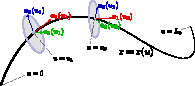
\includegraphics[width=0.8\textwidth]{figs_part2/cosserat_kinematics/cosserat_cross_section.pdf}
        \caption{Illustration of the kinematics degrees of freedom of the Cosserat rod. The black line is the \textit{center-line} $\mathbf{r}=\mathbf{r}(u)$ where $u \in [0,L_0]$ is the \textit{material coordinate} along the length of the rod, where $L_0$ is a positive real number. When specifying constitutive dynamics, $L_0$ often becomes the \textit{rest-length} of the rod. Two cross-sections at $u=u_1$ and $u=u_2$ are shown with the material frame attached $E = (\mathbf{e}_1\ \mathbf{e}_2\ \mathbf{e}_3)$, which are the red, green and blue arrows respectively, of which the latter two are the \textit{directors} of the rod. Note that having two directors, as opposed to a single director normal to the cross-section, allows for a twisting degree of freedom as can be seen in Fig.~\ref{fig:twisting cosserat rod}.}
        \label{fig:Cosserat kinematic degrees of freedom}
\end{figure}

\begin{figure*} 
    \centering
     
    \begin{subfigure}[b]{0.49\textwidth}  
        \centering 
        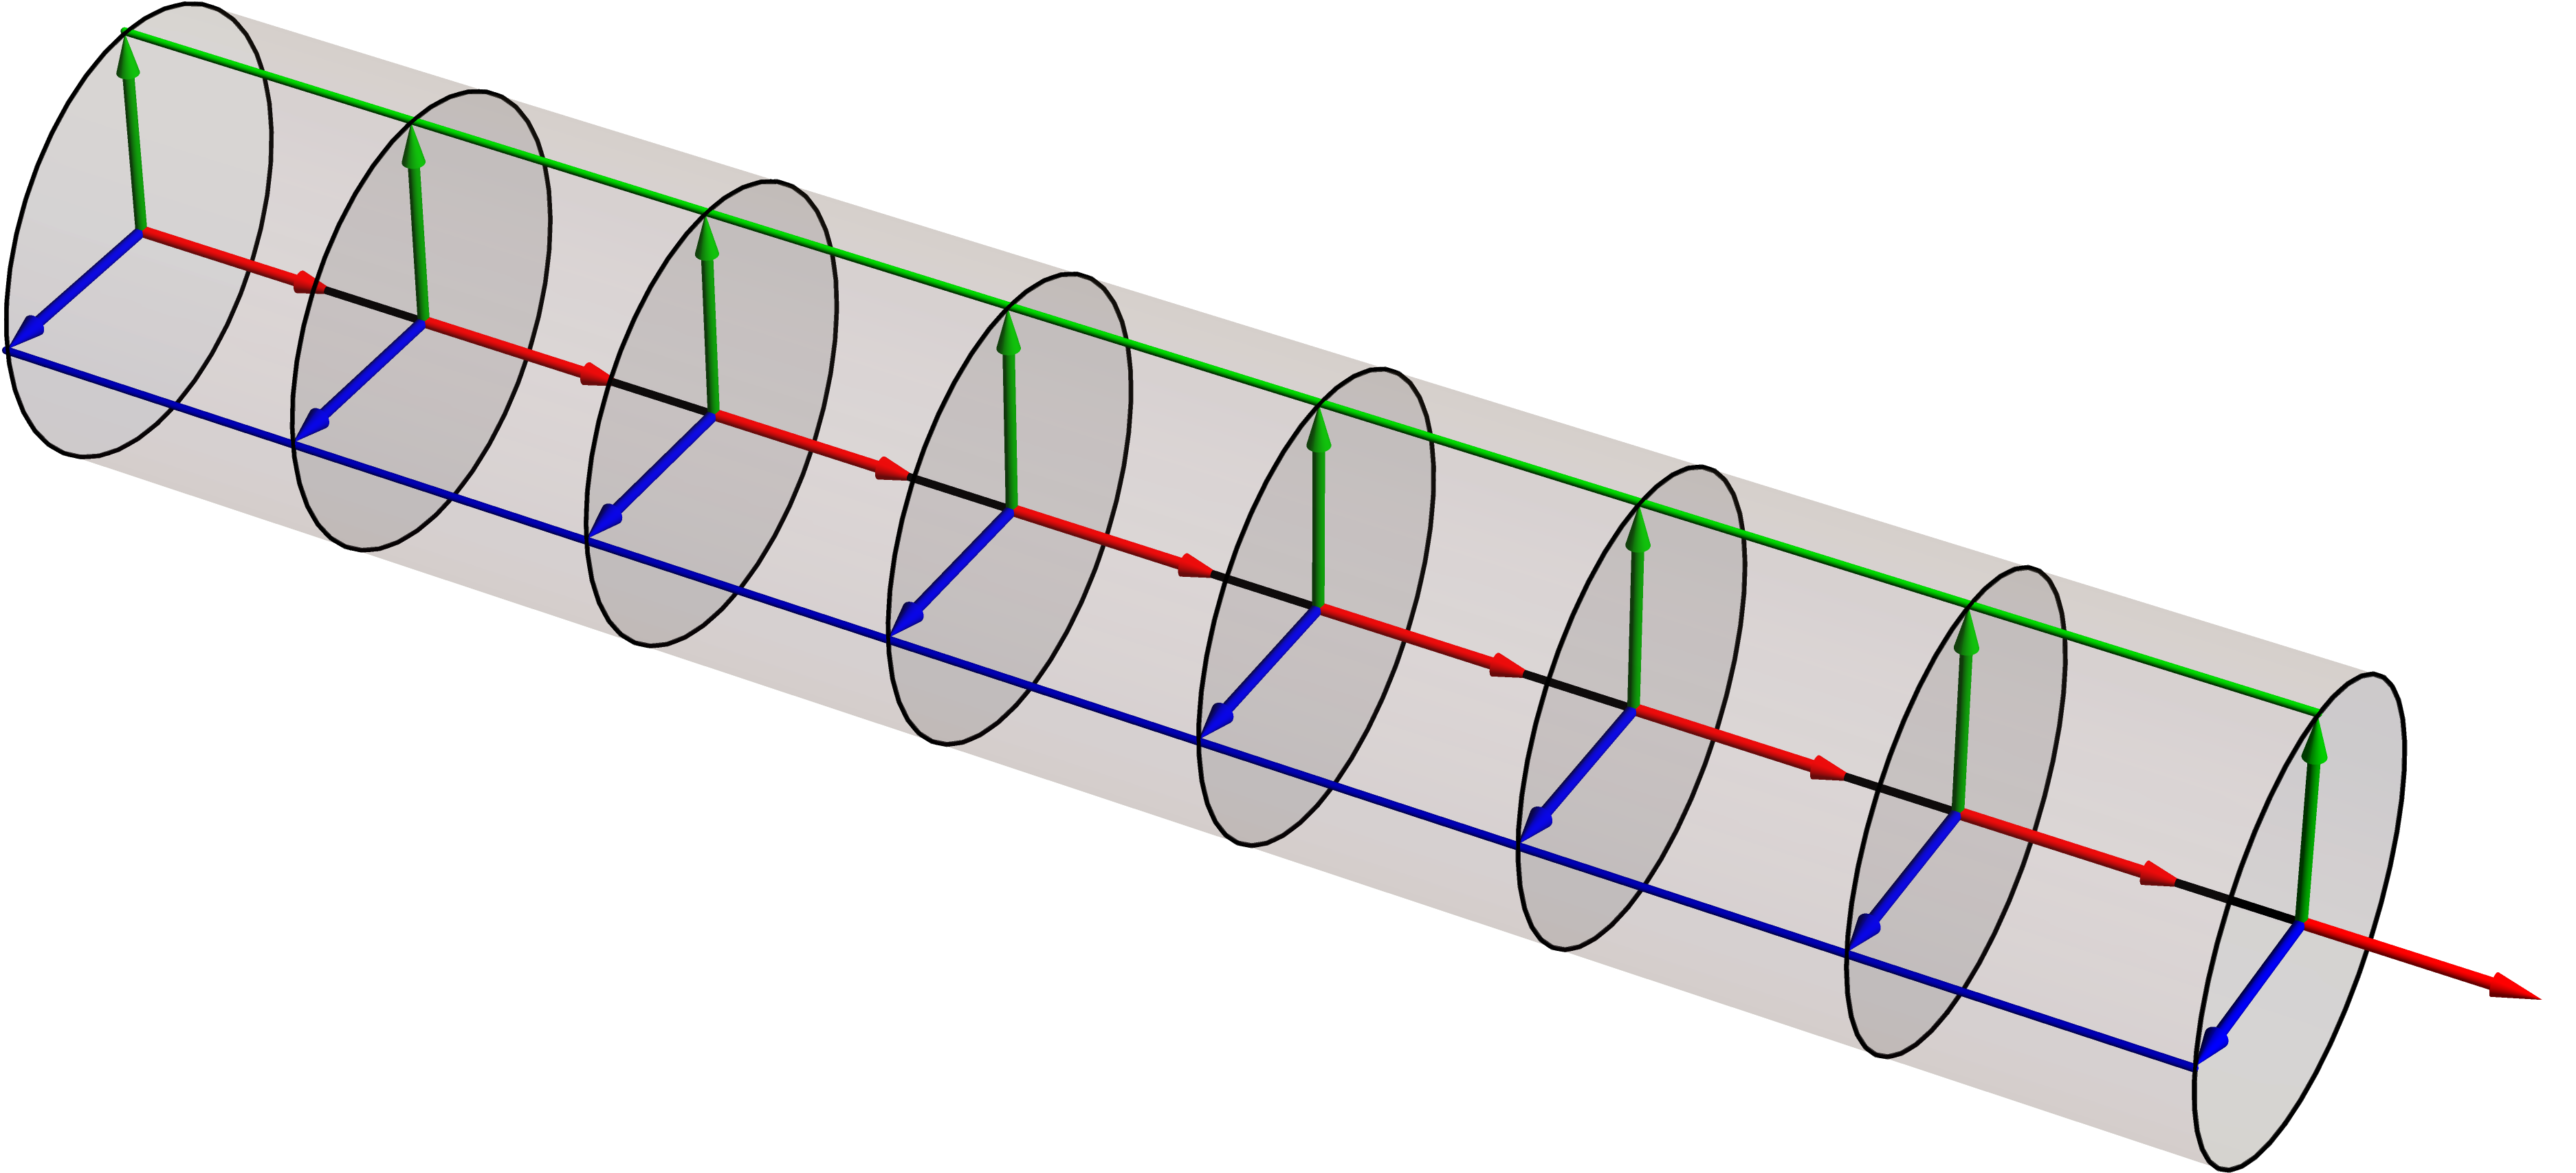
\includegraphics[width=\textwidth]{figs_part2/cosserat_kinematics/straight.png}
        \caption[Straight Cosserat rod]%
        {{\small Straight Cosserat rod}}    
        \label{fig:straight cosserat rod}
    \end{subfigure}
    \hfill
    \begin{subfigure}[b]{0.49\textwidth}
        \centering
        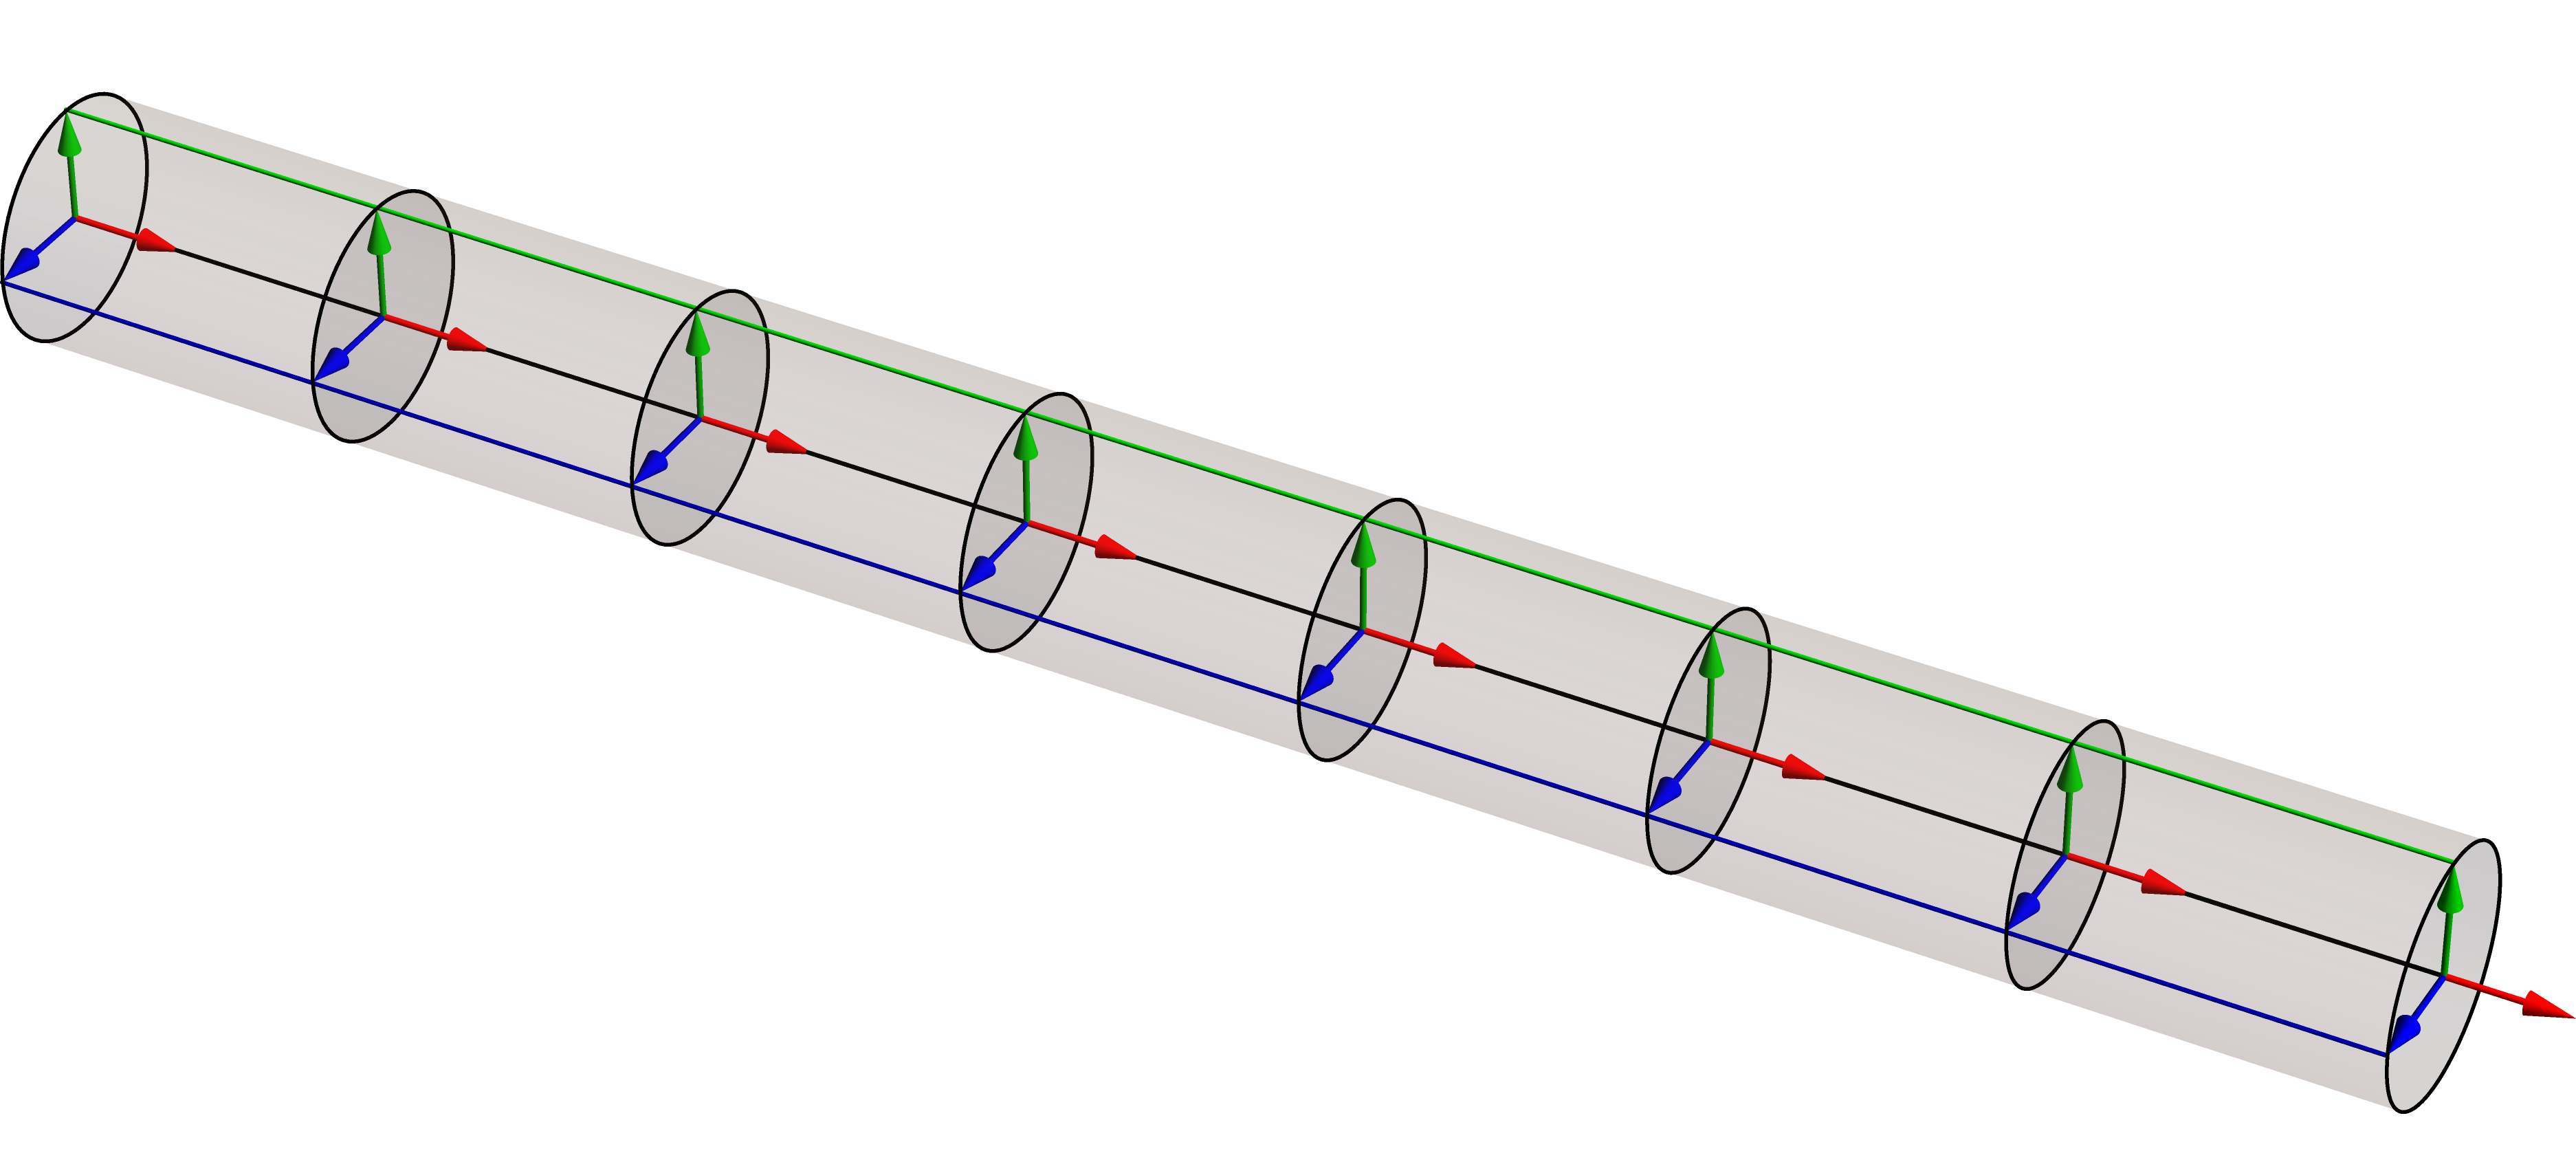
\includegraphics[width=\textwidth]{figs_part2/cosserat_kinematics/extend.png}
        \caption[Extending Cosserat rod]%
        {{\small Extending Cosserat rod}}    
        \label{fig:extending cosserat rod}
    \end{subfigure}    
    
    \vskip\baselineskip    
    \begin{subfigure}[b]{0.49\textwidth}
        \centering
        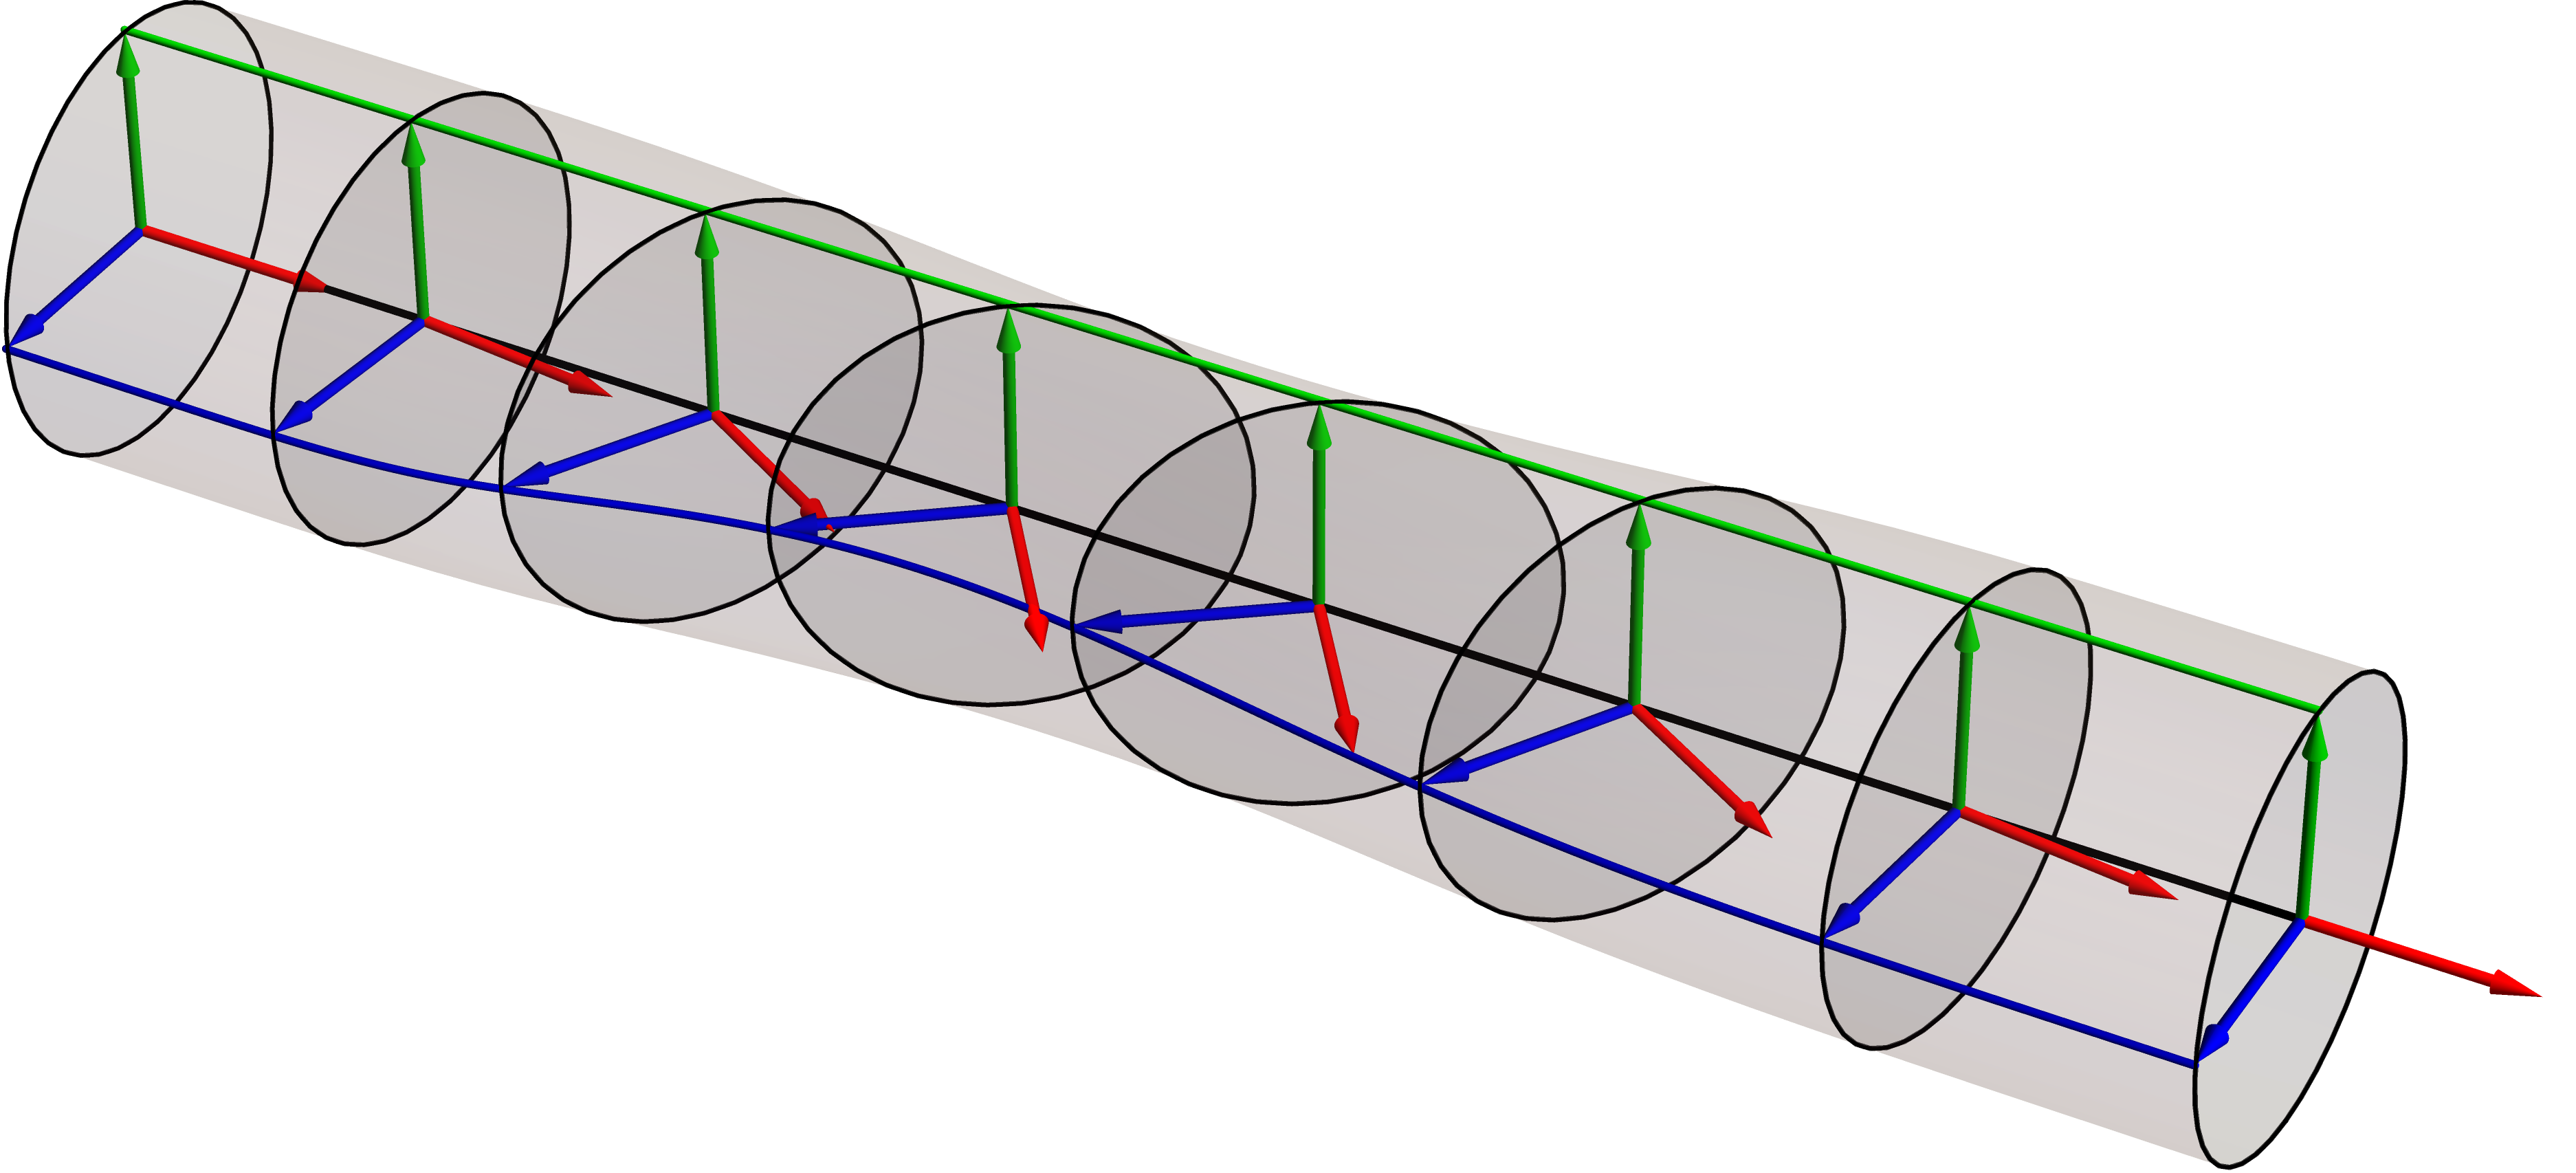
\includegraphics[width=\textwidth]{figs_part2/cosserat_kinematics/shear.png}
        \caption[Shearing Cosserat rod]%
        {{\small Shearing Cosserat rod}}    
        \label{fig:shearing cosserat rod}
    \end{subfigure}
    \hfill
    \begin{subfigure}[b]{0.49\textwidth}  
        \centering 
        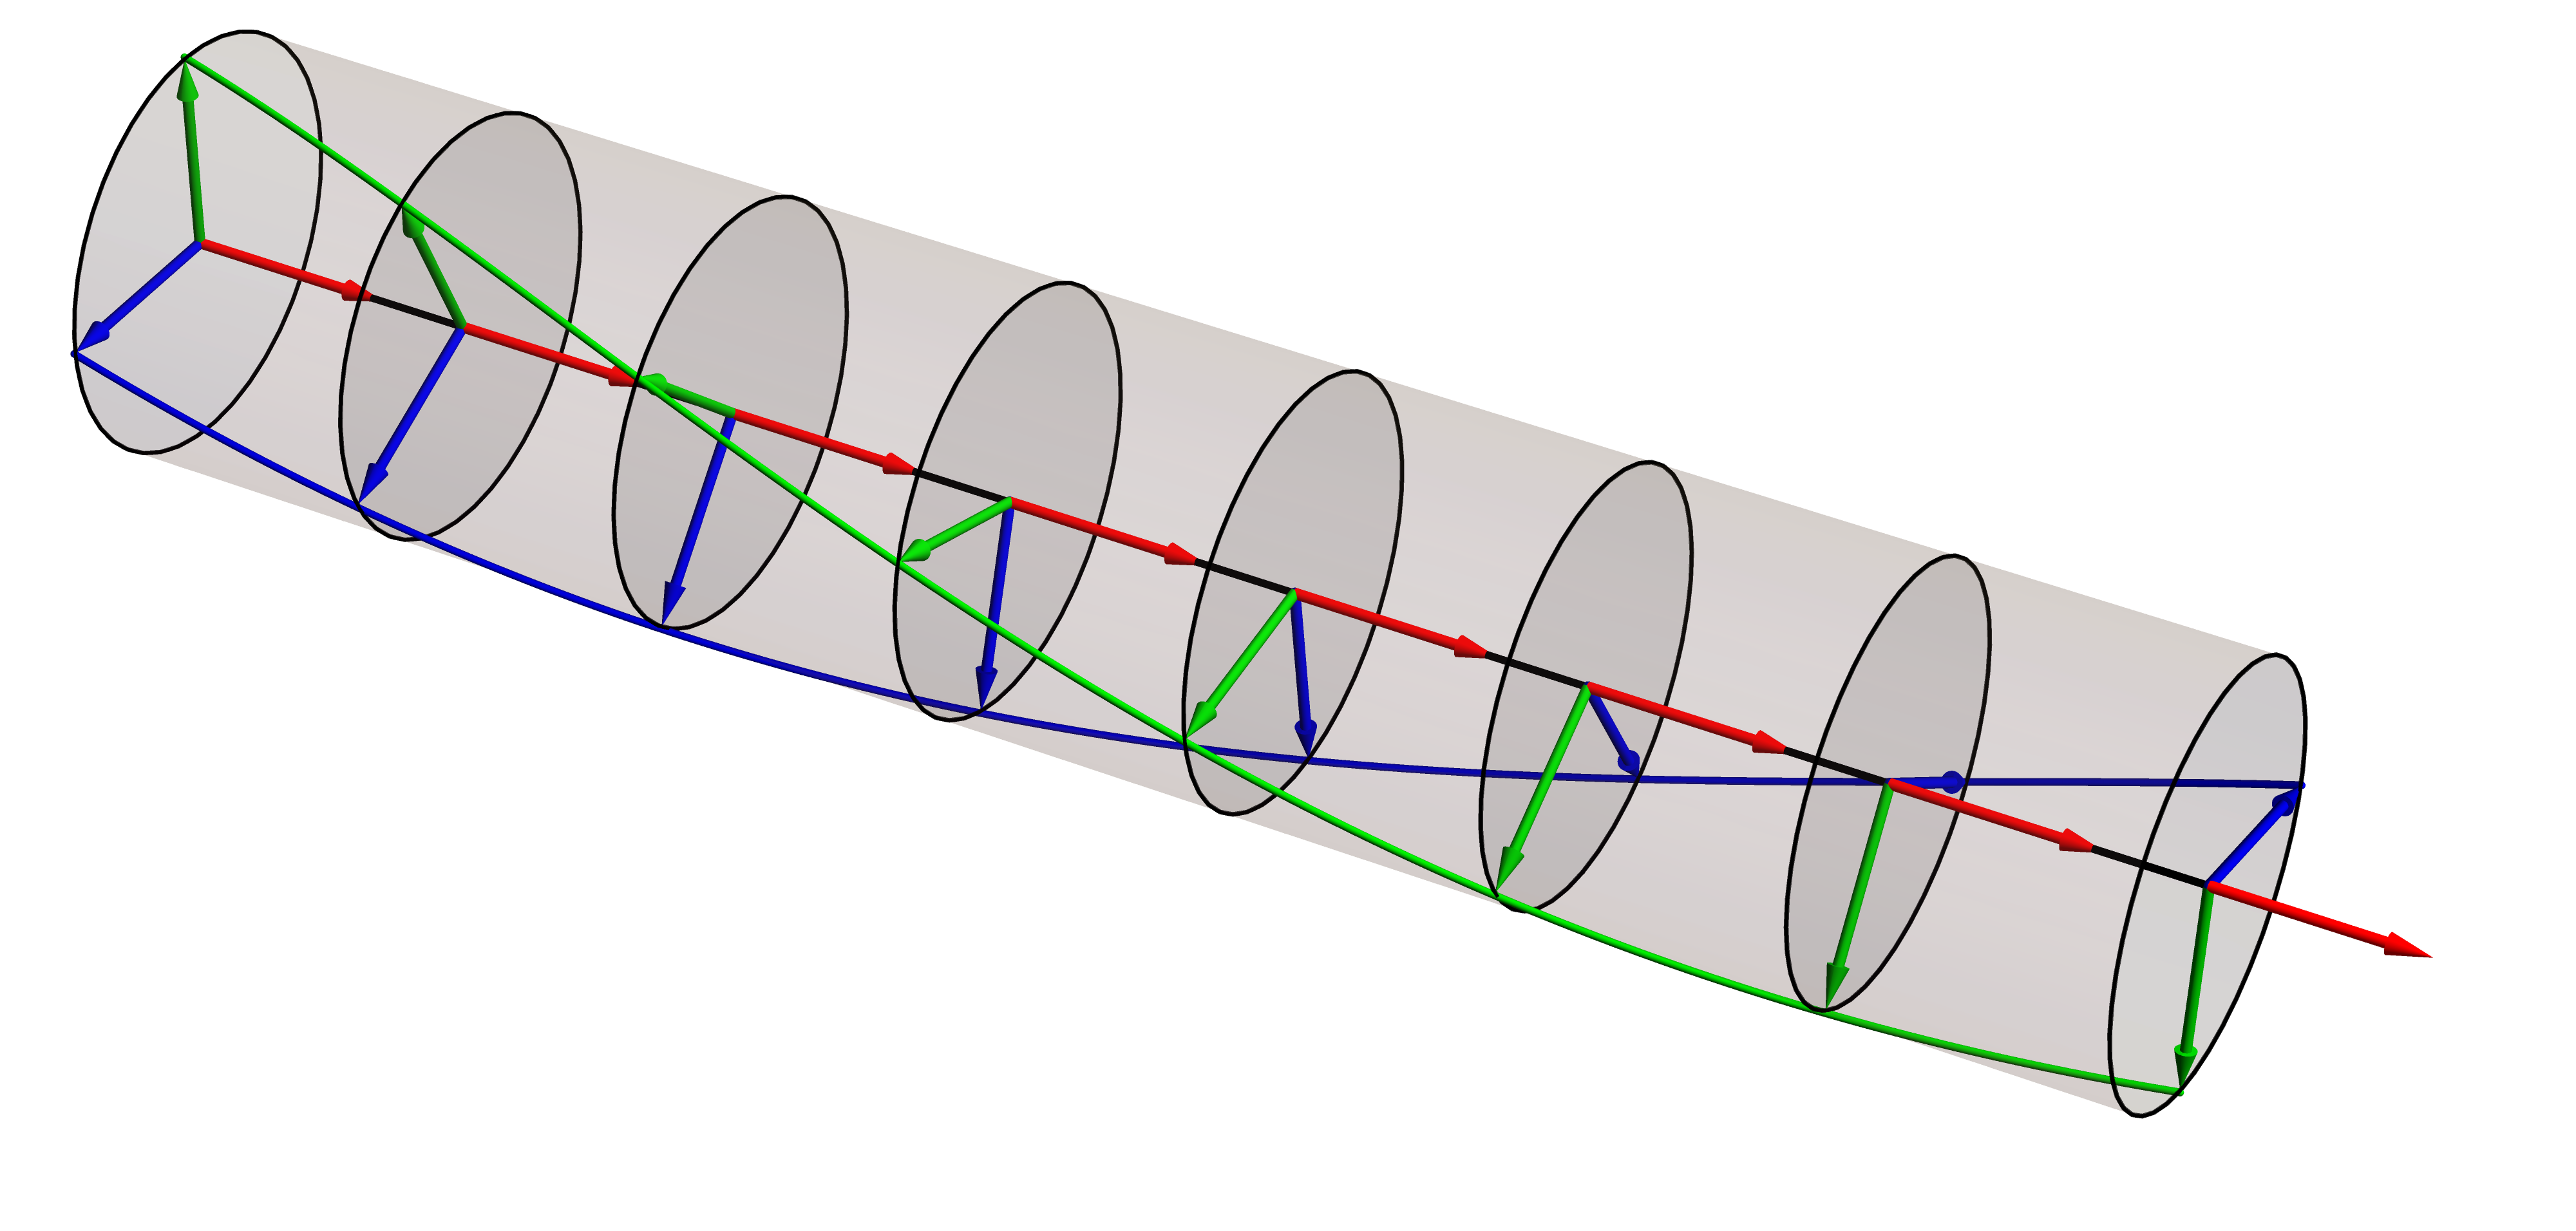
\includegraphics[width=\textwidth]{figs_part2/cosserat_kinematics/twist.png}
        \caption[Twisting Cosserat rod]%
        {{\small Twisting Cosserat rod}}    
        \label{fig:twisting cosserat rod}
    \end{subfigure}

    \vskip\baselineskip
    \begin{subfigure}[b]{0.49\textwidth}   
        \centering 
        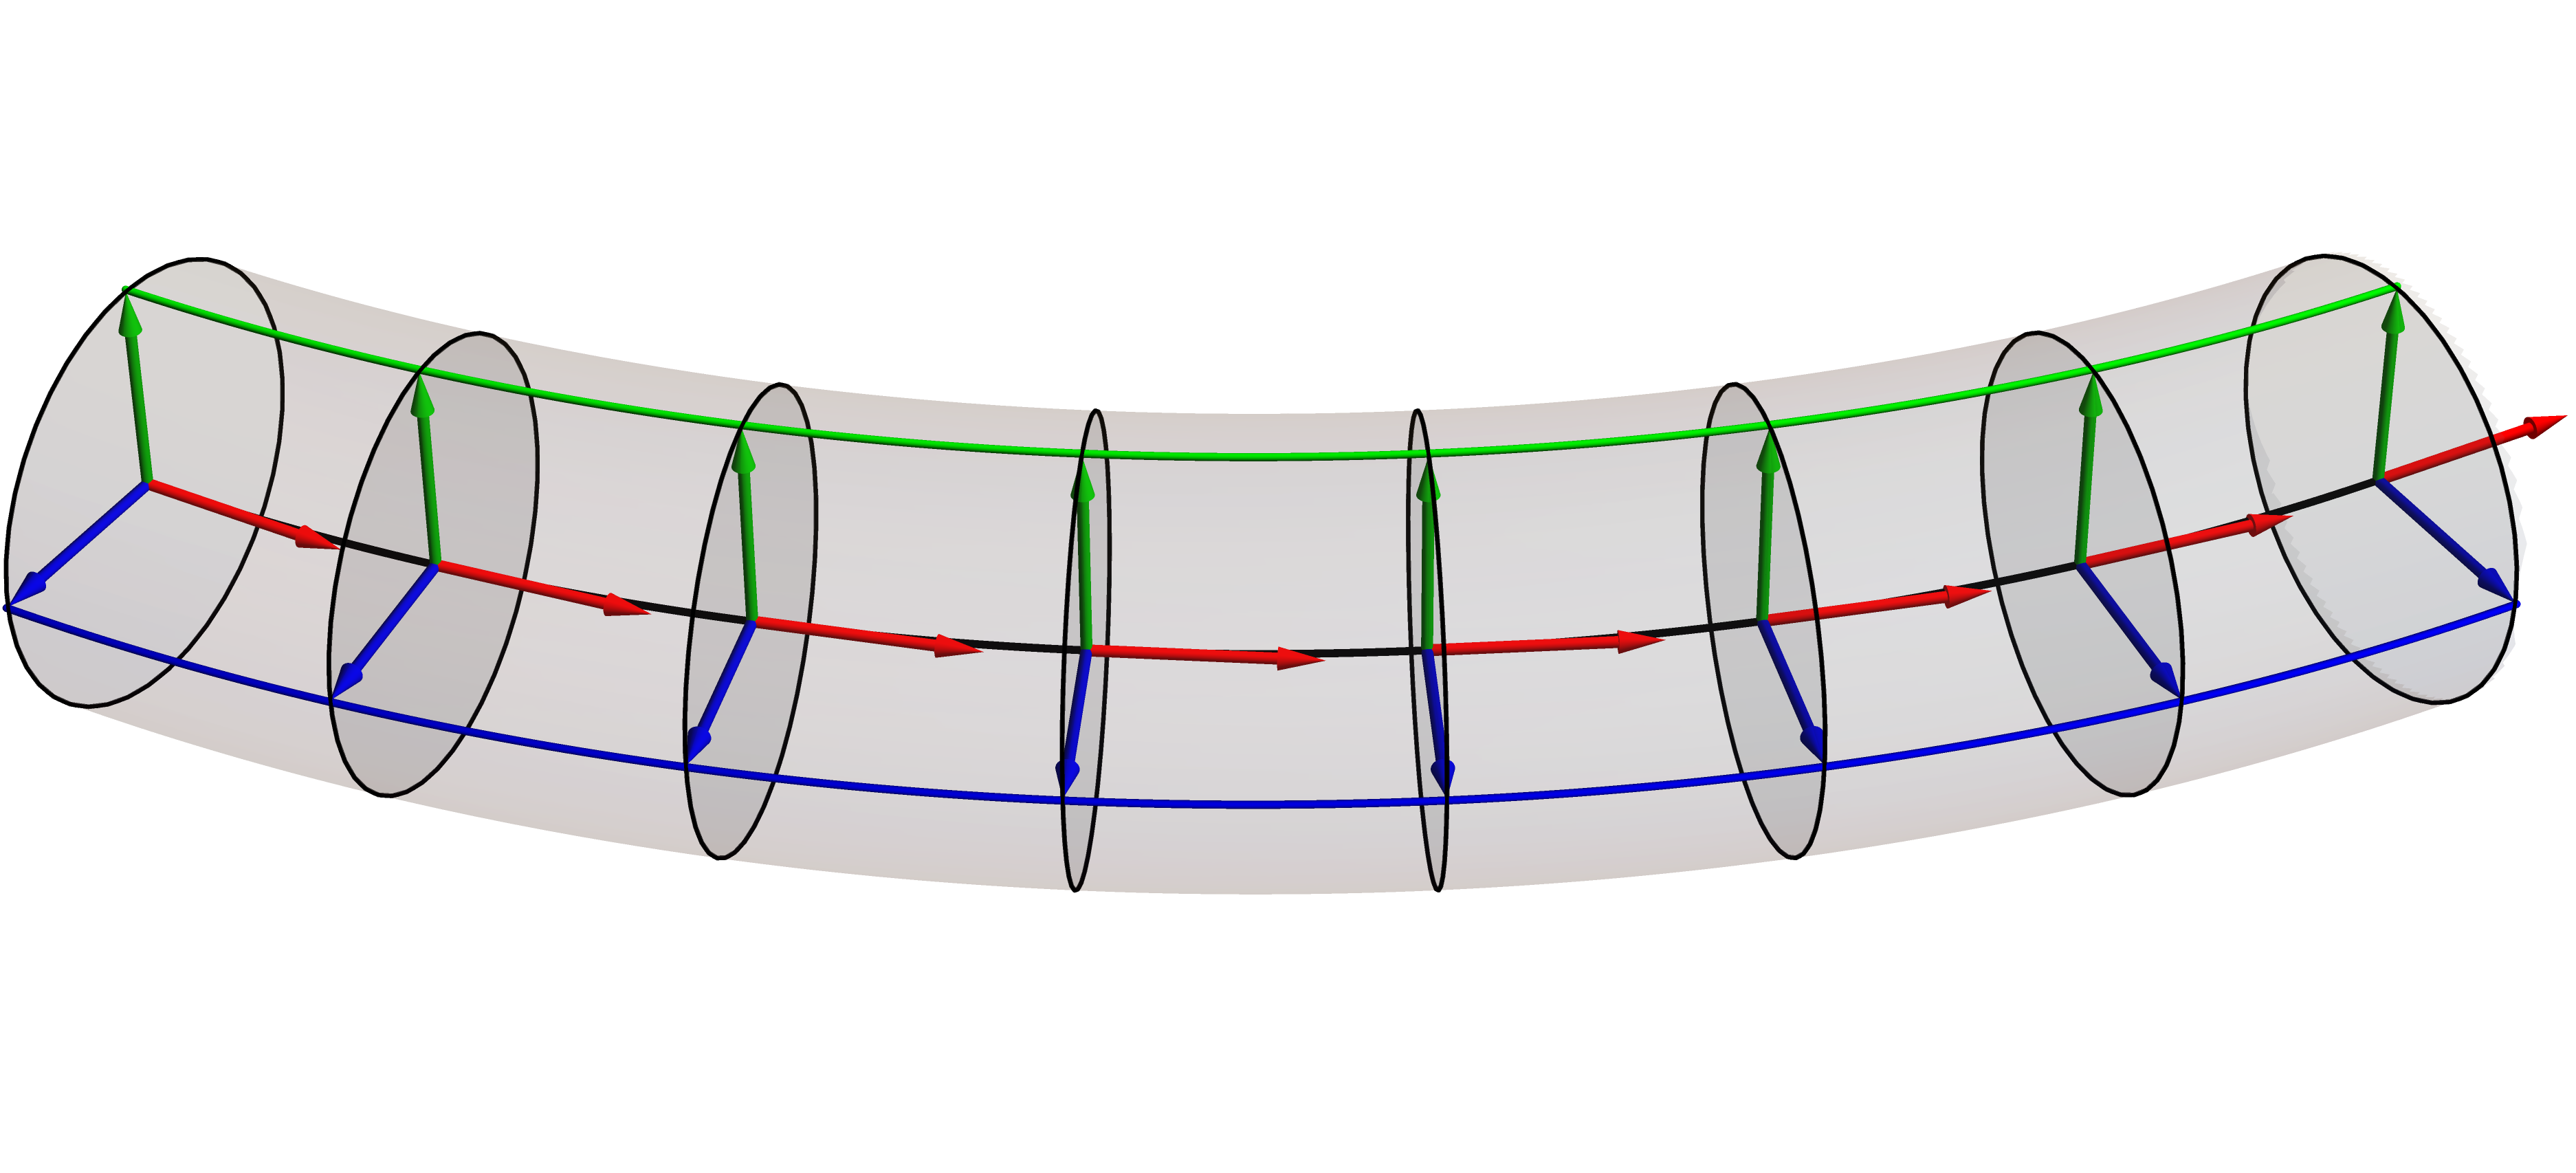
\includegraphics[width=\textwidth]{figs_part2/cosserat_kinematics/bend.png}
        \caption[Bending Cosserat rod]%
        {{\small Bending Cosserat rod}}    
        \label{fig:bending cosserat rod}
    \end{subfigure}
    \hfill
    \begin{subfigure}[b]{0.49\textwidth}   
        \centering 
        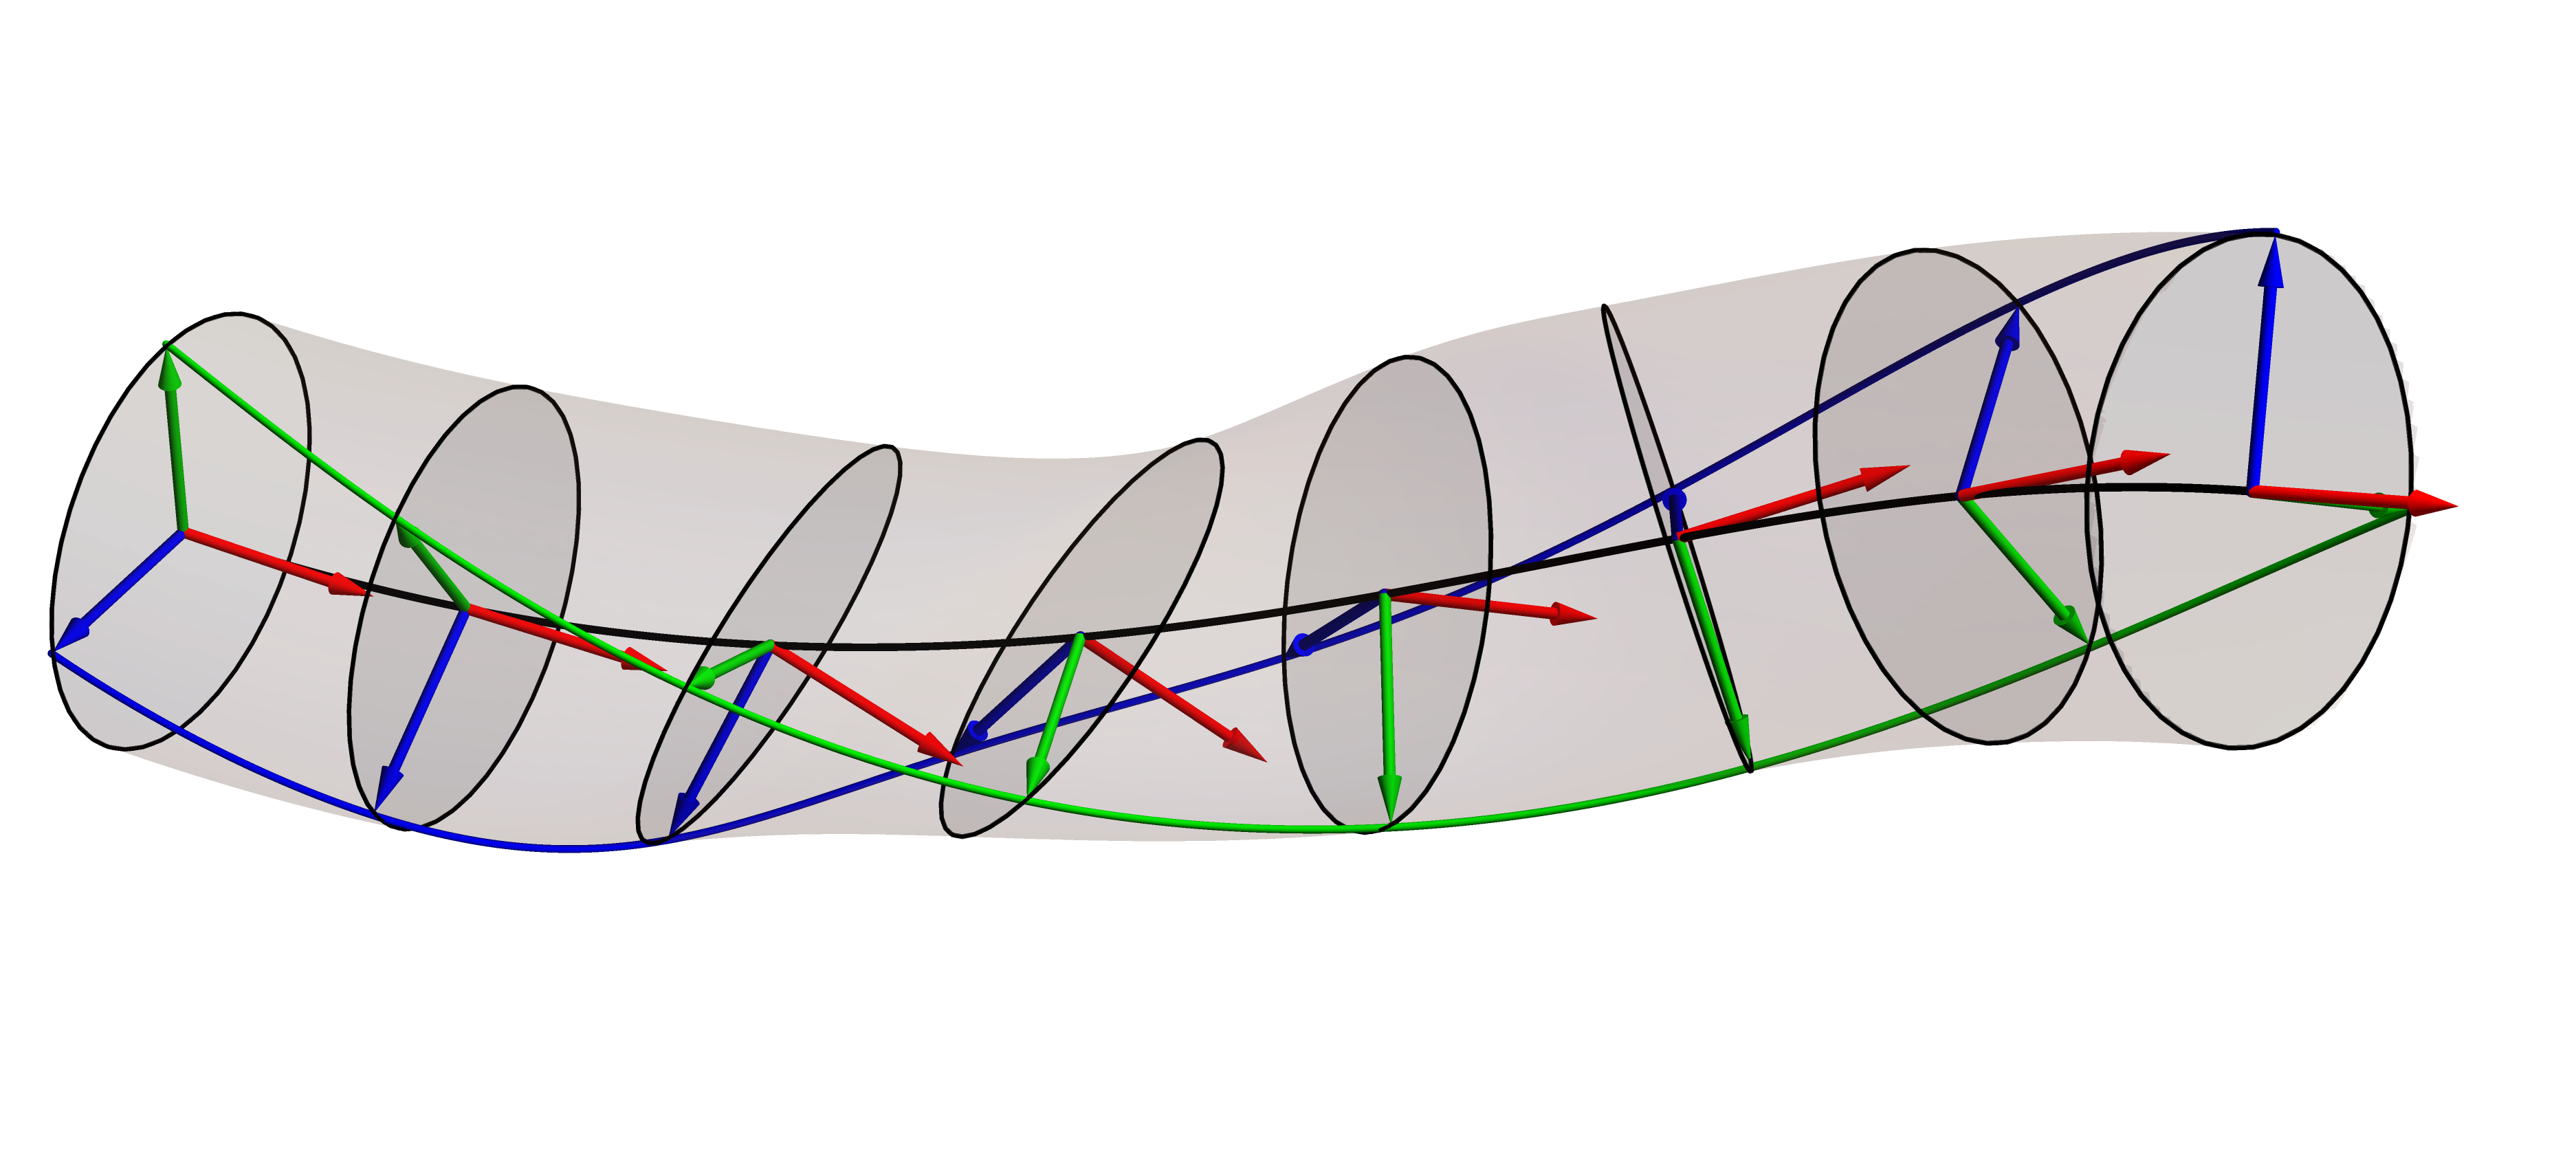
\includegraphics[width=\textwidth]{figs_part2/cosserat_kinematics/bend_shear_twist.png}
        \caption[Bending, shearing and twisting Cosserat rod]%
        {{\small Bending, shearing and twisting Cosserat rod}}    
        \label{fig:bending, shearing and twisting cosserat rod}
    \end{subfigure}
    \caption[ The average and standard deviation of critical parameters ]
    {\small Examples of deformations of the Cosserat rod. The transparent gray tubes is the bulk of the Cosserat rod, with the center-line (black line) running through its radial center. The material frame and cross-section are shown at intermittent points along the center-line, along with the surface fibres traced out by the directors $\mathbf{e}_2$ and $\mathbf{e}_3$, green and blue respectively. The tubular radii of the rods depicted were exaggerated in size for illustrative purposes. (a) A straight Cosserat rod suffering no deformation. (b-f) Examples of extension, shearing, twisting and bending deformations.} 
    \label{fig:Examples of Cosserat deformations}
\end{figure*}

A Cosserat rod can be defined as a curve in Euclidean space $\mathbf{r}(u) \in \mathbb{R}^3,\ u \in [0, L_0]$, known as the \textit{center-line} and where $L_0$ is (in a dynamical setting) the \textit{rest-length} of the rod, and an orthogonal triad $E(u) = \begin{pmatrix} \mathbf{e}_1(u) & \mathbf{e}_2(u) & \mathbf{e}_3(u) \end{pmatrix} \in \mathbb{R}^3$. The \textit{material frame} $E(u)$ represents the, in general ellipsoidal, cross-section of the rod at each \textit{material point} $u$ along the center-line. The vectors $\mathbf{e}_2(u)$ and $\mathbf{e}_3(u)$ are the aforementioned directors of the Cosserat rod, which can vary in length and represent the semi-minor and semi-major axes of the cross-section at $u$. The vector $\mathbf{e}_1(u)$ is normal to the cross-section at $u$ and is defined as $\mathbf{e}_1(u) = (\mathbf{e}_2(u) \times \mathbf{e}_3(u)) / |\mathbf{e}_2(u) \times \mathbf{e}_3(u)|$, where $\times$ is the 3-dimensional cross-product and $|\cdot|$ is the standard norm in Euclidean space.

The deformations and rotations of the center-line and material frame comprise the full kinematic degrees of freedom of the Cosserat rod. Often in applications the cross-section is approximated to be of constant shape along the rod, in which case the we restrict the directors to be inextensible and orthogonal, and thus $E(u)$ is then an orthonormal triad. See Fig.~\ref{fig:Cosserat kinematic degrees of freedom} for an illustration of a Cosserat rod with circular cross-section. In the literature this class of Cosserat rod is known as a \textit{special Cosserat rod} \citep{antmanSpecialCosseratTheory1995, rubinCosseratRods2000, altenbachCosseratMedia2013}. Henceforth, unless stated otherwise, by Cosserat rod we mean a special Cosserat rod.

The kinematic degrees of freedom of the rod are thus: smooth translations of the curve $\mathbf{r}$ and smooth rotations the material frame-field $E$. In other words, the center-line can bend, and the cross-section can shear and twist around the center-line and extend tangentially across its length, as is illustrated in Fig.~\ref{fig:Cosserat kinematic degrees of freedom}. The extension of the rod can be captured by the scalar $h(u) = \left| \frac{\partial \mathbf{r}}{\partial u} \right| $, which can be seen as the square root of the metric on the center-line induced by the Euclidean metric on $\mathbb{R}^3$. $h$ relates the material coordinate $u$ to the arc-length coordinate $s$ as
\begin{equation}
ds = h(u) du
\end{equation}
such that $ \left| \frac{\partial \mathbf{r}}{\partial s} \right| = 1$ for all $s \in [0, L]$ where
\begin{equation}
L[h(u)] = \int_0^{L_0} h(u) du
\end{equation}
is the total arc-length of the center-line. Thus any point $u$ for which $h(u)=1$ is not suffering an extension. Shear and twist deformations can be distinguished by noting that the former denotes the orientation $\mathbf{e}_1$ of the cross-section deviating from being parallel to the center-line, whilst the latter denotes rotations of the material frame around $\mathbf{e}_1(u)$. Henceforth we will also distinguish the length elements $ds$ and $du$ as the \textit{length element} and \textit{material length element} respectively.

We now add time to the picture, and consider the motion of the Cosserat rod as the result of arbitrary translational and angular velocity fields. Let the center-line $\mathbf{r}(t,u)$ and the material frame $\mathbf{e}_i(t,u)$ be functions of time, then the temporal evolution of the rod is
\begin{subequations} \label{eq:Cosserat rod kinematic equations}
  \begin{align}
\dot{\mathbf{r}} & = \mathbf{V} \label{eq:Cosserat rod r kinematic eom} \\
\dot{\mathbf{e}}_i & = \boldsymbol{\Omega} \times \mathbf{e}_i \label{eq:Cosserat rod e_i kinematic eom}
  \end{align}
\end{subequations}
from initial boundary conditions at $t=0$, and where $\mathbf{V} = \mathbf{V}(t,u)$ and $\boldsymbol{\Omega} = \boldsymbol{\Omega}(t,u)$ are arbitrary translation and angular velocities.

Dynamical equations of motion for the Cosserat rod are found by imposing balance laws on the momentum and moments of the polar continua. For undirected media, the conservation of mass and linear momentum balance are used to determine the dynamics, given constitutive and body forces. For directed media, in addition to the above, further conservation laws must be imposed to establish the director dynamics.

For a Cosserat rod with mass density $\rho_0^V$ and cross-sectional area $A$ in its reference configuration, the linear momentum of the rod is $\mathbf{P} = \rho^V_0 A \dot{\mathbf{V}}$, as is the case in classical continuum mechanics. We also introduce the director angular momentum $\mathbf{L} = I \boldsymbol{\Omega}$, where $I \in \mathbb{R}^{3 \times 3}$ is a moment of inertia matrix for the cross-section. As will be shown in Sec.~\ref{ch:Cosserat rods}, imposing the conservation of the linear momentum of the rod and the director angular momentum leads, as was first derived in \citep{cosseratTheoryDeformableBodies1909}, to
\begin{subequations} \label{eq:Cosserat rod dynamical equations of motion}
  \begin{align}
\dot{\mathbf{P}} & = \mathbf{F}' + \mathbf{f} \label{eq:Cosserat rod linear momentum balance} \\
\dot{\mathbf{L}} & = \mathbf{M}' + \mathbf{r}' \times \mathbf{F} + \mathbf{m}, \label{eq:Cosserat rod angular momentum balance} \\
\mathbf{F} & = 0,\ \text{at } u=0 \text{ and } u=L_0 \label{eq:Cosserat rod F bc}  \\
\mathbf{M} & = 0,\ \text{at } u=0 \text{ and } u=L_0 \label{eq:Cosserat rod M bc}
  \end{align}
\end{subequations}
where $\mathbf{F}$ are the constitutive forces acting on the rod, $\mathbf{f}$ the body forces per unit material length, $\mathbf{M}$ the constitutive director moments and $\mathbf{m}$ the body moment per unit material length. Eq.~\ref{eq:Cosserat rod linear momentum balance} is in a form familiar to classical continuum mechanics, which can be seen by comparing it to Eq.~\ref{eq:Cauchy momentum equation}, whilst Eq.~\ref{eq:Cosserat rod angular momentum balance} is particular to the setting of directed media. Equation \ref{eq:Cosserat rod dynamical equations of motion} and Eq.~\ref{eq:Cosserat rod kinematic equations} together form a closed set of first-order equations in time and space for the kinodynamics of a Cosserat rod.

We note here that up until this point we have considered an open Cosserat rod where $\mathbf{r}(0,t) \neq \mathbf{r}(L_0,t)$. The dynamics of a closed Cosserat rod, for which the center-line and frame are periodic functions of $u$, are identical with the exception of the omission of the boundary conditions Eq.~\ref{eq:Cosserat rod F bc} and Eq.~\ref{eq:Cosserat rod M bc}.

Equation \ref{eq:Cosserat rod dynamical equations of motion} can be derived directly from the balance laws of classical continuum mechanics, as shown in \citep{parkerDerivationNonlinearRod1984, rubinCosseratRods2000}, under the kinematic assumption that the cross-sections traced out by the directors correspond to the bulk of a three-dimensional tube of undirected point-continua. For illustrative purposes this kinematic assumption deserves further elaboration. In precise mathematical language, let $M \subset \mathbb{E}$ and let $\mathbf{x} : D \to M$ be the \textit{material coordinate} function from the domain
\begin{equation}
D = \{ (X_1, X_2, X_3)\ :\ X_1^2 + X_2^2 = R^2\ \text{and}\ X_3 \in [0,L_0]  \}
\end{equation}
where $R$ is a given fixed tubular radius of the Cosserat rod. Given a Cosserat rod configuration $(\mathbf{r},\ E)$, we define $M$ via the material coordinate function as
\begin{equation}
\mathbf{x}(\mathbf{X}) = \mathbf{r}(X_3) + X_j \mathbf{e}_j,\ j=2,3
\end{equation}
such that $M$ is the image of $\mathbf{x}$. Here the material coordinate $X_3$ corresponds to the coordinate $u$. We see how the Cosserat rod can be viewed as the result of a coarse-graining procedure from the full three-dimensional continuum setting, replacing the cross section at each $u$ with two directors, thus reducing the spatial coordinates of the system from three to one.

We now conclude this section by making some remarks, prefacing the discussions in subsequent chapters, on the geometric properties of the Cosserat rod. The kinematic equations of motion Eq.~\ref{eq:Cosserat rod r kinematic eom} and Eq.~\ref{eq:Cosserat rod e_i kinematic eom} shows explicitly that the rod moves according to infinitesimal translations $\mathbf{V}dt$ and rotations $\boldsymbol{\Omega} \times \mathbf{e}_i$ respectively. This entails that we can identify the kinematic structure of the Cosserat rod with the \textit{Lie group} of Euclidean transformations of translations and rotations $SE(3)$ \citep{simoGeometricallyexactRodModel1991, simoThreedimensionalFinitestrainRod1986}. In particular the rod itself can be parametrised in terms of sub-manifolds of $SE(3)$ and, as will be the main subject of Sec.~\ref{ch:Cosserat rods}, from which geometricised kinodynamical equations of motion can be derived programmatically. In the following section some mathematical foundations will be introduced, necessary for the subsequent chapters of this part of the thesis.

{\color{red} I think this should reference some more beneficial properties of using Lie group, like the lack of coordinitisation and some rerefernec to parameterising using the Lie algebra / differential invariants. But I can add that later when I've written the subsequent mathematical subsections. }

% Note that these equations accurately remain invariant under rigid body transformation (just make sure to look up the significance of this again).

{\color{red} Should also introduce Cosserat sheet, althouhg can do that later after you've derived the equations of motion etc.}

% In the purely mechanical three-dimensional theory the balance of angular momentum places restrictions on the constitutive equations which require the Cauchy stress tensor to be symmetric. Also, the conservation of mass and the balance of linear momentum are used to determine the mass density and the position of each material point in the continuum. For the Cosserat theories that will be developed in the next chapters, alternative equations representing the conservation of mass and the balances of linear and angular momentum will be used in a similar manner to determine the mass density and the position of each material point. However, the Cosserat theories will introduce additional kinematical quantities called director vectors at each material point which also need to be determined by additional balance laws. In order to motivate the forms for these balance laws, it is convenient to consider an averaged form of the balance of linear momentum

% The global forms of the balance laws of the Cosserat theory of shells are similar to those of the three-dimensional theory in the sense that they include the notions of conservation of mass and balances of linear and angular momentum. Moreover, these equations are used to determine the current values of a mass density p and the position vector x of points on the surface 5 of the shell. Also, the balance of angular momentum places restrictions on the constitutive equations of the shell theory that are similar in nature to the restrictions (3.2.32) associated with the three-dimensional theory. However, in contrast with the three-dimensional theory, the Cosserat theory of shells introduces the additional kinematic quantity d3 at each point of the surface 5 of the shell which also must be determined by a balance law. Consequently, the Cosserat theory of shells requires an additional balance law called the balance of director momentum.

% In this section it will be shown that the balance laws of the Cosserat theory can be developed by using the kinematic assumption (4.2.7) and the balance laws of the threedimensional theory.



%- Define the polar continua precisely that we are interested in: Cosserat rod with orthonormal directors. Figures:
%  - One figure (perhaps just in Inkscape, like the one you've made earlier) that just shows the cross section.
%  - Show the twisting, bending and shearing degrees of freedom. These should be 3D. In Mathematica you should write code that can take in cosserat data and spit out a 3D model figure.
%- Introduce the kinematic and dynamics equations of motion, in terms of $\mathbf{r}$ and $\mathbf{e}_i$. 
%- Note that these equations accurately remain invariant under rigid body transformation (just make sure to look up %the significance of this again).
%- Note that the equations move according to Euclidean transformation, motivates the subsequent sections.

\section{Mathematical preliminaries}

As will be further discussed in Ch.~\ref{ch:Cosserat rods}, directed media can be seen as either sub-manifolds of \textit{homogeneous spaces} or sub-manifolds of \textit{Lie groups}. Through this lens, a fully geometricised and non-coordinate form of the equations of motion of such systems can be derived. This section serves primarily to establish establish the mathematical foundation and rigour of the programme, and therefore has a level of mathematical abstraction higher than that of the subsequent chapters. The reader not interested in these details may proceed to Ch.~\ref{ch:Cosserat rods}, and return to this section intermittently to fill gaps in notation and conceptual knowledge.

For a fuller treatment of the concepts introduced in this section the reader can consult the following references for further exposition \citep{clellandFrenetCartanMethod2017, kleinDevelopmentMathematics19th1979, marsdenIntroductionMechanicsSymmetry2013, marleHenriPoincareNote2013a}.

\subsection{Differential geometry}

Pullbacks and pushforwards

Define the Lie bracket in component form

\begin{equation} \label{eq:lie bracket in component form}
[X, Y] = (X^j \partial_j Y^i - Y^j \partial_j X^i) \partial_i
\end{equation}

\subsection{Exterior calculus}

In calculus, the differential of a scalar function $f : \mathbb{R}^3 \to \mathbb{R}$ is often written as
\begin{equation}
df = \frac{\partial f}{\partial x} d x + \frac{\partial f}{\partial y} d y + \frac{\partial f}{\partial z} d z.
\end{equation}
This can be generalised for differentiable manifolds. Let $M$ be a smooth $d$-dimensional manifold, $p \in M$ a point on the manifold, $X \in \Gamma(TM)$ a vector field on $M$ and $f \in C^\infty(M)$ be a smooth function on $M$. We define the map $df : TM \to \mathbb{R}$ as
\begin{equation} \label{eq:df action}
(df(X))(p) = X_p(f).
\end{equation}
Here $df$ is an example of a \textit{scalar-valued $1$-form}. Analogously, scalar functions $f \in C^\infty(M)$ are known as \textit{scalar-valued $0$-forms}. Scalar-valued $p$-form are linear maps $\prod_{i=1}^p TM \to \mathbb{R}$, where $\prod$ signifies the repeated Cartesian product. The operator $d$ is the \textit{exterior derivative}, which in general maps $p$-forms to $(p+1)$-forms. Any $(p+1)$-form that can be written as the exterior derivative of a $p$-form is referred to as \textit{exact}. Conversely, any $p$-form $\phi$ that satisfies $d \phi = 0$ is \textit{closed}. Locally, closed $p$-forms are always exact, which is known as the \textit{Poincaré lemma}. 
 
Let $x^i : U \to \mathbb{R},\ i=1,\dots,d$ be coordinate functions for some neighbourhood $U \subset M$. Then $df$ can then be locally expressed in in $U$ as
\begin{equation} \label{eq:df expansion}
df = \frac{\partial f}{\partial x_i} d x^i
\end{equation}
such that $df(X) = \frac{\partial f}{\partial x^i} dx^i(X) = \frac{\partial f}{\partial x^i} X^i$, where $X \in \Gamma(TM)$. Not all $1$-forms are closed, and can thus not be written in the form of Eq.~\ref{eq:df expansion}, but they can always be expanded in a coordinate basis as $\phi = a_i dx^i$, where $a_i \in C^\infty(M),\ i=1,\dots,d$ are the coefficients of $\phi$ in this basis.

The \textit{symmetric product} of a $p$-form $x$ and $q$-form $y$ is written as $x \otimes y$. For $p=q=1$, we have
\begin{equation}
(x \otimes y)(X, Y) = \phi(X) \psi(Y)
\end{equation} 
where $X, Y \in \Gamma(TM)$ are two vector fields. For a general $1$-form, its exterior derivative can be expressed locally as
\begin{equation} \label{eq:exterior derivative of 1-form}
d\phi = d a_i \wedge dx^i.
\end{equation}
where $\wedge$ is the \textit{wedge product}. Let $x$ and $y$ be a $p$-form
and a $q$-form respectively, then $x \wedge y$ is a $(p+q)$-form defined as
\begin{equation}
x \wedge y = x \otimes y - y \otimes x
\end{equation}
and satisfies
\begin{equation}
y\wedge x=(-1)^{pq}x\wedge y.
\end{equation}
and
\begin{equation} \label{eq:exterior derivative of wedge product}
d(x \wedge y) = dx \wedge y + (-1)^p x \wedge d y.
\end{equation}
The wedge product of a sequence of forms can be written as
\begin{equation}
\bigwedge_{i=1}^n z^i = dz^1 \wedge dz^2 \wedge \dots \wedge dz^n
\end{equation}
where each $z^i$ is a $p^i$-form. Due to the anti-symmetry of the wedge products of $1$-forms, we have
that $df \wedge df = 0$ for any $f \in C^\infty(M)$. If $x$ and $y$ are two $1$-forms, then the product $x \wedge y$ is a mapping $TM \times TM \to \mathbb{R}$, and can be evaluated on two vector fields $X,Y \in \Gamma(M)$ as
\begin{equation}
(x \wedge y)(X, Y) = x(X) y(Y) - x(Y) y(X).
\end{equation}

We will now derive a coordinate-free expression for the exterior derivative of a $1$-form. Let $\phi = a_i dx^i$, then
\begin{equation} \label{eq:exterior derivative of 1-form evaluated}
\begin{aligned}
d\phi(X,Y) & = da_i(X) Y^i - da_i(Y) X^i \\
 & = \frac{\partial a_i}{\partial x^k} X^k Y^i - \frac{\partial a_i}{\partial x^k} Y^k X^i \\
 & =  \left( X^k \frac{\partial}{\partial x^k} ( a_i Y^i) - a_i X^k \frac{\partial Y^i}{\partial x_k} \right) -  \left( Y^k \frac{\partial}{\partial x^k} ( a_i X^i) - a_i Y^k \frac{\partial X^i}{\partial x_k} \right) \\
 & = X^k \frac{\partial}{\partial x^k} ( a_i Y^i) - Y^k \frac{\partial}{\partial x^k} ( a_i X^i) - a_i  \left( X^k \frac{\partial Y^i}{\partial x_k} - Y^k \frac{\partial X^i}{\partial x_k} \right) \\
 & = X(\phi(Y)) - Y(\phi(X)) - \phi([X,Y])
\end{aligned}
\end{equation}
where we used Eq.~\ref{eq:lie bracket in component form}.

Intuitively, a $1$-form can be seen as measuring an infinitesimal oriented length. A $2$-form can be seen as measuring an infinitesimal oriented area. A $p$-form measures an infinitesimal oriented $p$-dimensional volume. There is therefore a natural notion of integrals of $p$-forms. In general, a $p$-form $\phi$ defined on a manifold $M$ can be integrated on a $p$-dimensional sub-manifold of $M$.

If $M$ is $d$-dimensional, then the integration of $d$-forms and $1$-forms coincides with the usual notion of integration in multi-variate calculus. Let $U \subset M$ with coordinates $x^i : U \to \mathbb{R}^d$, and let $\gamma \subset U$ be a $1$-dimensional sub-manifold of $U$, and let $\phi = h_i dx^i$ be a general $1$-form and $\psi = g \bigwedge_{i=1}^d dx^i$ a general $d$-form then
\begin{subequations}
\begin{align}
\int_\gamma \phi & = \int_\gamma h_i d x^i \\
\int_U \psi & = \int_U g \bigwedge_{i=1}^d dx^i = \int_U g\ dx^1 dx^2 \dots dx^d
\end{align}
\end{subequations}
where the right-most term in the equalities are the standard multi-variate integrals. For a $d$-dimensional manifold, a $d$-form like $\psi$ is called a \textit{volume form}. If $V \subset M$ is a $(p-1)$-dimensional sub-manifold and $\phi$ is a $p$-form, then it can be shown that
\begin{equation} \label{eq:stokes theorem}
\int_V d \phi = \int_{\partial V} \phi
\end{equation}
where $\partial V$ signifies the boundary of $V$. Eq.~\ref{eq:stokes theorem} is called \textit{Stokes' theorem}.

Consider a $1$-form expressed locally as $\phi = a_i dx^i$. Under change of coordinates, it transforms as
\begin{equation} \label{eq:dx transform}
a_i dx^i = a_i \frac{\partial x^i}{\partial \tilde{x}^i} d\tilde{x}^i.
\end{equation}
From Eq.~\ref{eq:dx transform}, it can be shown that $d$-forms transform as
\begin{equation}
f \bigwedge_{i=1}^d dx^i = \left( \text{det} \left[ \frac{\partial \mathbf{x} }{ \partial \tilde{\mathbf{x}} } \right] f \right) \bigwedge_{i=1}^d d\tilde{x}^i
\end{equation}
where $\frac{\partial \mathbf{x} }{ \partial \tilde{\mathbf{x}} }$ is the Jacobian matrix of the coordinate transformation.

\subsection{Lie groups}

\begin{definition}
A $d$-dimensional \textit{Lie group} is a set $G$ that is both a group and a differentiable manifold of dimensions $d$, where the multiplication map $G\times G \to G$
\begin{equation}
(g,h) \mapsto gh \in G
\end{equation}
and inverse $G \to G$
\begin{equation}
g \mapsto g^{-1}
\end{equation}
are smooth maps.
\end{definition}

For all Lie groups $G$ under consideration in this text the group elements in $G$ can be represented as invertible matrices. In other words, there is a map $\Pi : G \to GL(V)$, where $GL(V)$ is the Lie group of linear operators with non-zero determinant acting on some $n$-dimensional vector space $V$. Such a map is called a \textit{representation} of $G$. For all Lie groups there is a canonical \textit{fundamental representation} $g : G \to GL(\mathbb{R}^{n})$, and we will often identify the image $g(G) = \tilde{G}$ with the Lie group itself. Henceforth, unless explicitly stated to be otherwise, we will use the shorthand $g \in G$, identifying the Lie group elements in their fundamental representation with the Lie group elements themselves.

For each element $g \in G$, the \textit{left multiplication} map $L_g : G \to G$ is defined as $L_g h = gh$ where $h \in G$. Similarly, the \textit{right multiplication} map $R_g : G \to G$ is defined as $R_g h = hg$. For maps between smooth manifolds $\Psi : M \to N$, we define its \textit{derivative} at $p \in M$ as the mapping $D\Psi_p : T_p M \to T_{\Phi(p)} N$ given by the formula
\begin{equation} \label{eq:derivative of linear map}
D\Psi_p (v)(f) = v(f \circ \Psi)
\end{equation}
for $v \in T_p M$ and $f \in C^\infty(N)$. In particular, the derivative of the left multiplication at $h\in G$ is a mapping $(DL_g)_h : T_hG \to T_{gh} G$, which can be shown to be equal to
\begin{equation}
(DL_g)_h(X) = gX
\end{equation}
where $X \in T_h G$. For any Lie group $G$ there is an associated \textit{Lie algebra} $\mathfrak{g}$, which is the tangent space $T_e G$ at the identity, where $e \in G$ is the identity element. $\mathfrak{g}$ is thus a vector space of the same dimension $d$ as $G$. For any vector $W \in \mathfrak{g}$, we can define a \textit{left-invariant vector field} $\tilde{W}$ defined on each $g \in G$ as
\begin{equation} \label{eq:left-invariant vector field}
\tilde{W}_g = (DL_g)_e (W).
\end{equation}
Now let $E_i,\ i=1,\dots,d$ be a basis for $\mathfrak{g}$, then it can be shown that the corresponding left-invariant vector-fields $\tilde{E}_i$ form a global basis for the tangent bundle $TG$. This implies that the tangent bundle of Lie groups $G$ are isomorphic to the Cartesian product $TG \cong G \times \mathfrak{g}$. Furthermore, it is notable that the global basis is constructed without specifying coordinate functions on the manifold.

The \textit{exponential map} $\exp : \mathfrak{g} \to G$ relates Lie algebra elements to corresponding Lie group elements, and for matrix Lie groups this is explicitly given by the matrix exponential. Intuitively this mapping can be understood by considering the curve $\gamma(t) = \exp ( t V ) \in G$, where $W \in \mathfrak{g}$. Differentiating the curve gives us
\begin{equation}
\begin{aligned}
\frac{d}{dt} \gamma(t) & = \exp (t W) W \\
& = (D L_{ \exp (t W) } )_e (W) = \tilde{W}_g
\end{aligned}
\end{equation}
The curve $\gamma$ is thus a flow-line of the left-invariant vector field $\tilde{W}$.

The Lie algebra $\mathfrak{g}$ also has a product structure known as the \textit{Lie bracket} $[\cdot, \cdot] : \mathfrak{g} \times \mathfrak{g} \to \mathfrak{g}$ given by
\begin{equation}
[X, Y] = XY - YX
\end{equation}
for $X,Y \in \mathfrak{g}$. To see its relation to the Lie group, we introduce the \textit{adjoint action} of a Lie group on its Lie algebra  $\text{Ad} : G \times \mathfrak{g} \to \mathfrak{g}$ given by
\begin{equation}
\text{Ad}_g Y = g Y g^{-1}
\end{equation}
for each $g\in G$, $\text{Ad}_g$ is thus an automorphism of the Lie algebra. Let $g(t) = \exp(t X)$, with Taylor expansion $g(t) = I + t X + O(t^2)$. The the infinitesimal action of the automorphism $\text{Ad}_g$ can then be found by expanding it as
\begin{equation}
\text{Ad}_g Y = Y + t[X, Y] + O(t^2).
\end{equation}
This motivates the definition of the adjoint action of the Lie algebra \textit{on itself} $\text{ad} : \mathfrak{g} \times \mathfrak{g} \to \mathfrak{g}$ given by
\begin{equation}
\text{ad}_X Y = [X, Y].
\end{equation}
Let $E_a,\ a=1,\dots,d$ be a basis for Lie algebra $\mathfrak{g}$, then the Lie bracket can also be written in terms of its \textit{structure constants} $f^a_{bc} \in \mathbb{R}$
\begin{equation}
[E_a, E_b] = f_{ab}^c E_c, \quad a,b,c=1,\dots,d.
\end{equation}
The Lie algebra can be \textit{defined} as a vector space $\mathfrak{g}$ equipped with Lie bracket, where the latter is fully specified by the structure constants. If $G$ is connected, then $G$ is exactly equal to the image of $\mathfrak{g}$ under the exponential map \footnote{If $G$ is not connected, $\exp(\mathfrak{g})$ is equal to the sub-group of $G$ that is connected to the identity element $e \in G$.}. This is known as the \textit{Lie algebra-Lie group correspondence}. We thus see that the structure constants encapsulates the full geometry of the Lie group.

For a $d$-dimensional Lie group $G$, with Lie algebra $\mathfrak{g}$, a linear map $\prod_{i=1}^p TG \to \mathfrak{g}$ is a \textit{Lie algebra-valued} $p$-form. A general Lie algebra-valued $1$-form $X : TG \to \mathfrak{g}$ can be written as
\begin{equation}
X = a_i^a E_a dx^i
\end{equation}
where $E_a,\ a=1,\dots,d$ is a basis for $\mathfrak{g}$, $x^i \in C^\infty(G),\ i=1,\dots,d$ are global coordinate functions on $G$, and $a_i^a \in C^\infty(G),\ i,a=1,\dots,d$ are the coefficients of $X$ in this basis. The exterior derivative of a Lie-algebra valued form can be computed by simply applying it directly on the scalars in the expression. For example, the exterior derivative of a Lie algebra-valued $1$-form is
\begin{equation}
dX = E_a\ d(a_i^a dx^i).
\end{equation}
Similarly, let $Y = b_i^a E_a dx^i$, then the wedge product of two $1$-forms can be computed as
\begin{equation}
X \wedge Y = E_a E_b a_i^a b_j^b\ dx^i \wedge dx^j
\end{equation}
where $E_a E_b$ denotes ordinary matrix multiplication. Note that the wedge product of two Lie algebra-valued forms is not necessarily Lie algebra-valued.

Finally we note that for any Lie group representation $\Pi : G \to GL(V)$, there is a corresponding representation $\rho : \mathfrak{g} \to \mathfrak{gl}(V)$ of the Lie algebra, that are related as $\exp(\rho(W)) \in \Pi(G)$ for any $W \in \mathfrak{g}$. As with Lie groups, there is a canonical fundamental representation of the Lie algebra as linear maps $\mathfrak{gl}(\mathbb{R}^{n})$, and we identify this representation with $\mathfrak{g}$ itself.

The following are some examples of Lie groups:
\begin{itemize}
\item The general linear group $GL(V)$ is the set of linear maps with non-zero determinant acting on a vector space $V$.

\item The positive real numbers $\mathbb{R}^+$ equipped with multiplication forms an \textit{abelian} Lie group, where all elements commute with each other.

\item The orthogonal group $O(n)$ which is the space of orthogonal $n \times n$ matrices. Its Lie algebra $\mathfrak{o}(n)$ comprises the space of anti-symmetric $n \times n$ matrices.

\item The special orthogonal group $SO(n)$ is the set of matrices $R \in SO(n)$ for which $\det{R} = 1$. Its Lie algebra $\mathfrak{so}(n)$ is equal to $\mathfrak{o}(n)$.

\item The translation group $T(V)$ is the Lie group of translations on a vector space $V$. We denote $T(n)$ as the group of translation on $n$-dimensional Euclidean space.

\item The special Euclidean group $SE(n)$ is the group of translations and rotations in $n$-dimensional space, and can be written as the semi-direct product $SE(n) = T(n) \rtimes SO(n)$.
\end{itemize}

%As a motivating example, consider the general Lagrangian for a closed system of $N$ pair-wise interacting point particles
%\begin{equation}
%\begin{aligned}
%L & = K - U \\
%K & = \sum_i m_i |\dot{\mathbf{x}}_i|^2 \\
%U & = \sum_{i,j < i} U_{ij}(|\mathbf{x}_i - \mathbf{x}_j|) 
%\end{aligned}
%\end{equation}
%where $K$ and $U$ is the total kinetic and potential energy of the system respectively, and $U_{ij}$ is the interaction potential between the $i$th and the $j$th particle. 

%It is also possible to generate permissible forms of the Lagrangians of classical mechanics by \textit{imposing} Galilean invariance. \citep{landauMechanicsVolume1982}

%We say that $L$ is $G$-invariant if the resulting equations of motions are invariant under the transitive action of $G$.

\subsection{Homogeneous spaces}

List all the main homogeneous spaces found in
%https://en.wikipedia.org/wiki/Homogeneous_space#Formal_definition

Introduce principal bundles.

Define transitive action. Define homogeneous space both as a quotient $G/H$ but also as a topological space where a group $G$ acts transitively.

Introduce Euclidean space $\mathbb{E}^d$, as the vector space $\mathbb{R}^d$ equipped with an inner product.

\subsection{The Maurer-Cartan form} \label{sec:The Maurer-Cartan form}

We have seen that the Lie group $G$ can be fully reconstructed using the structure constants $f_{ab}^c$ of its Lie algebra $\mathfrak{g}$. The same geometric information is also contained in its left-invariant vector fields Eq.~\ref{eq:left-invariant vector field}\footnote{Equivalently, the right-invariant vector fields contains the same information.}, which can be encapsulated using a Lie algebra-valued $1$-form called the \textit{Maurer-Cartan form} $\omega : TG \to \mathfrak{g}$, which is defined as
\begin{equation} \label{eq:Maurer-Cartan form}
\omega(v) = (DL_{g^{-1}})_g (v)
\end{equation}
for any $v \in T_g G$. The Maurer-Cartan form thus maps the tangent spaces at any point $g$ to the tangent space at the identity $\mathfrak{g}$.

Let $X, Y \in \mathfrak{g}$ and let $v_X = (DL_g)_e(X)$ and $v_Y = (DL_g)_e(Y)$ be their corresponding left-invariant vector fields. Then the Maurer-Cartan form satisfies
\begin{equation} \label{eq:recovering the Lie algebra from MC form}
\omega([v_X, v_Y]) = [X, Y]
\end{equation}
where the argument of $\omega$ on the left-hand side is the Lie bracket of vector fields. Eq.~\ref{eq:recovering the Lie algebra from MC form} can be derived by noting that for any diffeomorphism $\Psi : M \to N$, we have that $D\Psi([v,w]) = [D\Psi(v), D\Psi(w)]$ where $v,w \in \Gamma(TM)$. By recovering the Lie bracket of the Lie algebra from the Maurer-Cartan form, we thus see that it encapsulates all geometric information about the Lie group.

From Eq.~\ref{eq:exterior derivative of 1-form evaluated} we have that
\begin{equation}
d \omega(v,w) = v(\omega(w)) - w(\omega(v)) - \omega([v,w]).
\end{equation}
If $v$ and $w$ are left-invariant, then $v(\omega(w)) = w(\omega(v)) = 0$, and we get
\begin{equation} \label{eq:mauer-cartan equation invariant form}
d \omega(v,w) + \omega([v,w]) = 0
\end{equation}
but as left-invariant vectors span the whole tangent bundle, this equation must also hold for arbitrary for all vector fields. Eq.~\ref{eq:mauer-cartan equation invariant form} is known as the \textit{Maurer-Cartan equation}, and can be seen as the defining equation for $\omega$, and will be instrumental in future chapters.

For the applications in the coming chapters, it is more convenient to work in a matrix representation of the Maurer-Cartan form, given by
\begin{equation} \label{eq:Maurer-Cartan form as matrix}
\omega = g^{-1} dg.
\end{equation}
To explain the above expression, we temporarily reintroduce the distinction between abstract Lie group elements $x \in G$, and their matrix representations $g(x) \in \tilde{G}$. Eq.~\ref{eq:Maurer-Cartan form as matrix} is more accurately written as $\omega_x = g(x)^{-1} Dg_x$ where $x \in G$ is here an abstract (non-matrix) Lie group element. To see the correspondence between Eq.~\ref{eq:Maurer-Cartan form} and Eq.~\ref{eq:Maurer-Cartan form as matrix}, we first note that the derivatives of linear maps $\Psi : M \to N$, defined in Eq.~\ref{eq:derivative of linear map}, is equivalent to the exterior derivative of a $0$-form. Thus $dg = Dg$, and $dg_x : T_x G \to T_{g(x)} \tilde{G}$, which is computed as a matrix of $1$-forms. Finally we then left-translate $dg$ to get $g^{-1} dg : TG \to \mathfrak{g}$.

Finally, we derive Eq.~\ref{eq:mauer-cartan equation invariant form} in matrix form. We take the exterior derivative of Eq.~\ref{eq:Maurer-Cartan form as matrix}
\begin{equation} \label{eq:Mauer-Cartan equation in matrix form}
\begin{aligned}
d \omega & = d(g^{-1} dg) \\
& = - (g^{-1} dg g^{-1}) \wedge dg + g^{-1} d^2 g \\
& = - \omega g^{-1} \wedge dg,
\end{aligned}
\end{equation}
to get
\begin{equation}
d \omega + \omega \wedge \omega = 0
\end{equation}
where we have used the fact that $dg$ is a matrix of closed $1$-forms, so that $d^2 g=0$, that the wedge product commutes with matrix multiplication, and $d(g^{-1} g) = 0$ to find an expression for $d g^{-1}$.

\subsection{Sub-manifolds of homogeneous spaces} \label{sec:Sub-manifolds of homogeneous spaces}

The exposition in this section follows closely that of \citep{clellandFrenetCartanMethod2017}. The Maurer-Cartan form and the Maurer-Cartan equation are particularly useful when studying sub-manifolds of homogeneous spaces. If $M \subset G/H$, let $\Phi : W \to M$ be a differentiable map, where $W$ is some $n$-dimensional manifold, where $\mathbb{T}^n$ is the $n$-dimensional torus, for some $n$. The \textit{pullback bundle} $\Phi^*G$ of the principal bundle $\pi : G \to G/H$ is defined as
\begin{equation} \label{eq:pullback bundle}
\Phi^*G = \left\{ (u,g) \in W \times G\ :\ \Phi(u) = \pi(g) \right\},
\end{equation}
i.e.~$\Phi^* G$ is a principal bundle over $W$, such that its fibre over $u \in W$ is equal to the fibre of $G$ over $\Phi(u) \in G/H$. $\Phi^* G$ has the map $\hat{\Phi} : \Phi^*G \to G$
\begin{equation}
\hat{\Phi}(u, g) = g
\end{equation}
A \textit{lifting} $\tilde{\Phi} : W \to G$ is a map that satisfies
\begin{equation}
(\pi \circ \tilde{\Phi})(u) = \Phi(u),\ \forall u \in W.
\end{equation}
In subsequent chapters, $\Phi$ will be identified with the space-time kinematic configuration of a system, and the lifting $\tilde{\Phi}$ a $G$-valued field on $W$ that reconstructs $\Phi$. The homogeneous space $G/H$ is then the kinematic configuration space of the system, and $W = (\text{time domain}) \times (\text{material domain})$ will be referred to as the \textit{kinematic base space}. To make this analogy explicit, consider a Cosserat rod with material coordinate $u \in [0, L_0]$ and temporal coordinate $t \in [0, T]$, then $W = [0, T] \times [0, L_0]$ and $\Phi(t,u)$ is the ($G/H$-valued) configuration of the material point $u$ at time $t$. The manifolds $[0, L_0]$ and $[0, T]$ will be called the \textit{material base space} and the \textit{time domain} respectively.

Similarly to how the Maurer-Cartan form can be shown to contain the geometrical information of a Lie group $G$, we will now also show that it can play a similar role for $\Phi$. Let $\tilde{\Phi} : W \to G$ be a differentiable map and let $\xi := \tilde{\Phi}^* \omega$ be the pull-back of the Maurer-Cartan form onto $W$. As $\omega : TG \to \mathfrak{g}$, we have that $\xi : TW \to \mathfrak{g}$. To derive the matrix expression for $\xi$ we note that for any $v \in T_u W$ and $u \in W$ we have
\begin{equation}
\begin{aligned}
\xi(v) & = \tilde{\Phi}^* \omega(v)  = \omega(D\tilde{\Phi}(v)) = ( D L_{ \tilde{\Phi}(u)^{-1} } )_{ \tilde{\Phi}(u) }( D\tilde{\Phi}(v)  ) \\
& = \tilde{\Phi}(u)^{-1} (D\tilde{\Phi})_u (v)
\end{aligned}
\end{equation}
where the definition of the Maurer-Cartan form Eq.~\ref{eq:Maurer-Cartan form}. We can thus write
\begin{equation} \label{eq:pullback Maurer-Cartan}
\begin{aligned}
\xi & = \tilde{\Phi}^{-1} d \tilde{\Phi} \\
& = g^{-1} dg, & g \in \tilde{\Phi}(W)
\end{aligned}
\end{equation}
where used $D\tilde{\Phi} = d\tilde{\Phi}$. The following lemma will show that all information in $\Phi$ is encapsulated by $\xi$, up to global transformations $g \in G$.

\begin{lemma}
Let $W$ be an $n$-dimensional differentiable manifold, and let $\tilde{\Phi}_1, \tilde{\Phi}_2 : W \to G$ be two differentiable maps, and $\xi_i = \tilde{\Phi}^*_i \omega,\ i=1,2$. Then there exists a $g \in G$ such that
\begin{equation} \label{eq:global transformations of Phi}
\tilde{\Phi}_1(u) =  g \tilde{\Phi}_2(u), \quad \forall u\in U
\end{equation}
if and only if $\xi_1 = \xi_2$ where $\omega$ is the Maurer-Cartan form of $G$.
\end{lemma}

\begin{proof}
The following is a reproduction of results in \citep{clellandFrenetCartanMethod2017}, but where we have relaxed the condition that $\text{dim}(W) = n \leq \text{dim}(G/H)$, to allow for arbitrary $n$. There exists a function $f : W \to G$ such that
\begin{equation}
\tilde{\Phi}_1(u) =  f(u) \tilde{\Phi}_2(u), \quad \forall u\in W.
\end{equation}
Differentiating the above, we get
\begin{equation}
d\tilde{\Phi}_1 = df \tilde{\Phi}_2 + f d \tilde{\Phi}_2
\end{equation}
Thus we have
\begin{equation}
\begin{aligned}
\xi_1 = \tilde{\Phi}_1^* \omega & = \tilde{\Phi}_1^{-1} d \tilde{\Phi}_1 \\
& = \tilde{\Phi}_1^{-1} ( df \tilde{\Phi}_2 + f d \tilde{\Phi}_2 ) \\
& = \tilde{\Phi}_1^{-1} df \tilde{\Phi}_2  + \tilde{\Phi}_1^{-1} f \tilde{\Phi}_2 \tilde{\Phi}_2^{-1}  d \tilde{\Phi}_2 \\
& = \tilde{\Phi}_1^{-1} df \tilde{\Phi}_2  + \xi_2,
\end{aligned}
\end{equation}
from which it follows that $\xi_1 = \xi_2$ if and only if $df = 0$.
\end{proof}

The same steps taken to derive Eq.~\ref{eq:Mauer-Cartan equation in matrix form} can be repeated to find that $\xi$ satisfies
\begin{equation} \label{eq:pullback Maurer-Cartan equation}
d \xi + \xi \wedge \xi = 0.
\end{equation}
which are in this context also sometime referred to as the Maurer-Cartan equations. More precisely, they can be seen as the pull-back of the Maurer-Cartan equations on to $W$. The above lemma, along with Eq.~\ref{eq:pullback Maurer-Cartan equation}, are the corner-stones of the general kinematic theory of directed continuum materials, whose kinematic configuration space is a Lie group or homogeneous space, which we will develop in the subsequent chapters. It tells us that \textit{all geometric information in $\Phi$ is encoded in $\xi$}, subject to global transformations Eq.~\ref{eq:global transformations of Phi}, and furthermore that $\xi$ is invariant under said transformations.

In Cartan's \textit{theory of moving frames}, the Maurer-Cartan form is utilised to establish the equivalence of sub-manifolds of homogeneous spaces \citep{levyReviewElieCartan1935, clellandFrenetCartanMethod2017, olverSurveyMovingFrames2005, gardnerMethodEquivalenceIts1989}. For a given homogeneous space $G/H$, $d$-dimensional sub-manifolds can be characterised by a set of \textit{differential invariants}, which are scalar functions defined on the sub-manifold. These differential invariants capture the intrinsic geometry of the sub-manifold, and are invariant under transformations in $H$.  For example, space-curves $\gamma : [0,1] \to \mathbb{R}^3$ can be seen as sub-manifolds the homogeneous space $SE(3) / SO(3) \cong \mathbb{R}^3$. Any such curve is uniquely determined, up to global rigid-body rotations in $SO(3)$, by its \textit{torsion} $\tau(u)$ and \textit{curvature} $\kappa(u)$, where $u \in [0,1]$. The equations that recover $\gamma$ from the two scalar differential invariants are the celebrated \textit{Frenet-Serret} equations. In the language of physics, such a space curve is called a \textit{filament}, and will be treated in Ch.~\ref{ch:Cosserat rods}.

However, the relevance of the above results go beyond being a mathematical nicety. In simulations, working directly with Lie group-valued objects like $\Phi$ can be impractical. As all Lie groups $G$ will in practice be represented as a sub-Lie group of $GL(\mathbb{R}^{n \times n})$, numerical errors will in general take values in the space of $n$-by-$n$ matrices. Let $h \in \mathbb{R}^{n \times n}$ represent the error accrued in a single time-step, and let $g \in G$ represent the current state of a simulation. Then it is clear that $g + h \not\in G$. This is inherently due to the non-linearity of the space $G$. In the later chapters, we will instead use the Mauer-Cartan form to formulate the kinodynamics of sub-manifolds of $G$ in terms of its Lie algebra $\mathfrak{g}$. The state of the system thus take values in a linear space, as do the errors, which ensures that in simulations the system never falls out of the correct space.


\begin{comment}
{\color{red} Note to self: In the lemma, by specifying that $U$ has to be open, I'm disqualifying things like $U = S^2$. In which case I do not allow for closed surfaces. It's not clear to me yet whether the above applies to such scenarios yet. I suspect that it does not, and that something extra has to be done with the exterior derivative $d$ on the pullback bundle $\Phi^* G$ (which is no longer flat).

For non-flat manifolds, there's no natural notion of an exterior derivative, but one can be constructed out of the connection. Now the Lie group comes with a connection, in the form of the MC form, and so will induce one on the pullback bundle on $\Phi^* G$, from which an exterior derivative can be constructed. Alternatively, and perhaps more rigorously, we'd have "pull-back" the exterior derivative $d$ onto the pullback bundle.

I think the lemma might actually still hold when $U = S^2$, the issue is Eq.~\ref{eq:pullback Maurer-Cartan equation}. I think what has to be done is to compute the form of $d \xi$ in its invariant formulation (like for Eq.~\ref{eq:mauer-cartan equation invariant form}), but with an exterior derivative on a non-flat manifold.

It could also be the case that this is all fine. I'm starting to suspect that the pullback bundle actually is flat, due to the fact that it is still a cartesian product $U \times G$. See \textit{"This definition also applies when $V$ is considered "outside" the manifold, as you seem to assume. This case is equivalent to saying that the $V_P$ form a trivial vector bundle over the manifold, and therefore they automatically have a flat affine connection, and their covariant derivative reduces to the usual one described in @levap's answer."} from \href{https://math.stackexchange.com/questions/2026904/can-the-formula-for-the-exterior-derivative-be-extended-to-vector-valued-differe}{this} link. Could it be that $\Phi^* G$ is a \href{https://en.wikipedia.org/wiki/Flat_vector_bundle}{flat vector bundle}? Now that I think of it, the "material space-time manifold" $U$ does not necessarily have a connection does it? or at least it doesn't require one.
}
\end{comment}

We have considered a map $\Phi$ and showed its relation to the pullback of the Maurer-Cartan form $\xi$. In applications we will most often have some $\xi : TW \to \mathfrak{g}$ and then reconstruct its corresponding $\Phi$. From Eq.~\ref{eq:pullback Maurer-Cartan}, we have
\begin{equation}
d\tilde{\Phi} = \tilde{\Phi} \xi.
\end{equation}
This is a matrix ODE that can be solved numerically.

Note that for many systems the kinematic configuration space will be an entire Lie group $G$ (e.g. a Cosserat rod), rather than a homogeneous space $G/H$ (e.g. a filament, without a material frame). In this case we can use that $G \cong G / e$ and all of the above will still apply. Consequently, we must have $\tilde{\Phi} = \Phi$ as $G = G/H$. Conversely if $H$ is not trivial there is an infinite dimensional space of admissible $\tilde{\Phi}$ for a given $\Phi$. This latter fact will later be described as a \textit{gauge freedom} in the kinematic description of the system.






\chapter{Cosserat rod models and geometric mechanics} \label{ch:Cosserat rods}

{ \color{red} Add some remarks that what you will do here builds up to a generalised version in the subsequent chapter. 

Introduce the term kinodynamics again} 



\section{Geometric mechanics of a rigid body} \label{sec:Introduction - rigid body}

Before we study the kinodynamics of Cosserat rods, we first consider the case of a free rigid body which undergo translations and rotations (equivalent to a `Cosserat point particle'). We will first formulate the Lagrangian mechanics of the rigid body, expressing it in terms of its kinematic configuration space $SE(3)$, the group of special Euclidean transformations. We then construct a reduced Lagrangian density that take values in the corresponding Lie algebra $\textit{se}(3)$. The canonical example of this procedure is the rotating free rigid body and was introduced in \citep{marsdenIntroductionMechanicsSymmetry2013, holmEulerPoincareEquations1998, cendraLagrangianReductionEuler1999}, which we here generalise to include translation.

We consider mechanics in $\mathbb{R}^3$, starting from the point-of-view of some observer with a \textit{fixed} or \textit{spatial} frame $B = (\mathbf{b}_1\ \mathbf{b}_2\ \mathbf{b}_3) \in \mathbb{R}^{3 \times 3}$. As we are working in Euclidean space, we will make use of the isomorphism $\mathbb{R}^3 \cong T\mathbb{R}^3$. Vectors $\mathbf{v} \in \mathbb{R}^3$ will be expressed in terms of their components in the fixed frame as $\mathbf{v} = \tilde{v}_i \mathbf{b}_i$, where the tilde denotes the fixed frame.

Let $\mathscr{M} \subset \mathbb{R}^3$ be the \textit{reference configuration} of a rigid body, let $\mathbf{X} \in M$ denote the \textit{material coordinates} of $\mathscr{M}$, and let $\rho^V_0(\mathbf{X})$ be the mass density per unit material volume of the rigid body at $\mathbf{X}$. We define the material coordinates to be in the centre-of-mass frame, such that $\int_\mathscr{M} \rho^V_0(\mathbf{X}) X_i d^3 X = 0,\ i=1,2,3$.
 
\begin{figure}[t]
\centering
        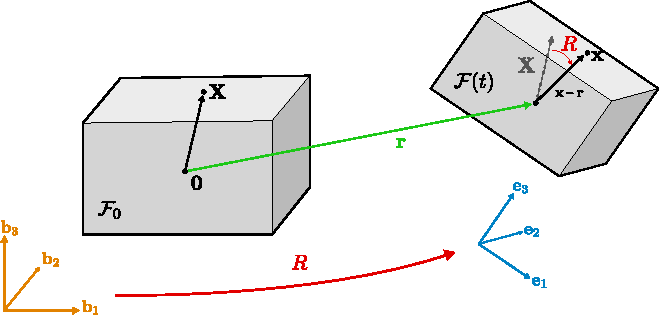
\includegraphics[width=0.8\textwidth]{figs_part2/sec3.1_introduction/rigid_body_kinematics.pdf}
        \caption{Illustration of the mapping from the reference configuration $\mathcal{F}_0$ to the current configuration $\mathcal{F}(t)$ of a rigid body. The configuration of the rigid body is specified via a translation of the center-of-mass $\mathbf{r}$ (green), and rotation $R$ (red), relative to a reference configuration with a center-of-mass located at $\mathbf{0}$. Material points $\mathbf{X}$ in the reference configuration are thus mapped to $\mathbf{x}(\mathbf{X}) = \mathbf{r} + R \mathbf{X}$. An observer that sits on the rigid body and moves with it will have a frame $E = (\mathbf{e}_1\ \mathbf{e}_2\ \mathbf{e}_3)$ (blue), which rotates relative to the fixed frame of a still observer $B = (\mathbf{b}_1\ \mathbf{b}_2\ \mathbf{b}_3)$ (orange) as $E = RB$.}
        \label{fig:rigid body kinematics}
\end{figure}

At time $t$ the location of the material point at $\mathbf{X}$ is given by $\mathbf{x}(\mathbf{X}, t)$. The latter can be related to the former as
\begin{equation} \label{eq:rigid body movement}
\mathbf{x}(\mathbf{X}, t) = \mathbf{r}(t) + R(t) \mathbf{X}, \quad  \mathbf{X} \in \mathscr{M}
\end{equation}
where $\mathbf{r}(t)$ is the location of the centre-of-mass and $R(t)$ is the rotation of the rigid body relative to its reference configuration. Now consider the second term in Eq. \ref{eq:rigid body movement},
\begin{equation}
R \mathbf{X} = \tilde{X}_i \mathbf{e}_i
\end{equation}
where $\mathbf{e}_i = R \mathbf{b}_i$ is the \textit{moving} or \textit{body} frame, which we write as $E = (\mathbf{e}_1\ \mathbf{e}_2\ \mathbf{e}_3) \in \mathbb{R}^{3 \times 3}$ and satisfies $E = RB$, and is illustrated in Fig.~\ref{fig:rigid body kinematics}. The configuration of the rigid body can thus be written as a matrix
\begin{equation}
\mathcal{F}(t) = \begin{pmatrix}
1 & \mathbf{0}^T \\
\mathbf{r}(t) & E(t)
\end{pmatrix}
\end{equation}
and we can relate it to the reference configuration as
\begin{equation}
\mathcal{F}(t) = \mathcal{F}_0  \Phi(t)
\end{equation}
where
\begin{equation}
\mathcal{F}_0 = \begin{pmatrix}
1 & \mathbf{0}^T \\
\mathbf{0} & B
\end{pmatrix}
\end{equation}
is the reference configuration and
\begin{equation} \label{eq:rigid body SE(3) state}
\Phi(t) = \begin{pmatrix}
1 & \mathbf{0}^T \\
B^T \mathbf{r} & B^T R(t) B
\end{pmatrix}
\end{equation}
is for each $t \in [0, T]$ an element of the special Euclidean group $SE(3)$ of translations and rotations. We will thus henceforth identify the configuration of the rigid body with $\Phi$, up to a global rotation of $\mathcal{F}_0$. 

The form of Eq.~\ref{eq:rigid body SE(3) state} merits some explanation. $B^T \mathbf{r}$ can be seen as the component of coefficients of $\mathbf{r}$ expressed in the fixed frame $B$, and $B^T R B$ is then the rotation $R$ in that same basis. We therefore introduce the notation $\tilde{v} = B^T \mathbf{v}$ for vectors $\mathbf{v} \in \mathbb{R}^3$. Similarly we write
\begin{equation}
\vec{v} = E^T \mathbf{v}
\end{equation}
where $\vec{v}$ is a vector $\mathbf{v} \in \mathbb{R}^3$ expressed in the moving frame $E$, with components $v_i = \mathbf{e}_i \cdot \mathbf{v}$. We thus have that $\mathbf{v} = v_i \mathbf{e}_i = \tilde{v}_i \mathbf{d}_i$.

We now derive the kinematic equations of motion of the rigid body, parametrised as a point $\Phi(t)$ in the Lie group $SE(3)$. The `velocity' of the rigid body is $\dot{\Phi}(t) \in T_{\Phi(t)} SE(3)$, a vector in the tangent space at $\Phi(t)$, which incorporates both the translation of the centre-of-mass and the rotation of the frame. As $SE(3)$ is a Lie group, there is a natural map from $T_{\Phi(t)} SE(3)$ to its Lie algebra $\mathfrak{se}(3) \cong T_{e} SE(3)$ by left (or right)-translation
\begin{equation} \label{eq:kinematics of rigid body}
\Phi^{-1} \dot{\Phi} = N \in \mathfrak{se}(3)
\end{equation}
which allows us to express the kinematics of the rigid body in terms of generalised velocities all taking values in the same Lie algebra. Equation \ref{eq:kinematics of rigid body} is an ordinary matrix differential equation and can be solved to find $\Phi(t)$ given a velocity $Y(t)$. 

We now derive the kinematic equations of motion of the rigid body in terms of more familiar quantities. Let $\vec{V}$ be the translational velocity of the center-of-mass, and $\vec{\Omega}$ the angular velocity of the rigid body, expressed in the moving frame basis. We write $N$ as
\begin{equation} \label{eq:rigid body Y}
N = \begin{pmatrix}
0 & \vec{0}^T \\
\vec{V} & \hat{\Omega}
\end{pmatrix}
\end{equation}
where $\hat{\Omega} \in \mathfrak{so}(3)$ is the angular velocity under the hat-map Eq.~\ref{eq:hat map}, which is the isomorphism between $3$-vectors and $3 \times 3$ antisymmetric matrices, and where $\mathfrak{so}(3)$ is the Lie algebra of the special orthogonal group $SO(3)$. We can see $N$ as a generalised velocity, defined on the Lie algebra. The inverse of Eq.~\ref{eq:rigid body SE(3) state} is given by
\begin{equation}
\Phi^{-1} = \begin{pmatrix}
1 & \mathbf{0}^T \\
-B^T R^T \mathbf{r} & B^T R^T B
\end{pmatrix}.
\end{equation}
We now evaluate the left-hand side of Eq.~\ref{eq:kinematics of rigid body} to get
\begin{equation} \label{eq:ginv g}
\begin{aligned}
\Phi^{-1} \dot{\Phi} = \mathcal{F}^{-1} \dot{\mathcal{F}} & = \begin{pmatrix}
  0 & \vec{0}^T \\
  B^T R^T \dot{\mathbf{r}} & B^T R^T \dot{R} B
\end{pmatrix} \\
& = \begin{pmatrix}
  0 & \vec{0}^T \\
  E^T \dot{\mathbf{r}} &  E^T \dot{E} 
\end{pmatrix}
\end{aligned}
\end{equation}
Equating Eq.~\ref{eq:rigid body Y} and Eq.~\ref{eq:ginv g}, we get the kinematic equations of motion
\begin{subequations}
\begin{align}
\dot{\mathbf{r}} & = \mathbf{V} \\
\dot{E} & = E \hat{\Omega}. \label{eq:frame eom}
\end{align}
\end{subequations}
which describes the translational motion of the centre-of-mass and the rotation of the frame $E$, respectively. Equation \ref{eq:frame eom} can also be written as
\begin{equation} \label{eq:e eom rigid body}
\begin{aligned}
\dot{\mathbf{e}}_j & = \mathbf{e}_i \hat{\Omega}_{ij} \\
& = \boldsymbol{\Omega} \times \mathbf{e}_i.
\end{aligned} 
\end{equation}
where $\boldsymbol{\Omega} = \Omega_i \mathbf{e}_i$. Eq.~\ref{eq:e eom rigid body} provides a clear interpretation of the angular velocity. At time $t$ the $i$th component of the angular velocity  in the moving frame $\Omega_i(t)$ gives the rate at which the rigid body rotates around the axis $\mathbf{e}_i$.

We note that the derivations above would simplify to some extent if we let the fixed frame equal the identity matrix $B=\mathbbm{1}$, in which case $E = R$. In this section we will keep the distinction so as to make the distinction clear between the moving frame $E$ and the fixed frame $B$. It is clear that $\mathcal{F}$ (and $\mathcal{F}_0$) could also be considered Lie group-valued, and indeed $\Phi^{-1} \dot{\Phi} = \mathcal{F}^{-1} \dot{\mathcal{F}}$. In the subsequent section we will make this identification.

Now we will consider the dynamics of the rigid body. We will start with the Euler-Lagrange equations defined on the Lie group, and then show the corresponding action principle defined on the Lie algebra. The kinetic energy of the rigid body is given by
\begin{equation}  \label{eq:rigid body kinetic energy}
\begin{aligned}
\mathcal{K}(\dot{\Phi}) & = \frac{1}{2} \int_\mathscr{M} \rho^V_0(\mathbf{X}) |\dot{\mathbf{x}}(\mathbf{X})|^2  d^3 X
\end{aligned}
\end{equation}
which is here written explicitly as a function of $\dot{\Phi}$. To see this note that
\begin{equation}
\begin{pmatrix} 1 \\ \mathbf{x} \end{pmatrix} = \mathcal{F}_0 \Phi \mathcal{F}_0^{-1} \begin{pmatrix} 1 \\ \mathbf{X} \end{pmatrix}
\end{equation}
and so $\mathbf{x}$ can be seen as a function of $\Phi$. The dynamical equations of motions of a free rigid body with Lagrangian density $L : SE(3) \times TSE(3) \to \mathbb{R}$
\begin{equation}
\mathcal{L}(\Phi, \dot{\Phi}) = \mathcal{K}(\dot{\Phi})
\end{equation}
are found by invoking \textit{Hamilton's principle}
\begin{equation} \label{eq:rigid body hamiltons principle}
\delta \int_0^{T} \mathcal{L}(\Phi(t), \dot{\Phi}(t)) dt = 0
\end{equation}
under variations $\Phi(t) \to \Phi(t) + \delta \Phi (t)$, where $\delta \Phi (t)$ is a variational test function which must vanish at the temporal boundaries, and where $T$ is the upper-bound of the time-domain considered. The resulting equations of motion will be second-order equations for $\Phi$ in time. This formulation is often undesirable, as in numerical simulations errors accrue such as to push $\Phi$ out of the sub-manifold $SE(3) \subset \mathbb{R}^{4 \times 4}$. We will next formulate the corresponding equations of motion on the Lie algebra instead.

%under variations $\Phi(t) \to \Phi(t) + \delta \Phi (t)$, where $\delta \Phi (t)$ is a variational test function which must vanish at the temporal boundaries, and where $T$ is the upper-bound of the time-domain considered. The resulting equations of motion are the \textit{Euler-Lagrange} equations
%\begin{equation} \label{eq:EL equations for g}
%\frac{\partial L}{\partial \Phi_{ij}} - \frac{d}{dt} \frac{\partial L}{\partial %\dot{\Phi}_{ij}} = 0, \quad i,j=1,\dots,4.
%\end{equation}
%As a consequence of the fact that Eq.~\ref{eq:EL equations for g} is formulated directly on the Lie group, the equation is explicitly $16$-dimensional, despite the fact that $\Phi(t) \in SE(3)$ and $\text{dim}(SE(3)) = 6$. This formulation is often undesirable, as in numerical simulations this leads to errors accruing such as to push $\Phi$ out of the sub-manifold $SE(3) \subset \mathbb{R}^{4 \times 4}$. We will next formulate the corresponding equations of motion on the Lie algebra.

We have that
\begin{equation} \label{eq:rigid body kinetic energy 2}
\begin{aligned}
\mathcal{K}(\dot{\Phi}) & = \frac{1}{2} m |\dot{\mathbf{r}}|^2 + \frac{1}{2} \int_\mathscr{M} \rho^V_0(\mathbf{X}) | \dot{R} \mathbf{X}|^2 d^3 X
\end{aligned}
\end{equation}
where we have used that $\int_M \rho^V_0(\mathbf{X}) \mathbf{X} d^3 X = 0$. Now, since
\begin{equation}
\begin{aligned}
|\dot{R} \mathbf{X}| & = |\dot{E} B^T X| = |\dot{E} \tilde{X}| = |E^T \dot{E} \tilde{X}|
= |\hat{\Omega} \tilde{X}| = |\vec{\Omega} \times \tilde{X}|
\end{aligned}
\end{equation}
we see that the rotational kinetic energy is a quadratic form in terms of the angular velocity $\vec{\Omega}$. Furthermore, as $|\dot{\mathbf{r}}| = |\vec{V}|$ we can write
\begin{equation} \label{eq:K lie algebra}
\begin{aligned}
\mathcal{K}(N) & = \frac{1}{2} m |\vec{V}|^2 + \frac{1}{2} \vec{\Omega}^T \mathbb{I} \vec{\Omega}
\end{aligned}
\end{equation}
where $\mathbb{I} \in \mathbb{R}^{3 \times 3}$ is the \textit{moment of inertia} tensor, which is, unless the body is incidental to a line, positive-definite. Eq.~\ref{eq:K lie algebra} is now a function of the Lie algebra-valued $N \in \mathfrak{se}(3)$. We define the \textit{reduced Lagrangian density} $\ell : \mathfrak{se}(3) \to \mathbb{R}$
\begin{equation}
\ell(N) = \mathcal{K}(N)
\end{equation}
which coincides with the regular Lagrangian density $\mathcal{L}(\Phi, \dot{\Phi}) = \ell(N)$ when $\Phi^{-1} \dot{\Phi} = N$. To find the corresponding Hamilton's principle
\begin{equation} \label{eq:lie algebra Hamiltons principle}
\delta \int_0^T \ell(N) dt = 0
\end{equation}
defined on the Lie algebra, we identify the space of admissible variations $\delta N$ in terms of the variations on the Lie group-level $\delta \Phi$. We vary Eq.~\ref{eq:kinematics of rigid body} to find
\begin{equation}
\begin{aligned}
\delta N = - \Phi^{-1} \delta \Phi \Phi^{-1} \dot{\Phi} + \Phi^{-1} \delta \dot{\Phi}.
\end{aligned}
\end{equation}
where we used $\delta (\Phi \Phi^{-1}) = 0$ to find $\delta \Phi^{-1}$. We define the variational test function $\eta = \Phi^{-1} \delta \Phi$, which satisfies $\dot{\eta} = - N \eta + \Phi^{-1} \delta \dot{\Phi}$. We get
\begin{equation} \label{eq:lie algebra variation}
\begin{aligned}
\delta N & = \dot{\eta} + [N, \eta] \\
& = \dot{\eta} + \text{ad}_N \eta.
\end{aligned}
\end{equation}
As we will compute the corresponding variational principle for the Cosserat rod in the subsequent section, we will not go through the detailed derivation here. If the variation Eq.~\ref{eq:lie algebra Hamiltons principle} is computed using Eq.~\ref{eq:lie algebra variation}, the resulting equations of motion are
\begin{equation} \label{eq:euler poincare equation for rigid body}
\frac{d}{dt} \frac{\partial \ell}{\partial N} = \text{ad}_N^* \frac{\partial \ell}{\partial N}
\end{equation}
where $\text{ad}^*_N : \mathfrak{se}(3)^* \to \mathfrak{se}(3)^*$ is the dual of the adjoint action, defined on the dual $\mathfrak{se}(3)^*$ to the Lie algebra, and $\frac{\partial \ell}{\partial N}$ is the matrix partial derivative which is carried out as in Eq.~\ref{eq:numerator-layout convention}. Equation \ref{eq:euler poincare equation for rigid body} is the result of the \textit{Euler-Poincaré theorem} \citep{marleHenriPoincareNote2013a, marsdenIntroductionMechanicsSymmetry2013, poincareFormeNouvelleEquations1901}, and is also thus referred to as the \textit{Euler-Poincaré equation}. Further details, and its derivation in the continuum case, will follow in the subsequent sections. Evaluating Eq.~\ref{eq:euler poincare equation for rigid body} leads to
\begin{subequations} \label{eq:dynamic eoms for rigid body}
\begin{align} 
\dot{\vec{V}} & = \vec{V} \times \vec{\Omega} \label{eq:V rigid body equation} \\
\mathbb{I} \dot{\vec{\Omega}} & = \mathbb{I} \vec{\Omega} \times \vec{\Omega}.
\end{align}
\end{subequations}
Eq.~\ref{eq:kinematics of rigid body} and Eq.~\ref{eq:dynamic eoms for rigid body} together fully specify the kinodynamics of the free rigid body respectively. Note that Eq.~\ref{eq:dynamic eoms for rigid body} is expressed in the moving frame, and reduces to $\dot{\mathbf{V}} = 0$ and $\dot{\boldsymbol{\Omega}} = 0$ in a non-moving frame.


%We note that Eq.~\ref{eq:rigid body kinetic energy 2} is invariant under left-translation by a rigid body transformation $\Psi = (\mathbf{t} ; \tilde{R} ) \in SE(3)$. Explicitly, we have
%\begin{equation}
%\begin{aligned}
%\mathcal{K}(\Psi \dot{\Phi}) & = \frac{1}{2} m | \tilde{R} \mathbf{r} + \mathbf{t} )|^2 + \frac{1}{2} \int_\mathscr{M} \rho^V_0(\mathbf{X}) | \tilde{R} \dot{R} \mathbf{X}|^2 d^3 X \\
%& = \frac{1}{2} m | \dot{\mathbf{r}} |^2 + \frac{1}{2} \int_\mathscr{M} \rho^V_0(\mathbf{X}) | \dot{R} \mathbf{X}|^2 d^3 X = \mathcal{K}(\dot{\Phi}).
%\end{aligned}
%\end{equation}
%The left-invariance of the kinetic energy entails that we can express it in terms of Lie algebraic quantities by setting $\Psi = \Phi^{-1}$.

We will now briefly consider the case of a rigid body under the influence of an external force. As the more general case of a continuum of rigid bodies will be treated in the following section, we will leave out many mathematical details, and only state some results here to preface the results that will follow.

External forcing of the rigid body can be included by considering the more general \textit{Lagrange-D'Alembert principle} \citep{marsdenIntroductionMechanicsSymmetry2013}, which is, in integral form
\begin{equation} \label{eq:integral lagrange-dalembert for rigid bodies}
\delta \int_0^T \mathcal{L}(\Phi, \dot{\Phi})\ dt + \int_0^T (\mathbf{T}(\Phi, \dot{\Phi}))( \delta \Phi ) dt = 0
\end{equation}
where $\mathcal{L}(\Phi, \dot{\Phi})$ is the Lagrangian density of the free rigid body, and $\mathbf{T} \in T^*SE(3)$ is a covector, where its argument is the variational test function $\delta \Phi$. $\mathbf{T}$ is here a generalised external force on the rigid body, containing both the force and the moment applied on the rigid body. As shown in \cite{wisniewskiEulerPoincarReductionExternally}, Eq.~\ref{eq:integral lagrange-dalembert for rigid bodies} in reduced form leads to
\begin{equation} \label{eq:reduced integral lagrange-dalembert for rigid bodies}
\delta \int_0^T \ell (N)\ dt + \int_0^T \langle T, \eta \rangle dt = 0
\end{equation}
where $T$ is the generalised external force pulled-back onto the dual Lie algebra $\mathfrak{se}(3)^*$, $\eta$ the variational test function defined on the Lie algebra, and $\langle \cdot , \cdot \rangle : \mathfrak{se}(3)^* \times \mathfrak{se}(3) \to \mathbb{R}$ is an inner product. If we let the $\vec{f}$ and $\vec{m}$ be the external force and moment respectively, the resulting equations of motion are
\begin{subequations} 
\begin{align} 
\dot{\vec{V}} & = \vec{V} \times \vec{\Omega} + \vec{f}  \\
\mathbb{I} \dot{\vec{\Omega}} & = \mathbb{I} \vec{\Omega} \times \vec{\Omega} + \vec{m}.
\end{align}
\end{subequations}
In the following section we will generalise these equations of motion for the Cosserat rod.

\section{Geometric Cosserat rod mechanics} \label{sec:Geometric Cosserat rod mechanics}

\subsection{Cosserat rod kinematics}

\begin{figure}[t]
\centering
        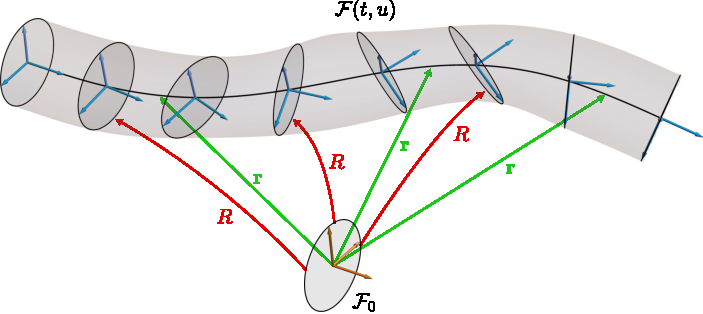
\includegraphics[width=0.8\textwidth]{figs_part2/sec7.2.1_cosserat_rod_kinematics/cosserat_F0_to_F.pdf}
        \caption{Illustration of the mapping from the reference configuration $\mathcal{F}_0$ to the current configuration $\mathcal{F}(u)$ of a Cosserat rod. The configuration of a Cosserat rod is specified by the center-line $\mathbf{r}(u),\ u \in [0, L_0]$ and a rigid body cross section attached at each $u$, related to a reference configuration $\mathcal{F}_0$, via translation (red) and rotation (red) respectively.}
        \label{fig:cosserat F0 to F}
\end{figure}

General Cosserat media can be described as a micros-tructured sub-manifold of Euclidean space. At each point-continua on the sub-manifold $n$ directors are attached, where each director can in general vary in both magnitude and direction independently. The \textit{special Cosserat rod} is an example of a Cosserat system where the one-dimensional continuum body is called the \textit{center-line} $\mathbf{r}(u)$, with two orthogonal directors at each material point $u \in [0, L_0]$, where $L_0$ is the rest length of the rod, that are constrained to be \textit{inextensible} (constant magnitude) and orthogonal. Equivalently, we can thus see the special Cosserat rod as a connected string of rigid body cross-sections. These cross-sections are represented as orthonormal frames we call the \textit{material frames} $E(u) = (\mathbf{e}_1(u)\ \mathbf{e}_2(u)\ \mathbf{e}_3(u))$, which rotate relative to each other along the material coordinate $u$. A pair $\mathbf{r}(u), E(u))$ is known as a \textit{trihedron}. See Fig.~\ref{fig:Cosserat kinematic degrees of freedom} for an illustration.

We will show that the kinematic configuration space of the Cosserat rod is the Lie group of special Euclidean transformations $SE(3)$, and then proceed to formulate its kinematic equations of motion on the corresponding Lie algebra $\mathfrak{se}(3)$.

\subsubsection*{Lie group–Lie algebra correspondence} \label{sec:Lie group–Lie algebra correspondence}

The center-of-mass of the cross-section at $u$ is given by $\mathbf{r}(u)$, and its orientation is specified by the material frame $E(u) = (\mathbf{e}_1(u)\ \mathbf{e}_2(u)\ \mathbf{e}_3(u))$, which is an orthonormal triad. As $E$ is a basis for $\mathbb{E}^3$, the vector of components in the material frame basis $\vec{v} = E^T \mathbf{v}$ will be said to be expressed in the \textit{moving frame}. The configuration of the Cosserat rod is thus specified by the center-line and material frame, which we write as
\begin{equation}
\mathcal{F}(t, u) = \begin{pmatrix}
1 & \mathbf{0}^T \\
\mathbf{r}(t, u) & E(t, u).
\end{pmatrix}
\end{equation}
We can relate rod configurations to a reference coordinate system as
\begin{equation} \label{eq:Cosserat rod from phi}
\mathcal{F}(t, u) = \mathcal{F}_0  \Phi(t, u)
\end{equation}
where
\begin{equation}
\mathcal{F}_0 = \begin{pmatrix}
1 & \mathbf{0}^T \\
\mathbf{0} & B
\end{pmatrix}
\end{equation}
is the reference coordinate system, and $\Phi(t,u) \in SE(3)$ is the transformation between the two. See Fig.~\ref{fig:cosserat F0 to F} for an illustration. In contrast the previous section, here we set the fixed frame to $B = \mathbbm{1}_{3 \times 3}$, to simplify the notation. Such that $\mathcal{F}_0 = \mathbbm{1}_{4 \times 4}$ and
\begin{equation} \label{eq:cosserat rod SE(3) state}
\Phi(t, u) = (\mathbf{r} ; E) = \begin{pmatrix}
1 & \mathbf{0}^T \\
\mathbf{r}(t,u) & E(t,u) 
\end{pmatrix} \in SE(3).
\end{equation}
where we have introduced the short-hand notation for $\Phi = (\mathbf{r} ; E)$ for $SE(3)$ elements. We thus have that $\mathcal{F}(t,u) = \Phi(t,u)$, and we will henceforth identify the Cosserat rod configuration with the group element $\Phi(t,u)$. The kinematic motion of the Cosserat rod can thus be fully specified by a space-time sheet $\Phi(t, u) \in SE(3)$ in the Lie group of special Euclidean transformations. In other words, the spatio-temporal configuration of the Cosserat rod can be described as a $2$-dimensional immersion $N \subset SE(3)$, defined by the map $\Phi : W \to SE(3)$, where we call $W = [0, T] \times [0, L_0]$ the \textit{kinematic base space}, and $N = \Phi(W)$. Therefore we call $SE(3)$ the \textit{kinematic configuration space} of the Cosserat rod, and $\Phi$ the \textit{spatio-temporal configuration} of the system. In other words, $N$ can be seen as a `sheet' in $SE(3)$, and is parametrised by the function $\Phi$. The manifolds $[0, L_0]$ and $[0, T]$ will be called the \textit{material base space} and the \textit{time domain} respectively. Furthermore, we may draw a distinction between the \textit{internal configuration space} $SO(3)$, corresponding to the material frame, and the \textit{external configuration space} $\mathbb{E}^3 \cong SE(3) / SO(3)$, corresponding to the center-line.

At a point $\Phi(t, u) \in N$, we can consider velocities in the temporal and spatial directions $\dot{\Phi}(t, u)$ and $\Phi'(t, u)$ respectively. Thus by differentiating the map $\Phi$ we get a vector field
\begin{equation}
d\Phi = \dot{\Phi} dt + \Phi' du
\end{equation}
as discussed in Sec.~\ref{sec:The Maurer-Cartan form}, where $d \Phi(t, u) \in T_{\Phi(t, u)} N$ for all $(t, u) \in W$. Here it is worth clarifying a technical point to avoid confusion. Although we say $d \Phi$ is a vector field on $N$, we have written it as a $1$-form on the kinematic base space $W$. These two notions are not contradictory. Precisely, $d\Phi$ is a \textit{$TN$-valued $1$-form on $W$}.

Via left-translation, we can relate $d \Phi$ to a $\mathfrak{se}(3)$-valued $1$-form on $W$
\begin{equation} \label{eq:xi from phi}
\xi = \Phi^{-1} d \Phi
\end{equation}
where $\xi = \Phi^* \omega$, the pull-back $\Phi^* \omega$ of the Maurer-Cartan $\omega$ form, as discussed in Sec.~\ref{sec:Sub-manifolds of homogeneous spaces}. $\xi$ contains all geometric information contained in $\Phi$, up to rigid body transformations, and as a Lie algebra-valued object $\xi$ will turn out to be easier to work with than $\Phi$ or $d \Phi$. In what follows, we will formulate the kinematics of the Cosserat rod entirely within the Lie algebra using $\xi$.

\subsubsection*{Kinematic equations of motion}

Equation \ref{eq:xi from phi} shows how to construct $\xi$ from the Lie group function $\Phi$. For our purposes it will be more relevant to go the other direction: Given a $\xi$, is there a corresponding $\Phi$? The answer can be formulated in terms of integrability. As a motivating and intuitive example from multi-variate calculus, consider a vector-valued function $\mathbf{F} : \mathbb{R}^3 \to \mathbb{R}^3$. There exists a potential $U : \mathbb{R}^3 \to \mathbb{R}$ such that $\mathbf{F} = - \nabla \cdot U$ if and only if the differential $\phi = \frac{\partial F_i}{\partial x^i} dx^i$ is \textit{exact}. In $\mathbb{R}^3$, and for Lie groups, this is equivalent to $d \phi = 0$ \footnote{This is known as the \textit{Poincaré lemma} and holds true locally for arbitrary manifolds.}. In Sec.~\ref{sec:Sub-manifolds of homogeneous spaces}, we showed that there is a $\Phi$ for which the right-hand side of Eq.~\ref{eq:xi from phi} holds true if and only if
\begin{equation} \label{eq:xi integrability condition}
d\xi + \xi \wedge \xi = 0.
\end{equation}
This is an integrability condition on $\xi$, and is a Maurer-Cartan equation on the sub-manifold $N$. As we will show, Eq.~\ref{eq:xi integrability condition} is in fact a concise expression of the kinematics of a Cosserat rod. We expand $\xi$ in terms of its temporal and spatial components
\begin{equation} \label{eq:xi = X + N}
\xi = N dt + X du
\end{equation}
where $X(t, u), N(t, u) \in \mathfrak{se}(3)$, which we write as
\begin{subequations} \label{eq:X and Y defs}
\begin{align}
X & = \{ \vec{\theta} ; \vec{\pi} \} =  \begin{pmatrix}
	0 & \vec{0}^T \\
	\vec{\theta} & \hat{\pi} 
\end{pmatrix} \label{eq:X def} \\ 
N & = \{ \vec{V} ; \vec{\Omega} \} = \begin{pmatrix}
	0 & \vec{0}^T \\
	\vec{V} & \hat{\Omega} 
\end{pmatrix}
\end{align}
\end{subequations}
where $\vec{\theta}(t,u), \vec{\pi}(t,u), \vec{V}(t,u), \vec{\Omega}(t,u) \in \mathbb{R}^3$ are vectors expressed in the material frame basis, and where we have introduced the notation $X = \{ \vec{\theta} ; \vec{\pi} \}$ as a shorthand for matrices like Eq.~\ref{eq:X def}. We will call $X$ the \textit{spatial reconstruction field} and $N$ the \textit{generalised velocity field}. Following a similar derivation as in Eq.~\ref{eq:ginv g}, we find
\begin{equation}
\Phi^{-1} d \Phi = \begin{pmatrix}
0 & \vec{0}^T \\
E^T d \mathbf{r} & E^T d E
\end{pmatrix}.
\end{equation}
\begin{figure}[t]
\centering
        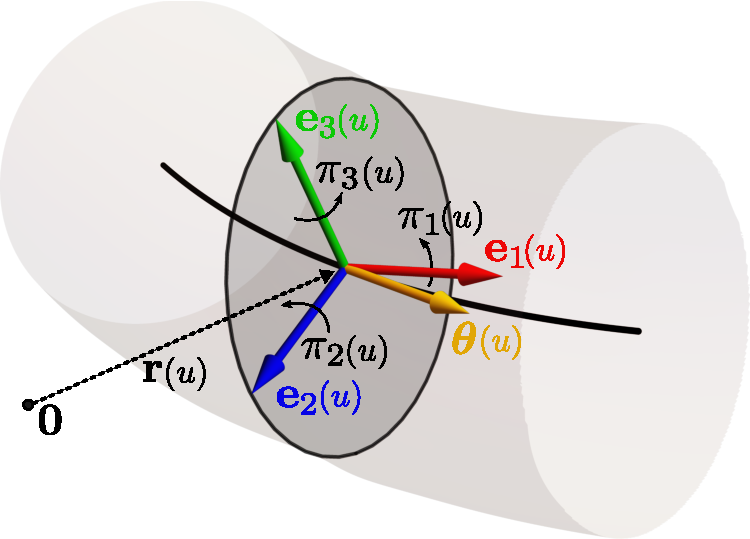
\includegraphics[width=0.65\textwidth]{figs_part2/sec7.2.1_cosserat_rod_kinematics/theta_and_pi_explanation.pdf}
        \caption{Depicts the rate-of-change along $u$ of the material frame located at $\mathbf{r}(u)$ (dashed line). The spatial derivative of the center-line (solid black line) at $u$ is $\boldsymbol{\theta}(u) = \mathbf{r}'(u)$ (yellow arrow), and $\pi_1$, $\pi_2$ and $\pi_3$ is the angular rate-of-change of the material frame around $\mathbf{e}_1$ (red), $\mathbf{e}_2$ (blue) and $\mathbf{e}_3$ (green) respectively. The analogous description holds true for $\vec{V}$ and $\vec{\Omega}$, but in time $t$ rather than material coordinate $u$.}
        \label{fig:rate-of-change of material frame}
\end{figure}
From Eq.~\ref{eq:X and Y defs} we then find that
\begin{subequations} \label{eq:dr and de}
\begin{align}
d \mathbf{r} & = \mathbf{e}_i V_i dt + \mathbf{e}_i \theta_i du \\
d \mathbf{e}_j & = \mathbf{e}_i \hat{\Omega}_{ij} dt + \mathbf{e}_i \hat{\pi}_{ij} du \label{eq:de_j}
\end{align}
\end{subequations}
which we can also write as
\begin{subequations}
\begin{align}
d \mathbf{r} & = \mathbf{V} dt + \boldsymbol{\theta} du \\
d E & = E \hat{\Omega} dt + E \hat{\pi} du. 
\end{align}
\end{subequations}
We can thus identify $\mathbf{V} = E \vec{V} = \partial_t \mathbf{r}$ as the translational velocity of the center-line, $\boldsymbol{\theta} = E \vec{\theta} = \partial_u \mathbf{r}$ as rate-of-change of the center-line along the material coordinate, and from Eq.~\ref{eq:de_j} it follows that
\begin{subequations}
\begin{align}
\dot{\mathbf{e}}_i & = \boldsymbol{\Omega} \times \mathbf{e}_i \\
\mathbf{e}_i' & = \boldsymbol{\pi} \times \mathbf{e}_i \label{eq:eom for e_i along u}
\end{align}
\end{subequations}
which show that $\boldsymbol{\Omega} = E \vec{\Omega}$ and $\boldsymbol{\pi} = E \vec{\pi}$ are the temporal and `spatial' angular velocities of the material frame respectively. The spatial part of Eq.\ref{eq:dr and de} is illustrated in Fig.~\ref{fig:rate-of-change of material frame}.  We can thus see $N$ as a generalised velocity in the Lie algebra. Equation \ref{eq:de_j} also shows how derivatives of vector functions $\mathbf{v}(t,u)$ can be expressed in terms of $\vec{v}(t,u)$ in the moving frame basis. We have
\begin{equation}
\begin{aligned}
d \mathbf{v} & = d(\mathbf{e}_i v_i) \\
& = \mathbf{e}_i (d v_i) + (d \mathbf{e}_i) v_i \\
& = E (d \vec{v}) + (E \hat{\pi} + E \hat{\Omega}) v_i \\
& = E (D_t \vec{v}\ dt + D_u \vec{v}\ du) 
\end{aligned}
\end{equation}
such that $E^T d \mathbf{v} = D_u \vec{v}\ du + D_t \vec{v}\ dt$, where
\begin{subequations} \label{eq:covariant derivatives}
\begin{align}
D_t & = \partial_t + \hat{\Omega}  \\
D_u & = \partial_u + \hat{\pi} 
\end{align}
\end{subequations}
are the spatial and temporal \textit{material derivatives} respectively. We thus have that $E^T \mathbf{v}' = D_u \vec{v}$  and $E^T \dot{\mathbf{v}} = D_t \vec{v}$.

For a given spatio-temporal velocity field $N(t,u)$, Eq.~\ref{eq:xi integrability condition} imposes a condition on the spatial reconstruction field $X(t,u)$. The resulting equations are the kinematic equations of motion. Substituting Eq.~\ref{eq:xi = X + N} into the left-hand side of Eq.~\ref{eq:xi integrability condition}
\begin{equation}
\begin{aligned}
d \xi + \xi \wedge \xi & = N' dt \wedge du + \dot{X} dt \wedge du + X N dt \wedge du  + N X dt \wedge du \\ 
& = (\dot{X} - N' + [N, X]) dt \wedge du,
\end{aligned}
\end{equation}
we get
\begin{equation} \label{eq:kinematic equations of motion in the Lie algebra}
\dot{X} = \mathcal{D}_u N.
\end{equation}
where we have defined
\begin{equation}
\mathcal{D}_u = \partial_u + \text{ad}_X
\end{equation}
which we will call a \textit{generalised material derivative}. Equation \ref{eq:kinematic equations of motion in the Lie algebra} is the kinematic equation of motion for the Cosserat rod, which expresses the evolution of the spatial configuration $X$, in terms of the generalised velocity $N$. To express the kinematics in terms of the non-generalised velocities, we substitute Eq.~\ref{eq:X and Y defs} into Eq.~\ref{eq:kinematic equations of motion in the Lie algebra} to find
\begin{subequations} \label{eq:kinematic equations of motion in the moving frame}
\begin{align}
D_t \vec{\theta} & = D_u \vec{V} \\
\partial_t \vec{\pi} & = D_u \vec{\Omega}, \label{eq:pi eom}
\end{align}
\end{subequations}
which are equivalent to Eq.~\ref{eq:kinematic equations of motion in the Lie algebra} and are the kinematic equations of motion expressed in the moving frame. At the Lie group-level the corresponding equations are
\begin{subequations} \label{eq:kinematic equations of motion in the fixed frame}
\begin{align}
\dot{\mathbf{r}} & = \mathbf{V} \\
\dot{\mathbf{e}}_i & = \boldsymbol{\Omega} \times \mathbf{e}_i \label{eq:e_i eom}
\end{align}
\end{subequations} % \dot{\boldsymbol{\pi}} & = \boldsymbol{\Omega}' + \boldsymbol{\Omega} \times \boldsymbol{\pi}.
From the numerical standpoint, the benefit of Eq.~\ref{eq:pi eom} over  Eq.~\ref{eq:e_i eom} is clear. Errors in integrating the latter can in general lead to $|\mathbf{e}_i| \neq 1$ and $\mathbf{e}_i \cdot \mathbf{e}_j \neq 0$, whilst by errors in Eq.~\ref{eq:pi eom} are by construction Lie algebra-valued. In other words, errors in Eq.~\ref{eq:e_i eom} accrue in $\mathbb{R}^{3 \times 3}$, whilst errors in Eq.~\ref{eq:pi eom} accrue within the Lie group itself. Mathematically, this is due to the fact that Eq.~\ref{eq:kinematic equations of motion in the Lie algebra} is defined on the linear space $W \times \mathfrak{se}(3)$, as opposed to Eq.~\ref{eq:kinematic equations of motion in the fixed frame} which is defined on the non-linear space $G \times TG$.

\subsubsection*{Types of deformations} \label{sec:deformation types}

Fig.~\ref{fig:Examples of Cosserat deformations} shows the various types of deformations that are kinematically possible for the Cosserat rod. Here we will describe how these deformations are encoded in $\vec{\theta}$ and $\vec{\pi}$. Since $\boldsymbol{\theta} = \mathbf{r}'$ we have that if $\vec{\theta}(u) \propto (1\ 0\ 0)$ then the material frame at $u$, pointing in the direction $\mathbf{e}_1(u)$ is aligned with the center-line. We thus see that $\vec{\theta}$ measures the \textit{shear} of the rod. Note that this is because $\vec{\theta}$ is expressed in the moving frame; $\boldsymbol{\theta}$ does not contain any information about the shear.

\textit{Twist} is the rotation of the material frame around $\mathbf{e}_1$, and the rate of twist along the material coordinate is given by $\pi_1$. Similarly, the rotation of the material frame around $\mathbf{e}_2$ and $\mathbf{e}_3$ are given by $\pi_2$ and $\pi_3$ respectively, as depicted in Fig.~\ref{fig:rate-of-change of material frame}.

In a non-moving frame the \textit{bending} of the center-line is encoded in $\mathbf{r}$, likewise $\boldsymbol{\theta}$. In the moving frame it is encoded in both $\vec{\theta}$ and $\vec{\pi}$ simultaneously. For instance, is $\vec{\theta}$ is constant along $u$ and $\pi_2$ or $\pi_3$ are non-zero along $u$, then the rod is bending.

In general velocities $\vec{V}$ will cause the Cosserat to \textit{extend}. Locally, the extension is described by the scalar $h(u) =  \left| \mathbf{r}' \right| = |\vec{\theta}|$, which can be seen as the square root of the metric on the center-line induced by the Euclidean metric on $\mathbb{R}^3$. Using $h$ we can define an arc-length coordinate as
\begin{equation}
ds = h(u) du
\end{equation}
which relates the arc-length increment $ds$ to the material length increment $du$. In the arc-length parametrisation we thus have $ \left| \frac{\partial \mathbf{r}}{\partial s} \right| = 1$ for all $s \in [0, L]$ where
\begin{equation}
L[h(u)] = \int_0^{L_0} h(u) du
\end{equation}
is the total arc-length of the center-line. $h(u)$ thus measures the local extension of the rod, where $h(u) = |\vec{\theta}| = 1$ indicates that the rod is not suffering an extension at $u$.

We define a unit-vector tangent to the center-line $\mathbf{t} = \boldsymbol{\theta} / |\boldsymbol{\theta}|$. The \textit{curvature} of the center-line is then a scalar defined as
\begin{equation} \label{eq:scalar curvature}
\kappa = |\mathbf{t}'|.
\end{equation}
In the literature it is more common to define the curvature in terms of the arc-length parametrisation, which we write as $\tilde{\kappa} = |\partial_s \mathbf{t}| = |\partial_s^2 \mathbf{r}|$.

%In practice, for the aforementioned reasons on the benefits of working with Lie algebra-valued (rather than Lie group-valued) objects, we will use Eq.~\ref{eq:kinematic equations of motion in the Lie algebra} or Eq.~\ref{eq:kinematic equations of motion in the moving frame} rather than Eq.~\ref{eq:kinematic equations of motion in the fixed frame}.

%Although equivalent, it is important to note the practical and theoretical differences in integrating Eq.~\ref{eq:kinematic equations of motion in the fixed frame}, as compared to integrating Eq.~\ref{eq:kinematic equations of motion in the Lie algebra} or Eq.~\ref{eq:kinematic equations of motion in the moving frame}. In the latter, 

\subsubsection*{Reconstructing the Cosserat rod from $\xi$} \label{sec:reconstructing the cosserat rod}

Solving Eq.~\ref{eq:kinematic equations of motion in the Lie algebra}, for a given velocity $N$, yields the Lie algebra-valued $1$-form $\xi$ which contains, in infinitesimal form, information from which the Cosserat rod $\mathcal{F}$ can be reconstructed. Firstly, recall that we can reconstruct $\Phi$, the representation of the Cosserat rod as a space-time sheet in the Lie group, from $\xi$ using Eq.~\ref{eq:xi from phi}. Secondly, from Eq.~\ref{eq:Cosserat rod from phi} we note that $\Phi^{-1} d \Phi = \mathcal{F}^{-1} d \mathcal{F}$. Therefore we can reconstruct the Cosserat rod from $\xi$ by solving the equation
\begin{equation}
d \mathcal{F} = \mathcal{F} \xi.
\end{equation}
We will now put the above into a form solvable as a matrix ordinary differential equation. By expanding $\mathcal{F}^{-1} d \mathcal{F}$ into its components, and from Eq.~\ref{eq:xi = X + N} we find that
\begin{subequations} \label{eq:reconstruction of F eqs}
\begin{align}
\mathcal{F}^{-1} \mathcal{F}' & = X \label{eq:phi u matrix ode} \\
\mathcal{F}^{-1} \dot{\mathcal{F}} & = Y. \label{eq:phi t matrix ode}
\end{align}
\end{subequations}
For fixed $t = \bar{t}$ and given initial conditions Eq.~\ref{eq:phi u matrix ode} can be used to find $\mathcal{F}(u,\bar{t})$ for $u \in [0, L_0]$, and for fixed $u = \bar{u}$ and given initial conditions Eq.~\ref{eq:phi t matrix ode} can be used to find $\mathcal{F}(\bar{u}, t)$ for $t \in [0, T]$. We can therefore trace out and reconstruct $\mathcal{F}(t,u)$ by repeatedly solving Eqs.~\ref{eq:phi u matrix ode} and \ref{eq:phi t matrix ode}. Due to Eq.~\ref{eq:xi integrability condition}, which ensures that $d \mathcal{F}$ is an `exact' differential, the resulting $\mathcal{F}(t,u)$ is invariant with respect to the particular path in $(t,u)$-space taken to reconstruct it. Therefore, a suitable scheme to reconstruct $\mathcal{F}$ is to first reconstruct the Cosserat rod in time along $u=0$ by solving
\begin{equation} \label{eq:1st step reconstruction}
\bar{\mathcal{F}}(t) = \bar{\mathcal{F}}(t) \dot{\bar{\mathcal{F}}}(t),
\end{equation}
with initial condition $\bar{\mathcal{F}}(0) = \mathcal{F}^{0,0}$, where the latter corresponds to choosing values for $\mathbf{r}(0,0)$ and $E(0,0)$. Secondly, for any given time $t = \bar{t}$ we can reconstruct the Cosserat rod in space by solving
\begin{equation}
\mathcal{F}(u,\bar{t}) = \mathcal{F}(u, \bar{t}) \mathcal{F}(u, \bar{t})',
\end{equation}
with initial condition $\mathcal{F}(0, \bar{t}) = \bar{\mathcal{F}}(\bar{t})$. See App.~\ref{app:Reconstructing the Cosserat rod from xi} for a detailed description of the numerical algorithm.

\subsubsection*{Closed Cosserat rods}

Thus far we have considered $\textit{open}$ Cosserat rods, for which $\mathbf{r}(0) \neq \mathbf{r}(L_0)$ and $E(0) \neq E(L_0)$. For \textit{closed} Cosserat rods the material coordinate $u \in [0, L_0]$ is periodic in its domain, and the center-line and material frame must also be periodic and continuous in $u$. Although seemingly complicated, the following derivations fill result in showing that the case of a closed Cosserat can be in practice treated equivalently to an open Cosserat rod.

A closed rod implies that
\begin{equation} \label{eq:periodic X}
X(0) = X(L_0).
\end{equation}
However, Eq.~\ref{eq:periodic X} is only a necessary, but not sufficient, condition for the rod to close. The sufficient condition is for the constraint
\begin{equation}
\mathcal{F}(0, t) = \mathcal{F}(L_0, t)
\end{equation}
to hold for all $t$. This is an integral constraint on $X$, as formally we can write
\begin{equation}
\mathcal{F}(L_0, t) = \mathcal{F}(0, t) \mathscr{U} \exp \left\{ \int_0^{L_0} X du  \right\}
\end{equation}
where $\mathscr{U}$ denotes a $u$-ordered integral. The integral constrain on $X$ is therefore
\begin{equation} \label{eq:closed rod integral constraint}
\mathscr{U} \exp \left\{ \int_0^{L_0} X du  \right\} = \mathbbm{1}.
\end{equation}
However, if $N$ is a smooth function of $u$, the kinematic equations of motion will preserve Eq.~\ref{eq:closed rod integral constraint}. This means that if the rod is initialised to obey Eq.~\ref{eq:closed rod integral constraint} at $t=0$, it will continue to do so for all $t$.

In practice, in order to simulate a closed filament we must thus first construct on the Lie group-level a periodic $\mathcal{F}(u, 0)$, and then use Eq.~\ref{eq:phi u matrix ode} to find $X(u, 0)$ that obeys Eq.~\ref{eq:closed rod integral constraint}.

\subsection{Cosserat rod dynamics} \label{sec:Cosserat rod dynamics}

\subsubsection*{Constitutive dynamics} \label{sec:Cosserat rod constitutive dynamics}

Thus far we have considered the Cosserat rod abstractly as a sub-manifold of $SE(3)$. Physically, the Cosserat rod is a kinematic approximation of a deformable and slender tube. Let $\mathscr{M} = D \times [0, L_0] \subset \mathbb{R}^3$ be the reference configuration of such a tube, where $D \subset \mathbb{R}^2$ is the cross-section of the tube and is of arbitrary shape. Let $\mathbf{X} \in \mathscr{M}$ denote the material coordinates of $\mathscr{M}$, such that $X_1 \in [0, L_0]$ and $(X_2, X_3) \in \mathscr{D}$ and for simplicity let $\rho^V_0$ be a constant mass density per unit material volume at each $\mathbf{X}$. At time $t$ the location of the material point at $\mathbf{X}$ is given by $\mathbf{x}(\mathbf{X}, t)$, which are the deformed coordinates. We define $(X_2, X_3)$ to be in the centre-of-mass of the cross-section, such that $\int_{\mathscr{D}} X_\gamma d X_2 d X_3 = 0,\ \gamma = 2,3$.

The Cosserat rod models the slender deformable tube under the kinematic assumption that the material fibres that run radially from the center of $\mathcal{D}$ to its edge are fixed. In other words we impose that
\begin{equation} \label{eq:cosserat rod kinematic assumption}
\mathbf{x}(\mathbf{X}, t) = \mathbf{r}(t, u) + X_\gamma \mathbf{e}_\gamma(t, u), \quad \gamma = 2,3
\end{equation}
where $\mathbf{r}(t, u)$ is the center-line of the rod and where $u = X_1$ is the material coordinate along the center-line. The three-dimensional tube has thus been replaced with the Cosserat rod, which only has one spatial dimension. In this coarse-graining, the two missing spatial dimensions have been replaced by rigid body cross-sections attached at each $u \in [0, L_0]$, with orientation specified by the two directors $\mathbf{e}_2$ and $\mathbf{e}_3$.

As in Sec.~\ref{sec:Introduction - rigid body} we formulate the dynamics of the Cosserat rod via a Lagrangian formulation. We will again be using a reduction of the Lagrangian to construct dynamics defined on the Lie algebra. We derive the constitutive dynamics by first computing the kinetic energy of the rod in terms of its generalised velocity $N = \{ \vec{V} ; \vec{\Omega} \}$.

We assume that the dynamics is defined by a Lagrangian density of the form $\mathcal{L}(\Phi, d \Phi)$, and that its kinetic energy term is given by
\begin{equation} \label{eq:lagrangian of tube}
\int_0^{L_0} \mathcal{K}(\dot{\Phi})\ du = \frac{1}{2} \int_\mathscr{M} \rho^{V}_0 | \dot{\mathbf{x}} |^2\ d^3 X
\end{equation} 
where $\mathcal{K}$ is the kinetic energy density along the material coordinate $u$. Substituting in Eq.~\ref{eq:cosserat rod kinematic assumption} we get
\begin{equation} \label{eq:K intermediate result 1}
\int_0^{L_0} \mathcal{K}(\dot{\Phi})\ du = \frac{1}{2} \int_0^{L_0} \rho_0 |\mathbf{V}|^2 du + \frac{1}{2} \rho_0^V \int_\mathscr{M} \mathbf{V} \cdot \dot{\mathbf{e}}_\gamma X_\gamma d^3 X  + \frac{1}{2} \rho_0^V \int_\mathscr{M} |X_\gamma \dot{\mathbf{e}}_\gamma|^2 d^3 X
\end{equation} 
where $\rho_0 = A \rho^{V}_0$ is the mass density per unit material length, and $A = \int_D d X_2 dX_3$ is the area of the cross-section, and we have used $\dot{\mathbf{r}} = \mathbf{V}$. The second term in Eq.~\ref{eq:K intermediate result 1} vanishes when the integral over $D$ is evaluated. To evaluate the third term, let $\bar{\mathbf{X}} = X_\gamma \mathbf{e}_\gamma$, and note that $\mathbf{e}_i = \boldsymbol{\Omega} \times \mathbf{e}_i$, and so
\begin{equation}
|X_\gamma \dot{\mathbf{e}}_\gamma|^2 = |X_\gamma \boldsymbol{\Omega} \times \mathbf{e}_\gamma|^2 = |\boldsymbol{\Omega} \times \bar{\mathbf{X}}|^2 = |E (\vec{\Omega} \times \bar{\vec{X}})|^2 = |\vec{\Omega} \times \vec{\bar{X}}|^2
\end{equation}
where we used $(E\vec{\Omega}) \times (E\vec{\bar{X}}) = E (\vec{\Omega} \times \vec{\bar{X}})$. As $|(\vec{\Omega} \times \vec{\bar{X}})|^2$ is a quadratic form in $\vec{\Omega}$, we can write
\begin{equation}
\frac{1}{2} \rho_0^V \int_\mathscr{M} |X_\gamma \dot{\mathbf{e}}_\gamma|^2 d^3 X = \frac{1}{2} \int_0^{L_0} \vec{\Omega}^T \mathbb{I} \vec{\Omega} du
\end{equation}
where $\mathbb{I}$ is the cross-sectional moment-of-inertia per unit material length. We can thus write the kinetic energy of the Cosserat rod as $K(N) = \int_0^{L_0} \mathcal{K}(N) du$ where 
\begin{equation} \label{eq:reduced kinetic energy}
\mathcal{K}(N)  = \frac{1}{2} \rho_0 |\vec{V}|^2 +  \frac{1}{2} \vec{\Omega}^T \mathbb{I} \vec{\Omega}
\end{equation}
is the kinetic energy per material unit length, which is now explicitly a function of the generalised velocity $N$.

Having established that the kinetic energy of the Cosserat rod has a reduced form, we now assume that we have a reduced Lagrangian density of the form
\begin{equation} \label{eq:cosserat reduced lagrangian}
\ell(\xi) = \mathcal{K}(N) - \mathcal{U}(X)
\end{equation}
where $\mathcal{U}(X)$ is the potential energy per material unit length of a given spatial configuration $X = \{ \vec{\theta} ; \vec{\pi} \}$, and $\ell(\xi)$ is here a Lagrangian density defined on the Lie algebra. The reduced Lagrangian density satisfies $\ell(\xi) = \mathcal{L}(\Phi, d\Phi)$ when $\xi = \Phi^{-1} d \Phi$. 

The reduced Lagrangian density Eq.~\ref{eq:cosserat reduced lagrangian} is explicitly invariant under Galilean transformations, as it is written in terms of the invariant quantities $X$ and $N$. Physically, the fact that a Lagrangian $\mathcal{L}(\Phi, d\Phi)$ admits a reduction $\ell(\xi)$ entails that only differential deformations couple to the dynamics. In other words the Lagrangian is really only a function of the tangent space $\mathcal{L}(d \Phi)$. We will henceforth omit the argument in $\Phi$ when the Lagrangian density admits a reduced form.

%The Lagrangian formalism motivates the definition of a momentum, conjugate to the generalised velocity $Y$, which take values in the dual $\mathfrak{se}(3)^*$ to the Lie algebra $\mathfrak{so}(3)$. $\mathfrak{se}(3)^*$ is the space of linear operators on $\mathfrak{se}(3)$, and in matrix form can be written as \citep{fultonRepresentationTheoryFirst2013}
%\begin{equation}
%\mathfrak{se}(3)^* = \{ -A^T\ |\ A \in \mathfrak{se}(3) \}
%\end{equation}


The \textit{generalised conjugate momentum} of the Cosserat rod is
\begin{equation} \label{eq:generalised conjugate momentum def cosserat}
S := \frac{\partial \ell}{\partial N}  = \frac{\partial \mathcal{K}}{\partial N} = \begin{pmatrix}
0 & \vec{P}^T \\ 
\vec{0} & \hat{L}^T
\end{pmatrix}  \in \mathfrak{se}(3)^*
\end{equation}
where $\vec{P} = \rho_0 \vec{V}$ and $\vec{L} = \mathbb{I} \vec{\Omega}$. The matrix derivative is carried out using the numerator-layout convention Eq.~\ref{eq:numerator-layout convention}, such that $S_{ij} = \partial \ell /\partial N_{ji}$. The matrix representation of the dual Lie algebra can thus be seen as the space $\mathfrak{se}(3)^* = \{ Y^T\ :\ Y \in \mathfrak{se}(3) \}$. It will become clear that $\vec{P}$ is the linear momentum of the center-line per unit material length, and $\vec{L}$ is the angular momentum per unit material length of the material frame. We use the short-hand $S = \{ \vec{P} ; \vec{L} \}^*$, corresponding to matrices of the form Eq.~\ref{eq:generalised conjugate momentum def cosserat}. The matrix derivative $\frac{\partial \ell}{\partial N}$ is evaluated only with respect to the non-zero components of $N$, for which we have $S_{ji} = \frac{\partial \ell}{\partial N_{ij}}$, and $S_{ji} = 0$ otherwise. $S$ can be seen to take values in the dual Lie algebra $\mathfrak{se}(3)^*$, which is the space of linear operators $\mathfrak{se}(3) \to \mathbb{R}$ on the Lie algebra. To see this, note that $\mathcal{K}(N)$ can be written as
\begin{equation}
\mathcal{K}(N) = \frac{1}{2} \langle N, P \rangle
\end{equation}
where $\langle \cdot , \cdot \rangle : \mathfrak{se}(3) \times \mathfrak{se}(3)^* \to \mathbb{R}$ is an inner product defined as
\begin{equation}
\langle A , B \rangle =  \vec{a} \cdot \vec{b} + \vec{m} \cdot \vec{n}
\end{equation}
where $A = \{\vec{a}; \vec{m}\} \in \mathfrak{se}(3)$ and $B = \{\vec{b}; \vec{n}\} \in \mathfrak{se}(3)^*$. Similarly, we can define a \textit{generalised stress}, conjugate to the spatial configuration $X$, as
\begin{equation}
Q := \frac{\partial \mathcal{U}}{\partial X}.
\end{equation}
We write its components as $Q = \{ \vec{F} ; \vec{M} \}^*$ where
\begin{subequations} \label{eq:F_i and M_i from U}
\begin{align}
F_i = \frac{\partial \mathcal{U}}{\partial \theta_i} \\
M_i = \frac{\partial \mathcal{U}}{\partial \pi_i} 
\end{align}
\end{subequations}
are, as will be shown, the force on the center-line and the moment on the material frame respectively.

To find dynamic equations of motion for $P$ and $Q$, we invoke Hamilton's principle that variations
\begin{equation} \label{eq:variation of ell}
\delta \int_W \ell(\xi)\ dt \wedge du
\end{equation}
must vanish, where $\ell(\xi)$ is again the reduced Lagrangian density for the system. As for the rigid body in Sec.~\ref{sec:Introduction - rigid body}, we must first derive the permissible form of the variations. We first consider the Lagrangian density $\mathcal{L} : SE(3) \times TSE(3) \to \mathbb{R}$ defined on the Lie group, which satisfies $\mathcal{L}(\Phi, d \Phi) = \ell(\xi)$ when $\Phi^{-1} d \Phi = \xi$. The Euler-Lagrange equations are found by imposing
\begin{equation} \label{eq:hamiltons principle}
\delta \int_W \mathcal{L}(\Phi, d \Phi)\ dt \wedge du = 0
\end{equation}
under variations $\Phi \to \Phi + \delta \Phi$, where $\delta \Phi(t,u) \in TSE(3)$ is a variational test function which must vanish at the temporal boundaries. We will now assume that the Lagrangian density can be written as a function $\mathcal{L} = \mathcal{L}(d \Phi)$, purely in terms of the tangent vectors $d \Phi$. Repeating similar steps as in Sec.~\ref{sec:Introduction - rigid body}, we vary $\xi = \Phi^{-1} d \Phi$ to get
\begin{equation}
\delta \xi = - \Phi^{-1} \delta \Phi \Phi^{-1} d \Phi + \Phi^{-1} \delta (d \Phi).
\end{equation}
We define the variational test function $\eta = \Phi^{-1} \delta \Phi$, which satisfies $d \eta = - N \eta + \Phi^{-1} \delta (d \Phi)$, to get
\begin{equation}
\begin{aligned}
\delta \xi & = d \eta + \text{ad}_\xi \eta \\
& = (\dot{\eta} + \text{ad}_N ) dt + (\eta' + \text{ad}_X \eta) du \\
& = \delta X du + \delta N dt
\end{aligned}
\end{equation}
We now proceed to evaluate Eq.~\ref{eq:variation of ell}. We first note that since
\begin{equation}
\begin{aligned}
\delta \ell & = \frac{\partial \ell}{\partial X_{ij}} \delta X_{ij} + \frac{\partial \ell}{\partial N_{ij}} \delta N_{ij} \\ 
& = \langle S, \delta N \rangle  - \langle Q, \delta X \rangle,
\end{aligned} 
\end{equation}
we have
\begin{equation} \label{eq:variation of ell derivation}
\begin{aligned}
& \delta \int_W \ell(\xi)\ dt \wedge du  = \int_W \left\{ \langle  \delta N,  S \rangle  - \langle \delta X, Q \rangle  \right\} dt \wedge du  \\
& \quad = \int_W \left\{   \langle \dot{\eta} + \text{ad}_N \eta, S \rangle  - \langle  \eta' + \text{ad}_X \eta, Q \rangle  \right\}  dt \wedge du \\
& \quad = \int_W \left\{ \left\langle \eta, \left( - \frac{\partial}{\partial t} - \text{ad}_N^* \right) S \right\rangle  - \left\langle  \eta, \left( - \frac{\partial}{\partial u} - \text{ad}_X^* \right) Q \right\rangle  \right\}  dt \wedge du \\
& \quad \ + \int_0^{L_0} \left[ \langle \eta, S \rangle \right]_0^T du - \int_0^T \left[ \langle \eta, Q \rangle \right]_0^{L_0} dt \\
& \quad = 0
\end{aligned}
\end{equation}
where we used integration-by-parts and where $\text{ad}_A^* : \mathfrak{se}(3)^* \to \mathfrak{se}(3)^*$ is the dual of the adjoint action, defined as $\langle \text{ad}_A^* B , C \rangle = -\langle B, \text{ad}_A C \rangle$. We impose that the variation vanishes at the temporal boundaries, to get
\begin{subequations} \label{eq:dynamics eoms}
\begin{align}
\mathcal{D}^*_t S & = \mathcal{D}^*_u Q \\
Q & = 0, \quad u = 0, L_0 \label{eq:Q boundary conditions}
\end{align}
\end{subequations}
where
\begin{subequations}
\begin{align}
\mathcal{D}^*_t & = \partial_t + \text{ad}_N^*  \\
\mathcal{D}^*_u & = \partial_u + \text{ad}_X^* 
\end{align}
\end{subequations}
which was first derived in \citep{holmMatrixGstrands2014, giusteriSimulationViscoelasticCosserat2021}, where Eq.~\ref{eq:Q boundary conditions} arises from imposing that $\int_0^T \left[ \langle Q, \eta \rangle \right]_0^{L_0} dt = 0$ for arbitrary variations $\eta$. We call $\mathcal{D}^*_t$ and $\mathcal{D}^*_u$ the \textit{dual generalised material derivatives}. As $Q = Q(X)$, Eq.~\ref{eq:Q boundary conditions} is a boundary condition on $X$. Equation \ref{eq:dynamics eoms} is the local balance law of linear and angular momentum in the absence of external forces, and together with Eq.~\ref{eq:kinematic equations of motion in the Lie algebra} completely determines the constitutive kinodynamics of a Cosserat rod. These equations are first-order partial differential equations in both time $t$ and space $u$. The corresponding equations of motion for a closed rod are identical, with the exception that Eq.~\ref{eq:Q boundary conditions} no longer applies.

We now evaluate Eq.~\ref{eq:dynamics eoms} in terms of the components of $S$, $Q$, $X$ and $Y$. To do this we must first compute action of the dual adjoint $\text{ad}_B^*$. As $\text{ad}_B$ is a linear operator, it can be represented in matrix form as
\begin{equation} \label{eq:SE(3) dual adjoint}
[\text{ad}_A] = \begin{pmatrix}
\hat{n} & \hat{a} \\
0_{3 \times 3} & \hat{n}
\end{pmatrix} \in \mathbb{R}^{6 \times 6}
\end{equation}
where $A = \{ \vec{a} ; \hat{n} \}$ and acts as $[\text{ad}_A] \vec{B}$, where we have represented $B = \{ \vec{b} ; \vec{m} \}$ as vectors $\vec{B} = ( {\vec{b}}^T {\vec{m}}^T )^T \in \mathbb{R}^6$. Now we have
\begin{equation}
\begin{aligned}
\langle B, \text{ad}_A C \rangle & = \vec{B}^T [\text{ad}_A] \vec{C} \\
 & = - ([\text{ad}_A^*] \vec{B} )^T \vec{C} \\
 & = - \vec{B}^T [\text{ad}_A^*]^T \vec{C}.
\end{aligned}
\end{equation}
We thus have that
\begin{equation} \label{eq:dual adjoint}
[\text{ad}_A^*] = -[\text{ad}_A]^T = \begin{pmatrix}
\hat{n} & 0_{3 \times 3} \\
 \hat{a} & \hat{n}
\end{pmatrix} \in \mathbb{R}^{6 \times 6} 
\end{equation}
where we used $\hat{a}^T = - \hat{a}$ for anti-symmetric matrices. Using Eq.~\ref{eq:dual adjoint} we get
\begin{subequations} \label{eq:dynamics in terms of V and L}
\begin{align}
 D_t \vec{P} & = D_u \vec{F} \\
D_t \vec{L} & = D_u \vec{M} + \vec{\theta} \times \vec{F}  \\
\vec{M} & = 0, \quad u = 0, L_0 \\
\vec{F} & = 0, \quad u = 0, L_0
\end{align}
\end{subequations}
where we used the definitions of $S$, $Q$, $X$ and $Y$ and the covariant derivative. In the non-moving frame the equations of motion are
\begin{subequations} \label{eq:dynamics in terms of V and L fixed frame}
\begin{align}
\dot{\mathbf{P}} & = \mathbf{F}' \label{eq:linear force balance} \\
\dot{\mathbf{L}} & = \mathbf{M}' + \mathbf{r}' \times \mathbf{F} \label{eq:moment balance fixed frame}
\end{align}
\end{subequations}
where $\mathbf{F} = \mathbf{M} = 0$ at $u = 0, L_0$, which are the classical force and moment balance equations for a Cosserat rod \citep{cosseratTheoryDeformableBodies1909, simoGeometricallyexactRodModel1991}. Here we see explicitly that $\mathbf{F}$ and $\mathbf{M}$ is a constitutive force on the center-line and a constitutive moment on the material frame respectively, with dimensions of force and moment respectively. We can also identify $\mathbf{P}$ as the linear momentum per unit material length of the center-line, and $\mathbf{L}$ as the angular momentum per unit material length of the material frame. The second term in Eq.~\ref{eq:moment balance fixed frame} is the moment exerted on the material frame by the force. Note that linear force balance Eq.~\ref{eq:linear force balance} is  the $1$-dimensional analogue of the Cauchy momentum equation Eq.~\ref{eq:Cauchy momentum equation}, where the force that arise from constitutive stresses is here $\mathbf{F}$. We thus see that the physical description of the Cosserat rod is consistent with classical continuum mechanics. For a discussion on how the dimensions of the kinodynamic quantities are arrived at, as well as how to nondimensionalise the dynamics, see App.~\ref{app:Nondimensionalisation of the Cosserat rod}.

The generalised momentum can be written in a compact form as
\begin{equation} \label{eq:S = MN}
\vec{S} = \mathsf{M} \vec{N} 
\end{equation}
where
\begin{equation} \label{eq:Cosserat rod mass matrix}
\mathsf{M} = \begin{pmatrix}
\rho_0 \mathbbm{1}_{3 \times 3} & 0_{3 \times 3} \\
0_{3 \times 3} & \mathbbm{I}
\end{pmatrix}
\end{equation}
is a generalised mass matrix. Similarly, in many applications the constitutive potential energy density can be written as a quadratic form
\begin{equation} \label{eq:U quadratic form}
\mathcal{U} = \frac{1}{2} (\vec{X} - \vec{X}_0)^T \mathsf{K} (\vec{X} - \vec{X}_0)
\end{equation}
where $\mathsf{K}$ is a symmetric and positive-definite matrix, representing the elastic stiffness of the rod, and $\vec{X}_0$ is a given rest state. In which case the generalised stress can be written as
\begin{equation}
\vec{Q} = \mathsf{K} \vec{X}.
\end{equation}
Henceforth we will write write $S = \mathsf{M} N$ and $Q = \mathsf{K} X$, where the action of matrices like $\mathsf{M}$ are to be understood in the sense of Eq.~\ref{eq:S = MN}.

\subsubsection*{Body forces and non-conservative dynamics} \label{sec:Body forces and non-conservative dynamics}

\begin{comment}

The following is a generalisation of the derivations in \citep{wisniewskiEulerPoincarReductionExternally, poincareFormeNouvelleEquations1901, marleHenriPoincareNote2013} for continuum systems. 

In the preceding sections we considered a stress $Q = \frac{\partial \mathcal{U}}{\partial X}$, leading to conservative dynamics. In general, the dynamics does not have to be variational (i.e. derived from a potential $\mathcal{U}$). When this is not the case, we say that the dynamics is \textit{non-conservative}. Furthermore external or internal \textit{body} forces and moments, like gravity and friction, are absent in Eq.~\ref{eq:dynamics eoms}.

We will first treat the case of variational dynamics with body forces. We consider a general Lagrangian density $\mathcal{L}(\Phi, d \Phi)$ that cannot be written in a purely reduced form. However we can construct a partially reduced Lagrangian $\ell(\Phi, \xi)$ that satisfies $\mathcal{L}(\Phi, d \Phi) = \ell(\Phi, \xi)$ when $\xi = \Phi^{-1} d \Phi$. Following \citep{marleHenriPoincareNote2013, poincareFormeNouvelleEquations1901, wisniewskiEulerPoincarReductionExternally}, Hamilton's principle is as before
\begin{equation}
\delta \int_W \ell(\Phi, \xi)\ dt \wedge du = 0
\end{equation}
where, once the variational operator has been applied on the integrand, the variational test functions take values in the Lie group and Lie algebra for the two arguments respectively
\begin{equation} \label{eq:variation of non-reduced lagrangian}
\begin{aligned}
\int_W \left\{   \langle \delta N, S \rangle  - \langle \delta X, Q \rangle  \right\} dt \wedge du + \int_W \frac{\partial \ell}{\partial \Phi_i} \delta \Phi_i dt \wedge du
\end{aligned}
\end{equation}
where the first term comes from the reduced part of the Lagrangian, where $\Phi_i,\ i=1,\dots,\text{dim}(SE(3))$ are some given coordinates on $SE(3)$ and we sum over $i$. An example of such coordinates could be $\Phi_i = (\mathbf{b}_1 \cdot \mathbf{r}, \mathbf{b}_2 \cdot \mathbf{r}, \mathbf{b}_3 \cdot \mathbf{r}, \varphi, \theta, \psi)$, where $(\varphi, \theta, \psi)$ are the Euler angles for $SO(3)$ rotations.

We can rewrite the integrand of the second term in Eq.~\ref{eq:variation of non-reduced lagrangian} as
\begin{equation}
\mathbf{T}(\delta \Phi) = \frac{\partial \ell}{\partial \Phi_i} \delta \Phi_i.
\end{equation}
We can thus identify $\mathbf{T} \in T^* SE(3)$ is a covector field acting on the variational test function $\delta \Phi$, and we will call it the \textit{generalised body force}.

The first term of Eq.~\ref{eq:variation of non-reduced lagrangian} evaluates to Eq.~\ref{eq:variation of ell derivation} as before. To find the dynamical equations of motion we must massage the second term in Eq.~\ref{eq:variation of non-reduced lagrangian} so that the integrand is of the form $\langle \eta, \cdot \rangle$. We write
\begin{equation} \label{eq:T derivation}
\begin{aligned}
\int_W \mathbf{T}(\delta \Phi)\ dt \wedge du & = \int_W \mathbf{T}( \Phi \eta )\ dt \wedge du \\
& = \int_W \mathbf{T}( L_\Phi \eta )\ dt \wedge du \\
& = \int_W \langle \eta, T \rangle \ dt \wedge du \\
\end{aligned}
\end{equation}
where we used $\eta = \Phi^{-1} \delta \Phi$, and where $T = L^*_\Phi \mathbf{T}$ is the generalised body force mapped to the dual Lie algebra and is thus a map $T : W \to \mathfrak{se}(3)^*$, and $L^*_\Phi : T^*_\Phi SE(3) \to \mathfrak{se}(3)^*$ is a mapping from the cotangent bundle to the dual Lie algebra defined as $\mathbf{T}( L_\Phi \eta ) = \langle L^*_\Phi \mathbf{T}, \eta \rangle$.

%Explicitly, we have \citep{marleHenriPoincareNote2013, poincareFormeNouvelleEquations1901, wisniewskiEulerPoincarReductionExternally}
%\begin{equation}
%T = L_\Phi^* \mathbf{T} = \mathbf{T} (\Phi^{-1})^T.
%\end{equation}

The resulting dynamical equations of motion, which now include arbitrary body forces and moments, are
\begin{subequations} \label{eq:dynamics eoms with body forces}
\begin{align}
\mathcal{D}^*_t S & = \mathcal{D}^*_u Q + T \\
Q & = 0, \quad u = 0, L_0. 
\end{align}
\end{subequations}
The analogous equation for non-continuum systems can be found Eq.~4 in \cite{marleHenriPoincareNote2013a} and Eq.~6 in \citep{wisniewskiEulerPoincarReductionExternally}. Expressed in non-Lie algebraic terms, by setting $\vec{T} = \{ \vec{f} ; \vec{m} \}$, the equations of motion in the moving frame are
\begin{subequations} \label{eq:dynamics in terms of V and L with body forces}
\begin{align}
D_t \vec{P} & = D_u \vec{F} + \vec{f} \\
D_t \vec{L} & = D_u \vec{M} + \vec{\theta} \times \vec{F} + \vec{m}
\end{align} \label{eq:dynamics in terms of V and L in moving frame with body forces}
\end{subequations}
where $\vec{f}$ and $\vec{m}$ are the body force and moment respectively, with units of force and moment per unit material length respectively, and $\vec{F} = \vec{M} = 0$ at $u \in 0, L_0$ as before. Finally, in the non-moving frame, we have
\begin{subequations} \label{eq:dynamics in terms of V and L fixed frame with body forces}
\begin{align}
\dot{\mathbf{P}} & = \mathbf{F}' + \mathbf{f} \\
\dot{\mathbf{L}} & = \mathbf{M}' + \mathbf{r}' \times \mathbf{F}  + \mathbf{m}
\end{align}
\end{subequations}
where $\mathbf{F} = \mathbf{M} = 0$ at $u = 0, L_0$. Note that $\mathbf{f}$ and $\mathbf{m}$ (and $\vec{f}$ and $\vec{m}$) have dimension force per unit material length and moment per unit material length respectively.

%We now give a concrete example of how to derive body force dynamics from a Lagrangian density. Consider
%\begin{equation}
%\mathcal{L}(\Phi, d\Phi) = \tilde{\mathcal{L}}(d \Phi) - U(\Phi)
%\end{equation}
%where $\tilde{\mathcal{L}}(d \Phi)$ is a reducable, and $U(\Phi)$ is a $\Phi$-dependent gravitational potential energy
%\begin{equation}
%U(\Phi) = g \mathbf{b}_3 \cdot \mathbf{r}
%\end{equation}
%where $g$ is the gravitational constant and $\mathbf{b}_3$ a fixed basis vector. The generalised body force is then
%\begin{equation}
%\mathbf{T} = - \frac{\partial U}{\partial \Phi} = \begin{pmatrix}
%0 & g \mathbf{d}_3^T \\
%\mathbf{0} & 0_{3 \times 3}
%\end{pmatrix}
%\end{equation}
%and on the Lie algebra-level we then have
%\begin{equation}
%T = \mathbf{T} (\Phi^{-1})^T = \begin{pmatrix}
%0 & g \mathbf{d}_3^T \\
%\mathbf{0} & 0_{3 \times 3}
%\end{pmatrix} \begin{pmatrix}
%1 & - \mathbf{r}^T E \\
%\mathbf{0} & E
%\end{pmatrix} = \begin{pmatrix}
%0 & g (E^T \mathbf{d}_3)^T \\
%\mathbf{0} & 0_{3 \times 3}
%\end{pmatrix} = \{ \vec{d}_3 ;  0 \}
%\end{equation}
%We thus find a gravitational body force $\vec{f} = \vec{d}_3 = E^T \mathbf{d}_3$, and no body moment $\vec{m} = 0$. We see that the static force $\mathbf{f}$ becomes state-dependent in the moving frame. In this context $\vec{f}$ is referred to as an \textit{advected force}, and is treated in detail in \citep{holmEulerPoincareEquations1998, cendraMaxwellVlasovEquations1998, holmGeometricMechanicsPart}. 

Although technical, the derivation in Eq.~\ref{eq:T derivation} shows in what form the generalised body force appears in the equations of motion. In practice however, we do not need to evaluate $L^*_\Phi \mathbf{T} \in \mathfrak{se}(3)^*$, but can instead find the expression for the body forces and moments by first defining them in the non-moving frame. For example, to incorporate gravity we would have a body force $\mathbf{f} = - \rho_0 g \mathbf{d}_3$, where $g$ is here the gravitational constant. In the moving frame, the force is then $\vec{f} = E^T \mathbf{f}$. We see that the static force $\mathbf{f}$ becomes state-dependent in the moving frame. In this context $\vec{f}$ is referred to as an \textit{advected force}, and is treated in detail in \citep{holmEulerPoincareEquations1998, cendraMaxwellVlasovEquations1998, holmGeometricMechanicsPart}.

As the example of gravity highlights, in general body forces and moments can be functions of the Lie group-level configuration $\Phi$, or indeed functions of space-time $(t,u)$ or the Lie algebra-valued $X$ and $N$, and any of their derivatives. In this general case the dynamics are thus no longer defined purely on the Lie algebra. For simulations, this mean that $\Phi$ needs to be reconstructed from $\xi$ for every time $t$, in order to evaluate the dynamics. In Sec.~\ref{sec:reconstructing the cosserat rod} we showed how to reconstruct $\Phi$ from $\xi$.

Finally, we now consider non-variational constitutive forces. For a point particle, the Euler-Lagrange equations can be shown to be a special case of D'Alembert's principle where the applied force is derives from a potential energy function. Consider point particle with configuration space $Q$, and a Lagrangian density $\mathcal{L} : Q \times TQ \to \mathbb{R}$ given by $\mathcal{L}(\mathbf{q}, \dot{\mathbf{q}}) = \mathcal{K}(\dot{\mathbf{q}}) - \mathcal{U}(\mathbf{q})$, where $\mathbf{q}$ are coordinates on $Q$. Then from Hamilton's principle $\delta \int_0^T \mathcal{L} = 0$ we find
\begin{equation}
\int_0^T \left(  \frac{\partial \mathcal{K}}{\partial \dot{\mathbf{q}}} \cdot \delta \dot{\mathbf{q}}  - \frac{\partial \mathcal{U}}{\partial \mathbf{q}} \cdot \delta \mathbf{q} \right) dt = 0.
\end{equation}
We can identify $\mathbf{P} = \frac{\partial \mathcal{K}}{\partial \dot{\mathbf{q}}}$ and $\mathbf{F} = \frac{\partial \mathcal{U}}{\partial \mathbf{q}}$ as the inertial and external forces respectively, which we also identify as covectors $\mathbf{P}, \mathbf{F} \in T^*Q$ as they contract with tangent vectors. Now if we promote $F_i$ to be an arbitrary non-variational force, then we have
\begin{equation}
\int_0^T \left(  \mathbf{P} \cdot \delta \dot{\mathbf{q}}  - \mathbf{F} \cdot \delta \mathbf{q} \right) dt = 0.
\end{equation}
which is an \textit{integral Lagrange-D'Alembert's principle} for a point particle.

By analogy to the previous example, we construct a D'Alembert's principle for the constitutive dynamics of a Cosserat rod, which reduce to the Euler-Poincaré equations when the forces and moments are conservative. As shown in Eq.~\ref{eq:variation of ell derivation}, the variation of $\int_W \ell\ dt \wedge du$ leads to
\begin{equation} \label{eq:constitutive D'Alembert's principle}
\int_W \left\{ \langle \delta N, S \rangle - \langle \delta X, Q \rangle \right\}\ dt \wedge du = 0,
\end{equation}
where previously $Q = \frac{\partial U}{\partial X}$ was variational. However if we let $Q$ to be non-variational in general, we can take Eq.~\ref{eq:constitutive D'Alembert's principle} to be an integral  Lagrange-D'Alembert principle for constitutive mechanics. Analogously, we can let the generalised body force be $T = \mathbf{T} (\Phi^{-1})^T$, where $\mathbf{T}$ is non-variational in general. We thus present a generalised integral Lagrange-d'Alembert principle
\begin{equation} \label{eq:lagrange-dalembert for non-monogenic constitutive forces and body forces}
\int_W \left\{ \langle \delta N, S \rangle - \langle \delta X, Q \rangle \right\}\ dt \wedge du + \int_W \langle \eta, T \rangle \ dt \wedge du  = 0
\end{equation}
which incorporates both body and non-conservative forces and moments. The resulting equations of motion are identical to Eq.~\ref{eq:dynamics eoms with body forces}, but where $Q$ and $T$ are now non-variational.

Equation \ref{eq:lagrange-dalembert for non-monogenic constitutive forces and body forces} should be compared with Eq.~\ref{eq:reduced integral lagrange-dalembert for rigid bodies}, which is the corresponding principle for rigid bodies. As rigid bodies are in-effect modelled as oriented point particles, they suffer no internal stresses. There is therefore no notion of a constitutive dynamics for a rigid body, as there are for a continuum bodies. For the latter, the first term in Eq.~\ref{eq:reduced integral lagrange-dalembert for rigid bodies} is now instead the first term in Eq.~\ref{eq:lagrange-dalembert for non-monogenic constitutive forces and body forces}, which accommodates for general non-conservative internal stresses.

\end{comment}

%\begin{comment}

In the preceding sections we considered a stress $Q = \frac{\partial \mathcal{U}}{\partial X}$, leading to conservative dynamics. In general, the dynamics does not have to be variational (i.e. derived from a potential $\mathcal{U}$). When this is not the case, we say that the dynamics is \textit{non-conservative}. Furthermore external or internal \textit{body} forces and moments, like gravity and friction, are absent in Eq.~\ref{eq:dynamics eoms}.

The following is a generalisation of the derivations in \citep{wisniewskiEulerPoincarReductionExternally, poincareFormeNouvelleEquations1901, marleHenriPoincareNote2013} for continuum systems. We write the continuum analogue of the \textit{integral Lagrange-d'Alembert} principle as \citep{marsdenIntroductionMechanicsSymmetry2013, holmEulerPoincareEquations1998}
\begin{equation} \label{eq:lagrange-dalembert principle}
\delta \int_W \mathcal{L}(d\Phi)\ dt \wedge du + \int_W (\mathbf{T}(\Phi, d\Phi, \dots))(\delta \Phi)\ dt \wedge du = 0 
\end{equation}
where $\mathbf{T}(\Phi, d\Phi, \dots) \in T^*SE(3)$ is a covector field we call the \textit{generalised body force} and can be an arbitrary function of $\Phi$ and its derivatives, and where it is acting on the variational test function $\delta \Phi$. Henceforth we will suppress its arguments and write $(\mathbf{T}(\Phi, d\Phi, \dots))(\delta \Phi) = \mathbf{T}(\delta \Phi)$. Analogous to previous section, we presume that the Lagrangian density can be reformulated to a reduced form $\ell(\xi)$. Compare with Eq.~\ref{eq:integral lagrange-dalembert for rigid bodies}. Note that the way $\mathbf{T}$ appears in the integral, as a density over the kinematic base space $W$, shows that it is indeed a generalised \textit{body} force. Eq.~\ref{eq:lagrange-dalembert principle} is a generalisation of Hamilton's principle Eq.~\ref{eq:hamiltons principle} that also incorporates body forces.

By the Euler–Poincaré theorem \citep{wisniewskiEulerPoincarReductionExternally}, the first term in Eq.~\ref{eq:lagrange-dalembert principle} evaluates as previously to Eq. \ref{eq:variation of ell derivation}. The second term can be written as
\begin{equation} \label{eq:T derivation}
\begin{aligned}
\int_W \mathbf{T}(\delta \Phi)\ dt \wedge du & = \int_W \mathbf{T}( \Phi \eta )\ dt \wedge du \\
& = \int_W \mathbf{T}( L_\Phi \eta )\ dt \wedge du \\
& = \int_W \langle \eta, T \rangle \ dt \wedge du \\
\end{aligned}
\end{equation}
where we used $\eta = \Phi^{-1} \delta \Phi$, and where $T = L^*_\Phi \mathbf{T}$ is the generalised body force mapped to the dual Lie algebra and is thus a map $T : W \to \mathfrak{se}(3)^*$, and $L^*_\Phi : T^*_\Phi SE(3) \to \mathfrak{se}(3)^*$ is a mapping from the cotangent bundle to the dual Lie algebra defined as $\mathbf{T}( L_\Phi \eta ) = \langle L^*_\Phi \mathbf{T}, \eta \rangle$. The resulting dynamical equations of motion, which now include arbitrary body forces and moments, are
\begin{subequations} \label{eq:dynamics eoms with body forces}
\begin{align}
\mathcal{D}^*_t S & = \mathcal{D}^*_u Q + T \\
Q & = 0, \quad u = 0, L_0. 
\end{align}
\end{subequations}
The analogous equation for non-continuum systems can be found Eq.~4 in \cite{marleHenriPoincareNote2013a} and Eq.~6 in \citep{wisniewskiEulerPoincarReductionExternally}. Expressed in non-Lie algebraic terms, by setting $\vec{T} = \{ \vec{f} ; \vec{m} \}^*$, the equations of motion in the moving frame are
\begin{subequations} \label{eq:dynamics in terms of V and L with body forces}
\begin{align}
D_t \vec{P} & = D_u \vec{F} + \vec{f} \\
D_t \vec{L} & = D_u \vec{M} + \vec{\theta} \times \vec{F} + \vec{m}
\end{align} \label{eq:dynamics in terms of V and L in moving frame with body forces}
\end{subequations}
where $\vec{f}$ and $\vec{m}$ are the body force and moment respectively, with units of force and moment per unit material length respectively, and $\vec{F} = \vec{M} = 0$ at $u \in 0, L_0$ as before. Finally, in the non-moving frame, we have
\begin{subequations} \label{eq:dynamics in terms of V and L fixed frame with body forces}
\begin{align}
\dot{\mathbf{P}} & = \mathbf{F}' + \mathbf{f} \\
\dot{\mathbf{L}} & = \mathbf{M}' + \mathbf{r}' \times \mathbf{F}  + \mathbf{m}
\end{align}
\end{subequations}
where $\mathbf{F} = \mathbf{M} = 0$ at $u = 0, L_0$. Note that $\mathbf{f}$ and $\mathbf{m}$ (and $\vec{f}$ and $\vec{m}$) have dimension force per unit material length and moment per unit material length respectively.

Although technical, the derivation in Eq.~\ref{eq:T derivation} shows in what form the generalised body force appears in the equations of motion. In practice however, we do not need to evaluate $L^*_\Phi \mathbf{T} \in \mathfrak{se}(3)^*$, but can instead find the expression for the body forces and moments by first defining them in the non-moving frame. For example, to incorporate gravity we would have a body force $\mathbf{f} = - \rho_0 g \mathbf{d}_3$, where $g$ is here the gravitational constant. In the moving frame, the force is then $\vec{f} = E^T \mathbf{f}$. We see that the static force $\mathbf{f}$ becomes state-dependent in the moving frame. In this context $\vec{f}$ is referred to as an \textit{advected force}, and is treated in detail in \citep{holmEulerPoincareEquations1998, cendraMaxwellVlasovEquations1998, holmGeometricMechanicsPart}.

As the example of gravity highlights, in general body forces and moments can be functions of the Lie group-level configuration $\Phi$, or indeed functions of space-time $(t,u)$ or the Lie algebra-valued $X$ and $N$, and any of their derivatives. In this general case the dynamics are thus no longer defined purely on the Lie algebra. For simulations, this mean that $\Phi$ needs to be reconstructed from $\xi$ for every time $t$, in order to evaluate the dynamics. In Sec.~\ref{sec:reconstructing the cosserat rod} we showed how to reconstruct $\Phi$ from $\xi$.

Finally, we now consider non-variational constitutive forces. For a point particle, the Euler-Lagrange equations can be shown to be a special case of D'Alembert's principle where the applied force derives from a potential energy function. Consider a point particle with configuration space $Q$, and a Lagrangian density $\mathcal{L} : Q \times TQ \to \mathbb{R}$ given by $\mathcal{L}(\mathbf{q}, \dot{\mathbf{q}}) = \mathcal{K}(\dot{\mathbf{q}}) - \mathcal{U}(\mathbf{q})$, where $\mathbf{q}$ are coordinates on $Q$. Then from Hamilton's principle $\delta \int_0^T \mathcal{L} = 0$ we find
\begin{equation}
\int_0^T \left(  \frac{\partial \mathcal{K}}{\partial \dot{\mathbf{q}}} \cdot \delta \dot{\mathbf{q}}  - \frac{\partial \mathcal{U}}{\partial \mathbf{q}} \cdot \delta \mathbf{q} \right) dt = 0.
\end{equation}
We can identify $\mathbf{P} = \frac{\partial \mathcal{K}}{\partial \dot{\mathbf{q}}}$ and $\mathbf{F} = \frac{\partial \mathcal{U}}{\partial \mathbf{q}}$ as the inertial and external forces respectively, which we also identify as covectors $\mathbf{P}, \mathbf{F} \in T^*Q$ as they contract with tangent vectors. Now if we promote $F_i$ to be an arbitrary non-variational force, then we have
\begin{equation}
\int_0^T \left(  \mathbf{P} \cdot \delta \dot{\mathbf{q}}  - \mathbf{F} \cdot \delta \mathbf{q} \right) dt = 0.
\end{equation}
which is D'Alembert's principle in integral form for a point particle.

By analogy to the previous example, we construct D'Alembert's principle for the constitutive dynamics of a Cosserat rod, which reduce to the Euler-Poincaré equations when the forces and moments are conservative. As shown in Eq.~\ref{eq:variation of ell derivation}, the variation of $\int_W \ell\ dt \wedge du$ leads to
\begin{equation} \label{eq:constitutive D'Alembert's principle}
\int_W \left\{ \langle \delta N, S \rangle - \langle \delta X, Q \rangle \right\}\ dt \wedge du = 0,
\end{equation}
where previously $Q = \frac{\partial U}{\partial X}$ was variational. However if we let $Q$ to be non-variational in general, we can take Eq.~\ref{eq:constitutive D'Alembert's principle} to be a D'Alembert's principle for constitutive mechanics in the absence of body forces. Thus we present a final generalisation of the integral Lagrange-d'Alembert principle
\begin{equation} \label{eq:lagrange-dalembert for non-monogenic constitutive forces and body forces}
\int_W \left\{ \langle \delta N, S \rangle - \langle \delta X, Q \rangle \right\}\ dt \wedge du + \int_W \langle \eta, T \rangle \ dt \wedge du  = 0
\end{equation}
which incorporates both body and non-conservative forces and moments. The resulting equations of motion are identical to Eq.~\ref{eq:dynamics eoms with body forces}, but where $Q$ is now an arbitrary function of $X$.

Equation \ref{eq:lagrange-dalembert for non-monogenic constitutive forces and body forces} should be compared with Eq.~\ref{eq:reduced integral lagrange-dalembert for rigid bodies}, which is the corresponding principle for rigid bodies. As rigid bodies are in-effect modelled as oriented point particles, they suffer no internal stresses. There is therefore no notion of a constitutive dynamics for a rigid body, as there are for a continuum bodies. For the latter, the first term in Eq.~\ref{eq:reduced integral lagrange-dalembert for rigid bodies} is now instead the first term in Eq.~\ref{eq:lagrange-dalembert for non-monogenic constitutive forces and body forces}, which accommodates for general non-conservative internal stresses.

%\end{comment}

\subsection{Summary and discussion}

Here we give a brief overview and summary of the steps taken to derive the kinodynamic equations of motion of the Cosserat rod. In Eq.~\ref{eq:Cosserat rod from phi} we showed that the configuration space of the Cosserat rod can be seen as the Lie group of special Euclidean transformations $SE(3)$, and its spatio-temporal configuration can thus be seen as a group-valued function $\Phi(t,u) \in SE(3)$, where $t \in [0, T]$ and $u \in [0, L_0]$. We referred to $M = [0, L_0]$ as the material base space, and $W = [0, T] \times M$ the kinematic base space. Through the Lie group-Lie algebra correspondence, Eq.~\ref{eq:xi from phi}, the configuration of the rod can additionally be described as a Lie algebra-valued function $\xi(t,u) \in \mathfrak{se}(3)$. The kinematic equations of motion Eq.~\ref{eq:kinematic equations of motion in the Lie algebra}, formulated in the Lie algebra, can then be derived by imposing the integrability condition Eq.~\ref{eq:xi integrability condition}.

Dynamically, we modelled the Cosserat rod as a kinematic approximation of a thin three-dimensional tube. We wrote down the general Lagrangian density for the constitutive mechanics of the latter in Eq.~\ref{eq:lagrangian of tube}, and then proceeded to derive the corresponding reduced Lagrangian density defined on the Lie algebra Eq.~\ref{eq:cosserat reduced lagrangian}. By performing Lie algebraic variations of the reduced Lagrangian density, we arrived at the Euler-Poincaré for the constitutive dynamics of the Cosserat rod Eq.~\ref{eq:dynamics eoms}.

Finally, we derived a generalised integral Lagrange-d'Alembert principle Eq.~\ref{eq:lagrange-dalembert for non-monogenic constitutive forces and body forces}, that allows for both non-variational (non-conservative) constitutive forces and moments, as well as body forces and moments.

The full set of kinodynamical equations of motion for the Cosserat rod can thus be written as
\begin{subequations} \label{eq:all eoms}
\begin{align}
\dot{X} & = \mathcal{D}_u N \\
\mathcal{D}^*_t S & = \mathcal{D}^*_u Q + T \\
Q & = 0, \quad u = 0, L_0, 
\end{align}
\end{subequations}
and the equations close using $P = \mathsf{M} N$. Using $X = \{ \vec{\theta} ; \vec{\pi} \}$, $N = \{ \vec{V} ; \vec{\Omega} \}$, $S = \{ \vec{P} ; \vec{L} \}^*$, $Q = \{ \vec{F} ; \vec{M} \}^*$ and $T = \{ \vec{f} ; \vec{m} \}^*$ the equations of motion in the moving frame become
\begin{subequations} \label{eq:submatrix kinodynamic eoms for cosserat rod}
\begin{align}
D_t \vec{\theta} & = D_u \vec{V} \\
\partial_t \vec{\pi} & = D_u \vec{\Omega} \\
D_t \vec{P} & = D_u \vec{F} + \vec{f} \\
D_t \vec{L} & = D_u \vec{M} + \vec{\theta} \times \vec{F} + \vec{m} 
\end{align}
\end{subequations}
with $\vec{F} = \vec{M} = 0$ at $u = 0, L_0$, and the equations close using $\vec{P} = \rho_0 \vec{V}$ and $\vec{L} = \mathbb{I} \vec{\Omega}$, and $D_u$ and $D_t$ are defined in Eq.~\ref{eq:covariant derivatives}.

The equations of motion that would have resulted from varying the Lagrangian density $\mathcal{L}(\Phi, d \Phi)$ in Eq.~\ref{eq:hamiltons principle}, defined on the Lie group, would have resulted in equations of motion defined on the \textit{non-linear} space $SE(3) \times TSE(3)$ and $SE(3) \times T^*SE(3)$. In contrast, varying the reduced Lagrangian density Eq.~\ref{eq:variation of ell} results in equations of motion Eq.~\ref{eq:all eoms} defined on $W \times \mathfrak{se}(3)$ and $W \times \mathfrak{se}(3)^*$, which are linear spaces\footnote{Note that this is not strictly-speaking true in general, if $T$ is a function of $\Phi$}. This drastic simplification of the dynamics is inherently made possible due to the properties of a Lie group $G$, allowing for the trivialisation $G \times TG \cong G \times \mathfrak{g}$.

When the dynamics is constitutive then it is notable that the above equations of motion are entirely formulated within the Lie algebra. That is, the dynamical variables are the Lie algebra-valued $X$ and $N$, and all forces and moments are expressed as functions of them. The invariance of the constitutive dynamics under rigid body rotations and translations is inherent in Eq.~\ref{eq:all eoms}, as all quantities in the equations are in themselves invariant.

In the next section we will consider kinematically constrained Cosserat rods, and in particular the \textit{filament}, which has as kinematic configuration space the homogeneous space $SE(3)/SO(3)$. The results of this and the next section will be generalised in Ch.~\ref{ch:Geometric continuum mechanics on homogeneous configuration spaces} to systems where the kinematic configuration space is a general Lie group or homogeneous space, and the material base space is a general manifold.

We conclude this section with the remark that it is it is possible to view the mathematical formalism that we have developed from a field-theoretic lens. The spatio-temporal configuration $\Phi$ can be seen as a $SE(3)$-valued field defined over the base space $M = [0, L_0]$. The kinodynamic equations of motion are then the field equations, defined in terms of the Lie algebra.

% Inherently, this is made possible by the fact that the tangent bundle $TG$ of a Lie group $G$ has a natural trivialisation as $TG \cong G \times \mathfrak{g}$.

\section{Mechanics of kinematically constrained Cosserat rods} \label{sec:Mechanics of kinematically constrained Cosserat rods}

\begin{figure}[t]
\centering
        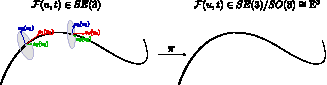
\includegraphics[width=0.9\textwidth]{figs_part2/sec7.5_kinematically_constrained_cosserat_rods/cosserat_rod_to_filament.pdf}
        \caption{(Left) A Cosserat rod, with configuration space $SE(3)$. (Right) A filament, with configuration space in $SE(3)/SO(3) \cong \mathbb{E}^3$.}
        \label{fig:cosserat rod and filament}
\end{figure}

Thus far we have considered the material frame $E$ and the center-line $\mathbf{r}$ as independent degrees of freedom, modelling a rod that can shear and twist in addition to bending and extending. In many applications it suffices to consider pure center-line dynamics where the cross-section does not shear \citep{eloyKinematicsMostEfficient2012, tornbergSimulatingDynamicsInteractions2004, goldsteinNonlinearDynamicsStiff1995, sodaDynamicsStiffChains1973, nordgrenComputationMotionElastic1974, hasimotoSolitonVortexFilament1972}. We shall refer to these systems as \textit{filaments}, and can be seen as a Cosserat rod model with a kinematically constrained material frame. As we will show, kinematic constraints can often be implemented by first identifying an appropriate Lie subgroup $H \subset SE(3)$ such that the homogeneous space $SE(3) / H$ is the kinematically constrained configuration space, and then by making a `gauge choice' $h(u) \in H$ which fixes a parametrisation of $SE(3) / H$. In addition to the filament, we will also consider the case of a \textit{twisting filament}, where the cross-section is allowed to twist around the center-line \citep{powersDynamicsFilamentsMembranes2010, parkerDerivationNonlinearRod1984a, goldsteinViscousNonlinearDynamics1998}.

\subsection{Kinematic constraints and gauge freedoms} \label{sec:Kinematic constraints and gauge freedoms}

The configuration space of a filament can be found by `rotating away' the material frame $E(u)$ at each $u$. Therefore the appropriate Lie subgroup is $H = SO(3)$, and the configuration space is $SE(3) / SO(3) \cong \mathbb{E}^3$, where $\mathbb{E}^3$ is the three-dimensional Euclidean space. Conceptually, that $SE(3)/SO(3)$ represents the configuration space of the filament can be understood by recalling the definition of a homogeneous space. For any Lie group $G$ and Lie subgroup $H \subset G$ then $G/H$ is the set
\begin{equation}
G / H = \{ gH\ |\ g \in G \}
\end{equation}
where $gH = \{ gh\ |\ h \in G \}$ is the left coset. Now consider the case when $G = SE(3)$ and $H = SO(3)$. Let $g_1 = (\mathbf{r}, E_1)$ and $g_2 = (\mathbf{r}, E_2)$ denote two cross-sections that are located at the same point $\mathbf{r}$, but have two different material frames $E_1$ and $E_2$, and furthermore we can trivially identify these as elements $g_1, g_2 \in SE(3)$. As $E_1$ is related to $E_2$ by a rotation in $SO(3)$, we have that $g_1 H = g_2 H$. In other words, in the homogeneous space $SE(3)/SO(3)$, $g_1$ and $g_2$ belong to the same element $g_1 H = g_2 H \in SE(3)/SO(3)$. Therefore, a filament can mathematically be described as a Cosserat rod where we have, for each $u$, identified all material frames $E(u)$ at $\mathbf{r}(u)$ as belonging to the same equivalence~class. See Fig.~\ref{fig:cosserat rod and filament} for an illustration.

Now let $\Phi : W \to SE(3)/SO(3)$ be the spatio-temporal configuration of the filament. As discussed in Sec.~\ref{sec:Sub-manifolds of homogeneous spaces}, we can write $\Phi$ as
\begin{equation} \label{eq:phi and phi tilde}
\Phi = \pi \circ \tilde{\Phi}
\end{equation}
where $\circ$ denotes compositions of maps and $\pi : SE(3) \to SE(3)/SO(3)$ relates elements in $SE(3)$ to elements in the homogeneous space and can be defined as
\begin{equation}
\pi( (\mathbf{r} ; E) ) = \mathbf{r},
\end{equation}
and $\tilde{\Phi} : W \to SE(3)$ is a \textit{framing}, or an \textit{adapted frame field}, of $\Phi$ \citep{clellandFrenetCartanMethod2017}, and is a Lie group-valued function on $W$ that satisfies Eq.~\ref{eq:phi and phi tilde}.

We can map any framing $\tilde{\Phi}$ to a spatio-temporal filament configuration $\Phi$ using Eq.~\ref{eq:phi and phi tilde}. Note however that this map is not injective. Let $h : W \to SO(3)$ be an arbitrary $SO(3)$-valued smooth function and let $\tilde{\Phi}_1 : W \to SE(3)$ and $\tilde{\Phi}_2 : W \to SE(3)$, then if $\tilde{\Phi}_1(t,u) = h(t,u) \tilde{\Phi}_2(t,u)$ maps to the same $\Phi$. Any given choice of $\tilde{\Phi}$ is called a \textit{framing} of $\Phi$ \citep{clellandFrenetCartanMethod2017}. There is thus a \textit{gauge freedom} in the choice of $\tilde{\Phi}$.

In principle, the kinodynamical equations for a Cosserat rod Eq.~\ref{eq:all eoms} apply to the filament as well. We could initialise Eq.~\ref{eq:all eoms} with some $\tilde{\Phi}(u, 0)$ that maps to the true initial condition $\Phi(u, 0)$, then simulate the equations of motion to find $\tilde{\Phi}(t,u)$, and then finally use Eq.~\ref{eq:phi and phi tilde} to find $\Phi(t, u)$. In this case, it is important that all constitutive and body forces and moments only couple to the center-line $\mathbf{r}$, and not the material frame $E$. For example, for conservative constitutive dynamics we could have a potential energy density $\mathcal{U} \propto \kappa^2$, where $\kappa$ is the scalar curvature of the center-line defined in Eq.~\ref{eq:scalar curvature}.

However, the above would mean simulating equations of motion of higher-dimensionality than the system in question, where the extra degrees of freedom (the material frame) are non-physical. In the following we will instead choose a particular \textit{gauge} and form an injective map between $\tilde{\Phi}$ and $\Phi$. In other words, by choosing a gauge we choose a particular prescription for how to frame a given space-curve. Beyond the fact that the resulting dynamics will be defined directly on the lower dimensional $SE(3)/SO(3)$ rather than $SE(3)$, it is also often easier to formulate constitutive dynamics given a particular framing, rather than formulating it in terms of the degrees of freedom of a general Cosserat rod. The programmatic construction of such gauges is better known as the \textit{theory of moving frames} \citep{cartanTheorieGroupesFinis1938, levyReviewElieCartan1935}. We note that the terminological use of `gauge', although well-motivated in this context, is not standard in the theory of moving frames.

All gauge choices are ultimately mathematically equivalent, however some choices are more practically useful than others. Our procedure to construct a gauge will be to write the material frame $E = (\mathbf{e}_1\ \mathbf{e}_2\ \mathbf{e}_3)$ as a function of the center-line $\mathbf{r}$. Thus one-to-one map between $\Phi$ and $\tilde{\Phi}$ is formed. As a first step towards finding an appropriate gauge, we set
\begin{equation} \label{eq:e1 tangent to r}
\mathbf{e}_1 = \frac{\mathbf{r}'}{h}
\end{equation}
where $h = |\mathbf{r}'|$, such that $\mathbf{e}_1$ is a unit-vector tangent to $\mathbf{r}$ at $u$. This means that given $\mathbf{e}_1$ we can write the center-line as
\begin{equation} \label{eq:r from e1}
\mathbf{r}(t, u) = \mathbf{r}(0, t) + \int_0^u h \mathbf{e}_1 du.
\end{equation} 
There is now a remaining $SO(2)$ gauge freedom in specifying the material frame vectors $\mathbf{e}_2$ and $\mathbf{e}_3$. In the gauges found in the literature \citep{bishopThereMoreOne1975a, mansfieldUseRotationMinimizing2019, clellandFrenetCartanMethod2017, carrollImprovingFrenetFrame2013, seligCharacterisationFrenetSerret2013}, most abide Eq.~\ref{eq:e1 tangent to r}, and are thus all related by an $SO(2)$ gauge transformation of $\mathbf{e}_2$ and $\mathbf{e}_3$.

\subsubsection*{The Frenet-Serret gauge}

In the \textit{Frenet-Serret} gauge \citep{frenetCourbesDoubleCourbure1852, serretQuelquesFormulesRelatives1851}, we set
\begin{equation} \label{eq:e2 in frenet-serret}
\mathbf{e}_2 = \frac{\mathbf{e}_1'}{\kappa}
\end{equation}
where $\kappa = |\mathbf{e}_1'|$ is the scalar curvature, such that $\mathbf{e}_2(u)$ is a unit-vector pointing in the direction of the center-line $\mathbf{r}(t,u)$ curves towards at time $t$. Eq.~\ref{eq:e2 in frenet-serret} fully specifies the frame, as $\mathbf{e}_3 = \mathbf{e}_1 \times \mathbf{e}_2$. In this context $\mathbf{e}_1$, $\mathbf{e}_2$ and $\mathbf{e}_3$ are called the tangent, normal and binormal vectors respectively. co

Now recall the equations of motion of $\mathbf{r}$ and $\mathbf{e}_i$ along $u$, given by Eq.~\ref{eq:dr and de}, which we write as
\begin{subequations}
\begin{align}
\mathbf{r}' & = \mathbf{e}_i \theta_i \\
\mathbf{e}_j' & = \mathbf{e}_i \hat{\pi}_{ij}.
\end{align}
\end{subequations}
Since $\mathbf{r}' = h \mathbf{e}_1$ we have that
\begin{equation} \label{eq:theta for filament}
\vec{\theta} = (h\ 0\ 0)^T,
\end{equation}
and as $\mathbf{e}_1' = \kappa \mathbf{e}_2$ we have that $\hat{\pi}_{21} = - \hat{\pi}_{12} = \kappa$ and $\hat{\pi}_{31} = -\hat{\pi}_{13} = 0$. This leaves only one more possible parameter $\hat{\pi}_{23} = -\hat{\pi}_{32}$, to which we assign the scalar parameter $\tau$, known as the \textit{torsion}. We thus have
\begin{equation} \label{eq:pi for filament}
\hat{\pi} = \begin{pmatrix}
0 & - \kappa & 0 \\
\kappa & 0 & - \tau \\
0 & \tau & 0.
\end{pmatrix}
\end{equation}
or, in vector form, $\vec{\pi} = (\tau\ 0\ \kappa)^T$. Finally, we get the \textit{Frenet-Serret equations}
\begin{equation} \label{eq:frennet-serret equations}
\begin{matrix}
\mathbf{e}_1' & = & & \kappa \mathbf{e}_2 & \\
\mathbf{e}_2' & = & - \kappa \mathbf{e}_1 & + & \tau \mathbf{e}_3 & \\
\mathbf{e}_3' & = &  & \tau \mathbf{e}2  &
\end{matrix}
\end{equation}
which together with Eq.~\ref{eq:r from e1} reconstructs the framing $\tilde{\Phi} \cong (\mathbf{r}, E)$, from which get the filament configuration $\Phi \cong \mathbf{r}$.

We see that by choosing a gauge, we have effectively constrained the spatial configuration $X$ to only take values in a subset $V \subset \mathfrak{se}(3)$, where $X = X(h, \kappa, \tau)$ is now parametrised by the three scalars $(h, \kappa, \tau)$ that are functions of space and time. Note that $V$ is not a Lie subalgebra. This constraint establishes an injective mapping between $V$-valued fields $X : W \to V$ and $\mathbb{E}^3$-valued fields $\Phi : W \to \mathbb{E}^3$. In this context $(h, \kappa, \tau)$ are known as the \textit{differential invariants} of the filament, as they uniquely define the filament up to rigid body transformations.

We should stress that in the mathematical literature, the purview of the theory of moving frames are in general space curves (rather than space-time curves). Furthermore, in that context the metric $h$ along the center-line is of little importance (and is usually not referred to as a differential invariant), and thus the arc-length parameterisation is preferred. Eq.~\ref{eq:frennet-serret equations} is therefore more commonly written in terms of arc-length derivatives
\begin{equation} \label{eq:frennet-serret equations arc-length}
\begin{matrix}
\partial_s \mathbf{e}_1 & = & & \tilde{\kappa} \mathbf{e}_2 & \\
\partial_s \mathbf{e}_2 & = & - \tilde{\kappa} \mathbf{e}_1 & + & \tilde{\tau} \mathbf{e}_3 & \\
\partial_s \mathbf{e}_3 & = &  & \tilde{\tau} \mathbf{e}2  &
\end{matrix}
\end{equation}
where $\tilde{\kappa} = h \kappa$ and $\tilde{\tau} = h \tau$ are the scalar curvature and torsion in the arc-length parameterisation.

Intuitively, we can visualise the motion of $(\mathbf{r}, E)$ as a function of $u$, for fixed $t$, in the Frenet-Serret gauge as follows. We can imagine an airplane which is travelling in the direction of $\mathbf{e}_1$ and with the floor of the plane aligned with $\mathbf{e}_3$. Its trajectory traces out a center-line $\mathbf{r}(u)$, at `speed' $h$. The Frenet-Serret frame corresponds to a plane that navigates \textit{pitching} (at a rate $\kappa$) and \textit{rolling} (at a rate $\tau$), but never \textit{yaws}.

We now consider the kinematics along time $t$. The same kinematic equations of motion Eq.~\ref{eq:kinematic equations of motion in the moving frame} for the Cosserat rod still apply. However, substituting $\vec{\theta} = (h\ 0\ 0)^T$ and $\vec{\pi} = (\tau\ 0\ \kappa)^T$ into Eq.~\ref{eq:kinematic equations of motion in the moving frame} we find the following constraints
\begin{subequations} \label{eq:angular velocity in frenet-serret}
\begin{align}
\Omega_1 & = (\Omega_3 \tau - \Omega_2') / \kappa \\
\Omega_2 & = - h^{-1} (D_u \vec{V})_3 \\
\Omega_3 & = h^{-1} (D_u \vec{V})_2.
\end{align}
\end{subequations}
It is intuitive that the angular velocity of the filament, with a cross-section constrained to be aligned with the center-line, is completely determined as a function of the differential invariants and the translational velocity $\vec{V}$. Eq.~\ref{eq:angular velocity in frenet-serret}, together with Eq.~\ref{eq:kinematic equations of motion in the moving frame}, completely specify the kinematics of the filament. Just as we have three scalar parameters $(h, \kappa, \tau)$ that determine the spatial configuration of the filament, the temporal evolution is determined by the three scalars in $\vec{V} = (V_1\ V_2\ V_3)$. Using Eq.~\ref{eq:kinematic equations of motion in the moving frame} and Eq.~\ref{eq:angular velocity in frenet-serret}, we can write the kinematic equations of motion for the filament compactly as
\begin{subequations} \label{eq:filament kinematic equtions of motion}
\begin{align}
\dot{h} & = V_1' - \kappa V_2 \\
\dot{\kappa} & = \Omega_3' + \tau \Omega_2 \\
\dot{\tau} & = \Omega_1' - \kappa \Omega_2 \\
\end{align}
\end{subequations}
where $\vec{\Omega}$ is given by Eq.~\ref{eq:angular velocity in frenet-serret}. The temporal evolution of the filament is thus specified by the velocity field $\vec{V}$ alone.

%\subsubsection{The Bishop gauge}

%The \textit{Bishop} gauge \citep{bishopThereMoreOne1975a, carrollImprovingFrenetFrame2013} is an alternative to the Frenet-Serret frame.

\subsubsection*{The twisting filament}

We can model a filament that can twist around its center-line by keeping the $SO(2)$ gauge freedom of $(\mathbf{e}_2, \mathbf{e}_3)$ and promoting it to a kinematic degree of freedom. The resulting degrees of freedom are then $\vec{\theta} = (h\ 0\ 0)^T$ as before and $\vec{\pi}$ has all three of its components. The resulting constraints on $\vec{\Omega}$ are then
\begin{subequations} \label{eq:angular velocity for twisting filament}
\begin{align}
\Omega_2 & = - h^{-1} (D_u \vec{V})_3 \\
\Omega_3 & = h^{-1} (D_u \vec{V})_2.
\end{align}
\end{subequations}
instead of Eq.~\ref{eq:angular velocity in frenet-serret}. The resulting kinematic equations of motion are thus
\begin{subequations} \label{eq:twisting filament kinematic equtions of motion}
\begin{align}
\dot{h} & = V_1' - \kappa V_2 \\
\dot{\vec{\pi}} & = D_u \vec{\Omega}
\end{align}
\end{subequations}
The temporal evolution of the twisting filament is thus specified by the rate of twist $\Omega_1$ and the velocity field $\vec{V}$.

In our airplane analogy, the twisting filament travels (again, as a function of $u$ for fixed $t$) by rolling (at a rate $\pi_1$), yawing (at a rate $\pi_2$) and pitches (at a rate $\pi_3$).

\subsection{Kinematically constrained dynamics} \label{sec:Kinematically constrained dynamics (cosserat rod)}

The formulation of the dynamics for kinematically constrained rods carries through less programmatically than in the case of the Cosserat rod. In general, extra care must be taken formulating the dynamics when the configuration space is a homogeneous space $G / H$. Issues of under- or over-determination in the equations of motion may arise due to the fact that $\text{dim}(G/H) < \text{dim}(G)$ if $\text{dim}(H) \neq 0$.

\subsubsection*{Filament dynamics}

For a filament, though its configuration space is $SE(3)/SO(3) \cong \mathbb{E}^3$ rather than $SE(3)$ as for the Cosserat rod, $SE(3)$ acts \textit{transitively} on $\mathbb{E}^3$. By which we mean that for any two elements $\mathbf{x}, \mathbf{y} \in \mathbb{E}^3$, there exists an element $g \in SE(3)$ such that $\mathbf{y} = g \mathbf{x}$. As before, we can define a Lagrangian density $\mathcal{L} : SE(3) \times TSE(3) \to \mathbb{R}$, with reduction $\ell : \mathfrak{se}(3) \to \mathbb{R}$, or use the Lagrange-D'Alembert principle as the starting point. The derivation of the dynamics then proceed as before in Sec.~\ref{sec:Cosserat rod dynamics}, and we find the same general equations of motion Eq.~\ref{eq:all eoms}.

However, issues arise as the dimension of the Lie algebra $\text{dim}(\mathfrak{se}(3)) = 6$ is larger than the configuration space $\text{dim}(\mathbb{E}^3) = 3$. This is in principle partially ameliorated by choosing a gauge, such as the Frenet-Serret gauge, but if this is done naively then the resulting equations of motion are untenable. Consider the dynamical equations of motion that would result if we consider a filament with the Frenet-Serret frame, starting from the Lagrange-D'Alembert principle Eq.~\ref{eq:lagrange-dalembert for non-monogenic constitutive forces and body forces}. As before, we let $S = \frac{\partial \mathcal{K}}{\partial N}$, where the reduced kinetic energy $\mathcal{K}$ of the Cosserat rod was derived in Eq.~\ref{eq:reduced kinetic energy} and we repeat it here
\begin{equation}
\mathcal{K}(N)  = \frac{1}{2} \rho_0 |\vec{V}|^2 +  \frac{1}{2} \vec{\Omega}^T \mathbb{I} \vec{\Omega}.
\end{equation}
Consider now, in particular, the moment balance equation for the filament
\begin{equation} \label{eq:moment balance filament wrong}
D_t \vec{L} = D_u \vec{M} + \vec{\theta} \times \vec{F} + \vec{m},
\end{equation}
where $\vec{L} = \mathbb{I} \vec{\Omega}$. Due to Eq.~\ref{eq:angular velocity in frenet-serret}, $\vec{\Omega}$ is not an independent degree of freedom, but a function of $\vec{V}$ and the differential invariants. Therefore Eq.~\ref{eq:moment balance filament wrong} over-determines the system, and is in general an intractable constraint.

To address this issue, we first note that it stems from the particular method by which we have parametrised the filament. In the fixed frame, the dynamics of the filament can be unambiguously written as
\begin{equation} \label{eq:fixed frame filament dynamics}
\rho_0 \ddot{\mathbf{r}} = \mathbf{F}' + \mathbf{f}
\end{equation}
where we used $\mathbf{P} = \rho_0 \dot{\mathbf{r}}$, which can be seen as the $1$-dimensional analogue of the Cauchy momentum equation in the Lagrangian point-of-view, where $\mathbf{F}$ would correspond to the \textit{first Piola-Kirchhoff stress tensor} in continuum dynamics.

In the geometric formulation presented here, we parametrise the filament in terms of its intrinsic geometry $\kappa$ and $\tau$, which corresponds to a given framing, rather than its center-line $\mathbf{r}(t,u)$ as in Eq.~\ref{eq:fixed frame filament dynamics}. This means that we must consider how the forces on the filament corresponds to moments on the moving frame $(\mathbf{e}_1, \mathbf{e}_2, \mathbf{e}_3)$. However, as the filament is ultimately described as a center-line, the model does not accommodate the angular momentum of its frame as an independent degree of freedom. In the literature the issue of Eq.~\ref{eq:moment balance filament wrong} is avoided by taking the overdamped limit modelling a filament immersed in a highly viscous fluid \citep{eloyKinematicsMostEfficient2012, tornbergSimulatingDynamicsInteractions2004, goldsteinNonlinearDynamicsStiff1995, sodaDynamicsStiffChains1973, nordgrenComputationMotionElastic1974, hasimotoSolitonVortexFilament1972, powersDynamicsFilamentsMembranes2010, goldsteinViscousNonlinearDynamics1998}, or by considering filament statics \citep{parkerDerivationNonlinearRod1984a}. Here, we avoid this limit and present a derivation of inertial filament dynamics.

Let $\mathcal{K}(N)  = \frac{1}{2} \rho_0 |\vec{V}|^2$, so that we get $S = \{ \vec{P} ; \vec{0} \}$ where $\vec{P} = \rho_0 \vec{V}$, therefore implicitly assuming the angular momentum of the filament to be negligible. The moment balance equation then becomes
\begin{equation} \label{eq:moment balance filament}
0 = D_u \vec{M} + \vec{\theta} \times \vec{F} + \vec{m}.
\end{equation}
To find self-consistent constitutive dynamics, we consider moment balance in the absence of external moments $\vec{m} = 0$, to find
\begin{subequations} \label{eq:filament force constraints}
\begin{align}
0 &  = (D_u \vec{M})_1 \\
F_2 & = h^{-1} (D_u \vec{M})_3 \\
F_3 & = - h^{-1} (D_u \vec{M})_2.
\end{align}
\end{subequations}
Thus we see that combined we can only independently specify three of the six force and moment components in total. The kinodynamical equations of motion for the filament are thus
\begin{subequations} \label{eq:filament dynamic equtions of motion}
\begin{align}
\dot{h} & = V_1' - \kappa V_2 \\
\dot{\kappa} & = \Omega_3' + \tau \Omega_2 \\
\dot{\tau} & = \Omega_1' - \kappa \Omega_2 \\
D_t \vec{P} & = D_u \vec{F} + \vec{f},
\end{align}
\end{subequations}
where the material derivatives are computed as before, using $\vec{\pi} = (\tau\ 0\ \kappa)$ and $\vec{\Omega}$ given by Eq.~\ref{eq:angular velocity in frenet-serret}, and where the force must obey the conditions Eq.~\ref{eq:filament force constraints}. We note that $\vec{M}$ does not appear explicitly in the dynamics, and we can indeed in theory write down the three arbitrary constitutive force components $\vec{F}$, which would induce a moment via Eq.~\ref{eq:filament force constraints} that has no impact on the dynamics. This is however not how the constitutive forces and moments are defined in practice, as we will now show.

We now move on to treat conservative constitutive dynamics. As discussed in \citep{levyReviewElieCartan1935}, when the Lie algebra, that acts transitively on the configuration space, is of a higher dimension than the configuration space the resulting Lagrangian dynamics (i.e. conservative dynamics) is under-determined. For a Cosserat rod we have $Q = \frac{\partial \mathcal{U}}{\partial X} = \{ \vec{F} ; \vec{M} \}^*$ which results in Eq.~\ref{eq:F_i and M_i from U}. In contrast, as $\vec{\theta} = (h\ 0\ 0)^T$ and $\vec{\pi} = (\tau\ 0\ \kappa)^T$ for a filament, the only components that are determined for a general constitutive $\mathcal{U}$ are
\begin{subequations} \label{eq:F1, M2 and M3 for filament}
\begin{align}
F_1 & =  \frac{\partial \mathcal{U}}{\partial h} \\
M_1 & =  \frac{\partial \mathcal{U}}{\partial \tau} \\
M_3 & =  \frac{\partial \mathcal{U}}{\partial \kappa} 
\end{align}
\end{subequations}
leaving $M_2$, $F_2$ and $F_3$ undetermined by $\mathcal{U}$. However we see that by having chosen a gauge, these force and moment components are given by moment balance Eq.~\ref{eq:filament force constraints}. The conservative constitutive forces and moments on a filament are thus determined by Eq.~\ref{eq:F1, M2 and M3 for filament} and Eq.~\ref{eq:filament force constraints} together. Note that it was necessary to let $M_1$, $F_2$ and $F_3$ be undetermined by $\mathcal{U}$, rather than setting $M_1 = F_2 = F_3 = 0$, which would conflict with moment balance. The above is consistent with the force and moment balance equations found for the filament in the overdamped setting \citep{powersDynamicsFilamentsMembranes2010} and in statics \citep{parkerDerivationNonlinearRod1984a}.

It is standard for filament dynamics to associate an energetic cost to the square of the curvature and extension $\mathcal{U} = \frac{1}{2} \epsilon \kappa^2$.  From Eq.~\ref{eq:F1, M2 and M3 for filament} and Eq.~\ref{eq:filament force constraints} we then find, expressed in a non-moving frame
\begin{equation} \label{eq:bernoulli moment for filament}
\mathbf{M} = \epsilon \kappa \mathbf{e}_3
\end{equation}
where $\epsilon$ is the bending stiffness. Eq.~\ref{eq:bernoulli moment for filament} agree with classical Bernoulli-Euler beam theory \citep{ powersDynamicsFilamentsMembranes2010, sodaDynamicsStiffChains1973, nordgrenComputationMotionElastic1974}. Note that as the notion of torsion $\tau$ appears from the gauge choice, rather than representing a physical property of the filament, a $\tau^2$ term is usually not included in $\mathcal{U}$. Therefore $M_1 = M_2 = 0$ for a filament in the Frenet-Serret frame in practice.

In the overdamped limit, the results of Sec.~\ref{sec:Dissipative and overdamped dynamics} and Eq.~\ref{eq:overdamped equations of motion in moving frame} applies as before, under the constraints Eq.~\ref{eq:theta for filament} and Eq.~\ref{eq:pi for filament}, Eq.~\ref{eq:angular velocity in frenet-serret} and Eq.~\ref{eq:filament force constraints}. Setting $\vec{f} = - \gamma_T \vec{V}$ we get
\begin{subequations} \label{eq:filament overdamped equtions of motion}
\begin{align}
\dot{h} & = V_1' - \kappa V_2 \\
\dot{\kappa} & = \Omega_3' + \tau \Omega_2 \\
\dot{\tau} & = \Omega_1' - \kappa \Omega_2 \\
\vec{V} & = \mu_T D_u \vec{F},
\end{align}
\end{subequations}
where $\mu_T = \gamma_T^{-1}$.

\subsubsection*{Twisting filament dynamics}

For a twisting filament, the angular velocity component $\Omega_1$ is now a dynamic degree of freedom, and we therefore permit angular momentum along the tangential direction. We assume the principal axes of the moment of inertia $\mathbb{I}$ coincide with the moving frame $\mathbf{e}_i,\ i=1,2,3$, and that the angular momentum is negligible along the normal and binormal directions, setting $\vec{L} = ( \mathbb{I}^{(1)} \Omega_1\ 0\ 0 )^T$, where $\mathbb{I}^{(1)}$ is the eigenvalue of $\mathbb{I}$ along $\mathbf{e}_1$. The resulting kinodynamical equations of motion are
\begin{subequations} \label{eq:twisting filament dynamic equtions of motion}
\begin{align}
\dot{h} & = V_1' - \kappa V_2 \\
\dot{\pi} & = D_u \vec{\Omega} \\
D_t \vec{P} & = D_u \vec{F} + \vec{f} \\
\mathbb{I}^{(1)} \dot{\Omega}_1 & = (D_u \vec{M})_1 + m_1
\end{align}
\end{subequations}
where the constraints on the force are
\begin{subequations} \label{eq:twisting filament force constraints}
\begin{align}
F_2 & = h^{-1} (D_u \vec{M})_3 \\
F_3 & = - h^{-1} (D_u \vec{M})_2,
\end{align}
\end{subequations}
which should be compared with Eq.~\ref{eq:filament dynamic equtions of motion} and Eq.~\ref{eq:filament force constraints}. For conservative constitutive we now have the relations
\begin{subequations} \label{eq:F1 and M for twisting filament}
\begin{align}
F_1 & =  \frac{\partial \mathcal{U}}{\partial h} \\
M_i & =  \frac{\partial \mathcal{U}}{\partial \pi_i}.
\end{align}
\end{subequations}


\begin{comment}
\subsubsection*{Inextensible Cosserat rods and filaments}

A Cosserat rod is \textit{inextensible} if it satisfies the kinematic constraint $\dot{h} = 0$. 


We will now consider the case of an inextensible Cosserat rod in the
overdamped limit, under the influence of a constitutive force $\vec{F}$.
For an inextensible rod, the tangential component of the force, tangent
to the center-line $\mathbf{r}$, is a constraining tension that enforces $\mathbf{r}'\cdot\mathbf{r}'=\boldsymbol{\theta}\cdot\boldsymbol{\theta}=1$.
Using Eq. \ref{eq:theta eom} and Eq. \ref{eq:V overdamped} we find
that the force must satisfy

\begin{equation}
\vec{\theta}^{T}D_{u}^{2}\vec{F}=0.\label{eq:Ft constraint}
\end{equation}
Equation \ref{eq:Ft constraint} should be seen as a constraint on
$F_{1}$. Though in practice it is often more covenient to consider
a tension force $\vec{T}$ separate from the rest of the constitutive
dynamics $\vec{F}$, such that the total force on the filament be
$\tilde{\vec{F}}=\vec{F}+\vec{T}$. As a tensional force must act
tangentially along the filament, we must have $\vec{T}\propto\vec{\theta}$,
and so we write $\vec{T}=T\vec{\theta}$. The tension force will enforce
the condition $\partial_{t}(\vec{\theta}^{T}\vec{\theta})=2\dot{\vec{\theta}}^{T}\vec{\theta}=0$.
From Eq. \ref{eq:Ft constraint} we find
\begin{equation}
\vec{\theta}^{T}\partial_{u}^{2}(\vec{F}+T\vec{\theta})=0\label{eq:tension}
\end{equation}
which is a non-linear 2nd order ODE for $T$. Note that using Eq.
\ref{eq:tension} renders the component of the force tangent to the
center-line $F_{\theta}=\boldsymbol{\theta}\cdot\mathbf{F}$ redundant
and has no effect on the system. Using $\theta_{i}\theta_{i}=1$ and
$\partial_{u}(\theta_{i}\theta_{i})=2\theta_{i}'\theta_{i}=0$, Eq.
\ref{eq:tension} simplifes to
\begin{equation}
(\partial_{u}^{2}-H)T=-\vec{\theta}^{T}D_{u}^{2}\vec{F}\label{eq:tension eq}
\end{equation}
where $H=-\theta_{i}\theta_{i}''+2\theta_{i}\hat{\pi}_{ij}\theta_{j}'-\theta_{i}\hat{\pi}_{ij}\hat{\pi}_{jk}\theta_{k}$.
In numerical experiments Eq. \ref{eq:tension} would have to be solved
at each time-step to compute the tensional force.

For a special Cosserat rod or filament the constraint simplifies to
$\theta_{1}=h=1$, implying $\dot{h}=0$. Furthermore, $F_{1}=F_{\theta}$
is now tangent to the center-line. The equation for $T$ simplifies
to
\begin{equation}
(\partial_{s}^{2}-(\pi_{2}^{2}+\pi_{3}^{2}))T=-\nabla_{u}^{2}F_{1}
\end{equation}
and $\mathbf{T}=T\mathbf{e}_{1}$. Note that the tangential component
of the force $F_{1}$ is redundant here, and can be safely set to
zero.
\end{comment}


\section{The hyperelastic Cosserat rod model} \label{sec:The hyperelastic Cosserat rod model}

In many applications the conservative part of the constitutive dynamics arise from a potential of the form Eq.~\ref{eq:U quadratic form} \citep{NonlinearProblemsElasticity2005, wangOptimalControlSoft2021a, gargSlenderBodyTheory2022, tillRealtimeDynamicsSoft2019}, where the potential $\mathcal{U}$ is a quadratic form in $X$, with coefficients given by the symmetric and positive-definite stiffness matrix $\mathsf{K} \in \mathbb{R}^{6 \times 6}$. Here we derive the form of $\mathsf{K}$ from first principles, given constitutive assumptions on the material that the rod is composed of. Specifically, we model the Cosserat rod as a slender tube of hyper-elastic \textit{Saint Venant-Kirchoff} material \cite{basarNonlinearContinuumMechanics2013}, but the derivation carries through regardless of what constitutive assumption.

We consider a straight rod $\mathscr{M}=\mathscr{D} \times [0,L_{0}]$ at rest, where $\mathscr{D}$ is a disc of arbitrary shape, and $L_{0}$ is the length of the rod.
As before, $\mathbf{X}$ is the material coordinate on $\mathscr{M}$, and we align $X_{1}\in[0,L_{0}]$ along the length of the rod, and $(X_{2},X_{3})\in\mathscr{D}$. We will use $u = X_1$ and $X_1$ interchangeably. Deformations of $\mathscr{M}$ are given by $\mathbf{x}(\mathbf{X})$, which we will refer to as the \textit{deformed coordinate}. The material and deformed coordinates can be related as
\begin{equation}
d\mathbf{x}= \mathcal{P} d\mathbf{X}
\end{equation}
where $\mathcal{P} =\frac{\partial\mathbf{x}}{\partial\mathbf{X}}$ is here the \emph{deformation
gradient tensor}, and we write its components in the moving frame $\mathcal{P}_{ij} = \mathbf{e}_i \cdot \left( \frac{\partial\mathbf{x}}{\partial\mathbf{X}} \mathbf{e}_j \right)$. Following \citep{landauTheoryElasticityVolume1986}, we consider
the change in infinitesimal distances between two material points $\mathbf{X}_{1}$ and $\mathbf{X}_{2}$ in the rod after a deformation. In the undeformed
state, the distance between $\mathbf{X}_{1}$ and $\mathbf{X}_{2}$
is $d\ell^{2}=|d\mathbf{X}|^{2}$. After deformation we have
\begin{equation} \label{eq:deformation}
\begin{aligned}d\ell'^{2}=|d\mathbf{x}|^{2} & =(Pd\mathbf{X})^{T}(\mathcal{P} d\mathbf{X})\\
 & =d\mathbf{X}^{T} \mathcal{P}^{T} \mathcal{P} d\mathbf{X}\\
 & =d\ell^{2}+2d\mathbf{X}^{T}Ed\mathbf{X}\\
 & =d\mathbf{X}^{T}(I+2E)d\mathbf{X}
\end{aligned}
\end{equation}
where
\begin{equation} \label{eq:Lagrangian strain tensor}
E=\frac{1}{2}\left(\frac{\partial\mathbf{u}}{\partial\mathbf{X}}+\left(\frac{\partial\mathbf{u}}{\partial\mathbf{X}}\right)^{T}+\left(\frac{\partial\mathbf{u}}{\partial\mathbf{X}}\right)^{T}\frac{\partial\mathbf{u}}{\partial\mathbf{X}}\right) 
\end{equation}
is the \emph{Lagrangian strain tensor} and $\mathbf{u}(\mathbf{X})=\mathbf{x}-\mathbf{X}$ is the \emph{deformation vector}. For small deformations, we can approximate
Eq. \ref{eq:deformation assumption} as $E\approx\frac{1}{2}\left(\frac{\partial\mathbf{u}}{\partial\mathbf{X}}+\left(\frac{\partial\mathbf{u}}{\partial\mathbf{X}}\right)^{T}\right)$,
in which case we can express it as
\begin{equation} \label{eq:approximated E}
E=\frac{1}{2}(\mathcal{P}+\mathcal{P}^{T}-2 \mathbbm{1}).
\end{equation}
The Lagrangian strain tensor can be seen as giving the relative deformations
along the principle axes of a material, where the latter are defined as the eigenvectors $E$. The elastic energy density of the material in a deformed state is a function of $E$, and we assume it to be a quadratic form
\begin{equation} \label{eq:general Kirchoff W}
W(E) = \frac{1}{2} C_{ijkl} E_{ij} E_{kl}
\end{equation}
where $C_{ijkl}$ is a fourth-order tensor of elastic constants, which is known as the Saint Venant-Kirchoff constitutive assumption \cite{basarNonlinearContinuumMechanics2013}, and materials that are well-approximated under this assumption are known as \textit{Saint Venant-Kirchoff materials}. If we assume that $C$ is isotropic, in which case it has the form
\begin{equation}
C_{ijkl} = \lambda \delta_{ij} \delta_{kl} + \mu_1 \delta_{ik} \delta_{jl} + \mu_2 \delta_{il} \delta_{jk}
\end{equation}
then Eq.~\ref{eq:general Kirchoff W} can be shown to reduce to
\begin{equation} \label{eq:elastic energy per volume}
W(E)=\mu\text{Tr}(E^{2})+\frac{\lambda}{2}\text{Tr}(E)^{2}
\end{equation}
where $\lambda$ and $\mu = \mu_1 + \mu_2$ are known as the \textit{Lamé constants}.

We will now proceed to derive the potential energy per unit material length of a Cosserat rod under the constitutive assumption of Eq.~\ref{eq:elastic energy per volume}. We impose the kinematic assumption Eq.~\ref{eq:cosserat rod kinematic assumption}, which we write again here as
\begin{equation}
\mathbf{x}(\mathbf{X})=\mathbf{r}(X_{1})+\mathbf{e}_{\xi}X_{\xi},\ \xi=2,3\label{eq:deformation assumption}
\end{equation}
which constrains deformations to preserve the area and shape of the cross-section at each $X_{1}$. Since
\begin{equation}
\frac{\partial \mathbf{x}}{\partial X_1} = \theta_i \mathbf{e}_i + \mathbf{e}_i \hat{\pi}_{i \gamma} X_\gamma, \quad \gamma = 2,3
\end{equation}
where we used Eq.~\ref{eq:dr and de}, we have
\begin{equation} \label{eq:P cosserat rod}
\begin{aligned}
\mathcal{P}_{i1} & =\theta_{i}+ \pi_{i \gamma} X_{\gamma}\\
\mathcal{P}_{i\gamma} & =\delta_{i\gamma}.
\end{aligned}
\end{equation}
The Lagrangian strain tensor $E$ can then be computed using Eq.~\ref{eq:approximated E}, and since Eq.~\ref{eq:P cosserat rod} is expressed entirely in terms of $X = \{ \vec{\theta} ; \vec{\pi} \}$, we can express the energy volume density $W$ as a function of $X$ as well. To find the energy density per unit-length $\mathcal{U}(\vec{\theta}, \vec{\pi})$ of the rod, we must integrate out the cross-section
\begin{equation}
\mathcal{U}(\vec{\theta}, \vec{\pi})=\int_{\mathscr{D}}W(E)dX_{2}dX_{3}.
\end{equation}
For simplicity, we assume a circular cross-section, for which we have that
\begin{equation} \label{eq:cross section integrals}
\begin{aligned}\int_{\mathscr{D}}dA & =\pi R^{2}\\
\int_{\mathscr{D}}X_{\alpha}dA & =0\\
\int_{\mathscr{D}}X_{\alpha}X_{\beta}dA & =\frac{\pi R^{4}}{4}\delta_{\alpha\beta}\\
\int_{\mathscr{D}}X_{\alpha}X_{\beta}X_{\gamma}dA & =0\\
\int_{\mathscr{D}}X_{\alpha}X_{\beta}X_{\gamma}X_{\delta}dA & =\begin{cases}
\frac{\pi R^{6}}{8}, & \alpha=\beta=\gamma=\delta\\
\frac{\pi R^{6}}{24}, & \alpha=\beta\text{ and }\gamma=\delta\\
\frac{\pi R^{6}}{24}, & \alpha=\gamma\text{ and }\gamma=\beta
\end{cases}
\end{aligned}
{U}
\end{equation}
where $\alpha,\beta,\gamma,\delta=2,3$ and $R$ is the radius of
the rod. From Eq.~\ref{eq:cross section integrals}, Eq.~\ref{eq:cross section integrals}, Eq.~\ref{eq:approximated E} and Eq.~\ref{eq:elastic energy per volume}, the potential energy per unit material length evaluates to
\begin{equation} \label{eq:hyperelastic cosserat rod circular cross-section}
\mathcal{U}(\vec{\theta}, \vec{\pi})=\frac{k_{1}}{2}(\theta_{1}-1)^{2}+\frac{k_2}{2}(\theta_{2}^{2}+\theta_{3}^{2})+\frac{\epsilon_1}{2}\hat{\pi}_{1}^{2}+\frac{\epsilon_2}{2}(\hat{\pi}_{2}^{2}+\hat{\pi}_{3}^{3})
\end{equation}
where $k_1=\pi R^{2}(\lambda+2\mu)$, $k_2=\frac{\pi R^{2}}{2}\lambda$, $\epsilon_1=\frac{\pi R^{4}}{4}\lambda$ and $\epsilon_2=\frac{\pi R^{4}}{4}(\lambda+2\mu)$. Equation \ref{eq:hyperelastic cosserat rod circular cross-section} is consistent with the is consistent with the quadratic Cosserat free energies found in the literature \citep{giusteriSimulationViscoelasticCosserat2021, caoNonlinearDynamicsElastic2008, rubinCosseratRods2000}. For a non-circular cross-section we will in general have a potential energy of the form
\begin{equation} \label{eq:general U for hyperelastic rod}
\mathcal{U}(\vec{\theta}, \vec{\pi})=\frac{k_1}{2}(\theta_{1}-1)^{2}+\frac{k_{2}}{2}\theta_{2}^{2}+\frac{k_{3}}{2}\theta_{3}^{2}+\frac{\epsilon_1}{2}\hat{\pi}_{1}^{2}+\frac{\epsilon_{2}}{2}\hat{\pi}_{2}^{2}+\frac{\epsilon_{3}}{2}\hat{\pi}_{2}^{2}.
\end{equation}
We can interpret the form of the potential energy by recalling how $\vec{\theta}$ and $\vec{\pi}$ encodes the various kinematic deformations of the Cosserat rod, described in Sec.~\ref{sec:deformation types}. The first three terms in Eq.~\ref{eq:general U for hyperelastic rod} penalises both shearing of the material frame, as well as extension of the center-line. The $\pi_1$ term penalises twisting of the material frame along $\mathbf{e}_1$, and $\pi_2$ and $\pi_3$ penalises the rotation of the material frame along $\mathbf{e}_2$ and $\mathbf{e}_3$ respectively.

The stiffness matrix of a hyper-elastic Cosserat rod can thus be written as
\begin{equation}
\mathsf{K} = \begin{pmatrix}
K^{(1)} & 0_{3 \times 3} \\
0_{3 \times 3} & K^{(2)}
\end{pmatrix}
\end{equation}
where $K^{(1)} = \text{diag} \left\{ k_1, k_2, k_3 \right\}$ and $K^{(2)} = \text{diag} \left\{ \epsilon_1, \epsilon_2, \epsilon_3 \right\}$, with rest state
\begin{subequations}
\begin{align}
\vec{\theta}_0 & = (1\ 0\ 0)^T \\
\vec{\pi}_0 & = (0\ 0\ 0)^T.
\end{align}
\end{subequations}
The resulting constitutive force and moments are
\begin{subequations}
\begin{align}
\vec{F} & = \frac{\partial \mathcal{U}}{\partial \vec{\theta}} = K^{(1)} (\vec{\theta} - \vec{\theta}_0) \\
\vec{M} & = \frac{\partial \mathcal{U}}{\partial \vec{\pi}} = K^{(2)} \vec{\pi}.
\end{align}
\end{subequations}
We see that in this constitutive model, the force $\vec{F}$ acts on the center-line such as to align with its material frame. In other words, if the material frame is shearing, then the center-line will bend such as to be tangent to $\mathbf{e}_1$. If the material frame is rotating along $u$, which corresponds to a non-zero $\vec{\pi}$, then the moment $\vec{M}$ acts so as to render it non-rotating.  We thus see that a shearing material frame \textit{induces} bend. This effect happens despite the fact that $\vec{\theta}$ and $\vec{\pi}$ do not couple in $\mathcal{U}$, which inherently due to the geometric non-linearities in the kinematics of the Cosserat rod. Conversely, a bending center-line which is aligned with the material frame will induce shear. Note that there is no direct energetic cost for the bending of the center-line itself (as $\mathcal{U}$ is not a function of the scalar curvature $\kappa$), however the energetic cost of shearing, combined with the energetic cost of a rotating material frame, conspire together so as to straighten segments of the rod that bend.

\section{Dissipative and overdamped dynamics} \label{sec:Dissipative and overdamped dynamics}

Equation \ref{eq:dynamics in terms of V and L with body forces} allows us to model general dissipative dynamics. We consider the case of a Cosserat rod that suffers both internal and external friction
\begin{subequations} 
\begin{align}
\dot{X} & = \mathcal{D}_u X \label{eq:kinematics with dissipation} \\
\mathcal{D}^*_t S & = \mathcal{D}^*_u Q - \mathsf{H} \dot{X} - \mathsf{G} N \label{eq:dynamics with dissipation} \\
Q & = 0, \quad u = 0, L_0, 
\end{align}
\end{subequations}
where we have set $T = - \mathsf{H} \dot{X} - \mathsf{G} N$, and where $\mathsf{H}$ and $\mathsf{G}$ are positive-definite matrices of damping coefficients of the internal and external friction respectively. Note that $\mathsf{H} \dot{X}$ in Eq.~\ref{eq:dynamics with dissipation} is evaluated by substituting in Eq.~\ref{eq:kinematics with dissipation}. If let the frictional matrices be block-diagonal in the translational and angular components as
\begin{subequations} 
\begin{align}
\mathsf{H} & = \begin{pmatrix}
	\gamma^\text{in}_T & 0_{3 \times 3} \\
	0_{3 \times 3} & \gamma^\text{in}_R
\end{pmatrix} \\ 
\mathsf{G} & = \begin{pmatrix}
	\gamma_T & 0_{3 \times 3} \\
	0_{3 \times 3} & \gamma_R
\end{pmatrix}
\end{align}
\end{subequations}
where $\gamma^\text{in}_T$, $\gamma^\text{in}_R$, $\gamma_T$ and $\gamma_R$ are positive-definite $3 \times 3$-matrices, we can write the equations of motion as
\begin{subequations} \label{eq:underdamped cosserat rod}
\begin{align}
D_t \vec{\theta} & = D_u \vec{V} \\
\partial_t \vec{\pi} & = D_u \vec{\Omega} \\
D_t \vec{P} & = D_u \vec{F} - \gamma^\text{in}_T \dot{\vec{\theta}} - \gamma_T \vec{V} \\
D_t \vec{L} & = D_u \vec{M} + \vec{\theta} \times \vec{F}  - \gamma^\text{in}_R \dot{\vec{\pi}} - \gamma_R \vec{\Omega}
\end{align}
\end{subequations}
where again $\gamma^\text{in}_T \dot{\vec{\theta}}$ and $\gamma^\text{in}_T \dot{\vec{\pi}}$ can be evaluated using the kinematic equations of motion, and $\vec{F} = \vec{M} = 0,\ u= 0,L_0$.

We can consider a limit where the dissipative forces dominate over the inertial forces (which correspond to the left-hand side of Eq.~\ref{eq:dynamics with dissipation}). In this limit, we set $S \approx 0$, or equivalently $\vec{P} \approx 0$ and $\vec{L} = \mathbb{I} \vec{\Omega} \approx 0$. The resulting equations are \textit{overdamped} equations of motion
\begin{subequations}  
\begin{align}
\dot{X} & = \mathcal{D}_u N \label{eq:overdamped kinematics} \\
\mathsf{G} N & = \mathcal{D}^*_u Q + \mathsf{H} \dot{X} \label{eq:overdamped dynamics} \\
Q & = 0, \quad u = 0, L_0.
\end{align}
\end{subequations}
where we must solve for $N$ in Eq.~\ref{eq:overdamped dynamics} to compute Eq.~\ref{eq:overdamped kinematics}. In terms of the translational and angular velocities, the equations of motion are
\begin{subequations} \label{eq:overdamped equations of motion in moving frame}
\begin{align}
D_t \vec{\theta} & = D_u \vec{V} \\
\partial_t \vec{\pi} & = D_u \vec{\Omega} \\
\gamma_T \vec{V} & = D_u \vec{F} - \gamma^\text{in}_T \dot{\vec{\theta}}  \\
\gamma_R \vec{\Omega} & = D_u \vec{M} + \vec{\theta} \times \vec{F}  - \gamma^\text{in}_R \dot{\vec{\pi}}
\end{align}
\end{subequations}
where again we must solve for $\vec{V}$ and $\vec{\Omega}$ in the latter two equations and substitute them into the kinematic equations of motion. We note that the overdamped equations of motion are first-order in time $t$ and second-order in space $u$ (as opposed to first-order in the underdamped case). Furthermore, the only degree of freedom is here $X = \{ \vec{\theta} ; \vec{\Omega} \}$, and so the dynamics are $6$-dimensional as opposed to $12$-dimensional in the underdamped case.

The presence of the internal friction $\mathsf{H} \dot{X}$ significantly complicates the evaluation of the overdamped dynamics. Substituting Eq.~\ref{eq:overdamped kinematics} into Eq.~\ref{eq:overdamped dynamics} we get a self-consistency relation for $N$
\begin{equation}
\mathsf{G} N = \mathcal{D}^*_u Q + \mathsf{H} \mathcal{D}_u N
\end{equation}
and formally we can write $N$ as
\begin{equation}
N = \mathscr{A}^{-1} \mathcal{D}^*_u Q
\end{equation}
where $\mathscr{A} = \mathsf{G} - \mathsf{H} (\partial_u + \text{ad}_X)$. In simulations, which invariably employ some discretisation scheme, $\mathscr{A}$ becomes a matrix that can be inverted numerically. If, however, we neglect internal dissipation we have $N = \mathsf{G}^{-1} \left( \partial_u - \text{ad}_X^* \right) Q$, and we can write the equations of motion in a compact form as
\begin{equation} \label{eq:Cosserat rod overdamped dynamics}
\dot{X}  = \mathcal{D}_u \left[ \mathsf{G}^{-1} \mathcal{D}^*_u Q \right],
\end{equation}
or equivalently
\begin{subequations} 
\begin{align}
D_t \vec{\theta} & = D_u \left[ \mu_T D_u \vec{F} \right] \\
\partial_t \vec{\pi} & = D_u \left[ \mu_R  D_u \vec{M} \right] 
\end{align}
\end{subequations}
where $\mu_{T,R} = \gamma_{T,R}^{-1}$, which would be the overdamped equations of motion of a Cosserat rod immersed in a viscous medium. 

\subsection{Inextensible rods}

We will now consider the case of an inextensible Cosserat rod in the
overdamped limit, under the influence of a constitutive force $\vec{F}$.
For an inextensible rod, the tangential component of the force, tangent
to the center-line $\mathbf{r}$, is a tension that must satisfy $\mathbf{r}'\cdot\mathbf{r}'=\boldsymbol{\theta}\cdot\boldsymbol{\theta}=1$.
Using Eq. \ref{eq:theta eom} and Eq. \ref{eq:V overdamped} we find
that the force must satisfy

\begin{equation}
\vec{\theta}^{T}D_{u}^{2}\vec{F}=0.\label{eq:Ft constraint}
\end{equation}
Equation \ref{eq:Ft constraint} should be seen as a constraint on
$F_{1}$. Though in practice it is often more covenient to consider
a tension force $\vec{T}$ separate from the rest of the constitutive
dynamics $\vec{F}$, such that the total force on the filament be
$\tilde{\vec{F}}=\vec{F}+\vec{T}$. As a tensional force must act
tangentially along the filament, we must have $\vec{T}\propto\vec{\theta}$,
and so we write $\vec{T}=T\vec{\theta}$. The tension force will enforce
the condition $\partial_{t}(\vec{\theta}^{T}\vec{\theta})=2\dot{\vec{\theta}}^{T}\vec{\theta}=0$.
From Eq. \ref{eq:Ft constraint} we find
\begin{equation}
\vec{\theta}^{T}\partial_{u}^{2}(\vec{F}+T\vec{\theta})=0\label{eq:tension}
\end{equation}
which is a non-linear 2nd order ODE for $T$. Note that using Eq.
\ref{eq:tension} renders the component of the force tangent to the
center-line $F_{\theta}=\boldsymbol{\theta}\cdot\mathbf{F}$ redundant
and has no effect on the system. Using $\theta_{i}\theta_{i}=1$ and
$\partial_{u}(\theta_{i}\theta_{i})=2\theta_{i}'\theta_{i}=0$, Eq.
\ref{eq:tension} simplifes to
\begin{equation}
(\partial_{u}^{2}-H)T=-\vec{\theta}^{T}D_{u}^{2}\vec{F}\label{eq:tension eq}
\end{equation}
where $H=-\theta_{i}\theta_{i}''+2\theta_{i}\hat{\pi}_{ij}\theta_{j}'-\theta_{i}\hat{\pi}_{ij}\hat{\pi}_{jk}\theta_{k}$.
In numerical experiments Eq. \ref{eq:tension} would have to be solved
at each time-step to compute the tensional force.

For a special Cosserat rod or filament the constraint simplifies to
$\theta_{1}=h=1$, implying $\dot{h}=0$. Furthermore, $F_{1}=F_{\theta}$
is now tangent to the center-line. The equation for $T$ simplifies
to
\begin{equation}
(\partial_{s}^{2}-(\pi_{2}^{2}+\pi_{3}^{2}))T=-\nabla_{u}^{2}F_{1}
\end{equation}
and $\mathbf{T}=T\mathbf{e}_{1}$. Note that the tangential component
of the force $F_{1}$ is redundant here, and can be safely set to
zero.

%%%% Ideas and notes:
 
% - In general $\mathcal{F}_0$ can be dependet on time and space, which would be the way to have a non-straight reference rod.

% - It would be good to show that the dynamics of a filament with a certain potential $U(\kappa)$ has the same dynamics as a Cosserat rod with the same potential.


\chapter{Geometric continuum mechanics on Lie group- and homogeneous configuration spaces} \label{ch:Geometric continuum mechanics on homogeneous configuration spaces}

In Ch.~\ref{ch:Cosserat rods}, we derived the kinodynamical equations of motion of the Cosserat rod and filament, systems in one material dimension with configuration space $SE(3)$ and $SE(3)/SO(3)$ respectively. In the subsequent section we provide a generalisation of Ch.~\ref{ch:Cosserat rods} to systems with general material bases spaces and homogeneous configuration spaces. We call this the \textit{geometrisation programme}. Mathematically, the geometrisation programme can be seen as a general field theory of Lie group- or homogeneous space-valued fields defined over topological manifolds. The derivations of the results are provided in Sec.~\ref{sec:Geometric kinematics} and Sec.~\ref{sec:Geometric dynamics}. 

We have separated the exposition of the results and their derivation, as the latter require a level of mathematical abstraction not necessary in the presentation of the geometrisation programme itself. The primary mathematical challenge stems from allowing arbitrary topologies in the material base space, which entails that it longer admits a global set of coordinates. An example of such a system would be a closed surface, like the membrane of a cell. This necessitated further geometrical abstraction that was not required in the case of the Cosserat rod. 

In Sec.~\ref{sec:geometrisation applications} we use the geometrisation programme to derive the equations of motion for a set of example systems. This section is called `\text{Applications}', meant to be understood in the sense that our general geometric framework is \emph{applied} to derive the kinodynamic theories of the given example systems. When these systems are well-established in the literature, we show that our framework recovers the correct equations of motion. Finally, in Sec.~\ref{sec:geometrisation discussion} we conclude with a summary and discussion on the geometrisation programme.

\section{The geometrisation programme} \label{sec:The geometrisation programme}

\begin{figure}[t]
\centering
        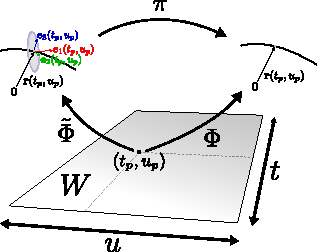
\includegraphics[width=0.8\textwidth]{figs_part2/ch8_geometrisation/cosserat_geometrisation.pdf}
        \caption{The relation between the spatio-temporal configuration $\Phi$ and the adapted frame field $\tilde{\Phi}$ of a filament, where the latter can be seen as the spatio-temporal configuration of a Cosserat rod. In the top-left and top-right we show the mapping of $(t_p, u_p)$, a point in the kinematic base space $W$, to $\tilde{\Phi}(t_p, u_p)$ and $\Phi(t_p, u_p)$, which are related by the projection map $\pi$.}\label{fig:cosserat rod geometrisation illustration}
\end{figure}

Here we generalise the results of Sec.~\ref{sec:Geometric Cosserat rod mechanics} to systems with an arbitrary material base space and homogeneous configuration space. To aid understanding it will be helpful to reintroduce some nomenclature, and to relate and contextualise the mathematical formulation of the Cosserat rod and the filament to the general systems that we describe in what follows. This preamble will thus serve as a brief overview of the results given in the subsequent subsections.

The \textit{material base space} of an open Cosserat rod is the manifold $M = [0, L_0]$, and its \textit{kinematic configuration space} is the Lie group $SE(3)$. The \textit{spatio-temporal configuration} of the Cosserat rod is a map $\Phi : W \to SE(3)$, where $W = [0,T] \times M$ is the \textit{kinematic base space} and $[0,T]$ the time domain. In Sec.~\ref{sec:Mechanics of kinematically constrained Cosserat rods} we showed that a filament can be considered a kinematically constrained Cosserat rod, and its configuration space is the homogeneous space $SE(3)/SO(3)$. The spatio-temporal configuration of the filament is thus $\Phi : W \to SE(3) / SO(3)$. However, the kinematics on the homogeneous space $SE(3) / SO(3)$ can be related to kinematics on the Lie group $SE(3)$ using an \textit{adapted frame field} (or \textit{framing}) $\tilde{\Phi} : W \to SE(3)$ via the composition $\Phi = \pi \circ \tilde{\Phi}$, where $\pi : SE(3) \to SO(3)$ is the projection map and is defined as $\pi((\mathbf{r} ; E)) = \mathbf{r}$. A given Cosserat rod configuration was thus seen as an adapted frame of the filament. This relationship is illustrated in Fig.~\ref{fig:cosserat rod geometrisation illustration}.

The mathematical formulation of the $SE(3)$-configured Cosserat rod, and its relation to the $SE(3)/SO(3)$-configured filament, is analogous to the more general setting we will develop here. We first consider kinematic configuration spaces that is a general Lie group $G$, and we will denote $\mathfrak{g}$ as its Lie algebra. Secondly, we let the material base space $M$ be a general manifold. Thirdly, given a Lie subgroup $H \subset G$ known as the \textit{stabiliser}, we can relate the kinodynamics of the $G$-configured system to a corresponding $G/H$-configured system by choosing a \textit{gauge} in $H$. Therefore, as in Ch.~\ref{ch:Cosserat rods}, it suffices to at first consider the kinodynamics of the $G$-configured system with material base space $M$. The corresponding $G/H$-configured system can then be modelled by applying kinematic constraints on the $G$-configured system.

The spatio-temporal configurations of the general systems in consideration are therefore $\Phi : M \to G$, or $\Phi : M \to G/H$. We can thus see the geometrisation programme as a general theory of $G$- or $G/H$-valued fields on topological manifolds $M$. The majority of the mathematical technology we introduce is then for the purpose of formulating the field equations of motion on the Lie algebra $\mathfrak{g}$, which locally acts transitively on $G/H$ (and on $G$, trivially).

In Sec.~\ref{sec:(summary) kinematics} and Sec.~\ref{sec:(summary) dynamics} we present the kinodynamic equations of motion of a general $G$-configured system with material base space $M$, formulated in terms of Lie algebraic quantities. In Sec.~\ref{sec:Adapted frames and gauge choices} we describe the procedure by which $G/H$-configured systems can be modelled via kinematically constraining the $G$-configured system. We conclude with a discussion of the geometrisation programme in Sec.~\ref{sec:geometrisation discussion}.

% In the above we have taken great care to consider a general $G/H$-configured system. However, as we saw in Sec.~\ref{sec:Mechanics of kinematically constrained Cosserat rods}, the equations of motion of a filament (which has a homogeneous configuration space) were expressed \emph{in terms} of those of the Cosserat rod (which has a Lie group configuration space). The same equations of motion Eq.~\ref{eq:all eoms} apply to both systems, but for the filament we had prescribed a particular \textit{gauge}, which amounted to a constraint on its degrees of freedom, forces and moments. In other words the kinodynamics of the $SE(3)/SO(3)$-configured filament was formulated in terms of the kinodynamics of $SO(3)$-configured Cosserat rod. 

% Generalising the previous statement, we have that the kinodynamics of a $G/H$-configured system can be modelled as constrained kinodynamics of the corresponding $G$-configured system. Completely analogously to Sec.~\ref{sec:Mechanics of kinematically constrained Cosserat rods}, adapted kinodynamics of a $G/H$-configured system can then be found by choosing a gauge in $H$, and by eliminating the requisite amount of dynamical degrees of freedom. Therefore, in the following, we formulate the equations of motion of a general $G$-configured system. In Sec.~\ref{sec:Adapted frames and gauge choices} we discuss the procedure through which $G/H$-configured systems can be modelled via kinematic constraint.

\subsection{Kinematics} \label{sec:(summary) kinematics}

A physical system can be kinematically described using the geometrisation programme if it is possible to identify its kinematic configuration at a material point with an element of a Lie group $G$. Alternatively, the programme is also applicable if the kinematic configuration space can be identified with a homogeneous space, upon which $G$ acts transitively. Respectively, the Cosserat rod (Sec.~\ref{sec:Geometric Cosserat rod mechanics}) and the filament (Sec.~\ref{sec:Mechanics of kinematically constrained Cosserat rods}) are examples of this respectively, and further examples can be found in Sec.~\ref{sec:geometrisation applications}. We will first treat the case where the kinematic configuration space is a Lie group, and then return to homogeneous configuration spaces in Sec.~\ref{sec:Adapted frames and gauge choices}.

We consider a system with a $d$-dimensional material base space $M$ and kinematic configuration space $G$, where $M$ is a general manifold and $G$ is an $n$-dimensional Lie group with Lie algebra $\mathfrak{g}$. Let the kinematic base space $W$ be a $(d+1)$-dimensional manifold of the form $W = [0, T] \times M$, where $[0, T]$ is the time domain. The spatio-temporal configuration of the system is $\Phi : W \to G$.

As the material base space $M$ is a general manifold, it does not admit global coordinates in general. Instead, we must have an atlas $\mathcal{A}$ that covers $M$. We denote its elements as $\mathcal{A} = \{ (U_a, \mathbf{u}_a)\ |\ a \in I \}$, where $U_a \subset M$ and $\mathbf{u}_a : M \to \mathbb{R}^d$ and $I$ is an index set. Due to the product structure of the kinematic base space $W$, $\mathcal{A}$ extends trivially to an atlas $\mathcal{A}_W = \{ (U_a \times [0, T], \mathbf{x}_a) |\ a \in I \}$ over $W$, where $\mathbf{x}_a = (u_a^1, \dots, u^d_a, t)$. We stress that the only kinematically relevant property of $M$ is its topological character, as the kinematics do not depend on any metric structure on $M$. Therefore, in practice, suitable choices for $M$ are often $d$-dimensional cuboids, spheres or toruses. Conceptually, we can see $M$ as a continuous multi-dimensional`index' over the system.

The $G$-valued spatio-temporal configuration can be related to a $\mathfrak{g}$-valued $1$-form as
\begin{equation} \label{eq:(summary) Phi from xi}
\xi = \Phi^{-1} d \Phi
\end{equation}
where $\xi = \tilde{\Phi}^* \omega : W \to \mathfrak{g}$ is the pull-back of the Maurer-Cartan $\omega$ form onto $W$, and will henceforth for the sake of brevity be referred to as the Maurer-Cartan form. In a local chart $(U, \mathbf{u}) \in \mathcal{A}$ we can write
\begin{equation} \label{eq:xi in basis}
\xi = N dt + X_\alpha d u^\alpha
\end{equation}
where $X_\alpha : [0, T] \times U \to \mathfrak{g},\ \alpha = 1,\dots,d$ are the \textit{spatial reconstruction fields} and $N : [0, T] \times U \to \mathfrak{g}$ is a \textit{generalised velocity field}. Locally, we will write functions on $W$ in terms of their coordinates, i.e. $X_\alpha(t, \mathbf{u})$.

The Maurer-Cartan form obeys the integrability condition
\begin{equation}
d \xi + \xi \wedge \xi = 0
\end{equation}
from which we can find the kinematic equations of motion expressed in a local chart
\begin{equation} \label{eq:(summary) geometrised kinematic equations of motion}
\partial_t X_\alpha  = \mathcal{D}_\alpha N
\end{equation}
where $\alpha = 1, \dots, d$, and the spatial integrability conditions
\begin{equation} \label{eq:(summary) spatial integrability condition}
\partial_\beta X_\alpha = \mathcal{D}_\alpha X_\beta
\end{equation}
where $\alpha = 1, \dots, d-1$ and $\beta = \alpha+1, \dots, d$, and where we have defined
\begin{equation}
\mathcal{D}_\alpha = \partial_{\alpha} + \text{ad}_{X_\alpha}.
\end{equation}
which we call the generalised material derivative along the $\alpha$th material direction, and where $\partial_\alpha = \frac{\partial}{\partial u^\alpha}$. The $d$ spatial reconstruction fields $X_\alpha$ are not independent, as the spatial integrability condition Eq.~\ref{eq:(summary) spatial integrability condition} must be obeyed at all times $t$. However, as spatial integrability is preserved by the equations of motions Eq.~\ref{eq:(summary) geometrised kinematic equations of motion}, it suffices that the initial conditions satisfy Eq.~\ref{eq:(summary) spatial integrability condition} at $t=0$. Spatial integrability also implies that the total number of degrees of freedom is $\text{dim}(G) = d$.

Numerical errors in the spatial integrability will in general accrue when integrating the kinematic equations of motion. Let
\begin{equation} \label{eq:spatial integrability residual}
	\Delta^\text{int}_{\alpha \beta}(t, \mathbf{u}) = \partial_\beta X_\alpha - \mathcal{D}_\alpha X_\beta
\end{equation}
be the residual error in spatial integrability at time $t$ and material point $\mathbf{u}$. In Sec.~\ref{sec:Geometric kinematics} we show that 
\begin{equation} \label{eq:(summary) time derivative of spatial integrability conditions}
\partial_t \Delta^\text{int}_{\alpha \beta} = [ \Delta^\text{int}_{\alpha \beta}, N].
\end{equation}
We thus see that the amplitude of the residual error at any material point on the system will grow exponentially in time at any material point $\mathbf{u}$, if the $\Delta_\text{int}(t,\mathbf{u}) \neq 0$. Standard integration techniques like the Forward-Euler scheme will thus in practice suffer these failures of spatial integrability. In Ch.~\ref{ch:Geometric numerical integrators} we develop geometric integrators that are designed to preserve Eq.~\ref{eq:(summary) spatial integrability condition}.

It is important to note that the local expression of all $1$-forms must transform correctly under change of charts. If $\xi$ is written in a chart $(U', \mathbf{u}') \in \mathcal{A}$ as $\xi = N dt + X'_\alpha du'^\alpha$, then we must have
\begin{equation} \label{eq:X transformation rule}
X'_\beta = X_\alpha \frac{\partial u^\alpha}{\partial u'^\beta}
\end{equation}
on $[0, T] \times (U \cap U')$. The $\mathfrak{g}$-valued $X_\alpha$ thus transform as scalar $1$-forms. If $M$ does not admit global coordinates Eq.~\ref{eq:(summary) geometrised kinematic equations of motion} must be integrated consistently over a set of charts that cover $M$.

To reconstruct the spatio-temporal configuration $\Phi$ from the Maurer-Cartan form $\xi$, we simply integrate Eq.~\ref{eq:(summary) Phi from xi}. For see a detailed numerical algorithm, see App.~\ref{app:Reconstructing the spatio-temporal configuration from the Maurer-Cartan form}.

\subsection{Dynamics} \label{sec:(summary) dynamics}

The starting point for modelling the dynamics of a system using the geometrisation programme is to identify its kinetic energy density $\mathcal{K}(\Phi)$ in terms of the spatio-temporal configuration $\Phi$, and a reduction $\mathcal{K}(N)$ in terms of the Lie algebra-valued generalise velocity. The kinetic energy is then used to define the generalised conjugate momentum. This was done systematically for the Cosserat rod in Sec.~\ref{sec:Cosserat rod dynamics}. Secondly, the generalised stresses and body forces on the system must be defined. As with Cosserat rod dynamics, we can consider both constitutive and non-constitutive dynamics, as well as non-conservative dynamics. As before, the conservative case can be derived as a special case of the non-conservative case. We will be working in local material coordinates, in a chart $(U, \mathbf{u}) \in \mathcal{A}$.

The dynamic quantities correspond analogously to those in Sec.~\ref{sec:Cosserat rod dynamics}. Let $Q^\alpha,\ \alpha = 1, \dots, d$ be the generalised constitutive stress fields, and $T$ the generalised body force on the system, which both take values in $\mathfrak{g}^*$ and are defined over $M$ and can be time-dependent in general. The generalised conjugate momentum field is given by
\begin{equation} \label{eq:(summary) generalised conjguate momentum}
S = \frac{\partial \mathcal{K}}{\partial N}
\end{equation}
where $\mathcal{K} = \mathcal{K}(N)$ is a kinetic energy density defined on the system, and $S$ takes values in the dual Lie algebra $\mathfrak{g}^*$, which in its matrix representation can be seen as the space $\mathfrak{g}^* = \{ Y^T\ :\ Y \in \mathfrak{g} \}$. The matrix derivative is carried out using numerator-layout convention Eq.~\ref{eq:numerator-layout convention}. The general dynamic equations of motion of the system are then
\begin{subequations} \label{eq:(summary) dynamical equations of motion}
\begin{align}
\mathcal{D}^*_t S & = \mathcal{D}^*_\alpha Q^\alpha + T \\
n_\alpha Q^\alpha & = 0, \quad \text{on } \partial M. \label{eq:geometric dynamic bcs}
\end{align}
\end{subequations}
where $n \in T^*M$ is a normal covector field that is tangent to the material boundary $\partial M$ and where
\begin{subequations}
\begin{align}
\mathcal{D}^*_t & = \partial_t + \text{ad}_N^* \\
\mathcal{D}^*_\alpha & = \partial_\alpha + \text{ad}_{X^\alpha}^*,
\end{align}
\end{subequations}
which we call the dual generalised material derivatives along time and the $\alpha$th material directions respectively. To give an intuitive example that illustrates the implementation of Eq.~\ref{eq:geometric dynamic bcs}, we can consider the case where $M = [0, L_0^1] \times [0, L_0^2] \times \dots \times [0, L_0^d]$ and $L_0^\alpha \in \mathbb{R}^+$. Then from Eq.~\ref{eq:geometric dynamic bcs} we would have that $Q^\alpha = 0$ on $u^\alpha = 0, L^\alpha_0$. In physical applications $S$ is always related linearly to $N$, and the kinodynamic equations of motion thus close by solving for $N = N(S)$. The total number of degrees of freedom of the system is thus $2d$, which are encoded in the spatial reconstruction fields $X_\alpha$ and $N$.

Note that in general the generalised body force $T$ is a function of the spatio-temporal configuration $\Phi$. In this case we must reconstruct $\Phi$ from the spatial reconstruction fields $X_\alpha$ to compute $T$ at any time $t$. See App.~\ref{app:Reconstructing the spatio-temporal configuration from the Maurer-Cartan form} for a detailed algorithm.

For many physical systems we often care about formulating purely constitutive and conservative dynamics. In this case the stress can be derived from a potential energy. As we did in Sec.~\ref{sec:The hyperelastic Cosserat rod model} for the Cosserat rod, the starting point would be to formulate a Lagrangian density $\mathcal{L}(\Phi, d \Phi)$. If the dynamics is purely constitutive, then the Lagrangian can not be a function of the global state $\Phi$. Rather, only deformations $d \Phi$ energetically. Therefore the Lagrangian is only a function of the tangent space of $G$, and we write it as $\mathcal{L}(d \Phi)$. In such cases, $\mathcal{L}(d \Phi)$ admits a reduced form $\ell(\xi)$, that satisfies $\ell(\xi) = \mathcal{L}(d \Phi)$ when $\xi = \Phi^{-1} d \Phi$. Often, the reduced Lagrangian can be written in the form
\begin{equation}
\ell(\xi) = \mathcal{K}(N) - \mathcal{U}(X_\alpha).
\end{equation}
Applying the Euler-Poincaré theorem, we arrive at the same equations Eq.~\ref{eq:geometrised dynamic eoms} with the body force absent and where the generalised internal stresses are given by
\begin{equation}
Q^\alpha = - \frac{\partial \ell }{\partial X_\alpha} = \frac{\partial \mathcal{U}}{\partial X_\alpha}.
\end{equation}
which takes values in the dual Lie algebra $\mathfrak{g}^*$.

An example of how to derive a body force is given in the latter half of Sec.~\ref{sec:Body forces and non-conservative dynamics}, where we incorporate gravity into the Cosserat rod model. In general, if the body force is a function of the spatio-temporal configuration $\Phi$, then for all times $t$ we must solve the equations $\partial_\alpha \Phi = \Phi X_\alpha$ for $\Phi$ to evaluate the body force.

Note that in practice it is often the case that Lagrangians are formulated in coordinate-form as densities, as was the case in Sec.~\ref{sec:Geometric Cosserat rod mechanics}. However, if $M$ does not admit global coordinates it is important that the densities are defined such that for any pair of charts $(U, \mathbf{u}),\ (U', \mathbf{u}') \in \mathcal{A}$ where $U \cap U' \neq \emptyset$ we have
\begin{equation} 
\mathcal{L}'(\Phi, d \Phi) = |J|\ \mathcal{L}(\Phi, d \Phi).
\end{equation}
and
\begin{equation} 
\ell'(\xi) = |J|\ \ell(\xi).
\end{equation}
on $[0,T] \times U \cap U'$, where $J = \left| \text{det} \left[ \frac{\partial \mathbf{u} }{ \partial \mathbf{u}' } \right] \right|$, and $\frac{\partial \mathbf{u}}{ \partial \mathbf{u}' }$ is the Jacobian matrix of the coordinate transformation between the two charts.

\subsection{Kinematic constraints} \label{sec:Adapted frames and gauge choices}

We will now consider implementing kinematic constraints on a Lie group-configured system to a model a system that is homogeneous space-configured. The reader will notice that this procedure is less programmatic than the Lie group-configured case. The process of implementing kinematic constraints requires some care in order to develop consistent and physical equations of motion. We will therefore describe the process of kinematic constraints in as much detail as is possible whilst keeping the same level of abstraction. We will repeatedly refer to the example of the filament, treated in Sec.~\ref{sec:Kinematic constraints and gauge freedoms}, to illustrate the discussion.

We consider a system where the kinematic configuration space is a homogeneous space. Let $\Phi : W \to G/H$ be the spatio-temporal configuration, where $H \subset G$ is an $r$-dimensional Lie subgroup we call the \textit{stabiliser}. The $d$-dimensional Lie group $G$ is now called a \textit{symmetry group} over the homogeneous space $G/H$, over which it acts transitively. There is a natural projection map $\pi : G \to G/H$ from $G$ to $G/H$, given by
\begin{equation}
\pi(g) = gH
\end{equation}
which describes $G$ as a principal bundle over $G/H$. In Sec.~\ref{sec:Kinematic constraints and gauge freedoms}, we had $G=SE(3)$, $H=SO(3)$ and the projection $\pi((\mathbf{r}; E)) = \mathbf{r}$. 

An \textit{adapted frame field}, or \textit{framing}, of the spatio-temporal configuration is a map $\tilde{\Phi} : G \to G/H$ which satisfies $\Phi = \pi \circ \tilde{\Phi}$. The relation between $\Phi$, $\tilde{\Phi}$ and $\pi$ is summarised by the commutative map
\[
\begin{tikzcd}[column sep=2.5em]
 & G \arrow{dr}{\pi} \\
W \arrow{ur}{\tilde{\Phi}} \arrow{rr}{\Phi} && G/H
\end{tikzcd}
\]
and Fig.~\ref{fig:cosserat rod geometrisation illustration}. If the stabiliser is trivial $H = \{ e \}$, where $e \in G$ is the identity element, then the kinematic configuration space is $G / H \cong G$ and $\tilde{\Phi} = \Phi$.

The projection map $\pi$ allows us to describe the kinematics of the system in terms of Lie group motions, using adapted frame fields. All the mathematical technology introduced in Sec.~\ref{sec:(summary) kinematics} and Sec.~\ref{sec:(summary) dynamics} apply as before, but here in terms of the adapted frame field $\tilde{\Phi}$ and its Maurer-Cartan form $\xi = \tilde{\Phi}^{-1} \tilde{\Phi}$. The kinodynamic equations of motion are thus as before Eq.~\ref{eq:(summary) geometrised kinematic equations of motion} and Eq.~\ref{eq:(summary) dynamical equations of motion} respectively.

Ostensibly the spatial reconstruction fields $X_\alpha,\ \alpha=1,\dots, d$ and the generalised velocity field $N$ (or, alternatively, the generalised conjugate momentum $S$) together comprise $2d$ independent degrees of freedom, once the spatial integrability conditions are factored in. However, the kinematic configuration space $G/H$ is $(n-r)$-dimensional, leaving $r$ un-physical and superfluous degrees of freedom under-determined by the equations of motion. In principle there is nothing that prevents us from modelling the $G/H$-configured system using a $G$-configured system (analogously, there is nothing that prevents us to model the $SE(3)/SO(3)$-configured filament using the $SE(3)$-configured Cosserat rod), although as the kinematics of the latter is not adapted to the intrinsic geometry of the former formulating the dynamics can be difficult. Alternatively, we can eliminate the $r$-superfluous degrees of freedom.

For a given $\Phi$, the space of admissible frame fields $\tilde{\Phi}$ is equal to the space of smooth functions of the form $h : W \to H$. Explicitly, if $\tilde{\Phi}_1$ is a framing of $\Phi$ then
\begin{equation}
\tilde{\Phi}_2(p) = h(p) \tilde{\Phi}_1(p), \quad \forall p \in W
\end{equation}
is also a frame. We call this a \textit{gauge freedom} in the specification of $\tilde{\Phi}$. Only if $H$ is trivial and $r=0$ is there a unique choice of $\tilde{\Phi}$ for each $\Phi$.

Choosing a gauge is equivalent to prescribing a one-to-one map between spatio-temporal configurations $\Phi : W \to G/H$ and adapted frames $\tilde{\Phi} : W \to G$. In Sec.~\ref{sec:Mechanics of kinematically constrained Cosserat rods} this was done by `locking' $\mathbf{e}_1$ and $\mathbf{e}_2$ of the trihedron $(\mathbf{r}, E) : W \to G = SE(3)$ to its center-line $\mathbf{r} : W \to G/H$. Thus, we had the one-to-one map $\mathbf{r} \mapsto (\mathbf{r}, E(\mathbf{r}) )$. We then saw that the choice of gauge on the Lie group-level induced a $d$-dimensional sub-vector space $V \subset \mathfrak{se}(3)$ on the Lie algebra, where the spatial reconstruction field $X$ only takes values in $V$. Note that though, in the filament case, we had `locked' the spatial configuration of the material frame to $\partial_u \mathbf{r}$, in principle it is also possible to lock it to the velocity $\partial_t \mathbf{r} = \mathbf{V}$. See Sec.~\ref{sec:Relativistic Cosserat rods} for an explicit example of this.

In general, the choice of gauge will result in only $n-r$ components of the Maurer-Cartan form $\xi$ to be independent, which in turn means that the kinematic equations of motion yields $r$ constraints. See Eq.~\ref{eq:angular velocity in frenet-serret} for an example. Care must be taken to ensure to eliminate superfluous dynamic degrees of freedom. In Sec.~\ref{sec:Kinematically constrained dynamics (cosserat rod)} we did this by setting $S_{ij} = 0$ for every vanishing component $N_{ij}=0$ of the generalised velocity. In turn, this will lead to $r$ constraints on the generalised stress from the dynamical equations of motion Eq.~\ref{eq:(summary) dynamical equations of motion}. These $r$ constrains are consistent with the fact that we cannot specify $n$ generalised forces independently for a system with only $n-r$ degrees of freedom.

Though all gauge choices are theoretically equivalent, some are more `natural' than others. In the case of the filament, a $1$-dimensional sub-manifold of $\mathbb{E}^3$, we have the Frenet-Serret, as well as the \textit{Bishop} \citep{bishopThereMoreOne1975a, carrollImprovingFrenetFrame2013}, frames. A generalisation of natural moving frames to arbitrary sub-manifolds of $\mathbb{E}^d$ can be found in \citep{cartanGeometryRiemannianSpaces1983, cartanTheorieGroupesFinis1937, levyReviewElieCartan1935}. A further generalisation of the theory of moving frames to arbitrary sub-manifolds of Lie groups can be found in \citep{olverSurveyMovingFrames2005, felsMovingCoframesPractical1998, felsMovingCoframesII1999, olverModernDevelopmentsTheory}.


%In App.~\ref{app:Moving frames for sub-manifolds of SE(d)}, we recount the generalisation of natural moving frames to arbitrary sub-manifolds of $\mathbb{E}^d$ by Cartan \citep{cartanGeometryRiemannianSpaces1983, cartanTheorieGroupesFinis1937, levyReviewElieCartan1935}. A further generalisation of the theory of moving frames to arbitrary sub-manifolds of Lie groups can be found in \citep{olverSurveyMovingFrames2005, felsMovingCoframesPractical1998, felsMovingCoframesII1999, olverModernDevelopmentsTheory}.

\subsection{Summary and discussion} \label{sec:geometrisation discussion}

The geometrisation programme can be summarised as follows. We can model a given physical system by taking the following steps.

\begin{enumerate}

\item Identify the material base space $M$ of the system. Only the topology of $M$ is of kinematic relevance. For example, if the system is a closed surface (like the membrane of a cellular organism), then an appropriate material base space is $M = S^2$.

\item Identify the kinematic configuration space. In general this will be a homogeneous space $G/H$. If $H$ is trivial then the kinematic configuration space is the Lie group $G$. This entails constructing adapted frames $\tilde{\Phi} : W \to G/H$ such that the spatio-temporal configuration $\Phi = \pi \circ \tilde{\Phi}$ kinematically encodes the state of the system. 

\item Relate the Lie group-valued adapted frame to the corresponding Maurer-Cartan form $\xi$, using $\xi = \tilde{\Phi}^{-1} d \tilde{\Phi}$. As was done for the Cosserat rod, we can expand $\xi$  and $\tilde{\Phi}^{-1} d \tilde{\Phi}$ in terms of their constitutive sub-matrices in order to interpret the kinematic equations of motion.

\item Write down the kinematic equations of motion Eq.~\ref{eq:(summary) geometrised kinematic equations of motion} of the system, formulated on the Lie algebra $\mathfrak{g}$.

\item Write down a kinetic energy density of the system in terms of $d \Phi$, and its corresponding reduction $\mathcal{K}(N)$. Compute the generalised conjugate momentum $S = \frac{\partial \mathcal{K}}{\partial N}$.

\item Define the generalised stresses $Q^\alpha$ and generalised body force $T$. The conservative  part of the constitutive dynamics can be derived by defining a potential energy density $\mathcal{U}(\partial_\alpha \Phi)$, with reduction $\mathcal{U}(X_\alpha)$. The generalised stresses are then $Q^\alpha = \frac{\partial \mathcal{U}}{\partial X_\alpha}$.

\item Write down the dynamic equations of motion Eq.~\ref{eq:(summary) dynamical equations of motion} of the system, formulated on the dual Lie algebra $\mathfrak{g}^*$. Note that if the generalised body force $T$ is $\Phi$-dependent, then $\Phi$ must be reconstructed from $X_\alpha$ to compute $T$ (see App.~\ref{app:Reconstructing the spatio-temporal configuration from the Maurer-Cartan form} for a detailed algorithm).

\item If the stabiliser $H$ satisfies $\text{dim}(H) = r > 0$, then kinematic constraints should be applied to eliminate the $r$ superfluous degrees of freedom.

\end{enumerate}

Combined, the kinodynamic equations of the motion can be written as the system of equations
\begin{subequations} \label{eq:combined, eoms}
\begin{align}
\partial_t X_\alpha & = \mathcal{D}_\alpha N \\
\mathcal{D}^*_t S & = \mathcal{D}^*_\alpha Q^\alpha + T
\end{align}
\end{subequations}
that close under $S = \frac{\partial \mathcal{K}}{\partial N}$, subject to the kinodynamic conditions
\begin{subequations} \label{eq:combined, kinodynamic condition}
	\begin{align}
		\partial_\beta X_\alpha & = \mathcal{D}_\alpha X_\beta \label{eq:combined, spatial integrability} \\
		n_\alpha Q^\alpha & = 0, \quad \text{on } \partial M \label{eq:combined, boundary conditions} 
	\end{align}
\end{subequations}
where $\alpha = 1, \dots, d-1$ and $\beta = \alpha+1, \dots, d$ and where Eq.~\ref{eq:combined, spatial integrability} are the spatial integrability conditions and Eq.~\ref{eq:combined, boundary conditions} are boundary conditions on the generalised stress on $\partial M$. The differential operators in Eq.~\ref{eq:combined, eoms} and Eq.~\ref{eq:combined, kinodynamic condition} are defined as
\begin{subequations} \label{eq:combined, generalised material derivatives}
	\begin{align}
		\mathcal{D}_t & = \partial_t + \text{ad}_N \\
		\mathcal{D}_\alpha & = \partial_\alpha + \text{ad}_N \\
		\mathcal{D}^*_t & = \partial_t + \text{ad}^*_N \\
		\mathcal{D}^*_\alpha & = \partial_\alpha + \text{ad}^*_N
	\end{align}
\end{subequations}
which are the generalised material derivatives and their dualisations. In the rest of this subsection we will discuss and offer some remarks on the geometrisation programme.

\textbf{Internal and external degrees of freedom}. Although not necessary for the application of the geometrisation programme, we can introduce some further conceptual distinctions for systems with Lie group-valued kinematic configurations. For many systems there is a natural distinction to be made between the \textit{external} and \textit{internal} degrees of freedom. For a Cosserat rod the center-line $\mathbf{r}(t,u)$, which take values in $SE(3) / SO(3) = \mathbb{E}^3$, and the material frame $E$, which take values in $SO(3)$, can be seen as external and internal degrees of freedom respectively. The combination of the two, the trihedron $(\mathbf{r}, E)$, takes values in the combination of the two spaces $SE(3)$. We can generalise this to arbitrary systems with a configuration space $G$. If $G$ admits some Lie subgroup $H \subset G$, then we may deem it natural to designate the homogeneous space $G/H$ as the \textit{external configuration space} and $H$ as the \textit{internal configuration space}, or vice versa. We should note that in general $G$ can contain many Lie subgroups, and the distinction between the external and internal configuration spaces for a given system would be a matter of convention.

Both the results of Ch.~\ref{ch:Cosserat rods}, as well as the various applications in Sec.~\ref{sec:geometrisation applications} provide examples of the implementations of the above steps, as well as a demarcation of the internal and external configuration spaces. Our aim with the chosen examples was to show that the generality of the programme allows for modelling a very broad class of systems with relative ease. The wide applicability of the programme stems from the fact that the kinematic configurations of most physical systems can be said to take values in either a homogeneous space or a Lie group. In addition, allowing for a general material base space $M$ enables us to model continuum systems of arbitrary topologies. 

\textbf{Dynamics on $G/H$ vs. dynamics on $\mathfrak{g}$}. It should be noted that in principle the kinodynamics of a $G/H$-configured system could be formulated entirely in terms of the $G/H$-valued spatio-temporal configuration $\tilde{\Phi}$ and its derivative $d \tilde{\Phi}$, as opposed to on the Lie algebra $\mathfrak{g}$ of its symmetry group $G$ as we have done here. This is perhaps the most common way of modelling many systems in classical continuum and Cosserat mechanics \citep{naughtonElasticaCompliantMechanics2021, powersDynamicsFilamentsMembranes2010, stefanouThreedimensionalCosseratHomogenization2008, caoNonlinearDynamicsElastic2008}. When simulating systems in this formulation, it requires the discretisation of the $G$- or $G/H$-valued system configuration. As $G$ and $G/H$ are always numerically embedded in $\mathbb{R}^m$, for some $m > \text{dim}(G)$ or $m > \text{dim}(G/H)$, numerical errors accrue in such a manner so that the configuration leaves the sub-manifold $G \subset \mathbb{R}^m$ or $G/H \subset \mathbb{R}^m$. The benefit of the geometrisation programme stems from the fact that it exploits the trivialisation $TG \to G \times \mathfrak{g}$, which enables us to formulate the kinodynamics in terms of the linear vector space $\mathfrak{g}$, as opposed to the non-linear space $G$.

Furthermore, the geometrisation programme thus naturally leads to a formulation of the dynamics in terms of the intrinsic geometry of the system. For constitutive dynamics, this is reflected in the fact that the Lagrangian admits a reduction. The reduction procedure `subtracts' all global information from the dynamics, such that only differential deformations are energetically relevant. These deformations are precisely encompassed in the Maurer-Cartan form $\xi$. To illustrate the difference between a $G/H$-based approach and a $\mathfrak{g}$-based approach, recall the filament system defined in Sec.~\ref{sec:Mechanics of kinematically constrained Cosserat rods}. A typical potential energy for a filament is quadratic in its scalar curvature $\kappa$ and extension $h$ \citep{sodaDynamicsStiffChains1973, goldsteinNonlinearDynamicsStiff1995}
\begin{equation} \label{eq:filament curvature energy in terms of intrinsic quantities}
U = \int_0^{L_0} (k (h-1)^2 +  \epsilon \kappa^2) du,
\end{equation}
where $k$ and $\epsilon$ are constants. As we showed in Sec.~\ref{sec:Mechanics of kinematically constrained Cosserat rods} $\kappa$ is a component of the Maurer-Cartan form $\xi$ once kinematic restrictions have been imposed. Equation ~\ref{eq:filament curvature energy in terms of intrinsic quantities} can be rewritten in terms of the $\mathbb{E}^3 \cong SE(3)/SO(3)$-valued center-line $\mathbf{r}(u)$. However as intrinsic geometry of a space-curve $\mathbf{r}(u)$ is translation-invariant, the resulting expression is not a function of $\mathbf{r}$ but its derivatives $\partial_u \mathbf{r}$ and $\partial_u^2 \mathbf{r}$. We find
\begin{equation} \label{eq:filament curvature energy in terms of non-intrinsic quantities}
U = \int_0^{L_0} \left\{ k \left( |\partial_u \mathbf{r}| - 1 \right)^2 + \epsilon \left| \partial_u \left( \partial_u \mathbf{r} / |\partial_u \mathbf{r} | \right) \right|^2  \right\} du.
\end{equation}
Aside from the fact that Eq.~\ref{eq:filament curvature energy in terms of intrinsic quantities} might be aesthetically preferred over Eq.~\ref{eq:filament curvature energy in terms of non-intrinsic quantities}, the evaluation of the latter will be highly sensitive to numerical errors due to the derivatives.

\textbf{Time as a privileged axis}. As our formulation of the geometrisation programme is primarily geared towards continuum mechanics, our notation has singled-out time as a privileged axis. To remove this notational quirk, we could simply exclude the temporal part of the kinematic base space $W = [0, T] \times M \to W = M$, and thus consider configurations $\Phi : M \to G/H$. The resulting system of equations that determines the system configuration are then
\begin{subequations} \label{eq:field, eoms}
\begin{align}
\mathcal{D}^*_\alpha Q^\alpha + T & = 0 \\
\partial_\beta X_\alpha & = \mathcal{D}_\alpha X_\beta \label{eq:field, spatial integrability} \\
n_\alpha Q^\alpha & = 0, \quad \text{on } \partial M \label{eq:field, boundary conditions} \\
\end{align} 
\end{subequations}
where $\alpha = 1, \dots, d-1$ and $\beta = \alpha+1, \dots, d$. Equation \ref{eq:combined, eoms} and Eq.~\ref{eq:field, eoms} are formally equivalent. The former can be recovered from the latter by setting $M = [0, T] \times \tilde{M}$, where $\tilde{M}$ is then a given material base space. In Eq.~\ref{eq:field, eoms} we do not explicitly privilege a time-direction. However, note that we could in general consider the material base space $M$ to be some $(d+1)$-dimensional space-time manifold.

\textbf{Field theories and non-linear $\sigma$ models}. The geometrisation programme can be viewed from a field-theoretic lens, in which case the spatio-temporal configuration $\Phi$ can be seen as a $G/H$-valued \textit{field} over the base space $M$. The geometrisation programme is thus a formulation of the field dynamics in terms of the locally transitive action of the Lie algebra $\mathfrak{g}$, resulting in the Lie algebraic field equations Eq.~\ref{eq:field, eoms}. Notably though, as opposed to the vector-valued fields we often find in many field theories (e.g. electromagnetic field theory), $\Phi$ takes values `outside' of the base space $M$. This is the reason why $M$ does not necessitate a metric structure in the geometrisation programme. In principle, however, it would be possible to imbue $M$ with a metric, and couple $\Phi$ with dynamic vector fields defined on $TM$ in a Lagrangian formulation of the dynamics.

As a concrete example to illustrate the field-theoretic perspective, consider a Lagrangian density of the form
\begin{equation} \label{eq:non-linear sigma model}
\mathcal{L} = \frac{1}{2}  \eta^{\mu \nu} g( \partial_\mu \Phi, \partial_\nu \Phi) 
\end{equation}
where $g$ is a (in general $\Phi$-dependent) metric on $G/H$ and $\eta$ is the Minkowski metric (or the Euclidean metric for flat space-times). Equation \ref{eq:non-linear sigma model} is a \textit{non-linear $\sigma$ model} \citep{ketovQuantumNonlinearSigmaModels2013, marchettiHydrodynamicsSoftActive2013}, and in this context $\Phi$ is a field that takes values in \textit{target manifold} $G/H$. If Eq.~\ref{eq:non-linear sigma model} admits a reduction, then the geometrisation programme can be applied to derive the equations of motion for $\Phi$. This would result in Eq.~\ref{eq:field, eoms}, with $Q^\alpha = - \frac{\partial \ell}{\partial X_\alpha}$, where $\ell$ is the reduction of $\mathcal{L}$. In Sec.~\ref{sec:The O(3) non-linear sigma model} we use the geometrisation programme to derive the field equations for the $O(3)$ non-linear $\sigma$ model. Furthermore, we note that Cosserat dynamics with a Lagrangian
\begin{equation}
\mathcal{L} = \frac{1}{2} \vec{N}^T \mathsf{M} \vec{N} + \frac{1}{2} \vec{X}^T \mathsf{K} \vec{X},
\end{equation}
of which the constitutive dynamics described in Sec.~\ref{sec:The hyperelastic Cosserat rod model} is an example, is in the form of Eq.~\ref{eq:non-linear sigma model}. Lagrangian Cosserat dynamics with a quadratic potential energy is thus a non-linear $\sigma$ model.

\textbf{Soft modes.} Consider the case when the dynamics of the system is described by a constitutive Lagrangian $\mathcal{L}$ which admits a reduction $\ell (\xi)$. We can note that the existence of the reduction $\ell (\xi)$ implies that the Lagrangian can only be dependent on the tangent space $TG$. In other words, $\mathcal{L}$ has only gradient terms, and no `mass' terms. Note that the components of the spatial reconstruction fields $X_\alpha = \Phi^{-1} \partial_\alpha \Phi$ are the 'gradients` of $\Phi$, and therefore potential energies $\mathcal{U}(X_\alpha)$ are thus by construction `massless'. Consequently, each kinematic degree of freedom in such systems behave like \textit{soft modes} \citep{sethnaOrderParametersBroken2021, chaikinPrinciplesCondensedMatter1995}. This can be understood intuitively by considering the Cosserat rod and the elastic energy derived in Sec.~\ref{sec:The hyperelastic Cosserat rod model}. The elastic energy cost of long wavelength deformations of the rod (whether twist, extension, bend or shear) go continuously to zero, as the wavelength is taken to infinity. This gives rise to sound modes (from extension), shearing waves and curvature waves.

\section{Derivation of the geometric kinodynamical equations of motion}

Here we provide detailed derivations of the results in Sec.~\ref{sec:The geometrisation programme}. For the sake of clarity, we had presented the kinodynamics of Lie group-configured and homogeneous space-configured systems separately, and had formulated the latter as a kinematically constrained version of the former. Here, we will treat both cases simultaneously by considering a general system with a homogeneous configuration space. Note that for a Lie group $G$ and $H = \{e\}$, where $e \in G$ is the identity element, then $G/H \cong G$. Therefore $G$ is trivially a homogeneous space.

\subsection{Kinematics} \label{sec:Geometric kinematics}

Let the kinematic base space $W$ be a $(d+1)$-dimensional manifold of the form $W = [0, T] \times M$, where $M$ is the $d$-dimensional material base space and $[0, T]$ is the time domain. The spatio-temporal configuration of the system is the map $\Phi : W \to G/H$, where $G$ is an $n$-dimensional the symmetry group on $G/H$, with Lie algebra $\mathfrak{g}$, and the stabiliser $H \subset G$ is a $r$-dimensional Lie subgroup. The kinematic configuration space is the $(n-r)$-dimensional homogeneous space $G/H$, upon which $G$ acts transitively.

Let $\mathcal{A}$ be an atlas over the material base space $M$, with elements  $\mathcal{A} = \{ (U_a, \mathbf{u}_a)\ |\ a \in I \}$, where $U_a \subset M$ and $\mathbf{u}_a : M \to \mathbb{R}^d$ and $I$ is an index set. Due to the product structure of $W$, $\mathcal{A}$ extends trivially to an atlas $\mathcal{A}_W = \{ ([0, T] \times U_a , \mathbf{x}_a) |\ a \in I \}$ over the kinematic base space $W$, where $\mathbf{x}_a = (t, u_a^1, \dots, u^d_a)$.

We define a projection map $\pi : G \to G/H$ as
\begin{equation}
\pi(g) = gH
\end{equation}
which describes $G$ as a principal bundle over $G/H$. Given the projection $\pi$, we can write the spatio-temporal configuration as $\Phi = \pi \circ \tilde{\Phi}$, where we $\tilde{\Phi} : W \to G$ is then an adapted frame field of $\Phi$. In general there is no unique choice of $\tilde{\Phi}$ for a given $\Phi$.. In the case where the stabiliser is the trivial group $H = \{ e \}$, where $e \in G$ is the identity element, then $G/H \cong G$ and we must have $\Phi = \tilde{\Phi}$. This was the case for the Cosserat rod.

The kinematics will be formulated with respect to the frame field $\tilde{\Phi}$, after which the projection $\pi$ can be used to construct the spatio-temporal configuration $\Phi$. The goal of this subsection is thus to formulate a mathematical programme with which we can kinematically construct $\tilde{\Phi}$. That is, given initial conditions on the time-slice at the initial time boundary, and a velocity field defined over $W$, we want to compute $\tilde{\Phi}$ at all future times. The vector field $d \tilde{\Phi} : W \to TG$ contains the infinitesimal information required to reconstruct $\Phi$. As discussed in Sec.~\ref{sec:Sub-manifolds of homogeneous spaces}, we can left-translate $d \tilde{\Phi}$ to relate it to the Lie algebra-valued vector field
\begin{equation} \label{eq:xi and Phi relation}
\xi = \tilde{\Phi}^{-1} d \tilde{\Phi}
\end{equation}
where $\xi = \tilde{\Phi}^* \omega : W \to \mathfrak{g}$. Compactly, we write $\xi$ locally as
\begin{equation}
\xi = Z_\gamma d x^\gamma
\end{equation}
where $\gamma = 0, \dots, d$, such that $Z_0 = N$ and $Z_\alpha = X_\alpha,\ \alpha = 1, \dots, d$. As shown in Sec.~\ref{sec:Sub-manifolds of homogeneous spaces}, the Maurer-Cartan form satisfies the integrability condition
\begin{equation} \label{eq:xi integrability condtion again}
d \xi + \xi \wedge \xi = 0.
\end{equation}
Substituting Eq.~\ref{eq:xi in basis} into Eq.~\ref{eq:xi integrability condtion again}, locally we get the equations
\begin{subequations} \label{eq:xi integrability in terms of Xs}
\begin{align}
\dot{X}_\alpha & = \mathcal{D}_\alpha N, & \alpha = 1, \dots, d \label{eq:xi from N} \\
\partial_\beta X_\alpha  & = \mathcal{D}s_\alpha X_\beta, & \alpha = 1, \dots, d-1, \label{eq:spatial integrability conditions} \\
& & \beta = \alpha+1, \dots, d \nonumber,
\end{align}
\end{subequations}
where we used the linear independence of the $2$-form basis $d u^\alpha \wedge d u^\beta$ and $d u^\alpha \wedge dt$, and where
\begin{equation}
	\mathcal{D}_\alpha = \partial_\alpha + \text{ad}_{X_\alpha}
\end{equation}
is the generalised material derivative along the $\alpha$th material direction. Eq.~\ref{eq:xi integrability in terms of Xs} are a set of $(d+1)d/2$ conditions on $\xi$, which must be simultaneously satisfied. Eq.~\ref{eq:spatial integrability conditions} can be seen as spatial integrability conditions on $X_\alpha$, which must be satisfied at all times $t$, and Eq.~\ref{eq:xi from N} are then the kinematic equations of motion. To see that Eq.~\ref{eq:spatial integrability conditions} and Eq.~\ref{eq:xi from N} are compatible, we take the time-derivative of the former to get
\begin{equation}
\begin{aligned}
& \partial_t \left( \partial_\beta X_\alpha - ( \partial_\alpha + \text{ad}_{X^\alpha}) X_\beta \right) \\
&  =  \partial_\beta \dot{X}_\alpha - \partial_\alpha \dot{X}_\beta - [\dot{X}_\alpha, X_\beta] - [X_\alpha, \dot{X}_\beta] \\
& = (\partial_\beta + \text{ad}_{X_\beta}) \dot{X}_\alpha - (\partial_\alpha + \text{ad}_{X_\alpha}) \dot{X}_\beta \\
& = \partial_\beta( [X_\alpha, N]) + [X_\beta, \partial_\alpha N] + [X_\beta, [X_\alpha, N]] \\
& -   \partial_\alpha( [X_\beta, N]) - [X_\alpha, \partial_\beta N] - [X_\alpha, [X_\beta, N]] \\
& = - [ \partial_\alpha X_\beta, N] + [X_\beta, [X_\alpha, N]] \\
& +  [\partial_\beta X_\alpha,  N] - [X_\alpha, [X_\beta, N]] \\ 
& = [\partial_\beta X_\alpha,  N] - [ \partial_\alpha X_\beta, N] + [[X_\beta, X_\alpha], N]
\end{aligned}
\end{equation}
where we used the Jacobi identity $[A,[B,C]] = -[C, [A, B]] - [B, [C, A]]$. Finally, we get
\begin{equation} \label{eq:time derivative of spatial integrability conditions}
\partial_t \Delta^\text{int}_{\alpha \beta}(t, \mathbf{u}) = [ \Delta^\text{int}_{\alpha \beta}, N].
\end{equation}
where
\begin{equation}
	 \Delta^\text{int}_{\alpha \beta}(t, \mathbf{u}) = \partial_\beta X_\alpha - \mathcal{D}_\alpha X_\beta
\end{equation}
is the residual error in spatial integrability at time $t$ and material point $\mathbf{u}$. If $X_\alpha$ satisfies Eq.~\ref{eq:spatial integrability conditions} at time $t=0$, then the right-hand side of Eq.~\ref{eq:time derivative of spatial integrability conditions} vanishes. Therefore we see that the kinematic equations of motion Eq.~\ref{eq:xi from N} preserves the spatial integrability conditions Eq.~\ref{eq:spatial integrability conditions} at all future times. Equation \ref{eq:time derivative of spatial integrability conditions} shows how that the amplitude of the error in spatial integrability grows exponentially in time.

The frame field $\tilde{\Phi}$ can thus be kinematically constructed by first integrating Eq.~\ref{eq:xi from N} to find $\xi$, and then solving by Eq.~\ref{eq:xi and Phi relation}. The spatio-temporal configuration can be found using the projection map $\pi$, as $\Phi = \pi \circ \tilde{\Phi}$.

\subsection{Dynamics} \label{sec:Geometric dynamics}

We now consider the dynamics of a general $G/H$-configured system with material base space $M$. The derivation requires a higher level of mathematical abstraction than that of Sec.~\ref{sec:Geometric Cosserat rod mechanics}, as we are considering material bases spaces that do not admit global coordinates in general.

We will begin by first treating the case of purely-constitutive and conservative dynamics, and then proceed to include non-conservative dynamics and body forces. We will make use of the celebrated Euler-Poincaré equation, which was first derived in \citep{marleHenriPoincareNote2013, poincareFormeNouvelleEquations1901} to consider the dynamics of $G/H$-configured point particles (that is, $M$ is a zero-dimensional manifold). Here we apply the Euler-Poincaré theorem to general $G/H$-configured continuum systems. This has previously been done in the specific case of the Cosserat rod in \citep{giusteriSimulationViscoelasticCosserat2021}.

As was analogously the case in Sec.~\ref{sec:Kinematically constrained dynamics (cosserat rod)} for the Cosserat rod and filament, there is no difference in the resulting equations of motion whether kinematic configuration space is $G$ or $G/H$. The dynamics is formulated with respect to the transitive action of $G$ on $G/H$, and therefore the generalised forces will always ostensibly be $\mathfrak{g}^*$-valued. Consequently, if kinematic constraints are not explicitly implemented, the resulting dynamical equations of motion will be undetermined (as was also stated in \citep{marleHenriPoincareNote2013, poincareFormeNouvelleEquations1901}).

\subsubsection*{Conservative dynamics}

The conservative and constitutive dynamics of the system can be described by a volume form $L(d\Phi)$ on $W$ we call the \textit{Lagrangian}. In local coordinates $(U, \mathbf{u}) \in \mathcal{A}$ we write
\begin{equation} \label{eq:L volume form}
L(d \Phi) = \mathcal{L}(d \Phi)\ dt \wedge d \mathbf{u}
\end{equation}
on $U$, where $\mathcal{L}(d \Phi)$ is a Lagrangian density, where  $d \mathbf{u} = \bigwedge_{\alpha = 1}^d d u^\alpha$.

Note that in contrast to Sec.~\ref{sec:Geometric Cosserat rod mechanics}, where we used Lagrangian densities, here the Lagrangian is a volume form. However, in practice the Lagrangian is often defined locally in terms of densities. These densities must follow the appropriate transformation law under change of charts. Let $(U, \mathbf{u}),\ (U', \mathbf{u}') \in \mathcal{A}$ where $U \cap U' \neq \emptyset$. Then we must have
\begin{equation} \label{eq:L transformation rule}
\mathcal{L}'(d \Phi) = |J|\ \mathcal{L}(\Phi, d \Phi).
\end{equation}
on $[0,T] \times U \cap U'$, where $J = \left| \text{det} \left[ \frac{\partial \mathbf{u} }{ \partial \mathbf{u}' } \right] \right|$, and $\frac{\partial \mathbf{u}}{ \partial \mathbf{u}' }$ is the Jacobian matrix of the coordinate transformation between the two charts.

The dynamical equations of motion can be found from Hamilton's principle
\begin{equation} \label{eq:Hamiltons principle in d dimensions}
\delta \int_W L(d \Phi) = 0
\end{equation}
under variations $\Phi(t) \to \Phi(t) + \delta \Phi (t)$, where $\delta \Phi (\mathbf{u}, t) \in TG$ must vanish at the temporal boundaries. As before, we define an equivalent Hamilton's principle in terms of the reduced Lagrangian
\begin{equation} \label{eq:reduced Hamiltons principle in d dimensions}
\delta \int_W l(\xi) = 0
\end{equation}
under permissible variations $\delta \xi = \delta(\Phi^{-1} d \Phi )$, where $l(\xi)$ is the reduced Lagrangian and a volume form on $W$, and in local coordinates $(U, \mathbf{u}) \in \mathcal{A}$ is expressed as
\begin{equation}
l(\xi) = \ell(\xi)\ d\mathbf{x}
\end{equation}
on $[0, T] \times U$, where $d \mathbf{x} = dt \wedge d \mathbf{u}$. We have that $\ell(\xi) = \mathcal{L}(d \Phi)$ when $\xi = \Phi^{-1} d \Phi$. Analogously to Sec.~\ref{sec:Cosserat rod constitutive dynamics}, we find
\begin{equation}
\delta \xi = d \eta + \text{ad}_\xi \eta
\end{equation}
where $\eta : W \to \mathfrak{g}$ is an arbitrary Lie algebra-valued test function. In local coordinates $(U_a, \mathbf{u}_a) \in \mathcal{A}$ we have
\begin{subequations} \label{eq:variation of xi}
\begin{align}
\delta \xi & =  \delta Z_\gamma du^\gamma  \\ 
\delta X_\alpha & = \partial_\alpha \eta + \text{ad}_{X_\alpha} \eta, \quad \alpha = 1, \dots, d \\
\delta N & = \partial_t \eta + \text{ad}_{N} \eta
\end{align}
\end{subequations}
on $[0,T] \times U$.

To express Eq.~\ref{eq:Hamiltons principle in d dimensions} and Eq.~\ref{eq:reduced Hamiltons principle in d dimensions} in terms of local coordinates, we assume there exists a subset $\{ (U_a, \mathbf{u}_a)\ |\ a \in J \} = \mathcal{B} \subset \mathcal{A}$, where $J \subset I$ is an index set, such that
\begin{equation}
\bigcup_{a \in J} \bar{U}_a = M 
\end{equation}
and $U_a \cap U_b = \emptyset,\ a,b \in J$ for $a \neq b$, where $\bar{U}_k$ denotes the closure of the open set $U_k$. In other words, $\mathcal{B}$ is a patchwork of charts over $M$, known as a \textit{partition of unity}, such that their domains do not intersect but the union of their closures completely covers $M$. Then Hamilton's principle can be expressed in terms of local coordinates as
\begin{equation}
\delta \sum_{a \in J} \int_{ U_a \times [0, T] } \mathcal{L}^{(a)}(d\Phi)\ d\mathbf{x}_a = 0
\end{equation}
or
\begin{equation}
\delta \sum_{a \in J} \int_{ U_a \times [0, T] } \ell^{(a)}(\xi)\ d\mathbf{x}_a = 0.
\end{equation}
From the Euler-Poincaré theorem \citep{marleHenriPoincareNote2013, poincareFormeNouvelleEquations1901, marsdenIntroductionMechanicsSymmetry2013} we have that the two variational principles Eq.~\ref{eq:Hamiltons principle in d dimensions} and Eq.~\ref{eq:reduced Hamiltons principle in d dimensions} are equivalent, and we can thus use the latter to derive dynamical equations of motion expressed in the Lie algebra.


%\begin{equation}  \label{eq:variation over single chart}
%\begin{aligned}
%& \delta \int_{[0, T] \times U_a} \ell^{(a)}(\xi)\ dt \wedge d\mathbf{u}  =
%\int_{[0, T] \times U_a} \left\{ \frac{\partial \ell^{(a)}}{\partial (N^{(a)})_i} \delta (N^{(a)})_i + \sum_{\alpha=1}^d \frac{\partial \ell^{(a)}}{\partial (X^{(a)}_\alpha)_i} \delta (X^{(a)}_\alpha)_i \right\} dt \wedge d\mathbf{u} \\
%& \quad \quad = \int_{[0, T] \times U_a} \left\{  \langle \delta N^{(a)},  P^{(a)} \rangle  - \sum_{\alpha = 1}^d \langle \delta X^{(a)}_\alpha,  Q^{(a)}_\alpha \rangle  \right\} dt \wedge d\mathbf{u}
%\end{aligned}
%\end{equation}

%$P^{(a)} = \frac{\partial \ell^{(a)}}{\partial N^{(a)}}$ and $Q^{(a)}_\alpha = - \frac{\partial \ell^{(a)}}{\partial X^{(a)}_\alpha}$ and

Let us now consider evaluating the variation over a single chart $(U, \mathbf{u}) \in \mathcal{A}$. Let $e_i,\ i=1,\dots,n$ and $E_i,\ i=1,\dots, n$ be bases for the Lie algebra $\mathfrak{g}$ and its dual space $\mathfrak{g}^*$ respectively, so that we can write $B = B_i e_i \in \mathfrak{g}$ and $C = C_i E_i \in \mathfrak{g}^*$ in terms of their components. We then have
\begin{equation}  \label{eq:variation over single chart}
\begin{aligned}
\delta \int_{[0, T] \times U} \ell(\xi)\  d\mathbf{x} & =
\int_{[0, T] \times U} A^\gamma_i \delta (Z_\gamma)_i\ d\mathbf{x} \\
& = \int_{[0, T] \times U} \left\langle \delta Z_\gamma, A^\gamma \right\rangle\  d\mathbf{x}
\end{aligned}
\end{equation}
where we sum over the index $i$, and where we have defined
\begin{equation}
A^\gamma = \frac{\partial \ell}{\partial Z_\gamma} \in \mathfrak{g}^*
\end{equation}
and where the inner product $\langle \cdot , \cdot \rangle : \mathfrak{g} \times \mathfrak{g}^* \to \mathbb{R}$ is given by
\begin{equation}
\langle B, C \rangle = B_i C_i
\end{equation}
for $B \in \mathfrak{g}$ and $C \in \mathfrak{g}^*$. We will now massage Eq.~\ref{eq:variation over single chart} into a coordinate-free form, so that the variation can be performed without recourse to charts.

%\begin{comment}

Whilst the topology of the material base space $M$ is of kinematic importance, as it dictates whether multiple charts are needed to parametrise the entire space, its differential geometry is irrelevant to both the kinematics as well as the dynamics. Nevertheless, for the following, we will require a volume form on $M$. For the derivation to proceed the choice is arbitrary, but one natural choice is the reduced Lagrangian $l$. However, to emphasise that the choice is arbitrary we will we consider a general volume form, which can be written in a local chart $([0,T] \times U, \mathbf{u}) \in \mathcal{A}_W$ as $\omega = w d \mathbf{x}$.

We define the $\mathfrak{g}^*$-valued vector field
\begin{equation}
\begin{aligned}
\Gamma & = w^{-1} A^\gamma \frac{\partial}{\partial x^\gamma} \\
 &  = w^{-1} \left( S^{(a)} \partial_t - Q^{(a)}_\alpha \partial_\alpha \right)
\end{aligned}
\end{equation}
such that
\begin{equation} \label{eq:i_Gamma omega}
\begin{aligned}
i_\Gamma \omega & = \sum_{\gamma = 0}^d (-1)^\gamma A^\gamma \bigwedge_{\kappa \neq \gamma} dx^\kappa \\
& = S^{(a)} d \mathbf{u}_a + \sum_{\alpha=1}^d (-1)^\alpha Q^{(a)}_\alpha\ dt \wedge \left( \bigwedge_{\alpha \neq \beta} d u_a^\beta \right)
\end{aligned}
\end{equation}
where $i_\Gamma \omega$ denotes the interior product of $\Gamma$ and $\omega$, and we have written $S = A^0$ and $Q^\alpha = A^\alpha,\ \alpha = 1,\dots, d$. It can be verified that Eq.~\ref{eq:variation over single chart} transforms as a vector under change of charts, using Eq.~\ref{eq:L transformation rule} and Eq.~\ref{eq:X transformation rule}.

We can now rewrite Eq.~\ref{eq:variation over single chart} as
\begin{equation} \label{eq:rewrite locally of reduced Hamiltonian principle in terms of A}
\int_{[0, T] \times U} \langle \delta \xi \wedge i_\Gamma \omega \rangle = 0
\end{equation}
where we have defined the inner wedge product
\begin{equation}
\langle B \wedge C \rangle = B_i \wedge C_i.
\end{equation}
for $\mathfrak{g}$- and $\mathfrak{g}^*$-valued $1$-forms $B$ and $C$ respectively. Now as $\delta \xi$ and $\langle \delta \xi \wedge i_\Gamma \omega \rangle$ are $1$- and $(d+1)$-forms respectively, $i_\Gamma \omega$ must be a $\mathfrak{g}^*$-valued $d$-form. Since Eq.~\ref{eq:rewrite locally of reduced Hamiltonian principle in terms of A} is chart-independent we can write Hamilton's principle as
\begin{equation} \label{eq:rewrite of reduced Hamiltonian principle in terms of A}
\int_W \langle \delta \xi \wedge i_\Gamma \omega \rangle = 0.
\end{equation}
Now using Eq.~\ref{eq:exterior derivative of wedge product} we have
\begin{equation}
d \langle \eta, i_\Gamma \omega \rangle = \langle d\eta \wedge i_\Gamma \omega \rangle + \langle \eta, d i_\Gamma \omega \rangle
\end{equation}
with which we can perform integration-by-parts, to get
\begin{equation} \label{eq:derivation of A eoms}
\begin{aligned}
\int_W \langle \delta \xi \wedge i_\Gamma \omega \rangle & = \int_W 
\left\{ \langle \langle d \eta \wedge i_\Gamma \omega \rangle + \langle \text{ad}_\xi \eta \wedge i_\Gamma \omega \rangle  \right\} \\
 & = \int_W \left\{ d \langle \eta, i_\Gamma \omega \rangle - \langle \eta, d i_\Gamma \omega \rangle -  \langle  \eta, \text{ad}^*_\xi (i_\Gamma \omega) \rangle \right\} \\
 & = \int_{\partial W} \langle \eta ,  i_\Gamma \omega \rangle -
 \int_W \left\{ \langle \eta,  (d + \text{ad}^*_\xi ) i_\Gamma \omega  \rangle \right\} \\
 & = 0
\end{aligned}
\end{equation}
where we used Stokes' theorem Eq.~\ref{eq:stokes theorem}, and $\text{ad}^*_{B} : \mathfrak{g}^* \to \mathfrak{g}^*$ is the dual of the adjoint action defined as $\langle \text{ad}_D B, C \rangle = \langle B, \text{ad}_D^* C \rangle$ for $D,B\in \mathfrak{g}$ and $C \in \mathfrak{g}^*$.

For arbitrary $\eta$ that vanishes at the temporal boundaries, the integral Eq.~\ref{eq:derivation of A eoms} must vanish. We first consider the boundary term in local coordinates
\begin{equation} \label{eq:boundary term calculation}
\begin{aligned}
& \int_{\partial W} \left\{ \langle \eta, S \rangle d \mathbf{u} + \sum_{\alpha=1}^d (-1)^\alpha \langle \eta, Q^\alpha \rangle dt \wedge \left( \bigwedge_{\alpha \neq \beta} d u^\beta \right)  \right\} \\
 & = \int_{\partial W}  \sum_{\alpha=1}^d (-1)^\alpha \langle \eta, Q^\alpha \rangle dt \wedge \left( \bigwedge_{\alpha \neq \beta} d u^\beta \right)  \\
  & = \int_0^T dt \int_{\partial M} \sum_{\alpha=1}^d (-1)^\alpha \langle \eta, Q^\alpha \rangle  \bigwedge_{\alpha \neq \beta} d u^\beta 
\end{aligned}
\end{equation}
where we used that $\eta$ vanishes at the temporal boundaries. The integral over $\partial W$ and $\partial M$ in Eq.~\ref{eq:boundary term calculation} is an abuse of notation, and meant to be understood as an integral over the boundary covered by the chart. Consider the tangent and cotangent spaces $T_p M$ and $T^*_p M$ at a point $p \in \partial M$, and we trivially consider $T_p \partial M$ as a subset $T_p \partial M \subset T_p M$. Up to scalar multiplication, there is a single covector $n_p \in T^*_p M$ such that $n_p(v) = 0$ for all $v \in T_p \partial M$. We extend this to all $p \in \partial M$, to define the normal covector field $n$. Now let us assume that the chart $(U, \mathbf{u}) \in \mathcal{A}$ is defined such that the coordinates of the boundary satisfies $u^1 = 0$ and the interior $u^1 > 0$. In other words, we have that $(u^1)^{-1}(0) = \partial W \cap \bar{U}$. In these coordinates we have that $n_1 = -1$ and $n_\alpha = 0,\ \alpha \neq \kappa$. Eq.~\ref{eq:boundary term calculation} can then be rewritten as
\begin{equation} \label{eq:boundary term calculation 2}
\begin{aligned}
& \int_0^T dt \int_{\partial M} (-1)^\kappa \langle \eta, Q^1 \rangle \bigwedge_{\alpha \neq \kappa} d u^\beta  \\
& = \int_0^T dt \int_{\partial M} \langle \eta, Q^1 \rangle\ du^2 \dots \dots du^d \\
& = \int_0^T dt \int_{\partial M} n_\alpha \langle \eta, Q^\alpha \rangle\ du^2 \dots du^d
\end{aligned}
\end{equation}
where the integrals in the second and third lines are the standard integral in multi-variate calculus, and we sum over $\alpha$ in the third line. As Eq.~\ref{eq:boundary term calculation 2} must vanish for arbitrary $\eta$, we find the boundary condition
\begin{equation} \label{eq:boundary term condition}
n_\alpha Q^\alpha = 0,
\end{equation}
in the given chart. To see that Eq.~\ref{eq:boundary term condition} is chart-independent, note that $n_\alpha = \frac{\partial u'^\beta}{\partial u^\alpha} n'_\beta$ and that $Q_\alpha$ transforms as a vector density
\begin{equation}
Q_\alpha  = \frac{\partial \ell}{\partial X_\alpha} =   |J|\  \frac{\partial \ell'}{\partial X'_\beta}  \frac{\partial X'_\beta}{\partial X_\alpha}  = |J|\ Q'_\beta \frac{\partial u^\alpha}{\partial u'^\beta}
\end{equation}
where $J = \text{det} \left[ \frac{\partial \mathbf{u}' }{ \partial \mathbf{u} } \right] $ and we used Eq.~\ref{eq:X transformation rule} and Eq.~\ref{eq:L transformation rule}. We thus have that $n_\alpha Q_\alpha = |J| n'_\alpha Q'_\alpha$, which preserves Eq.~\ref{eq:boundary term condition} as $|J| \neq 0$.

From the second term in the Eq.~\ref{eq:derivation of A eoms} we find
\begin{subequations} \label{eq:dynamic eoms in terms of A}
\begin{align}
\mathcal{D}^* (i_\Gamma \omega) & = 0 
\end{align}
\end{subequations}
which are the dynamical equations of motion in invariant form, where we have defined
\begin{equation}
\mathcal{D}^* = d + \text{ad}_\xi^*.
\end{equation}
By substituting Eq.~\ref{eq:i_Gamma omega} into Eq.~\ref{eq:dynamic eoms in terms of A} we get the equations of motion in a local chart
\begin{subequations} \label{eq:dynamic eoms in terms of P and Q}
\begin{align}
\mathcal{D}^*_t P & =  \mathcal{D}^*_\alpha Q^\alpha \\
n_\alpha Q^\alpha & = 0, \quad \text{on } \partial M \label{eq:Q boundary condition}.
\end{align}
\end{subequations}
where we sum over $\alpha = 1, \dots, d$, and have defined
\begin{subequations}
\begin{align}
\mathcal{D}^*_t & = \partial_t + \text{ad}_N^* \\
\mathcal{D}^*_\alpha & = \partial_\alpha + \text{ad}_{X_\alpha}^*
\end{align}
\end{subequations}
which we call the dual generalised material derivatives.



\subsubsection*{Volumetric force forms and non-conservative dynamics}

Here we generalise the above to include non-conservative constitutive dynamics and volumetric forces. In Sec.~\ref{sec:Body forces and non-conservative dynamics} we called the latter the \textit{body forces} and \textit{body moments} on the Cosserat rod. Here the analogous mathematical object is a \textit{covector}-valued volume form, which we call the generalised body force density on the system.

We start with the \textit{Lagrange-D'Alembert principle}, by adding an additional term to Eq.~\ref{eq:Hamiltons principle in d dimensions}
\begin{equation} \label{eq:L with T in d dimensions}
\delta \int_W L(d\Phi) + \int_W (\mathbf{T}(\Phi, d \Phi, \dots))(\delta \Phi) = 0
\end{equation}
where $\mathbf{T}$ is a $T^*G$-valued volume form we call the \textit{generalised volumetric force}, and is acting on $\delta \Phi \in TG$. Henceforth we will suppress its arguments and write $(\mathbf{T}(\Phi, d\Phi, \dots))(\delta \Phi) = \mathbf{T}(\delta \Phi)$. The second-term in Eq.~\ref{eq:L with T in d dimensions} is analogous to external forces in classical Euler-Poincaré theory for point-particles \citep{marleHenriPoincareNote2013, marsdenIntroductionMechanicsSymmetry2013}. In particular, compare Eq.~\ref{eq:L with T in d dimensions} with the integral Lagrange-D'Alembert principle for point-particles in \citep[Eq.~7.8.5]{marsdenIntroductionMechanicsSymmetry2013}.

As before we want to express Eq.~\ref{eq:L with T in d dimensions} in reduced form. As in Sec.~\ref{sec:Body forces and non-conservative dynamics} we have that $\mathbf{T}(\delta \Phi) = \langle \eta, T \rangle$, where $T = L^*_\Phi \mathbf{T} = (\Phi^T)^{-1} \mathbf{T}$ is the generalised volumetric force and is a $\mathfrak{g}^*$-valued volume form, and $L^*_\Phi : T^*_\Phi G \to \mathfrak{g}^*$ is a mapping from the cotangent bundle to the dual Lie algebra defined as $\mathbf{T}( L_\Phi \eta ) = \langle L^*_\Phi \mathbf{T}, \eta \rangle$. From the reduced form of Eq.~\ref{eq:L with T in d dimensions}, and following the same steps in Eq.~\ref{eq:derivation of A eoms}, we get
\begin{equation}
\int_{\partial W} \langle \eta, i_\Gamma \omega \rangle -
 \int_W \left\{ \langle \eta \wedge \mathcal{D}^* i_\Gamma \omega  \rangle \right\} + \int_W \langle \eta, T \rangle = 0.
\end{equation}
and the equations of motion
\begin{subequations}
\begin{align}
\mathcal{D}^* ( i_\Gamma \omega) & = T
\end{align}
\end{subequations}
with the same boundary conditions as before. In local coordinates we have
\begin{subequations} 
\begin{align}
\mathcal{D}^*_t S & = \mathcal{D}^*_\alpha Q^\alpha + T \\
n_\alpha Q^\alpha & = 0, \quad \text{on } \partial M.
\end{align}
\end{subequations}

The argument for how to include non-conservative constitutive dynamics mimics that of Sec.~\ref{sec:Body forces and non-conservative dynamics}. Here, we need only consider a more general Eq.~\ref{eq:i_Gamma omega}, where $Q^\alpha$ is non-variational in general. We can thus write down a \textit{generalised Lagrange-D'Alembert principle} for continuum systems as
\begin{equation}
\int_W \langle \delta \xi \wedge i_\Gamma \omega \rangle + \int_W \langle \eta, T \rangle = 0.
\end{equation}
where the generalised internal stresses $Q^\alpha$ are non-variational in general for each $a \in I$, and $\eta$ must vanish at the temporal boundaries. In terms of local charts we have
\begin{equation}
\int_{[0, T] \times U} \left\{ \langle \delta N, S \rangle - \langle \delta X_{\alpha}, Q^\alpha \rangle  \right\} d \mathbf{x} + \int_{[0, T] \times U} \langle \eta, T \rangle = 0
\end{equation}
where we sum over $\alpha = 1, \dots, d$, and $\delta N$ and $\delta X_{\alpha}$ are given in Eq.~\ref{eq:variation of xi}, from which general non-variational dynamics, including constitutive and body forces, can be derived.














\section{Applications} \label{sec:geometrisation applications}

Here we will apply the geometric framework derived in the preceding sections to derive the equations of motion of various example systems. In contrast to the careful treatment of the Cosserat rod in Sec.~\ref{sec:Geometric Cosserat rod mechanics}, we will not carry out derivations in details. Rather, we will take the results of Sec.~\ref{sec:The geometrisation programme} as a given and apply them directly. In doing so we mean to emphasise that our framework is programmatic, flexible and applicable to a wide variety of systems.

Sections \ref{sec:cosserat 3d bodies} and \ref{sec:cosserat surfaces} derive the classical theories of Cosserat bodies and surfaces, which are analogous to the Cosserat rod in two and three material dimensions respectively. Furthermore, we show that when the internal angular momenta are neglected, these models reduce to the theory of classical continuum mechanics, but expressed in terms of the intrinsic geometry of the bodies. Sections \ref{sec:Cosserat rods on 2-spheres} and \ref{sec:Relativistic Cosserat rods} provide examples of generalised Cosserat rods, where the external configuration spaces are not $\mathbb{E}^3$, but the $2$-sphere and Minkowski space respectively. When appropriate, we will point out if there is a natural division between internal and external degrees of freedom in the kinematic configuration spaces, which was a distinction that was introduced in Sec.~\ref{sec:geometrisation discussion}. In Sec.~\ref{sec:The O(3) non-linear sigma model} we present a final example where we apply the geometrisation programme to the $O(N)$ non-linear $\sigma$ model, as a showcase and illustration for the connection between our formalism and field theory

% Furthermore, as we did in Sec.~\ref{sec:Mechanics of kinematically constrained Cosserat rods} for the filament, in the classical examples we also eliminate the internal degrees of freedom to show that Cosserat theory reduces to continuum mechanics under this kinematic restriction. This results in a continuum mechanical theory that is formulated completely in terms of the intrinsic geometry of the systems.

\subsection{Three-dimensional Cosserat media}  \label{sec:cosserat 3d bodies}

In Sec.~\ref{ch:Cosserat rods} we approximated the kinodynamics of a slender tube with the Cosserat rod model, which in that setting was seen as a coarse-graining of the tube into a $1$-dimensional deformable rod of rigid body cross-sections. In general however, classical Cosserat media can exist in up to three spatial dimensions, and their point-continua can have an arbitrary number of directors, as discussed in Sec.~\ref{sec:Classical Cosserat theory}. Here we consider a Cosserat \textit{body} in three material dimensions $(u, v, w)$ with two orthonormal directors, where the latter will be represented as material frames attached at each material point $(u, v, w)$. This is thus analogous to the Cosserat rod in three material dimensions. However, here the the micro-structure of the point-continua are not the result of a coarse-graining procedure, but rather represent true internal degrees of freedom. Examples of such systems include liquid crystals \citep{epsteinContinuousDistributionsInhomogeneities2001, gorielyRodTheoryLiquid2022} as well as electromagnetic and ferromagnetic media \citep{ivanovaNewTheoryCosserat2022, pariaUnifiedTheoryMechanics1978, ivanovaModelingPhysicalFields}.

Let the material base space be a connected and bounded subset $M \subset \mathbb{R}^3$. For example $M = [0, L^u_0] \times [0, L^v_0] \times [0, L^w_0]$ would be an appropriate material base space for a system with a cuboidal rest configuration. As for the Cosserat rod, the total configuration space is $SE(3)$, and the the external and internal configuration spaces are $\mathbb{E}^3 = SE(3) / SO(3)$ and $SO(3)$ respectively. Let $\mathbf{u} = (u, v, w) : M \to \mathbb{R}^3$ be global material coordinates on the body, and let $\mathbf{r} : [0, T] \times M \to \mathbb{E}^3$ be the  spatial configuration of the continuum body at time $t$, and let $E(t,\mathbf{u}) = (\mathbf{e}_1, \mathbf{e}_2, \mathbf{e}_3) \in SO(3)$ be the material frame at the material point $\mathbf{u}$ at time $t$. As before, we have
\begin{equation}
\Phi(t,\mathbf{u}) = (\mathbf{r}(t, \mathbf{u}) ; E(t, \mathbf{u})) =  \begin{pmatrix}
1 & \mathbf{0}^T \\
\mathbf{r}(t,\mathbf{u}) & E(t,\mathbf{u})
\end{pmatrix}
\end{equation}
and we write the Maurer-Cartan form as
\begin{equation}
\xi = N dt + X_u du + X_v dv + X_w dw
\end{equation}
where
\begin{subequations} \label{eq:N X_alpha defs 3D}
\begin{align}
N & = \{ \vec{V}; \vec{\Omega} \} \\
X_u & = \{ \vec{\theta}_u ; \vec{\pi}_u \} \\
X_v & = \{ \vec{\theta}_v ; \vec{\pi}_v \} \\
X_w & = \{ \vec{\theta}_w ; \vec{\pi}_w \}.
\end{align}
\end{subequations}
From $\Phi^{-1} d \Phi = \xi$ we find that
\begin{subequations} \label{eq:body dr and dE}
\begin{align}
d \mathbf{r} & = \mathbf{V} dt + \boldsymbol{\theta}_u du + \boldsymbol{\theta}_v dv + \boldsymbol{\theta}_w dw \\
d E & = E \hat{\Omega} dt + E \hat{\pi}_u du + E \hat{\pi}_v dv + E \hat{\pi}_w dw.
\end{align}
\end{subequations}
From Eq.~\ref{eq:(summary) geometrised kinematic equations of motion} we have that the kinematic equations of motion are
\begin{subequations} \label{eq:cosserat body kinematics eoms}
\begin{align}
\dot{X}_\alpha & = \mathcal{D}_\alpha N
\end{align}
\end{subequations}
where $\alpha = u,v,w$, and where the spatial reconstruction fields $X_\alpha$ must satisfy the $d(d+1)/2 = 6$ spatial integrability conditions Eq.~\ref{eq:(summary) spatial integrability condition} at all times. As spatial integrability is preserved by the forward equations Eq.~\ref{eq:cosserat body kinematics eoms}, it suffices that $X_\alpha$ satisfy Eq.~\ref{eq:(summary) spatial integrability condition} at $t=0$. Substituting Eq.~\ref{eq:N X_alpha defs 3D} into Eq.~\ref{eq:cosserat body kinematics eoms} we get
\begin{subequations} \label{eq:cosserat body kinematics eoms 2}
\begin{align}
D_t \vec{\theta}_\alpha & = D_\alpha \vec{V} \\
\dot{\vec{\pi}}_\alpha & = D_\alpha \vec{\Omega}
\end{align}
\end{subequations}
where $D_t = \partial_t + \hat{\Omega}$ and $D_\alpha = \partial_\alpha + \hat{\pi}_\alpha,\ \alpha = u,v,w$.

From Eq.~\ref{eq:(summary) dynamical equations of motion} we find the dynamical equations of motion
\begin{subequations}  \label{eq:body dynamical eoms}
\begin{align}
\mathcal{D}^*_t S & = \mathcal{D}_u^* Q^u + \mathcal{D}_v^* Q^v + \mathcal{D}_w^* Q^w + T  \\
n_\alpha Q^\alpha & = 0, \quad \text{on } \partial M.
\end{align}
\end{subequations}
where $\text{ad}_{\cdot}^*$ was given in Eq.~\ref{eq:SE(3) dual adjoint}, and where
\begin{subequations} \label{eq:S Qu Qv Qw}
\begin{align}
S & = \frac{\partial \mathcal{K}}{\partial N} = \{ \vec{P} ; \vec{L} \}^* \\
Q^u & = \{ \vec{F}^u ; \vec{M}^u \}^* \\
Q^v & = \{ \vec{F}^v ; \vec{M}^v \}^* \\
Q^w & = \{ \vec{F}^w ; \vec{M}^w \}^* \\
T & = \{ \vec{f} ; \vec{m} \}^*
\end{align}
\end{subequations}
We now define the kinetic energy per unit material volume as
\begin{equation} \label{eq:KE of cosserat body}
\mathcal{K} = \mathcal{K}(N)  = \frac{1}{2} \rho_0 |\vec{V}|^2 +  \frac{1}{2} \vec{\Omega}^T \mathbb{I} \vec{\Omega}
\end{equation}
where $\rho_0$ is the mass density per unit material volume and $\mathbb{I}$ is the moment-of-inertia per unit material volume, and we have $\vec{P} = \rho_0 \vec{V}$ and $\vec{L} = \mathbb{I} \vec{\Omega}$. Substituting Eq.~\ref{eq:N X_alpha defs 3D} and Eq.~\ref{eq:S Qu Qv Qw} into Eq.~\ref{eq:body dynamical eoms} we get
\begin{subequations} \label{eq:cosserat body dynamic eoms}
\begin{align}
D_t \vec{P} & = D_\alpha \vec{F}^\alpha + \vec{f} \label{eq:body P eom} \\
D_t \vec{L} & = D_\alpha \vec{M}^\alpha + \vec{\theta}_\alpha \times \vec{F}^\alpha + \vec{m} \label{eq:body L eom} \\
n_\alpha \vec{F}^\alpha & = n_\alpha \vec{M}^\alpha = 0, \quad \text{on } \partial M 
\end{align}
\end{subequations}
where we sum over repeated indices of $\alpha = u, v, w$. Let $\mathrm{L}$, $\mathrm{T}$ and $\mathrm{M}$ refer to the dimensions of material length, time and mass respectively. The dimensions of all kinodynamic quantities can be found by first noting that from Eq.~\ref{eq:body dr and dE} we have that $[\vec{V}] = \mathrm{L} \mathrm{T}^{-1}$, $[\vec{\theta}_\alpha] = 1$, $[\vec{\Omega}] = \mathrm{T}^{-1}$ and $[\vec{\pi}_\alpha] = \mathrm{L}^{-1}$. As $\mathcal{K}(N)$ has units of energy per unit material volume, and $\vec{P} = \frac{\partial \mathcal{K}}{\partial \vec{V}}$ and $\vec{L} = \frac{\partial \mathcal{K}}{\partial \vec{\Omega}}$, we have that $[\vec{P}] = \mathrm{M} \mathrm{L}^{-2} \mathrm{T}^{-1}$ and $[\vec{L}] = \mathrm{M} \mathrm{L}^{-1} \mathrm{T}^{-1}$. Similarly, as $\vec{F}^\alpha = \frac{\partial \mathcal{U}}{\partial \vec{\theta}_\alpha}$ and $\vec{M}_\alpha = \frac{\partial \mathcal{U}}{\partial \vec{\pi}_\alpha}$ for conservative dynamics, we have that $[\vec{F}^\alpha] = \mathrm{M} \mathrm{L}^{-1} \mathrm{T}^{-2}$ and $[\vec{M}^\alpha] = \mathrm{M} \mathrm{T}^{-2}$. We thus conclude that $\vec{P}$ and $\vec{L}$ have units of momentum and angular momentum per unit material volume respectively, and $\vec{F}^\alpha$ and $\vec{M}^\alpha$ force and moment per unit material area respectively. The body force $\vec{f}$ and $\vec{m}$ have units of force and moment per unit material volume respectively. 

Equations \ref{eq:cosserat body kinematics eoms 2} and \ref{eq:cosserat body dynamic eoms} together completely determine the kinodynamics of the Cosserat body,  where the initial conditions must obey the spatial integrability constraints Eq.~\ref{eq:(summary) spatial integrability condition}, and are consistent with the equations of motion found in the literature \citep{rubinCosseratRods2000}. The equations close using $\vec{P} = \rho_0 \vec{V}$ and $\vec{L} = \mathbb{I} \vec{\Omega}$.

We will now show that Eq.~\ref{eq:cosserat body dynamic eoms} is consistent with the dynamic laws of classical continuum mechanics. We can recognise Eq.~\ref{eq:body P eom} as the \textit{Cauchy momentum equation} in Lagrangian coordinates with respect to a reference configuration. This is especially clear in the non-moving frame. We define $\nabla_\circ = (\partial_u\ \partial_v\ \partial_w)^T$ and
\begin{subequations} \label{eq:first piola kirchoff}
\begin{align}
\Sigma & = \begin{pmatrix}
F^u & F^v & F^w
\end{pmatrix} \\
\boldsymbol{\Sigma} & = E \Sigma = \begin{pmatrix}
\mathbf{F}^u & \mathbf{F}^v & \mathbf{F}^w
\end{pmatrix}
\end{align}
\end{subequations}
such that $\nabla_\circ \cdot \boldsymbol{\Sigma}^T = \partial_\alpha \mathbf{F}_\alpha = E D_\alpha \vec{F}_\alpha$. Then Eq.~\ref{eq:body P eom} in the non-moving frame becomes
\begin{equation} \label{eq:cauchy momentum equation in terms of piola-kirchoff}
\rho_0 \ddot{\mathbf{r}} = \nabla_\circ \cdot \boldsymbol{\Sigma}^T + \mathbf{f},
\end{equation}
which is the \textit{Cauchy momentum equation}, written in terms of the \textit{first Piola-Kirchhoff} stress tensor $\boldsymbol{\Sigma}$. Equation \ref{eq:body P eom} can thus in turn be seen as the Cauchy momentum equation in curvilinear coordinates. The first Piola-Kirchoff stress tensor is related to the Cauchy stress tensor $\boldsymbol{\sigma}$ as $ \mathcal{P} \boldsymbol{\Sigma}^T = \text{det}[\mathcal{P}]  \boldsymbol{\sigma} $ where $\mathcal{P} = \frac{\partial \mathbf{r}}{\partial \mathbf{u}}$ is the deformation gradient tensor, using which we can relate Eq.~\ref{eq:cauchy momentum equation in terms of piola-kirchoff} to Eq.~\ref{eq:Cauchy momentum equation} Analogously, Eq.~\ref{eq:body L eom} can thus also be seen as a conservation equation for the internal angular momentum of the system.

In Eq.~\ref{eq:first piola kirchoff} we see saw that the first Piola-Kirchoff in the moving frame was $\Sigma$. Similarly, if we define
\begin{equation}
\Theta = \begin{pmatrix}
\vec{\theta}_u & \vec{\theta}_v & \vec{\theta}_w
\end{pmatrix}
\end{equation}
we have that $\mathcal{P} = E \Theta$. We thus see that $\Theta$ is the deformation gradient tensor in the moving frame. Furthermore we have that if $\mathcal{U}$ is the density of potential energy stored in the system, then since in classical continuum mechanics \citep{bonetNonlinearContinuumMechanics2008}
\begin{equation}
\boldsymbol{\Sigma} = \frac{\partial \mathcal{U}}{\partial \mathcal{P}}
\end{equation}
we have that 
\begin{equation}
\Sigma = E^T \frac{\partial \mathcal{U}}{\partial \mathcal{P}} = \frac{\partial \mathcal{U}}{\partial \Theta}
\end{equation}
which recovers $\vec{F}_\alpha = \frac{\partial \mathcal{U}}{\partial \vec{\theta}_\alpha}$.

We have thus shown that conservative Cosserat body dynamics is consistent with conservative continuum dynamics, and reduces to it when eliminating the internal degrees of freedom through kinematic restriction. This elimination is trivial in the case of the Cosserat body. As the material frame lies in the tangent space of the body at all points $\mathbf{e}_i(t, \mathbf{u}) \in T_{\mathbf{r}(t, \mathbf{u})} \mathbb{E}^3$, the frame is always adapted. Therefore one simple gauge choice is to use a non-moving frame by setting $\vec{\pi} = \vec{\Omega} = 0$, thus neglecting Eq.\ref{eq:body L eom}

Finally, we can also relate $\vec{\theta}_\alpha$ and $\vec{\pi}_\alpha$ to well-known quantities in differential geometry. Let $\tilde{d}$ be a `spatial' exterior derivative, which we define such that $\tilde{d} \mathbf{r} = \boldsymbol{\theta}_\alpha du^\alpha$. At time $t$, the \textit{metric} $g_{\alpha \beta}$ of the manifold $\mathbf{r}(M) \subset \mathbb{E}^3$ satisfies
\begin{equation}
\tilde{d} \mathbf{r} \cdot \tilde{d} \mathbf{r} = g_{\alpha \beta} du^\alpha du^\beta
\end{equation}
we can thus identify $g_{\alpha \beta} = \vec{\theta}_\alpha^T \vec{\theta}_\beta$, or $g = \Theta^T \Theta$. Furthermore, in Euclidean space the \textit{Christoffel symbols} are defined as
\begin{equation}
\partial_\alpha \mathbf{e}_j = \Gamma^i_{j \alpha} \mathbf{e}_i
\end{equation}
we can thus identify $(\hat{\pi}_\alpha)_{ij} = \Gamma^i_{j \alpha}$, and $D_\alpha$ as the covariant derivative on $\mathbf{r}(M)$.

\subsection{Cosserat surfaces} \label{sec:cosserat surfaces}

We consider a thin shell with reference configuration $\mathscr{M} = [-L_0^1/2, L_0^1/2] \times [0, L_0^2] \times [0, L_0^3]$, material coordinates $\mathbf{X} \in \mathscr{M}$ and with constant mass density per unit material volume $\rho^V_0$. We assume that the body is slender along the first spatial dimension, meaning that $L_0^1$ is small relative to $L_0^2$ and $L_0^3$. At time $t$ the location of the material point at $\mathbf{X}$ is given by $\mathbf{x}(\mathbf{X}, t)$, which are the deformed coordinates. We also define $X_1$ such that $\int_\mathscr{M} X_1 d \mathbf{X} = 0$.

\begin{figure}[t]
\centering
        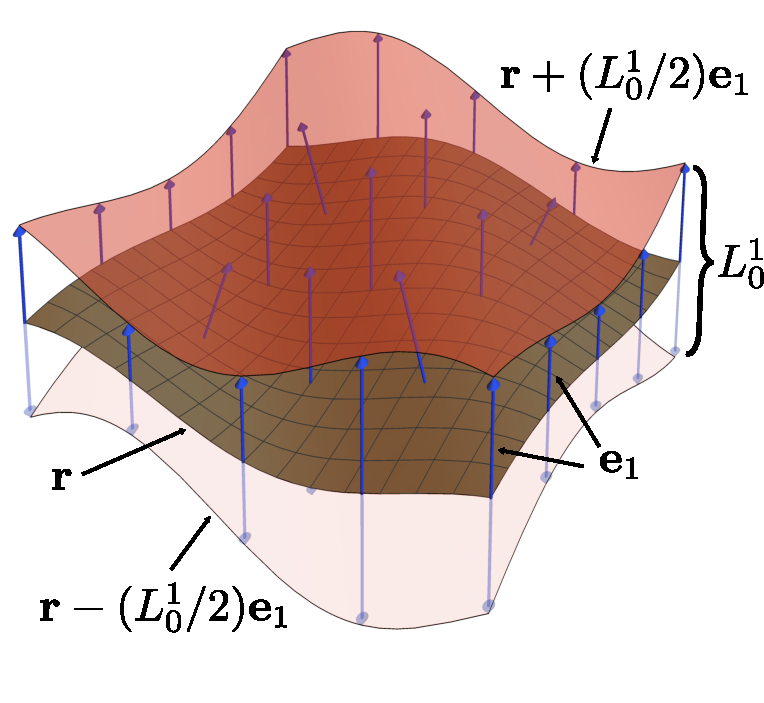
\includegraphics[width=0.8\textwidth]{figs_part2/cosserat_surface/cosserat_kinematics.pdf}
        \caption{The director field $\mathbf{e}_1(u,v)$ (blue arrows) and the midsurface $\mathbf{r}(u,v)$ (brown surface) of the Cosserat surface approximates a thin shell by constraining the material fibres along the director to be fixed. The upper and lower boundaries of the shell (transparent red surfaces) are given by $\mathbf{r}(u,v) \pm (L_0^1 / 2) \mathbf{e}_1(u,v)$ respectively.}
        \label{fig:cosserat surface}
\end{figure}

As we did in Sec.~\ref{sec:Cosserat rod constitutive dynamics} for a slender tube, we will now kinematically approximate the thin shell with a Cosserat system of lower dimensionality. We consider a Cosserat surface, with material base space $M = [0, L_0^2] \times [0, L_0^3]$, and we denote its material coordinates as $(u, v) = (X_2, X_3)$. A single inextensible director $\mathbf{e}_1$ is attached at each material point $(u,v)$. Then, the Cosserat surface approximates the slender body under the kinematic assumption that the fibres along $\mathbf{e}_1$ are rigid bodies. In other words we have
\begin{equation} \label{eq:thin shell kinematic assumption}
\mathbf{x}(\mathbf{X}, t) = \mathbf{r}(t, u, v) + X_1 \mathbf{e}_1.
\end{equation}
where $X_1 \in [-L_0^1/2, L_0^2/2]$ and $\mathbf{r}(t,u,v)$ is the mid-surface. Equation \ref{eq:thin shell kinematic assumption} is illustrated in Fig.~\ref{fig:cosserat surface}. Notably the Cosserat surface only has a single director, as opposed to the two directors of the Cosserat rod. This means that the internal configuration space of the Cosserat surface is $S^2 = SO(3) / SO(2)$ rather than $SO(3)$. However, for the sake of convenience we may add an additional orthonormal director $\mathbf{e}_2$ such that we have a full material frame $E \in SO(3)$. We thus introduce a guage freedom in the physical description of the system, but due to the abelian nature of $SO(2)$ this will not cause any issues in the physical description of the system.

We write $\Phi(t,u,v) = (\mathbf{r}(t, u,v) ; E(t,u,v))$ as before and
\begin{equation}
\xi = N dt + X_u du + X_v dv
\end{equation}
where
\begin{subequations} \label{eq:N X_alpha defs}
\begin{align}
N & = \{ \vec{V}; \vec{\Omega} \} \\
X_u & = \{ \vec{\theta}_u ; \vec{\pi}_u \} \\
X_v & = \{ \vec{\theta}_v ; \vec{\pi}_v \}.
\end{align}
\end{subequations}
From $\Phi^{-1} d \Phi = \xi$ we find
\begin{subequations} 
\begin{align}
d \mathbf{r} & = \mathbf{V} dt + \boldsymbol{\theta}_u du + \boldsymbol{\theta}_v dv  \\
d E & = E \hat{\Omega} dt + E \hat{\pi}_u du + E \hat{\pi}_v dv.
\end{align}
\end{subequations}
and from Eq.~\ref{eq:(summary) geometrised kinematic equations of motion} we find the kinematic equations of motion
\begin{subequations} \label{eq:cosserat surface eom}
\begin{align}
\dot{X}_u & = \mathcal{D}_u N \\
\dot{X}_v & = \mathcal{D}_v N
\end{align}
\end{subequations}
where the spatial reconstruction fields $X_u$ and $X_v$ must obey the spatial integrability conditions
\begin{equation} \label{eq:cosserat surface integrability}
\partial_v X_u = \mathcal{D}_u X_v.
\end{equation}

We now derive the dynamical equations of motion. Carrying out the analogous derivation as we did in Sec.~\ref{sec:Cosserat rod constitutive dynamics}, we find that the kinetic energy density per unit material area is
\begin{equation}
\mathcal{K} = \frac{1}{2} \rho_0 |\vec{V}|^2 + \frac{1}{2} \vec{\Omega}^T \mathbb{I} \vec{\Omega} 
\end{equation}
where $\rho_0 = L_0^1 \rho_0^V$ and $\mathbb{I}$ is the moment-of-inertia of the material frame per unit material area.

From Eq.~\ref{eq:(summary) dynamical equations of motion} we find the dynamical equations of motion
\begin{subequations}  \label{eq:surface dynamical eoms}
\begin{align}
\mathcal{D}_t^* S & = \mathcal{D}_u^* Q^u + \mathcal{D}_v^* Q^v + T \\
n_\alpha Q^\alpha & = 0, \quad \text{on } \partial M.
\end{align}
\end{subequations}
where we sum over $\alpha = u,v$ and $\text{ad}_{\cdot}^*$ was given in Eq.~\ref{eq:SE(3) dual adjoint}, and where
\begin{subequations} \label{eq:S Qu Qv}
\begin{align}
S & = \frac{\partial \mathcal{K}}{\partial N} = \{ \vec{P} ; \vec{L} \}^* \\
Q^u & = \{ \vec{F}^u ; \vec{M}^u \}^* \\
Q^v & = \{ \vec{F}^v ; \vec{M}^v \}^* \\
T & = \{ \vec{f} ; \vec{m} \}^*
\end{align}
\end{subequations}
and $\vec{P} = \rho_0 \vec{V}$ and $\vec{L} = \mathbb{I} \vec{\Omega}$.  Substituting Eq.~\ref{eq:N X_alpha defs} and Eq.~\ref{eq:S Qu Qv} into Eq.~\ref{eq:surface dynamical eoms} we get
\begin{subequations} \label{eq:cosserat surface dynamic eoms}
\begin{align}
D_t \vec{P} & = D_\alpha \vec{F}^\alpha + \vec{f} \label{eq:surface P eom} \\
D_t \vec{L} & = D_\alpha \vec{M}^\alpha + \vec{\theta}_\alpha \times \vec{F}^\alpha + \vec{m} \label{eq:surface L eom} \\
n_\alpha \vec{F}^\alpha & = n_\alpha \vec{M}^\alpha = 0, \quad \text{on } \partial M 
\end{align}
\end{subequations}
where we sum over repeated indices of $\alpha = u, v$, and is consistent with the dynamical equations of motion found in the literature \citep{altenbachCosseratMedia2013}. Repeating the same dimensional arguments as in Sec.~\ref{sec:cosserat 3d bodies}, we can conclude that $\vec{P}$ and $\vec{L}$ have units of momentum and angular momentum per unit material area respectively, and $\vec{F}^\alpha$ and $\vec{M}^\alpha$ force and moment per unit material length respectively. The body force $\vec{f}$ and $\vec{m}$ have units of force and moment per unit material area respectively.

Note that the component $L_1$ of the angular momentum of the material frame is unphysical if the Cosserat surface is seen as an approximate model for a slender shell. For conservative dynamics, this means that $\mathcal{U}$ should not couple to $\pi_1$, which is the rate-of-twist of the material frame around $\mathbf{e}_1$. In general, this entails that $M^\alpha_1 = m^\alpha_1 = 0$.

In the above we have considered a rectangular material base space $M$. However, in general for \textit{open} Cosserat surfaces the material base space can be any bounded and compact subset $M \subset \mathbb{R}^2$. Furthermore, \textit{closed} Cosserat surfaces may have $M = S^2$, in which case the material base space no longer admits global coordinates. The kinodynamical equations of motion above still apply in the case of a closed surface, but they must then be simultaneously and consistently simulated over multiple charts that cover $M$.



%\subsubsection{Kinematic constraints}

%We now eliminate the internal degrees of freedom, such that the system configuration is only specified by $\mathbf{r}(t,u,v) \in \mathbb{E}^3$. We will proceed in a manner analogous to Sec.~\ref{sec:Kinematic constraints and gauge freedoms}.

%Similar to the 

%\citep{olverSurveyMovingFrames2005, felsMovingCoframesPractical1998, felsMovingCoframesII1999, altenbachCosseratMedia2013}




\subsection{Cosserat rods on 2-spheres} \label{sec:Cosserat rods on 2-spheres}

We consider the constitutive dynamics of a generalised Cosserat rod, lying on the $2$-dimensional surface of a sphere $S^2 = \{ \mathbf{x} \in \mathbb{E}^3 \ |\ |\mathbf{x}| = r \}$ where $r$ is the radius of the sphere. Some recent applications of such systems can be found in \citep{mannaEmergentTopologicalPhenomena2019, hsuActivityinducedPolarPatterns2022}. The external configuration space of the rod is thus $S^2 = SO(3) / SO(2)$, and the internal configuration space is $SO(2)$. Let $\mathbf{r}(t,u) = r \mathbf{e}_0(t,u)$ denote the center-line of the rod, where $\mathbf{n}(t,u) \in \mathbb{E}^3$ is a unit-vector, and $u \in [0, L_0],\ t \in [0, T]$. The material frame $E = (\mathbf{e}_1(t,u), \mathbf{e}_2(t,u))$ of the rod are two orthonormal vectors that are tangent to $S^2$ at $\mathbf{r}$, and can be seen as an element of $SO(2)$. We also have that the triad $(\mathbf{n}\ \mathbf{e}_1\ \mathbf{e}_2)$ are mutually orthogonal, and $\mathbf{n}(t,u)$ is normal to $S^1$ at $\mathbf{r}(t,u)$ and $(\mathbf{e}_1\ \mathbf{e}_2)$ forms a basis for $T_{\mathbf{r}(t,u)} S^2$. Furthermore, as the triad forms an orthogonal matrix with unit determinant we can identify it as an element of $SO(3)$, and will thus write $\Phi = (\mathbf{n}\ \mathbf{e}_1\ \mathbf{e}_2)$. The configuration space of the Cosserat rod on the sphere is thus $G = SO(3)$, with kinematic base space $W = [0, T] \times [0, L_0]$ which admits a global basis. As in Ch.~\ref{ch:Cosserat rods} we will distinguish between vectors $\mathbf{v} \in \mathbb{E}^3$ in the fixed frame and vectors $\vec{v} \in \mathbb{R}^3$ in the moving frame, and relate the two as $\vec{v} = \Phi^T \mathbf{v}$. We shall write the components of vectors in the moving frame as $\vec{v} = (v_n, v_1, v_2)$.

We shall write the Maurer-Cartan form as
\begin{equation}
\xi = \hat{N} dt + \hat{X} du
\end{equation}
where $\hat{N}(t,u), \hat{X}(t,u) \in \mathfrak{so}(3)$, and we write
\begin{subequations}
\begin{align}
\vec{N} & = (\Omega_n, -V_2/r, V_1/r)^T \\
\vec{X} & = (\pi_n, -\theta_2/r, \theta_1/r)^T 
\end{align}
\end{subequations}
and
\begin{subequations}
\begin{align}
\vec{V} & = (0, V_1, V_2)^T \\
\vec{\theta} & = (0, \theta_1, \theta_2)^T \\
\vec{\Omega} & = (\Omega_n, 0, 0)^T \\
\vec{\pi} & = (\pi_n, 0, 0)^T.
\end{align}
\end{subequations}
From $\Phi^{-1} d \Phi = \xi$ we find
\begin{subequations}
\begin{align}
d \mathbf{r} & = r d \mathbf{n} = \mathbf{e}_i V_i dt + \mathbf{e}_i \theta_i du \\ 
 & = \mathbf{V} dt + \boldsymbol{\theta} du \nonumber \\
d \mathbf{e}_1 & = (\Omega_n \mathbf{e}_2 - (V_1/r) \mathbf{n}) dt + (\pi_n \mathbf{e}_2 - (\theta_1/r) \mathbf{n}) du \\
d \mathbf{e}_2 & = (-\Omega_n \mathbf{e}_1 - (V_2/r) \mathbf{n}) dt + (-\pi_n \mathbf{e}_1 - (\theta_2/r) \mathbf{n}) du.
\end{align}
\end{subequations}
We can identify $\mathbf{V}(t,u) \in T_{\mathbf{r}(t,u)} S^2$ as the velocity of the center-line at $\mathbf{r}(t,u)$ and likewise $\boldsymbol{\theta}(t,u) \in T_{\mathbf{r}(t,u)} S^2$ as the rate-of-change of the center-line along the material coordinate $u$. We can also identify $\Omega_n(t,u)$ and $\pi_n(t,u)$ as the angular velocity and angular rate-of-rotation of the material frame around $\mathbf{n}$, and thus $\Omega(t,u),  \pi(t,u) \in \mathfrak{so}(2)$.

\begin{figure*} 
    \centering
     
    \begin{subfigure}[b]{0.6\textwidth}  
        \centering 
        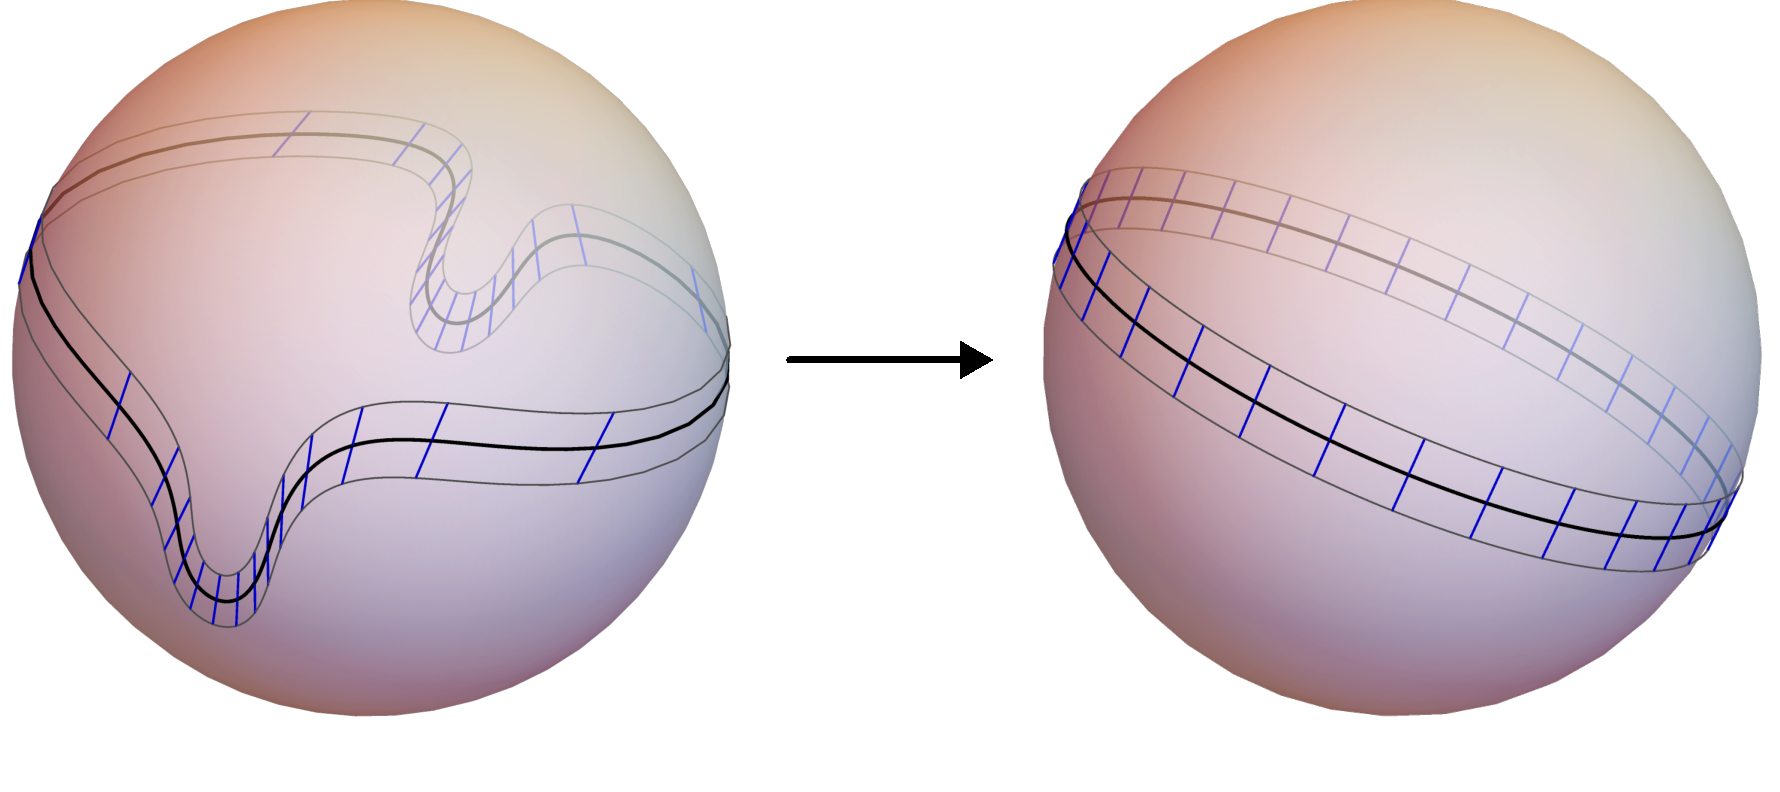
\includegraphics[width=\textwidth]{figs_part2/cosserat_rod_on_spheres/rod_on_sphere.pdf}
        \caption[Overdamped Cosserat rod relaxing to a ground-state]%
        {{\small Overdamped Cosserat rod relaxing to a ground-state}}    
        \label{fig:rod on sphere simulation}
    \end{subfigure}
    \hfill
    \begin{subfigure}[b]{0.32\textwidth}
        \centering
        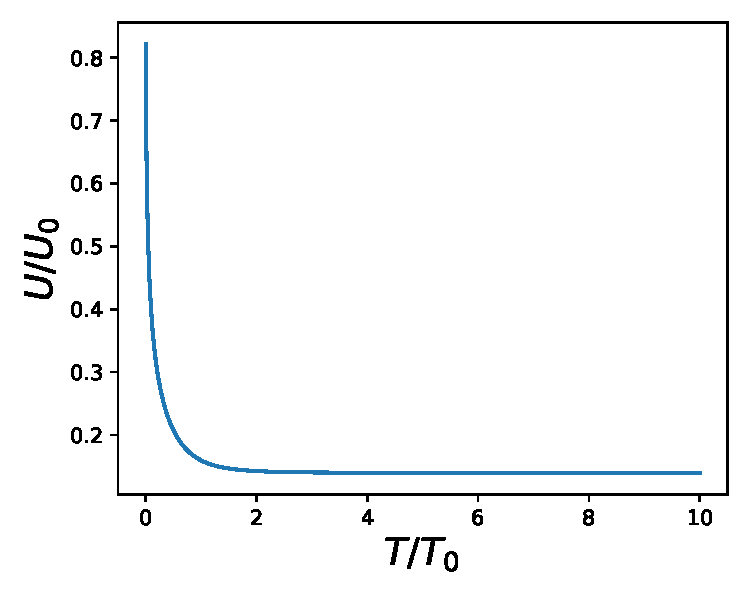
\includegraphics[width=\textwidth]{figs_part2/cosserat_rod_on_spheres/rod_on_sphere_U.pdf}
        \caption[Potential energy]%
        {{\small Potential energy}}    
        \label{fig:rod on sphere U}
    \end{subfigure}    
    
    \caption[  ]
    {\small (a) Overdamped Cosserat rod on $2$-sphere relaxing from a deformed initial configuration (left) to a ground-state (right). Solid black lines are the rod center-lines, and the blue lines are the directors $\mathbf{e}_2$. (b) Potential energy of the Cosserat rod.} 
    \label{fig:rod on sphere}
\end{figure*}

From Eq.~\ref{eq:(summary) geometrised kinematic equations of motion} we can find the kinematic equations of motion
\begin{equation} \label{eq:cosserat rod on sphere kinematic eoms}
\begin{aligned}
\dot{\vec{X}} & = \mathcal{D}_u \vec{N} \\
& = \vec{N}' + \vec{X} \times \vec{N}
\end{aligned}
\end{equation}
using $\overrightarrow{[\hat{X}, \hat{N}]} = \vec{X} \times \vec{N}$. We define the Lagrangian
\begin{subequations} \label{eq:cosserat rod on sphere lagrangian}
\begin{align}
\mathcal{L}(d \Phi) & = \mathcal{K}(\dot{\Phi})) - \mathcal{U}(\Phi') \\
\mathcal{K} & = \frac{1}{2} \rho_0 |\mathbf{V}|^2 + \frac{1}{2} \mathbb{I}_n \Omega_n^2
\end{align}
\end{subequations}
where $\mathcal{U}$ is constitutive potential energy, $\rho_0$ is the mass density per unit material length and $\mathbb{I}_n \in \mathbb{R}$ is the moment-of-inertia per unit material length of the material frame.  In its reduced form, the Lagrangian is
\begin{subequations} \label{eq:cosserat rod on sphere reduced lagrangian}
\begin{align}
\mathcal{\ell}(\xi) & = \mathcal{K}(N) - \mathcal{U}(X) \\
\mathcal{K} & = \frac{1}{2} \rho_0 |\vec{V}|^2 + \frac{1}{2} \mathbb{I}_n \Omega_n^2.
\end{align}
\end{subequations}
The conjugate moment and stress are $\vec{P} = \frac{\partial \ell}{\partial \vec{N}}$ and $\vec{Q} = -\frac{\partial \ell}{\partial \vec{X}}$ respectively, and we get
\begin{subequations} 
\begin{align}
\vec{P} & = (L_n, p_2 r, - p_1 r)^T \\
\vec{Q} & = (M_n, F_2 r, - F_1 r)^T
\end{align}
\end{subequations}
where $\vec{F} = (0, F_1, F_2)^T$ and $\vec{p} = (0, \rho_0 V_1, \rho_0 V_2)^T$ is the force on the center-line and its linear momentum density per unit material length respectively, and where $\vec{M} = (M_n, 0, 0)$ and $\vec{L} = (\mathbb{I}_n \Omega_n, 0, 0)^T$ are the moment on the material frame and its angular momentum per unit material length respectively. From Eq.~\ref{eq:(summary) dynamical equations of motion} we find the dynamical equations of motion
\begin{subequations} \label{eq:rod on 2-sphere dynamical eoms}
\begin{align}
(\partial_t + \hat{N}) \vec{S} & = (\partial_u + \hat{X}) \vec{Q} + \vec{T} \\
Q_\alpha & = 0, \quad u = 0, L_0.
\end{align}
\end{subequations}
where we used $[\text{ad}_X] = \hat{X}$ and $[\text{ad}^*_X] = -[\text{ad}_X]^T$, and where $\vec{T}$ is a generalised body force. In the absence of body forces, and using the definitions of $S, Q, N$ and $X$, we get
\begin{subequations} 
\begin{align} \label{eq:rod on 2-sphere dynamical eoms 2}
\dot{\bar{L}} & = M' + \vec{\theta} \times \vec{F} \\
\dot{\bar{P}} & = D_u \vec{F} - c \vec{\Omega} \times \vec{V} + \frac{1}{r^2} \vec{M} \times \vec{\theta}
\end{align}
\end{subequations}
where $c = \rho_0 + \mathbb{I}_n/r^2$. $\vec{\theta} \times \vec{F}$ is the moment exerted on the material frame due to the force, $\frac{1}{r^2} \vec{M} \times \vec{\theta}$ is the force exerted on the center-line due to the moment, and $- c \vec{\Omega} \times \vec{V}$ can be seen as a Coriolis force that arises due to the rotating frame. Equations \ref{eq:cosserat rod on sphere kinematic eoms} and \ref{eq:rod on 2-sphere dynamical eoms 2} together form a set of equations that completely determine the kinodynamics of the system.

We will now consider the example of `overdamped' Cosserat rod dynamics on the $2$-sphere. We define the frictional body force $\vec{T} = \gamma \vec{N}$, where $\gamma \in \mathbb{R}^{3\times 3}$ is a symmetric and positive-definite matrix, and the constitutive potential
\begin{equation} \label{eq:cosserat rod on sphere U}
\mathcal{U} = \frac{1}{2} \epsilon (\vec{X} - \vec{X}_0)^T \mathsf{K} (\vec{X} - \vec{X}_0)
\end{equation}
where $\vec{X}_0 = (0\ 1\ 0)^T$ and $\mathsf{K} \in \mathbb{R}^{3 \times 3}$ is a positive definite matrix. We take the overdamped limit, eliminating the inertial degrees of freedom $\vec{P} \approx 0$, to get
\begin{subequations} \label{eq:rod on 2-sphere dynamical eoms overdamped}
\begin{align}
\dot{\vec{X}} & = \vec{N}' + \vec{X} \times \vec{N} \\
\gamma \vec{N} & = (\partial_u + \hat{X}) \vec{Q}.
\end{align}
\end{subequations}
Fig.~\ref{fig:rod on sphere} shows the result of a simulation of Eq.~\ref{eq:rod on 2-sphere dynamical eoms overdamped}, depicting the relaxation of an initial deformed state to a ground-state that minimises Eq.~\ref{eq:cosserat rod on sphere U}.

\subsection{Relativistic Cosserat rods} \label{sec:Relativistic Cosserat rods}

Here we derive the kinematic equations of relativistic motion of a Cosserat rod. We work in units where the speed-of-light constant is set to unity $c= 1$. The Minkowski vector space $\mathbb{M}^{1,3}$ is the vector space $\mathbb{R}^4$ equipped with the \textit{Minkowski inner product} $\langle \cdot, \cdot \rangle_M : \mathbb{M}^{1,3} \times \mathbb{M}^{1,3} \to \mathbb{R}$ with signature $(1, 3)$. In other words, given some basis $B = (\mathbf{b}_0, \mathbf{b}_1, \mathbf{b}_2, \mathbf{b}_3)$ for $\mathbb{R}^4$, the \textit{Minkowski metric}
\begin{equation}
\eta_{ij} = \langle \mathbf{b}_i, \mathbf{b}_j \rangle_M
\end{equation}
has $1$ negative eigenvalue and $3$ positive eigenvalues. Henceforth we will assume that the basis is defined such that
\begin{equation} \label{eq:eta diagonalised}
\eta = \text{diag}(-1, 1, 1, 1).
\end{equation}
Any basis that diagonalises $\eta$ as in Eq.~\ref{eq:eta diagonalised} will be called an \textit{orthonormal} basis. A $\mathbf{v} \in \mathbb{M}^{1,3}$ is known as \textit{time-like} if $\langle \mathbf{v}, \mathbf{v} \rangle_M < 0$, \textit{space-like} if $\langle \mathbf{v}, \mathbf{v} \rangle_M > 0$ and \textit{light-like} if $\langle \mathbf{v}, \mathbf{v} \rangle_M = 0$. We can thus identify $\mathbf{b}_0$ as the time-like direction in this basis, and $(\mathbf{b}_1, \mathbf{b}_2, \mathbf{b}_3)$ as the space-like directions.

The \textit{space-time coordinates} $\mathbf{r}(\tau)$ of an observer is a function $\mathbf{r} : \mathbb{R} \to \mathbb{M}^{1,3}$ where $\tau$ is the time measured by clocks co-moving with the observer, known as the \textit{proper time}. The \textit{$4$-velocity} of the observer is given by the time-like vector $\mathbf{U} = \partial_\tau \mathbf{r}$. The \textit{inertial frame} of the observer at proper time $\tau$ is an orthonormal basis $E(\tau) = (\mathbf{e}_0(\tau), \mathbf{e}_1(\tau), \mathbf{e}_2(\tau), \mathbf{e}_3(\tau))$ such that
\begin{equation}
\vec{U} = E^{-1} \mathbf{U} = (1\ 0\ 0\ 0)^T.
\end{equation}
Intuitively, this corresponds to the fact that an observer is always stationary in its own co-moving inertial reference frame. Such a basis can be found by setting $\mathbf{e}_0 = \mathbf{U}$, and the remaining three basis elements $(\mathbf{e}_1, \mathbf{e}_2, \mathbf{e}_3)$ specify the spatial orientation of the observer. Vectors $\vec{v} = E^{-1} \mathbf{v}$ are thus expressed in the inertial frame $E$. We shall use the notation $\tilde{v}$ to refer to the spatial components of $\vec{v}$, such that $\vec{v} = (v_0\ \tilde{v}^T)^T$.


Any two inertial frames $E_1$ and $E_2$ can be related by a \textit{Lorentz transformation}
\begin{equation} \label{eq:E1 E2 lorentz relation}
E_2 = \Lambda E_1
\end{equation}
where $\Lambda \in SO(1, 3)$, and where $SO(1, 3)$ is the \textit{Lorentz group} on $\mathbb{M}^{1,3}$ and is defined as
\begin{equation}
SO(1, 3) = \{ \Lambda \in \mathbb{R}^{4 \times 4} \ |\ \langle \Lambda \mathbf{v}, \Lambda \mathbf{v} \rangle_M = \langle \mathbf{v}, \mathbf{v} \rangle_M\ \forall \mathbf{v} \in \mathbb{M}^{3,1 } \}.
\end{equation}
which is the group of rotations in space and \textit{Lorentz boosts}. The Lorentz group is thus the set of linear transformations that preserves the Minkowski inner product. Combined with the group of translations on $\mathbb{M}^{1,3}$, we have the \textit{Poincaré} group
\begin{equation}
M(1,3) = \left\{
\begin{pmatrix}
1 & \mathbf{0}^T \\
\mathbf{t} & \Lambda
\end{pmatrix} \in \mathbb{R}^{5 \times 5}\ |\ \mathbf{t} \in \mathbb{M}^{1,3},\ \Lambda \in SO(3,1) 
\right\}
\end{equation}
of space-time translations and rotations.

Now consider a continuous `string' of inertial observers with space-time coordinates $\mathbf{r}(\tau, u)$ and inertial frames $E(\tau, u)$, parametrised by $u$. If $\mathbf{e}_0(\tau, u) = \partial_\tau \mathbf{U}(\tau, u)$ then this can be considered a \textit{relativistic} Cosserat rod, where $(\mathbf{e}_1, \mathbf{e}_2, \mathbf{e}_3)$ is here the material frame of the rod. In order to avoid confusing using the word `frame` in reference to both material and inertial frames, we will henceforth refer to the former as the Cosserat cross-section. Given a reference frame $B$ and origin $\mathbf{0} \in \mathbb{M}^{1,3}$, we can write the configuration of the Cosserat rod as
\begin{equation}
\mathcal{F} = \mathcal{F}_0 \Phi
\end{equation}
where
\begin{equation}
\mathcal{F} = (\mathbf{r} ; E ) = \begin{pmatrix}
1 & \mathbf{0}^T \\
\mathbf{r} & E
\end{pmatrix}
\end{equation}
and $\mathcal{F}_0 = (\mathbf{0} ; B)$ and $\Phi = (B^{-1} \mathbf{r} ; B^{-1} \Lambda B)$, and where $\Lambda$ satisfies $E = \Lambda B$. As in Sec.~\ref{sec:Lie group–Lie algebra correspondence}, we now simplify our notation by letting $B = \mathbbm{1}_{4 \times 4}$, such that $\Lambda = E \in SO(1,3)$ and we can thus write $\Phi = \mathcal{F}$. 

We write the Maurer-Cartan form as
\begin{equation}
\xi = N d \tau + X du
\end{equation}
where
\begin{subequations}
\begin{align}
N & = \{ \vec{U} ; O \} = \begin{pmatrix}
0 & \vec{0}^T \\
\vec{U} & O
\end{pmatrix} \\
X & = \{ \vec{\theta} ; \Xi \} = \begin{pmatrix}
0 & \vec{0}^T \\
\vec{\theta} & \Xi
\end{pmatrix} 
\end{align}
\end{subequations}
and $N(\tau, u), X(\tau, u) \in \mathfrak{m}(1,3)$ and $O, \Xi \in \mathfrak{so}(1,3)$. From $\Phi^{-1} d \Phi = \xi$ we find
\begin{subequations}
\begin{align}
d \mathbf{r} & = \mathbf{U} d \tau + \boldsymbol{\theta} du \\
 & = \mathbf{e}_0 d \tau + \boldsymbol{\theta} du \nonumber \\
d \mathbf{e}_\beta & = \mathbf{e}_\alpha O_{\alpha \beta} d\tau + \mathbf{e}_\alpha \Xi_{\alpha \beta} du,\ \alpha,\beta = 0,1,2,3
\end{align}
\end{subequations}
where we used $\mathbf{e}_0 = \mathbf{U}$, which should be seen as a kinematic restriction on the Lie group-valued $\Phi$ (although note that it is not a kinematic restriction from the physical perspective, as real inertial observers always are always stationary with respect to themselves). Because we have parametrised the Cosserat rod with respect to the co-moving inertial frames, we have that $\vec{U}(\tau, u) = (1\ 0\ 0\ 0)^T$. Therefore the kinematic movement of the rod is not specified in $\vec{U}$ as in Sec.~\ref{sec:Geometric Cosserat rod mechanics}, but must instead be encoded in $O$.

The Lie algebra element $O \in \mathfrak{so}(1,3)$ can be written as
\begin{equation}
O = \begin{pmatrix}
0 & \tilde{a}^T \\
\tilde{a} & \hat{\tilde{\Omega}}
\end{pmatrix}
\end{equation}
where $\tilde{a} = (a_1, a_2, a_3)$ and $\hat{\tilde{\Omega}} \in \mathfrak{so}(3)$. Henceforth the tilde will designate spatial $3$-vectors. To interpret these quantities, we first note that
\begin{equation}
\partial_\tau \mathbf{e}_i = \mathbf{e}_i \hat{\tilde{\Omega}}_{ij},\ i=1,2,3
\end{equation}
from which we identify that $\tilde{\Omega}(\tau, u)$ is the angular velocity of the Cosserat cross-section at $u$ in its inertial frame. Secondly, we can compute the \textit{$4$-acceleration} $\mathbf{a} = \partial_\tau^2 \mathbf{r}$ as
\begin{equation} \label{eq:4-acceleration}
\mathbf{a} = \partial_\tau \mathbf{e}_i = \mathbf{e}_i a_i,\ i=1,2,3.
\end{equation}
such that $\vec{a} = E^{-1} \mathbf{a} = (0\ \tilde{a}^T)^T$, which is the correct expression for the co-moving 4-acceleration in special relativistic kinematics \citep[p.~99]{rindlerRelativitySpecialGeneral2001}. We thus see that $\tilde{a}(\tau, u)$ is the acceleration of the Cosserat cross-section at $u$ in its co-moving inertial frame. Therefore the kinematics of the relativistic Cosserat rod is specified by the spatial acceleration $\tilde{a}$ of the center-line and the angular velocity $\tilde{\Omega}$ of the cross-section. This stands in contrast to the non-relativistic Cosserat rod, where we instead specify the velocity of the center-line. We can understand this difference by noting that velocity is \emph{itself} a kinematic degree of freedom in special relativity, in addition to position and orientation. Only the latter two are kinematic degrees of freedom in non-relativistic systems. Mathematically, we have that the relative velocity of an inertial observer with frame $E_1$ with respect to another observer with frame $E_2$ is encoded in the Lorentz transformation that relates the two, as in Eq.~\ref{eq:E1 E2 lorentz relation}. This is therefore the reason why we must specify the \emph{acceleration} of the frame, as opposed to its \emph{velocity}, in the kinematics.

The kinematic equations of motion are given by Eq.~\ref{eq:(summary) geometrised kinematic equations of motion}, from which we find
\begin{subequations}
\begin{align}
\partial_\tau \vec{\theta} & = - O \vec{\theta} + \Xi \vec{U} \\
\partial_\tau \Xi & = \partial_u O + [\Xi, O].
\end{align} 
\end{subequations}
If we let
\begin{equation}
O = \begin{pmatrix}
0 & \tilde{t}^T \\
\tilde{t} & \hat{\tilde{\pi}}
\end{pmatrix}
\end{equation}
then the kinematic equations of motion can be written as
\begin{subequations}
\begin{align}
\partial_\tau \theta_0 & = a_i \theta_i \\
\tilde{D}_\tau \tilde{\theta} & = - \theta_0 \tilde{a} + \tilde{t} \\
\tilde{D}_\tau \tilde{t} & = \tilde{D}_u \tilde{a} \\
\partial_\tau \tilde{\pi} & = \tilde{D}_u \tilde{\Omega}
\end{align} 
\end{subequations}
where $i = 1,2,3$ and $\tilde{D}_\tau = \partial_\tau + \hat{\tilde{\Omega}}$ and $\tilde{D}_u = \partial_u + \hat{\tilde{\pi}}$.

% https://en.wikipedia.org/wiki/Relativistic_mechanics

% https://en.wikipedia.org/wiki/Four-velocity

% https://en.wikipedia.org/wiki/Poincar%C3%A9_group

% https://farside.ph.utexas.edu/teaching/em/lectures/node115.html

% https://physics.stackexchange.com/questions/318361/is-my-interpretation-of-dt-d-tau-correct

% https://en.wikipedia.org/wiki/Relativistic_Lagrangian_mechanics

% https://en.wikipedia.org/wiki/Relativistic_angular_momentum

% https://physics.stackexchange.com/questions/520222/when-we-calculate-the-relativistic-angular-momentum-of-a-particle-in-the-directi

%\subsection{Nematic materials}

%$RP^2 \cong S^2/~$

%https://math.stackexchange.com/questions/1391724/real-projective-plane-is-same-as-identifying-antipodal-boundary-points-of-the-2

% https://math.stackexchange.com/questions/2876529/how-can-a-representation-of-so3-be-more-than-3-dimensional

% https://math.stackexchange.com/questions/4268711/why-does-a-space-of-symmetric-traceless-tensors-form-an-irreducible-representati

% https://math.stackexchange.com/questions/3626821/spherical-harmonics-and-irreducible-representations-of-so2-and-so3

% http://visuallietheory.blogspot.com/2013/07/real-representations-of-lie-algebra.html

\subsection{The $O(N)$ non-linear $\sigma$ model} \label{sec:The O(3) non-linear sigma model}

Here we give an example of the geometrisation programme applied to a field theory. We consider a field $\vec{n} : W \to S^N \subset \mathbb{R}^N$, where $W$ is the base space and $\vec{n}$ is a unit-vector in $\mathbb{R}^N$ for all $p \in W$. We call $S^N \subset \mathbb{R}^N$ the \textit{target manifold} of the field theory. We let $W = \mathbb{M}^{1,d}$, which is the $(d+1)$-dimensional Minkowski space, although what follows is easily generalisable to Euclidean space or any arbitrary base space.  
 We define coordinates $(t, u^1, u^2, \dots, u^d)$ on $\mathbb{M}^{1,d}$, and we will write partial derivatives as $\partial_\gamma,\ \gamma=0,1,\dots,d$, where $\partial_0 = \frac{\partial}{\partial t}$ and $\partial_\alpha = \frac{\partial}{\partial u^\alpha},\ \alpha=1,\dots,d$.

The \textit{$O(N)$ non-linear $\sigma$ model} \citep{ketovQuantumNonlinearSigmaModels2013} is defined by the Lagrangian density
\begin{equation} \label{eq:O(N) model}
\mathcal{L} = \frac{1}{2} \eta^{\gamma \kappa} (\partial_\gamma \vec{n})^T (\partial_\kappa \vec{n}) 
\end{equation}
which is expressed in some local coordinate chart of $\mathbb{M}^{1,d}$, where $\eta$ is the Minkowski metric on $\mathbb{M}^{1,d}$ with signature $(1,d)$.

Let the $SO(N)$-valued field $\Phi : \mathbb{M}^{1,d} \to SO(3)$ satisfy $\vec{n} = \Phi \vec{n}_0$ where $\vec{n}_0 \in S^N$ is some constant reference vector. We can then rewrite Eq.~\ref{eq:O(N) model} as
\begin{equation}
\mathcal{L} = \frac{1}{2} \eta^{\gamma \kappa} (\partial_\gamma \Phi \vec{n}_0)^T (\partial_\kappa \Phi  \vec{n}_0) 
\end{equation}
Now, we have
\begin{equation}
\begin{aligned}
(\partial_\gamma \Phi \vec{n}_0)^T (\partial_\kappa \Phi  \vec{n}_0) & = (\Phi^{-1} \partial_\gamma \Phi \vec{n}_0)^T (\Phi^{-1} \partial_\kappa \Phi  \vec{n}_0) \\
& = (\hat{Z}_\gamma \vec{n}_0)^T (\hat{Z}_\kappa \vec{n}_0)
\end{aligned}
\end{equation}
for all $\gamma,\kappa = 1,\dots, d$, where we have defined $\hat{Z}_\gamma = \Phi^{-1} \partial_\gamma \Phi \in \mathfrak{so}(N)$. As before we will  be making use of the hat-map to convert anti-symmetric $3\times 3$-matrices $\hat{Z}_\gamma$ to $3$-vectors $\vec{Z}_\gamma$. Let us now assume that the coordinates are defined such that $\eta = \text{diag}(-1, 1, \dots, 1)$, where the speed-of-light constant has been set to unity $c=1$. The Lagrangian then has a reduced form
\begin{equation}
\ell(\xi) = - \frac{1}{2} \vec{N}^T \mathsf{N}_0 \vec{N} + \frac{1}{2} \sum_{\alpha=1}^d \vec{X}_\alpha^T \mathsf{N}_0 \vec{X}_\alpha
\end{equation}
where $\vec{N} = \vec{Z}_0$ and $\vec{X}_\alpha = \vec{Z}_\alpha,\ \alpha = 1, \dots, d$ and $\mathsf{N}_0 = \hat{n}_0^T \hat{n}_0$ and we have used $|\hat{Z}_\gamma \vec{n}_0 | = |\vec{Z}_\gamma \times  \vec{n}_0 | = | \hat{n}_0 \vec{Z}_\gamma  |$.

We can then readily apply the geometrisation programme to the system, to get the field equations of motion
\begin{subequations} 
\begin{align}
\partial_t \vec{X}_\alpha & = (\partial_\alpha + \hat{X}_\alpha) N \\
(\partial_t + \hat{N}) \vec{S} & = \sum_{\alpha=1}^d (\partial_\alpha + \hat{X}_\alpha) \vec{Q}^\alpha  \label{eq:dynamic field equations}
\end{align}
\end{subequations}
where $\vec{N} = \vec{Z}_0$, $\vec{X}_\alpha = \vec{Z}_\alpha,\ \alpha = 1, \dots, d$, $S = \frac{\partial \ell}{\partial N}$ and $Q^\alpha = \frac{\partial \ell}{\partial X_\alpha}$. The spatial reconstruction fields $X_\alpha$ must satisfy the spatial integrability conditions
\begin{equation}
\partial_\beta X_\alpha = \mathcal{D}_\alpha X_\beta
\end{equation}
at all times $t$, where $\alpha = 1, \dots, d-1$ and $\beta = \alpha+1, \dots, d$.

Note that only two of the three components of $S$ are independently determined by Eq.~\ref{eq:dynamic field equations}, as $\mathsf{N}_0$ is only a rank 2 matrix. To see this let $\vec{n}_0 = (1\ 0\ 0)^T$ such that $\mathsf{N}_0 = \text{diag}(0,1,1)$. We then have that $\vec{S} = (0, N_2, N_3)$ and $Q^\alpha = (0, X_2, X_3)$. This reflects the fact that rotations of $\vec{n}$ around its own axis is a gauge freedom in our formulation of the $O(N)$ non-linear $\sigma$ model.


\begin{comment}

----

On the section for dynamics of homogeneous spaces, recreate the derivation in \citep{poincareFormeNouvelleEquations1901} but where you use your generalised Lagrange-D'Alembert principle.

----

You'll be writing down the Lagrange-Dalembert for the general case of submanifolds of Lie groups. You'll have to motivate what it even means to have an action principle for an abstract system like this where you have not specified exactly what the system even represents. The point is that \textit{if} you have specified some d'Alembert Lagrange dynamics on the level of the Lie group, then it is the case that the reduced d'Alemebert Lagrange dynamics are \textit{equivalent}.

Therefore, programmatically, we can say that to specify the dynamics we first formulate it on the Lie group (which is essentially the program in \citep{alvesMethodVirtualPower1993}), which is often more straightforward and intuitive, and then we reduce it to a Lie algebraic description.

So we start with something like this (have to find the correct version)

\begin{equation}
\int_W ( P_i \delta \dot{q}_i - Q_i \delta q_i) dt \wedge du + \int \mathbf{T}(\delta \Phi) dt \wedge du 
\end{equation}

Programatically, the steps are:

\begin{itemize}
\item Specify the system in some coordinatised way. In the case of a slender tube, we identified that the system can be kinematically approximated as a center-line with a material frame attached, which is the Cosserat rod.

\item Write down the kinetic energy, and the constitutive and body forces and moments acting on it, and write down the Lagrange-D'Alembert principle.

\item If it is the case, identify an isomorphism between the system configuration space and a Lie group. 

\item Using the MC form, derive the kinematic equations of motion.

\item In the Lie group-level dynamics, write the kinetic energy in terms of the Lie algebra. Likewise constrain the constitutive force to be a function of the Lie algebra. If you have a constitutive potential, you need to write it in terms of the Lie algebra. Body forces can in general be functions of both Lie group and Lie algebra. Thus write down the reduced Lagrange-D'Alembert principle.

\item From the reduced Lagrange-D'Alembert principle, derive the dynamical equations of motion.

\item If the configuration space is a homogeneous space, the same steps above apply. The final step is to choose an adapted frame, a gauge choice, with which the constrain the kinematics.

\end{itemize}

Perhaps these steps should have their own section, where I go through each step as a subsection and I provide examples.

\end{comment}








\chapter{Geometric numerical integrators} \label{ch:Geometric numerical integrators}

In numerics, the general class of systems considered in Ch.~\ref{ch:Geometric continuum mechanics on homogeneous configuration spaces} are simulated by integrating the kinodynamic equations of motion, which were stated in full in Eq.~\ref{eq:combined, eoms}. One of the simplest methods to use is the Forward-Euler integrator (FEI), wherein the equations are linearised by means of a uniform discretisation in time. However, the Lie group-geometric intricacies of Eq.~\ref{eq:combined, eoms} are lost if such a scheme is applied. In particular, the adjoint action of the Lie group $G$ is prominent in the equations of motion, where $G$ is either the symmetry group of the configuration space or the configuration space itself. In this chapter we develop numerical integrators that are built around the properties of $G$. As we show in Sec.~\ref{sec:lie group integrators applications}, the resulting \textit{geometric} numerical integrators preserve the spatial integrability conditions Eq.~\ref{eq:combined, spatial integrability}.

The equations of motion we consider in this text can all be be put into the form
\begin{equation} \label{eq:general class of matrix equations}
\partial_t x = F + A x
\end{equation}
where $x = x(t,\mathbf{u}) \in \mathbb{R}^n$ is the state of the system, and $F$ is a $\mathbb{R}^n$-valued drift-field and $A$ a $\mathbb{R}^{n \times n}$-valued linear operator acting on the components of $x$. In general, $F$ and $A$ can be dependent on $x$ as well as its derivatives $\partial_\alpha x, \partial^2_\alpha x$, including higher-order derivatives. Given an initial condition $x(t_0) = x_0$ and $F_0 = f(x_0, \partial_\alpha x |_{x = x_0}, \dots)$ and $A_0 = A(x_0, \partial_\alpha x |_{x = x_0}, \dots)$, then we can approximate $x(t_0 + \Delta t)$ as
\begin{equation} \label{eq:FE scheme}
	x(t_0 + \Delta t, \mathbf{u}) \approx F_0 \Delta t + A_0 x_0 \Delta t.
\end{equation}
which is an approximate short-time propagator Eq.~\ref{eq:general class of matrix equations}. This is the Forward-Euler integration scheme, using which we can numerically approximate solutions to Eq.~\ref{eq:general class of matrix equations} on a uniform time-grid $t_i = i \Delta t$. Implicitly we have assumed that $f$ and the product $A x_0$ are constant in the time-interval $[t_0, t_0 + \Delta t]$ in Eq.~\ref{eq:FE scheme}. We now relax the latter assumption, approximating Eq.~\ref{eq:general class of matrix equations} as
\begin{equation} \label{eq:general class of matrix equations}
\partial_t x \approx F_0 + A_0 x,\ \quad t \in [t_0, t_0 + \Delta t].
\end{equation}
where $x(t_0) = x_0$. The right-hand side can be solved analytically \citep{haleOrdinaryDifferentialEquations2009}, such that we get the alternative short-time propagator
\begin{equation} \label{eq:general lie group integrator}
	x(t_0 + \Delta t, \mathbf{u}) \approx e^{\Delta t A_0} x_0 + \left( \int_0^{\Delta t} e^{(\Delta t - \Delta t') A_0} d \Delta t' \right) F_0,
\end{equation}
which provides an alternative to the FEI.

Now, let $\mathfrak{g}$ be a a Lie algebra with representation $\rho : \mathfrak{g} \to \mathfrak{gl}(V)$, where $V$ is an $n$-dimensional vector space and $\mathfrak{gl}(V)$ is the Lie algebra of the general linear group. If we recast Eq.~\ref{eq:general class of matrix equations} such that $A$ is an element of the given Lie algebra representation (that is, $A \in \rho(\mathfrak{g})$), then $x$ takes values in the vector space $V$ that the Lie algebra is acting on. Furthermore, the drift-field is now a function $F : V \to V$, and should be considered to take values in $\mathfrak{t}$, the Lie algebra of the \textit{translation group}\footnote{Note that as the translation group is abelian, we have that it is isomorphic with its Lie algebra $\mathfrak{t}(V) \cong T$.} $T$ acting on $V$. The right-hand side of Eq.~\ref{eq:general class of matrix equations} can thus be seen as a combination of a translation $F$ and the $\mathfrak{g}$-action $A$ on the $V$-valued $x$. Therefore, the linear map
\begin{equation}
	x \mapsto F + Ax
\end{equation}
can \textit{itself} be seen as a representation of the product Lie algebra $\mathfrak{t} \times \mathfrak{g}$. This can be seen explicitly by rewriting Eq.~\ref{eq:general class of matrix equations} as
\begin{equation} \label{eq:recast matrix equation}
	\partial_t \begin{pmatrix}
		1 \\ x
	\end{pmatrix} = M \begin{pmatrix}
		1 \\ x
	\end{pmatrix}
\end{equation} 
where
\begin{equation}
	M = \begin{pmatrix}
		0 & 0 \\
		F & A
	\end{pmatrix},
\end{equation}
where we identify $M$ as a representation of $\mathfrak{t} \times \mathfrak{g}$.

 Now, if we repeat the same derivation we did previously to get a short-time propagator for Eq.~\ref{eq:recast matrix equation}. Let $x(t_0) = x_0$ and $M_0 = M|_{x = x_0}$, we then have
\begin{equation} \label{eq:general lie group integrator 2}
	\begin{pmatrix}
		1 \\ x(t + \Delta t), \mathbf{u})
	\end{pmatrix} \approx e^{\Delta t M_0} \begin{pmatrix}
		1 \\ x_0
	\end{pmatrix}.
\end{equation}
Recall that the exponential map of a Lie algebra representation yields a representation of the corresponding Lie group. Therefore, therefore we have that $e^{\Delta t M_0}$ is a representation of the Lie group product $T \times G$. Now, note that Eq.~\ref{eq:general lie group integrator 2} must be equivalent Eq.~\ref{eq:general lie group integrator}. This tells us that the right-hand side of Eq.~\ref{eq:general class of matrix equations} can be seen as the infinitesimal action of the Lie algebra $\mathfrak{t} \times \mathfrak{g}$ on the $V$-valued $x$, via the given representation. Eq.~\ref{eq:general lie group integrator} thus ensures, using the exponential map $\exp : \mathfrak{t} \times \mathfrak{g} \to T \times G$, that we properly integrate the infinitesimal action from the Lie algebra to the corresponding Lie group $T \times G$. In this setting, the integrator Eq.~\ref{eq:general lie group integrator} is known as a \textit{Lie group integrator} (LGI) \citep{celledoniIntroductionLieGroup2014c, owrenLieGroupIntegrators2016, iserlesLiegroupMethods2005, celledoniLieGroupIntegrators2022}.

Both the FEI and the LGI will suffer numerical errors. However, the errors of the former will accrue in such a way that the `effective' action of $F$ and $A$ on $x$ does not exponentiate to a well-defined action on the Lie group-level. On the other hand, the LGI is defined so that errors accrue \textit{in the Lie group itself}.

%We thus see that the integrator we derived in Eq.~\ref{eq:general lie group integrator} can be seen as the result of exponentiating the action of $\mathfrak{t} \times \mathfrak{g}$ to its corresponding Lie group $T \times G$, via the exponential map $\exp : \mathfrak{t} \times \mathfrak{g} \to T \times G$. 

%In other words the right-hand side of Eq.~\ref{eq:general class of matrix equations} can thus be seen as the infinitesimal action of the Lie algebra $\mathfrak{t} \times \mathfrak{g}$ on the $V$-valued $x$, via the given representation. Eq.~\ref{eq:general lie group integrator} thus ensures, using the exponential map, that we properly integrate the infinitesimal action from the Lie algebra to the Lie group $T \times G$, which the FE fails to do in general.

In Sec.~\ref{sec:Geometric integrators for general configuration spaces} we will use the results above to derive Lie group integrators for the general class of $G/H$-configured systems considered in Ch.~\ref{ch:Geometric continuum mechanics on homogeneous configuration spaces}. We will then present results for the specific cases of $SO(3)$- and $SE(3)$-valued configuration spaces in Sec.~\ref{sec:Geometric integrators for SO(3)-valued configuration spaces} and Sec.~\ref{sec:Geometric integrators for SE(3)-valued configuration spaces} respectively. The results of these latter two sections also apply for systems with a configuration space that is a homogeneous space for which $SO(3)$ or $SE(3)$ is the symmetry group. Sec.~\ref{sec:lie group integrators applications} we show some numerical results for the Cosserat rod and Cosserat sheet, simulated using the geometric integrators.

\section{Geometric integrators for general configuration spaces} \label{sec:Geometric integrators for general configuration spaces}

We consider a system with a $d$-dimensional material base space $M$ and configuration space $G/H$, where $G$ is an $n$-dimensional Lie group with Lie algebra $\mathfrak{g}$ and $H \subset G$ is a Lie subgroup. The kinodynamic equations of motion of the system are given in Eq.~\ref{eq:combined, eoms}, which can be put into the form of Eq.~\ref{eq:general class of matrix equations} by setting
\begin{subequations} \label{eq:rewritten kinodynamic eoms}
	\begin{align}
		\partial_t X_\alpha  & = F_\alpha + A X_\alpha \label{eq:rewritten kinematic eom} \\
		\partial_t S & = H + B S \label{eq:rewritten dynamic eom}
	\end{align}
\end{subequations}
where $\alpha = 1, \dots, d$ and
\begin{subequations} \label{eq:F H defs}
	\begin{align}
		F_\alpha & = \partial_\alpha N \\
		H & = \mathcal{D}^*_\alpha Q^\alpha + T
	\end{align}
\end{subequations}
and $A = - \text{ad}_N$, $B = - \text{ad}^*_N$, where we used $\text{ad}_X N = - \text{ad}_N X$. We assume that all quantities are expressed in a non-dimensionalised form . Now, as per the discussion in the introduction of this chapter, we recognise that the vector spaces in which $X$ and $S$ take values in are $\mathfrak{g}$ and $\mathfrak{g}^*$ respectively. Furthermore, $f$ and $h$ are translations acting on  $\mathfrak{g}$ and $\mathfrak{g}^*$ respectively, and $A$ and $B$ are elements of the \textit{adjoint representation} of $\mathfrak{g}$ and its corresponding dual representation, respectively. The adjoint representation $\text{ad} : \mathfrak{g} \to \mathfrak{gl}(\mathfrak{g})$ maps Lie algebra elements to linear maps on the Lie algebra itself. We will consider $X$ and $N$ in their fundamental matrix representation $X,N \in \mathbb{R}^{m \times m}$ for some $m$, and we write their indices as $X_{ij}$ and $N_{ij},\ i,j=1,\dots, m$.

From Eq.~\ref{eq:general lie group integrator} we find the short-term propagators
\begin{subequations} \label{eq:kinodynamic short term propagators}
	\begin{align}
		X_\alpha(t_0 + \Delta t, \mathbf{u}) & \approx e^{- \Delta t\ \text{ad}_N} X_0
			+ \left( \int_0^{\Delta t} e^{-(\Delta t - \Delta t') \text{ad}_N} d \Delta t' \right) F_{\alpha,0} \\
		S(t_0 + \Delta t, \mathbf{u}) & \approx e^{- \Delta t\ \text{ad}^*_N} S_0
			+ \left( \int_0^{\Delta t} e^{- (\Delta t - \Delta t') \text{ad}^*_N} d \Delta t' \right) H_0. \label{eq:S short-term propagator}
	\end{align}
\end{subequations}
To use the short-term propagators the matrix exponentials and the integrals must be evaluated. Though as $\text{ad}_N \in \mathbb{R}^{m^2 \times m^2}$ in matrix form, numerically evaluating the exponentials of adjoint representations can be expensive. However, we can more efficiently compute them using the identity
\begin{equation}
	\text{Ad}_{e^Y} = e^{\text{ad}_Y}
\end{equation}
for any $Y \in \mathfrak{g}$, and $\text{Ad}$ is the adjoint action of the Lie group, defined as
\begin{equation} \label{eq:adjoint action 2}
\text{Ad}_g Y = g Y g^{-1}
\end{equation} 
for any $g \in G$. We therefore have that, using $(e^{Y})^{-1} = e^{-Y}$
\begin{subequations} \label{eq:exp expressions for kinematic eom}
	\begin{align}
		e^{-\Delta t\ \text{ad}_N} X_{\alpha, 0} & = e^{- \Delta t N} X_{\alpha, 0} e^{\Delta t N} \\
		\left( \int_0^{\Delta t} e^{-(\Delta t - \Delta t') \text{ad}_N} d \Delta t' \right) F_{\alpha, 0} & = \int_0^{\Delta t} e^{- (\Delta t - \Delta t') N} F_{\alpha, 0} e^{(\Delta t - \Delta t') N}  d \Delta t'
	\end{align}
\end{subequations}
where the right-hand sides are now expressed in terms of the exponentials of the Lie algebra elements, which are computationally more convenient to compute. To find the equivalent expressions for Eq.~\ref{eq:S short-term propagator}, note that from $e^{\text{ad}^*_Y} = e^{(\text{ad}_Y)^T} = (e^{\text{ad}_Y})^T$ we have that $e^{\text{ad}^*_Y} = (\text{Ad}_{ e^Y })^T$. To find the transpose of the adjoint action, we can write Eq.~\ref{eq:adjoint action 2} in index form $(\text{Ad}_g Y)_{ij} = (\text{Ad}_g)_{ik, jl} Y_{kl}$, where $(\text{Ad}_g)_{ik, jl} = g_{ik} g^{-1}_{lj}$, summing over repeated indices. Then $(\text{Ad}_g)^T_{ik, jl} = (\text{Ad}_g)_{jl, ik} = g_{jl} g^{-1}_{ki}$ such that
\begin{equation} \label{eq:adjoint action 2}
(\text{Ad}_g)^T Z = (g^{-1})^T Z g^T
\end{equation} 
for any $Z \in \mathfrak{g}^*$ and $g \in G$. We thus find that
\begin{subequations} \label{eq:exp expressions for dynamic eom}
	\begin{align}
		e^{-\Delta t\ \text{ad}^*_N} S_0 & = (e^{\Delta t N})^T S_0 (e^{- \Delta t N})^T \\
		\left( \int_0^{\Delta t} e^{-(\Delta t - \Delta t') \text{ad}^*_N} d \Delta t' \right) H_0 & = \int_0^{\Delta t} (e^{(\Delta t - \Delta t') N})^T H_0 (e^{-(\Delta t - \Delta t') N})^T d \Delta t' \nonumber \\
		& = \left( \int_0^{\Delta t} (e^{-(\Delta t - \Delta t') N}) H_0^T (e^{(\Delta t - \Delta t') N}) d \Delta t' \right)^T 
	\end{align}
\end{subequations}
Comparing Eqs.~\ref{eq:exp expressions for kinematic eom} and \ref{eq:exp expressions for dynamic eom}, we see that they can be evaluated using the same sequence of calculations. We define
\begin{equation}
	\mathscr{E}_G(\Delta t, N, Y) = \int_0^{\Delta t} e^{-(\Delta t - \Delta t') N} Y e^{(\Delta t - \Delta t') N} d \Delta t'
\end{equation}
where $N,Y \in \mathbb{R}^{m \times m}$ are constant matrices, such that we can rewrite Eq.~\ref{eq:kinodynamic short term propagators} as
\begin{subequations} \label{eq:kinodynamic short term propagators}
	\begin{align}
		X_{\alpha}(t_0 + \Delta t, \mathbf{u}) & \approx e^{- \Delta t N} X_{\alpha, 0} e^{ \Delta t N} + \mathscr{E}_G(\Delta t, N, F_{\alpha, 0}) \label{eq:X propagator} \\
		S(t_0 + \Delta t, \mathbf{u}) & \approx (e^{\Delta t N})^T S_0 (e^{-\Delta t N})^T + \mathscr{E}_G(\Delta t, N, H_0^T)^T, \label{eq:S propagator}
	\end{align}
\end{subequations}
where the transposes in Eq.~\ref{eq:S propagator} can be understood by recalling the matrix representation of the dual Lie algebra $\mathfrak{g}^* = \{ Y^T\ :\ Y \in \mathfrak{g} \}$ (see Eq.~\ref{eq:(summary) generalised conjguate momentum}). We can thus treat Eq.~\ref{eq:S propagator} in a manner identical to Eq.~\ref{eq:X propagator} by taking the transpose, to get
\begin{equation}
	S^T(t_0 + \Delta t, \mathbf{u}) \approx e^{-\Delta t N} S^T_0 e^{\Delta t N} + \mathscr{E}_G(\Delta t, N, H_0^T).
\end{equation}
We see that in order to evaluate the short-term propagator we need to compute $e^{- \Delta t N}$, $\mathscr{E}_G(\Delta t, N, F_0)$ and $\mathscr{E}_G(\Delta t, N, H_0^T)$. For many Lie groups, the exponential map is known in closed-form such that $e^{- \Delta t N}$ can be computed efficiently. If this is not the case, it can be approximated using
\begin{equation}
e^{Y} = \sum_{k=0}^\infty \frac{1}{k!} Y^k
\end{equation}
up to arbitrary precision by truncating the sum. Once an expression for $e^{- \Delta t N}$ has been found (whether it is analytic or approximate), we must compute $\mathscr{E}_G(\Delta t, N, Y)$. In principle this can be done using numerical quadrature, but in Sec.~\ref{sec:Geometric integrators for SO(3)-valued configuration spaces} and Sec.~\ref{sec:Geometric integrators for SE(3)-valued configuration spaces} we derive their closed-form expressions for $SO(3)$- and $SE(3)$-configured systems. 

\section{Geometric integrators for $SO(3)$-configured system} \label{sec:Geometric integrators for SO(3)-valued configuration spaces}

Here we construct the short-term propagator for $SO(3)$-configured systems. The results also apply to systems with homogeneous configuration spaces, like $S^2$, on which $SO(3)$ is the associated symmetry group. The closed-form expression for the exponential map $\exp_{SO(3)} : \mathfrak{so}(3) \to SO(3)$ is \citep{blancoTutorialSETransformation}
\begin{equation}
	\exp_{SO(3)}(\hat{Y}) = \mathbbm{1}_{3}+\frac{\sin|\vec{Y}|}{|\vec{Y}|}\hat{Y}+\frac{1-\cos|\vec{Y}|}{|\vec{Y}|^{2}}\hat{Y}^{2}
\end{equation}
where $\vec{Y} \in \mathbb{R}^3$ and $\hat{Y} \in \mathfrak{so}(3)$ is given by the hat map Eq.~\ref{eq:hat map}. Now using the identity $R \hat{Y} R^{-1} = \widehat{R \vec{Y}}$ for any $R \in SO(3)$, we have
\begin{equation} \label{eq:E-map SO(3)}
	\mathscr{E}_{SO(3)}(\Delta t, \hat{N}, \vec{Y}) = \Delta t \mathscr{B}(- \Delta t \hat{N}) \vec{Y} 
\end{equation}
where
\begin{equation} \label{eq:SO(3) exp map}
\begin{aligned}
	\mathscr{B}(\hat{Y}) & = \int_0^1  \exp_{SO(3)} ( \alpha \hat{Y} ) d \alpha \\
	& = \mathbbm{1}_{3}+\frac{1-\cos|\vec{Y}|}{|\vec{Y}|^{2}}\hat{Y}+\frac{|\vec{Y}|-\sin|\vec{Y}|}{|\vec{Y}|^{3}}\hat{Y}^{2}.
\end{aligned}
\end{equation}
For convenience we have let $\mathscr{E}_{SO(3)}(\Delta t, \hat{N}, \hat{Y}) \in \mathbb{R}^3$ using the inverse hat-map. The short-term propagator can then be written as
\begin{subequations} \label{eq:SO(3) kinodynamic short term propagators}
	\begin{align}
		\vec{X}_{\alpha}(t_0 + \Delta t, \mathbf{u}) & \approx \exp_{SO(3)}( - \Delta t \hat{N} ) \vec{X}_{\alpha, 0} + \mathscr{E}_{SO(3)}(\Delta t, \hat{N}, \vec{F}_{\alpha, 0}) \\
		\vec{S}(t_0 + \Delta t, \mathbf{u}) & \approx \exp_{SO(3)}( - \Delta t \hat{N} ) \vec{S}_0 + \mathscr{E}_{SO(3)}(\Delta t, \hat{N}, \vec{H}_0).
	\end{align}
\end{subequations}
where $\vec{F}_{\alpha, 0}$ and $\vec{H}_0$ are computed using Eq.~\ref{eq:F H defs}. As the exponential map Eq.~\ref{eq:SO(3) exp map} is ill-conditioned for  small $|\vec{Y}|$, it is often necessary to Taylor expand $\exp_{SO(3)} ( \alpha \hat{Y} )$ and $\mathscr{E}_{SO(3)}(\Delta t, \hat{N}, \vec{Y})$ to at least $O(|\vec{Y}|^6)$ when $|\vec{Y}| < 0.1$.

\section{Geometric integrators for $SE(3)$-configured systems} \label{sec:Geometric integrators for SE(3)-valued configuration spaces}

Here we construct the short-term propagator for $SE(3)$-configured systems. The results also apply to systems with homogeneous configuration spaces, like $\mathbb{E}^3$, on which $SE(3)$ is the associated symmetry group. We will only present the results here. See App.~\ref{app:Detailed derivation of the SE(3) short-time propagator} for detailed derivations. As for the Cosserat systems, we write the kinematic and dynamical quantities of the equations of motion as $X_\alpha = \{ \vec{\theta}_\alpha, \vec{\pi}_\alpha \}$, $N = \{ \vec{V} ; \vec{\Omega} \}$, $S = \{ \vec{P} ; \vec{L} \}^*$ and $Q = \{ \vec{F} ; \vec{M} \}^*$. All quantities are assumed to be expressed in a non-dimensionalised form.

The closed form expression for the exponential map $\text{exp}_{SE(3)} : \mathfrak{se}(3) \to SE(3)$ is \citep{blancoTutorialSETransformation}
\begin{equation} \label{eq:SE(3) exp map}
	\exp_{SE(3)}(Y) = \begin{pmatrix}
		1 & \vec{0}^T \\
		\mathscr{B}(\hat{m}) \vec{a} & \exp_{SO(3)}(\hat{m})
	\end{pmatrix}.
\end{equation}
In App.~\ref{app:Detailed derivation of the SE(3) short-time propagator} we show that
\begin{equation} \label{eq:E thingie SE(3) result}
	\mathscr{E}_{SE(3)}(\Delta t, N, Y)  = \begin{pmatrix}
		0 & \vec{0}^T \\
		\circled{1} + \vec{r}(\Delta t, \vec{m}, \vec{V}) & \circled{2}
		\end{pmatrix}
\end{equation}
where
\begin{subequations}
	\begin{align}
		\circled{1} & = \Delta t \mathscr{B}( - \Delta t \hat{\Omega}) \vec{a} \\
		\circled{2} & = \mathscr{E}_{SO(3)}(\Delta t, \hat{\Omega}, \hat{m}) \\
		\vec{r}(\Delta t, N, \vec{m}) & = \frac{1}{|\vec{\Omega}|^2} \sum_{i,j=1}^{3} R_{ij} \bar{\Omega}^{i-1} \hat{m} \bar{\Omega}^{j-1} \vec{V}
	\end{align}
\end{subequations}
where $\bar{\Omega} = \hat{\Omega} / |\vec{\Omega}|$ and
\footnotesize
\begin{equation} \label{eq:geometric integrator R matrix}
\begin{aligned}
	& R = \psi^{-2} \int_0^1 d\alpha P =  \\
	& \begin{pmatrix}
\frac{\psi^{2}}{2} & - \psi + \sin{\left(\psi \right)} & \frac{\psi^{2}}{2} + \cos{\left(\psi \right)} - 1\\
- \psi \cos{\left(\psi \right)} + \sin{\left(\psi \right)} & - \frac{\left(\cos{\left(\psi \right)} - 1\right)^{2}}{2} &
 - \psi \cos{\left(\psi \right)} - \frac{\psi}{2} 
 + \sin{\left(\psi \right)} + \frac{\sin{\left(2 \psi \right)}}{4}  \\
\frac{\psi^{2}}{2} - \psi \sin{\left(\psi \right)} - \cos{\left(\psi \right)} + 1 & - \frac{3 \psi}{2} + 2 \sin{\left(\psi \right)} - \frac{\sin{\left(2 \psi \right)}}{4} & \frac{\left(\psi - \sin{\left(\psi \right)}\right)^{2}}{2}
	\end{pmatrix},
\end{aligned}
\end{equation}
\normalsize
where $\psi = \Delta t |\vec{\Omega}|$. Using Eq.~\ref{eq:SE(3) exp map} and Eq.~\ref{eq:E thingie SE(3) result}, together with Eq.~\ref{eq:kinodynamic short term propagators} the short-term propagator for $SE(3)$-configured systems can be computed.

In practice we may want to work with the sub-matrices of the kinodynamic degrees of freedom, rather than in their full matrix form. In App.~\ref{app:Detailed derivation of the SE(3) short-time propagator} we also show that the short-term propagator can be written out explicitly as
\begin{subequations}
	\begin{align}
	\vec{\theta}_\alpha(t_0 + \Delta t, \mathbf{u}) & \approx U_0^1 \vec{\theta}_{0,\alpha} + \Delta t U_0^2 \vec{f}_{0,\alpha}^1 + \vec{s}_0(\vec{\pi}_{0,\alpha}) + \vec{r}(\Delta t, N_0, \vec{f}_{0,\alpha}^2) \\
	\vec{\pi}_\alpha(t_0 + \Delta t, \mathbf{u}) & \approx U_0^1 \vec{\pi}_{0,\alpha} + \mathscr{E}_{SO(3)}(\Delta t, \hat{\Omega}, \hat{f}_{0,\alpha}^2) \\
	\vec{P}(t_0 + \Delta t, \mathbf{u}) & \approx U_0^1 \vec{P}_{0\phantom{,\alpha}} + \Delta t U_0^2 \vec{h}_0^1 + \vec{s}_0(\vec{L}_0) + \vec{r}(\Delta t, N_0, \vec{h}_0^2) \\
	\vec{L}(t_0 + \Delta t, \mathbf{u}) & \approx U_0^1 \vec{L}_{0\phantom{,\alpha}} + \mathscr{E}_{SO(3)}(\Delta t, \hat{\Omega}, \hat{h}_0^2).
	\end{align}
\end{subequations} 
where
\begin{subequations}
	\begin{align}
		X_\alpha(t_0, \mathbf{u}) & := X_{0,\alpha} = \{ \vec{\theta}_{\alpha,0} ; \vec{\pi}_{\alpha,0} \} \\
		S(t_0, \mathbf{u}) & := S_0 = \{ \vec{P}_0 ; \vec{L}_0 \}^* \\
		F_\alpha(t_0, \mathbf{u}) & := F_{0,\alpha} = \{ \vec{f}^1_{\alpha,0} ; \vec{f}^2_{\alpha,0} \} \\
		H(t_0, \mathbf{u}) & := H_0 = \{ \vec{h}^1_0 ; \vec{h}^2_0 \}^*
	\end{align}
\end{subequations}
and
\begin{subequations}
	\begin{align}
		U^1_0 & = \exp_{SO(3)}(-\Delta t \hat{\Omega}_0) \\
		U^2_0 & = \mathscr{B}(- \Delta t \hat{\Omega}_0) \\
		\vec{s}_0(\vec{m}) & = \Delta t (L \vec{m}) \times \left( U_0^2 \vec{V}_0 \right)
	\end{align}
\end{subequations}
Note that as with the $SO(3)$-propagator, the exponential mappings involved are ill-conditioned as their arguments go to zero. Therefore, in numerical applications $\exp_{SE(3)}(Y)$ and $\mathscr{E}_{SE(3)}(\Delta t, N, Y)$ should be Taylor expanded when the arguments are small.

Finally, in App.~\ref{app:Simplified integrator for SE(3)-configured systems} we also derive an alternative short-term propagator, that exploits the fact that $\vec{\theta}_\alpha$, $\vec{\pi}_\alpha$, $\vec{P}$ and $\vec{L}$ can be integrated separately using the $SO(3)$-propagator defined in Sec.~\ref{sec:Geometric integrators for SO(3)-valued configuration spaces}. The resulting propagator enjoys a simplified form, and does not require computing $\vec{r}(\Delta t, N, \vec{m})$, which is the most costly operation required for the full $SE(3)$-propagator. However, the simplification comes at the cost of not encapsulating the full geometry of the equations of motion. We will compare the two version of the propagators, as well as the Forward-Euler propagator, in Sec.~\ref{sec:lie group integrators applications}.


\section{Benchmark tests} \label{sec:lie group integrators applications}


\begin{figure*} 
    \centering

    \begin{subfigure}[b]{0.76\textwidth}  
        \centering 
        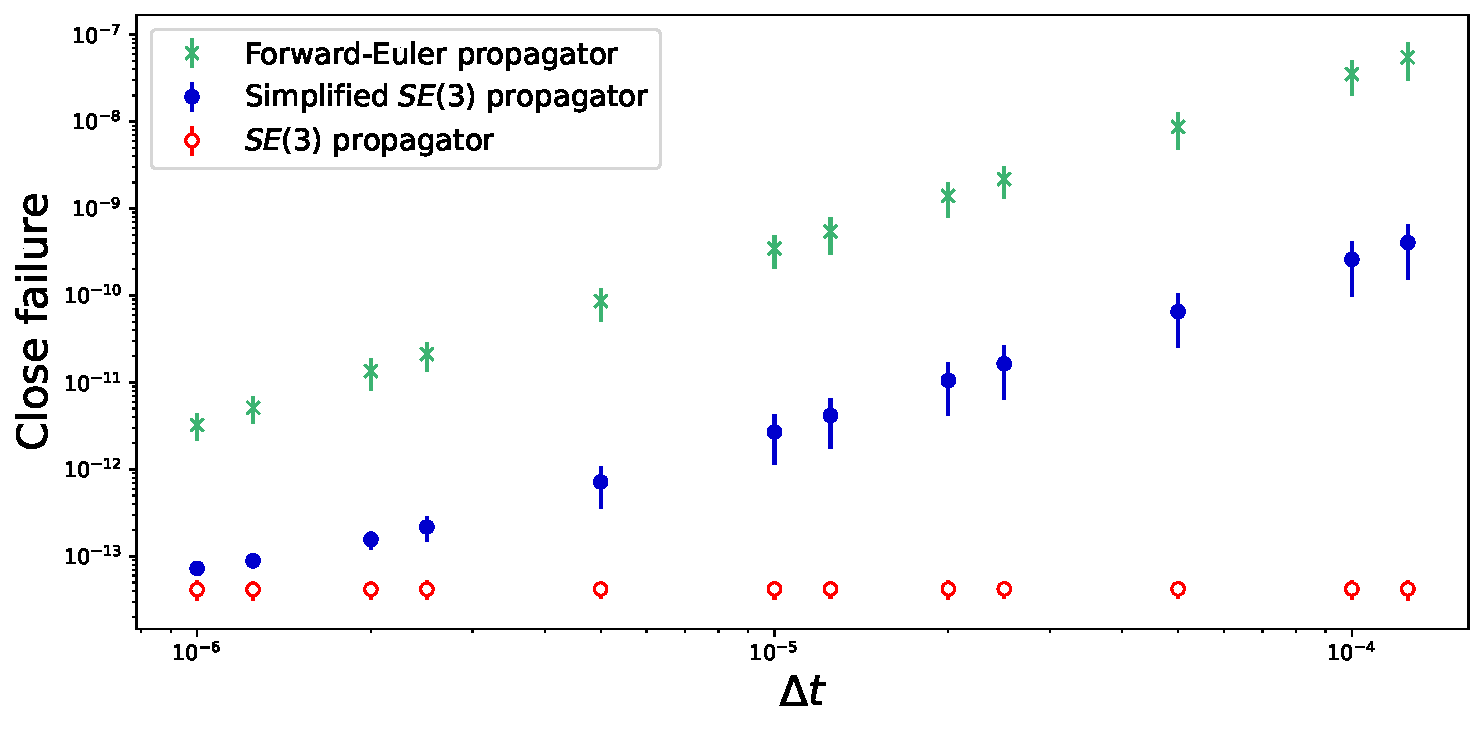
\includegraphics[width=\textwidth]{figs_part2/benchmark_simulations/OD_rod_close_error}
        \caption[]%
        {}    
        \label{fig:OD_rod_close_error}
    \end{subfigure}
    
    \vskip\baselineskip 
    
    \begin{subfigure}[b]{0.76\textwidth}
        \centering
        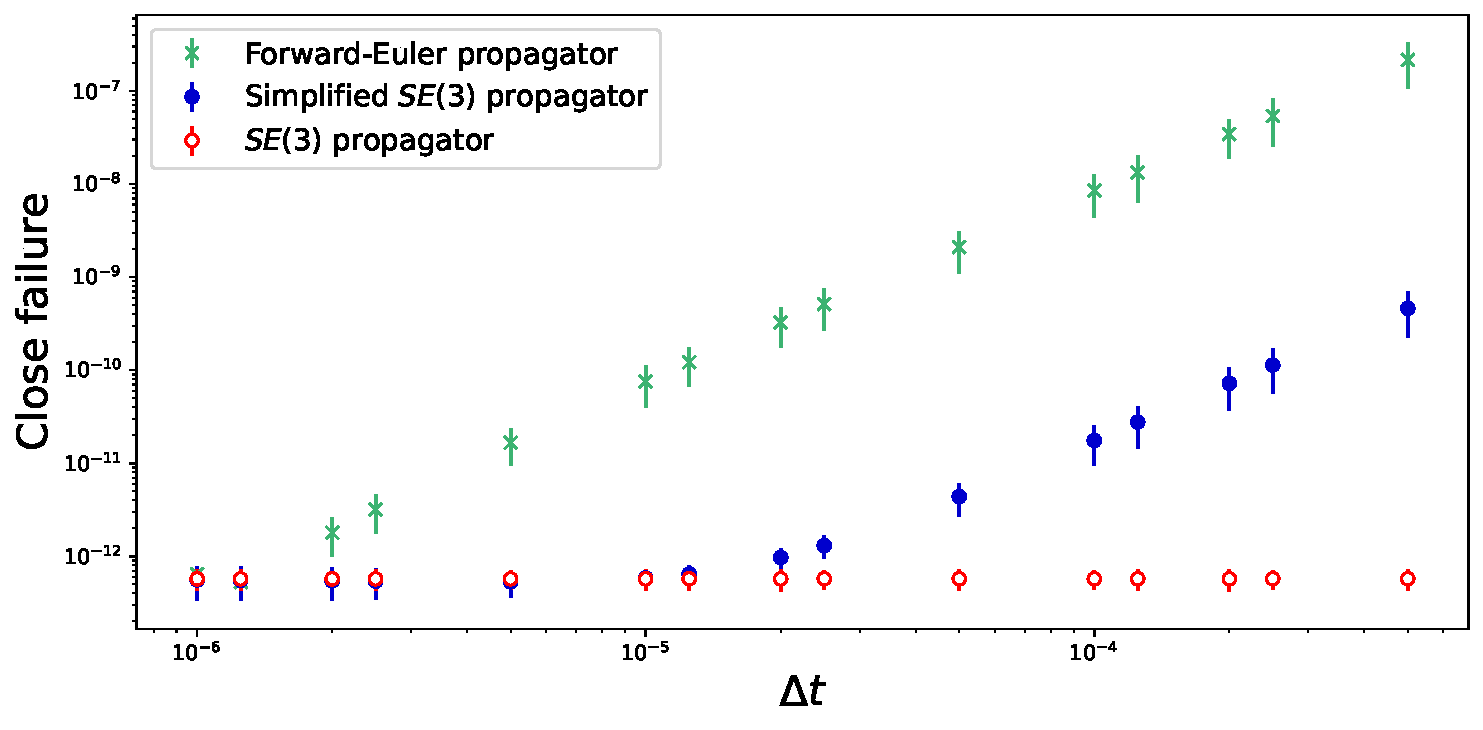
\includegraphics[width=\textwidth]{figs_part2/benchmark_simulations/UD_rod_close_error}
        \caption[]%
        {}    
        \label{fig:UD_rod_close_error}
    \end{subfigure}    
    
    \vskip\baselineskip   
    
    \begin{subfigure}[b]{0.76\textwidth}
        \centering
        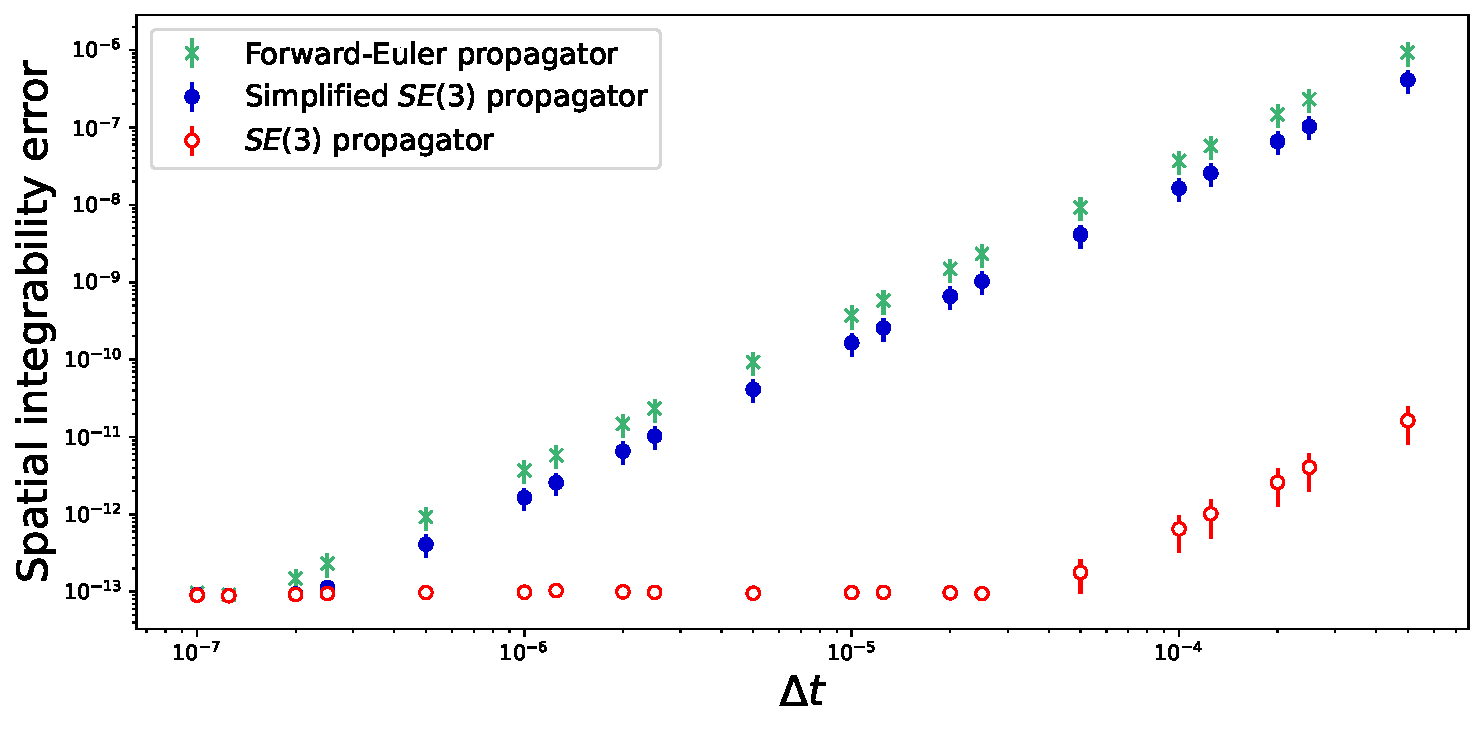
\includegraphics[width=\textwidth]{figs_part2/benchmark_simulations/KE_surface_integrability_error}
        \caption[]%
        {}    
        \label{fig:KE_surface_integrability_error}
    \end{subfigure}

    \caption[  ]
    {\small (a and b) The mean closure failure of a $N_\text{sim} = 50$ benchmark simulations of closed Cosserat rods undergoing overdamped and underdamped dynamics respectively, as a function the time-discretisation $\Delta t$, integrated using the given short-term propagators. We see that the $SE(3)$ propagator preserves the closed loop of the rod up to near-machine precision. (c) The spatial integrability error $\Delta^\text{int}_{uv}$ as a function $\Delta t$ of a Cosserat sheet, as a result of kinematically propagating it using the given short-term propagators. We see that the $SE(3)$ propagator preserves spatial integrability where the simplified $SE(3)$ and the Forward-Euler propagators fail to do so.} 
\end{figure*}

Here we compare the performance of the Forward-Euler Eq.~\ref{eq:FE scheme}, the $SE(3)$ and the simplified $SE(3)$ propagators in numerics. In simulations, we have observed that the latter two propagators enjoy smaller errors in general during numerical integration. However, the main benefit of geometric integrators are that they preserve the geometric structures of the systems. We consider three systems: Overdamped Cosserat rod kinodynamics (see \ref{eq:Cosserat rod overdamped dynamics}), underdamped Cosserat rod kinodynamics (see Eq.~\ref{eq:underdamped cosserat rod}) and Cosserat surface kinematics (see Eq.~\ref{eq:cosserat surface eom}).

For the Cosserat rod systems, we considered a random initial \textit{closed} configuration (see Fig.~\ref{fig:example random initial cosserat configuration} for an example), under the influence of randomly configured constitutive forces and moments. We then simulated the systems until a time $T$, and computed extent to which the rod \textit{fails to be closed} at $T$. In other words, if $\Phi(u,t)$ is the spatio-temporal configuration of the simulated rod, we compute the distance $|\Phi(L_0, T) - \Phi(0, T)|$, which is \textit{closure failure} of the rod. Due to numerical errors, rods that are initially configured as closed will in general fail to remain so. For a range of time-discretisations $\Delta t$, we simulated $N_\text{sim} = 50$ random configurations, and found the resulting closure failures. We then computed sample means and variances of the closure failures as a function of $\Delta t$. The results are shown in Fig.~\ref{fig:OD_rod_close_error} and Fig.~\ref{fig:UD_rod_close_error} for the overdamped and underdamped systems respectively. We see that the simplified $SE(3)$ propagator outperforms the Forward-Euler, however the closure error for the $SE(3)$ propagator is vanishingly small and near machine precision. We also see that the $SE(3)$ propagator is consistent in this regard, with its relatively small sample variances.

For the Cosserat surface, we considered an initial conditional of a flat sheet with a constant perpendicular material frame, that is then subjected to a random velocity and angular velocity profiles. We then computed the short-term propagator for a given time-discretisation $\Delta t$. On the resulting propagated state, we computed the supremum of the residual integrability error $\Delta^\text{int}_{u v}$, given in Eq.~\ref{eq:spatial integrability residual} over the material base space. As for the Cosserat rod, we performed $N_\text{sim} = 50$ random simulations for each $\Delta t$, and computed the sample mean and variance of the error. The results are shown in Fig.~\ref{KE_surface_integrability_error}. Here we see again that the simplified $SE(3)$ propagator has a slightly improved performance relative to the Forward-Euler propagator. The full $SE(3)$ propagator however preserves the spatial integrability of the near machine precision for $\Delta t \leq 5 \times 10^{-5}$.

 We briefly explain the relevance of the residual integrability error: If the $\Delta^\text{int}_{u v} \neq 0$ then the spatial reconstruction fields $X_\alpha$ do not satisfy the spatial integrability conditions Eq.~\ref{eq:(summary) spatial integrability condition}. In practical terms, this means that $X_\alpha$ do not integrate to a a unique spatio-temporal configuration $\Phi$ (the specific $\Phi$ that is computed would be dependent on the path taken in the reconstruction). Furthermore, in Eq.~\ref{eq:(summary) time derivative of spatial integrability conditions} we see that integrability errors suffer exponential growth. Thus, simulations using non-geometric integrators will in general require intermittently stopping to re-spatially integrate $X_\alpha$ in order to maintain the errors. We thus see the importance and utility of constructing a geometric integrator for a given $G$-configured system.

\chapter{Conclusion}


More work can be done on Lie group integrators. Im only using the vanilla version. Can also do operator splitting to consider the derivatives as well (integrating factor).
